%%%%%%%%%%%%%%%%%%%%%%%%%%%%%%%%%%%%%%%%%%%%%%%%%%%%%%%%%%%%%%%%%%%%%%%%%%%%%%%%%%%%%%%%%%%%%%%
%PACKAGES
%%%%%%%%%%%%%%%%%%%%%%%%%%%%%%%%%%%%%%%%%%%%%%%%%%%%%%%%%%%%%%%%%%%%%%%%%%%%%%%%%%%%%%%%%%%%%%%
\documentclass[a4paper, 11pt, abstracton]{extarticle}
%\usepackage[top=3cm,right=2.5cm,bottom=2.5cm,left=2.5cm]{geometry}
\usepackage[top=25.4mm,bottom=25.4mm,left=25.4mm,right=25.4mm]{geometry} % Document margins
\usepackage{setspace}\setstretch{1.5}
\usepackage[ngerman,USenglish]{babel}
\usepackage[utf8]{inputenc}
\usepackage[para,online,flushleft]{threeparttable}
\usepackage{lscape}
%\usepackage{fixltx2e}
\usepackage{amsmath}
\usepackage{placeins}
\usepackage{amsfonts}
\usepackage{amssymb}
\newcommand{\sym}[1]{\rlap{#1}}
\usepackage[hidelinks]{hyperref}
\usepackage{makeidx}
\usepackage{comment}
\usepackage{amsthm}
\usepackage{verbatim}
\newtheorem{proposition}{Proposition}
\newtheorem{result}{Result}
\usepackage{graphicx}
\usepackage{morefloats}
\usepackage{rotfloat}
\usepackage{float}
\usepackage{adjustbox}
\usepackage{multirow}
\usepackage{caption}
\usepackage{subcaption}
\usepackage{lipsum}
\usepackage{eqnarray}
\usepackage{tabulary}
\usepackage{tabularray}  % For talltblr, Q columns, etc.
\UseTblrLibrary{booktabs}
\usepackage{dcolumn}
\usepackage{paralist}
\usepackage{xcolor}
\usepackage{titling}
% If within loop
\usepackage{pgffor}
\usepackage{epsfig}
\usepackage{epstopdf}
\usepackage[space]{grffile}
\usepackage{siunitx}
\usepackage{makecell} %mutlilinetables
\usepackage{enumitem}
\usepackage{ragged2e}
\usepackage[version=3]{mhchem}
\usepackage{fancyhdr}
\pagestyle{fancy}
\fancyhf{}
% this line is added to remove the top line
\renewcommand{\headrulewidth}{0pt}
\cfoot{\thepage}
\newcommand\fignote[1]{\captionsetup{font=footnotesize}\caption*{#1}}
\usepackage{float}
\floatplacement{figure}{ht}
\usepackage{url}
\usepackage{import}
\usepackage{ucs}
\usepackage{natbib}
\usepackage{booktabs}
\usepackage{tabularx}
\usepackage{tikz}
\newcommand{\inputTikZ}[2]{%  
     \scalebox{#1}{\input{#2}}  
	}
\usetikzlibrary{patterns}
\newenvironment{tikzschriftgroesse}{\begin{small}}{\end{small}}
\usepackage{pgfplots}
\pgfplotsset{compat=newest,compat/show suggested version=false}
\usepgfplotslibrary{polar}
\usepgflibrary{shapes.geometric}
\usetikzlibrary{calc}
\usetikzlibrary{decorations}
\usepackage{enumitem} 
\usepackage{framed}
\usepackage[toc,page]{appendix}
%only for huxtables:
\usepackage{hhline}
\usepackage{colortbl}
\usepackage{placeins}
\usepackage{titling}
\newcommand{\logo}[1]{%
  \postauthor{%
  \end{tabular}\par\end{center}
  \begin{center}
  \vskip8.0em
  \inclu
  degraphics[scale=0.22]{#1}
  \end{center}
  \vskip4.0em}%
}
%in order to center the figures:
	\makeatletter
	\g@addto@macro{\figure}{\centering}
	\makeatother
%in order to center the tables:
	\makeatletter
	\g@addto@macro{\table}{\centering}
	\makeatother

\maxdeadcycles=1000

\makeatletter\let\expandableinput\@@input\makeatother


%Fonts (XeLaTeX with fontspec for native Unicode support — fixes € and ’ rendering)
\usepackage{fontspec}
\setmainfont[SmallCapsFont={Latin Modern Roman Caps}]{Latin Modern Roman}
\setsansfont{Latin Modern Sans}  % was: \usepackage{avant}; Latin Modern Sans is the natural companion to LM Roman/Mono and ships with TinyTeX
\setmonofont{Latin Modern Mono}
\setlength{\parindent}{1cm}

% Set path for graphics


%***************************************************************************************
\usepackage[labelfont=bf]{caption} %make Table~labels bold

	\usepackage{fancyhdr} % Headers and footers
	\pagestyle{fancy} % All pages have headers and footers
	%\fancyhead{} % Blank out the default header
	\fancyfoot{} % Blank out the default footer
	%\fancyhead[C]{\footnotesize{Immigrating into a Recession}} % Custom header text
	%\fancyfoot[RO,LE]{\thepage} % Custom footer text
	\fancyfoot[C]{\thepage} % Custom footer text center's page number
	%\pagenumbering{Roman} %If I want Roman Numeral page numbering

\usepackage{longtable}


\title{\centering Opportunities or Benefits: Local Conditions and Refugee Labor Market Integration}

\author{Katia Gallegos Torres, Andreas Steinmayr, Valentin Wett\thanks{We would like to thank  Olof Åslund, Cevat Aksoy, Frederic Docquier, Martin Fernandez, Tina Hinz, Michael Siegenthaler, Jan Stuhler, and participants of various seminars and workshops for helpful comments and suggestions. Andrea Buchacher and Karolina Hanger provided valuable research assistance. We acknowledge the financial support by the Faculty of Economics and Statistics at the University of Innsbruck. Gallegos Torres acknowledges financial support from the German Federal Ministry of Labor and Social Affairs through the Fördernetzwerk Interdisziplinäre Sozialpolitikforschung (FIS) under grant number FIS.00.00140.19. The computational results presented here have been achieved using the LEO HPC infrastructure at the University of Innsbruck. All remaining errors are our own.
\newline Contact: Katia Gallegos Torres, IAB Nuremberg and ZEW Mannheim, \href{mailto:Katia.Gallegos-Torres@iab.de}{Katia.Gallegos-Torres@iab.de}; Andreas Steinmayr, University of Innsbruck, CESifo, Rockwool Foundation, IPL and IZA, \href{mailto:andreas.steinmayr@uibk.ac.at}{andreas.steinmayr@uibk.ac.at}; Valentin Wett}}

\date{This version: \today.}

\begin{document}

%%%%%%%%%%%%%%%%%%%%%%%%%%%%%%%%%%%%%%%%%%%%%%%%%%%%%%%%%%%%%%%%%%%%%%%%%%%%%%%%%%%%%%%%%%%%%%%
%TITLE PAGE	
%%%%%%%%%%%%%%%%%%%%%%%%%%%%%%%%%%%%%%%%%%%%%%%%%%%%%%%%%%%%%%%%%%%%%%%%%%%%%%%%%%%%%%%%%%%%%%%

\maketitle

\thispagestyle{empty} 
  
\begin{abstract} 
This paper studies how local labor market tightness and welfare benefit levels at the time of receiving protection shape refugees’ labor market integration and location choices. Exploiting a sequence of reforms that generated quasi-random variation in benefit levels and labor market tightness across initial placements, we find that tighter local labor markets raise employment, while more generous benefits slightly reduce it. These effects persist for about 2.5 years, but both shocks have lasting impacts on internal migration. Moreover, the negative employment effect of benefits is larger in tighter labor markets. Neither shock changes the probability of leaving Austria altogether.

\end{abstract}

\vspace{1em}

JEL codes: F22, J31, J61 

Keywords: Immigrant integration, refugees, welfare benefits, labor demand

\newpage
\setcounter{page}{1}


%%%%%%%%%%%%%%%%%%%%%%%%%%%%%%%%%%%%%%%%%%%%%%%%%%%%%%%%%%%%%%%%%%%%%%%%%%%%%%%%%%%%%%%%%%%%%%%
% MAIN PART
%%%%%%%%%%%%%%%%%%%%%%%%%%%%%%%%%%%%%%%%%%%%%%%%%%%%%%%%%%%%%%%%%%%%%%%%%%%%%%%%%%%%%%%%%%%%%%%


\section{Introduction}
%%%%% Note from KGT: KEEP IN MIND WHAT AN INTRO SHOULD CONTAIN! %%%%%%%
% source: https://dominika-langenmayr.net/wp-content/uploads/2022/09/Session-5_VL.pdf
% 1. Motivation (1 paragraph) , i.e. the hook
% 2. Research question  (1 paragraph) --> place it in the literatzre
% 3. Main contribution (2-3 paragraphs) , lead with our findings then how it extends the literature
% 4. Methods (1-2 pagraphs)
% 5. Findings (2-3 paragraphs) (optional, mention robustness)
% 6. Roadmap

The economic and social integration of refugees remains a central policy challenge across advanced economies \citep{brell_labor_2020}. Governments implement a range of policies not only to foster integration but also to shape migration flows, manage fiscal resources, and sustain public support for hosting refugees.\footnote{We use the term refugee for an individual whose asylum application was approved \citep{hatton2020}. We use the term asylum-seeker specifically for a person before being granted protection.} Some policies restrict refugees’ choices—such as dispersal rules that allocate them across regions—while others provide incentives, for instance by changing benefit generosity to foster labor market participation. Yet integration outcomes also depend on factors beyond policymakers’ control, including the absorptive capacity of local labor markets. Ultimately, successful integration hinges on how refugees respond to these policy environments and labor market conditions. Understanding these responses, and the ways in which different policies interact, is therefore critical for designing effective refugee integration strategies \citep{adda2022}.

We study how refugees adjust their labor supply and relocation decisions once restrictions on mobility and employment are lifted. Specifically, we examine how local labor market tightness and welfare benefit levels—individually and in interaction—shape refugees’ choices. Austria provides a particularly well-suited setting for this analysis. During the asylum process, refugees are subject to a dispersal policy and face strict limits on employment and relocation. These restrictions are lifted immediately upon recognition, at which point refugees gain full access to the labor market and freedom of movement across states. Three features make Austria distinctive. First, the sharp shift from restricted to unrestricted choice allows us to combine quasi-experimental variation in initial placement with observation of behavior under full mobility. Second, because most refugees must vacate their assigned accommodation within four months, they are forced to make consequential labor market and residential decisions in a compressed time frame, resembling the incentives embedded in work-first policies \citep{arendt_labor_2022, arendt_trade-offs_2023}. Third, Austria’s federal welfare system generates large and time-varying cross-state differences in benefit generosity, enabling us to test whether refugees respond to financial incentives by relocating to more generous states.\footnote{For example, in 2015, a single refugee with subsidiary protection in Carinthia received only €200 in basic subsistence support, compared to more than three times that amount in Tyrol or Vienna.}

We find that many refugees relocate immediately once restrictions are lifted: roughly 30 percent of those initially placed outside Vienna move to the capital within four months, despite Vienna having a relatively weak labor market. Both local labor market tightness and welfare generosity at the assigned location shape this decision. Tighter labor markets—especially in low-barrier occupations—induce higher and more immediate labor force participation among men, which in turn increases the probability of remaining in the assigned state. While these employment effects are temporary, location choices are persistently affected.

Benefit generosity also influences outcomes, though more modestly. A decrease in monthly benefits increases the propensity to relocate and male employment temporarily and female employment more persistently. Importantly, these effects interact with labor market conditions: benefit reductions significantly increase employment only when local labor markets are tight, consistent with recent evidence from Denmark \citep{dustmann2024}. Taken together, our results suggest that mobility responses primarily reflect adaptation to immediate constraints rather than forward-looking optimization over longer-term labor market prospects. Consequently, the combination of dispersal policies with subsequent unrestricted mobility does not contribute to "greasing the wheels" of the labor market \citep{borjas2001}.

Our contribution is threefold. First, we provide causal evidence on how local labor market conditions at the time of labor market entry shape refugees’ employment and mobility decisions. Second, we examine how cross-state differences in welfare benefit generosity influence both relocation and labor supply, thereby speaking to the welfare magnet hypothesis. Third, we analyze how local conditions and the policies in place interact, showing that the effects of welfare policies on employment are amplified when local labor markets are tight. Together, these findings inform academic debates on immigrant location choice and labor market assimilation, while also providing timely evidence for policymakers designing refugee integration policies.

We now turn to a more detailed description of our setting, data, methodology and results. We draw on the Austrian asylum system, which combines quasi-random assignment of asylum-seekers across regions with sharp changes in mobility and labor market access once protection is granted. This institutional structure creates exogenous variation in the local conditions refugees face at the time of labor market entry. Welfare benefits, set at the federal-state level, varied substantially across states, over time, and by protection status. Between 2015 and 2017, several states implemented large benefit cuts, some of which were later overturned by courts, further increasing variation in generosity. 

Our analysis uses administrative data covering more than 40,000 refugees who arrived between 2011 and 2018, providing complete information on employment trajectories, social security contributions, and place of residence. Unlike related studies \citep{ferwerda2023, dustmann2024, azlor_local_2020}, we can exploit both spatial and temporal variation in local labor market tightness and welfare benefit levels, which allows us to separate their effects and better account for regional confounders.

The data also contain detailed records on job openings, which enable us to measure both the overall tightness of the local labor market and the demand for specific occupations. These features of the Austrian setting allow us to examine how refugees respond to both labor market opportunities and financial incentives at the time their choice set expands.

An interquartile increase in local labor market tightness—about 0.2 additional vacancies per unemployed person—raises the probability of employment twelve months after recognition by 4.2 percentage points and reduces welfare use. The effect fades after roughly 30 months. Labor market tightness also increases the probability of remaining in the assigned state and decreases relocation to Vienna, the primary destination for movers. By contrast, lower benefit levels have modest effects: a reduction of €100 increases employment after one year by 0.5 percentage points and monthly earnings by about €10, while decreasing the probability of remaining in the assigned state by one percentage point. These employment effects dissipate after 2.5 years, but location effects persist. Neither labor market tightness nor benefits affect the probability of leaving Austria altogether. Finally, consistent with \citet{dustmann2024}, benefit reductions both raise employment and reduce welfare take-up only when local labor markets are tight.

%Austria received asylum applications at a rate above the EU average.\footnote{During 2014--2018, the EU average was two first applications per 1,000 inhabitants. Austria received four applications per 1,000 \citep{eurostat_2023}.} 
%We use administrative data, which contains the full labor market trajectories, social security insurance spells and place of residence for over 40,000 refugees arriving in Austria from 2011 to 2018. Identification is based on the initial exogenous distribution and the restrictions during the asylum process. Variation in labor demand and benefit levels over time and space allows us to identify their effects separately but also study how they interact. Unlike related studies \citep{ferwerda2023, dustmann2024, azlor_local_2020}, we can use spatial and temporal variation in labor demand \emph{and} benefit levels, which allows us to better control for potential regional confounders.

%The data includes comprehensive and detailed information on job openings, which helps us assess labor demand by quantity and type of jobs in their assigned regions. Additionally, refugees encounter heterogeneous welfare benefits set by federal states, which underwent several reductions between 2015 and 2017, though the courts later overturned some of these cuts. Consequently, benefit levels differ markedly across states, over time, and according to the type of protection granted. 

%Our main findings are as follows. An interquartile increase in local labor demand, equal to 0.2 additional open positions per unemployed person, increases the employment probability 12 months after protection by about 4.2 pp and consequently reduces welfare use. The effect dissipates after 30 months. Effects on earnings are driven by higher employment and not by higher wages. %, similar to the one found in \citet{barsbai2024} for family migrants in the US.
%Higher labor demand increases the probability of remaining in the state of assignment and reduces the probability of moving to Vienna, the preferred destination of refugees who move within Austria. The effect of higher benefits is mirrored but small: 100 euro higher benefit levels reduce the employment probability 12 months after protection by 0.5 pp. and monthly earnings by about 10 euro. Consequently, changes in benefit levels result in large changes in disposable income. However, the effects on employment dissipate after about 2.5 years. At the same time, 100 euro higher benefit levels persistently increase the probability of remaining in the state by about one pp. Neither local labor demand nor benefit levels affect the propensity to leave Austria entirely.

%Similar to \cite{dustmann2024}, we find that the effects of labor demand and benefit levels interact in significant ways. The effect of a reduction in benefit levels on employment after one year is large when labor demand is high and negligible otherwise. Conversely, lowering benefits when labor demand is high reduces the take-up of benefits but has no effect if labor demand is low.

%Our fine-grained data allows us to study the timing of events in detail. The effect of high labor demand materializes within three months. 

We contribute to several strands of literature that are usually studied in isolation but are nonetheless closely interlinked.

% Location choice of immigrants - in general and with respect to labor market and welfare generosity

\textbf{Location choice of immigrants.} The question of how immigrants choose a location has received extensive attention in the literature, but several issues remain contentious, such as the extent to which differences in welfare benefits and labor demand influence this decision. An empirical regularity observed in many contexts is that immigrants tend to cluster in large cities \citep{monras2023}. Our context is no exception, with widespread relocation to Vienna as soon as this becomes possible. This phenomenon has been explained by higher place utility offered by cities, for example, through the existence of ethnic enclaves or amenities such as educational institutions \citep{damm2010}. Another potential explanation is that migrants choose high-cost–high-income cities, as they consume a smaller share of their income locally and thus benefit disproportionately from higher wages \citep{albert2022}. The labor market is unlikely to play an important role as a pull factor in our context. Vienna is one of the locations with the lowest labor demand, especially for low-skilled jobs; average wages for blue-collar workers are below the Austrian average (€30,509 vs. €35,564);\footnote{\url{https://www.statistik.at/fileadmin/publications/Allgemeiner_Einkommensbericht_2020.pdf}} and refugees in Vienna have some of the lowest employment rates in the country. As the labor market does not seem to draw refugees to Vienna, other explanations—such as networks, amenities, and benefit generosity—are likely to play a more important role.

Given the strong concentration of refugees in a single destination and the absence of significant benefit changes in Vienna, we do not seek to identify which factors attract them to particular locations (pull) but rather which characteristics of their assigned locations push them away. Such push models have been used to study immigrants’ location preferences, but for causal identification they require exogenous placement into initial locations \citep{damm2009}, which is the case in our setting.

\citet{borjas2001} argues that migrants, who are less attached to a particular location and thus face lower moving costs, contribute to \textit{greasing the wheels} of the economy by avoiding areas where their skills are not in demand. Migrants reacting to local conditions through outmigration or staying is part of this process. Our results suggest that refugees do respond to the availability of jobs in their initial regions. However, they do not seem to select the subsequent regions based on labor market prospects. %However, these responses appear to ease short-term constraints rather than reflect longer-term optimization of earnings potential.

We also contribute to the question of whether the generosity of welfare benefits affects immigrants’ location choices—known as the \textit{welfare magnet hypothesis} \citep{borjas1999}. This question has received considerable attention. \citet{agersnap_welfare_2020} study the same Danish reform analyzed in \citet{dustmann2024} and show that the benefit reduction lowered migrant inflows with an implied elasticity of 1.3.\footnote{\citet{adema2025} discusses several methodological concerns with this study and argues that the elasticity is about 0.28 for new arrivals.} At the subnational level, \citet{ferwerda2023} study Switzerland and examine how the generosity of benefits in refugees’ initial placement locations affects subsequent relocation. This push approach is very similar to ours. They find that higher benefits reduce relocation, but only to a minor extent—at most two pp., even for very large differences in benefits. Our estimates of roughly one pp. for a €100 change in benefits are considerably larger. Exploiting some of the same reforms that we analyze, \citet{huber_impact_2022} find in an event-study design that reductions in benefit levels trigger significant outmigration. 



%The question of how immigrants choose a location has received extensive attention in the literature but several questions remain contentious, such as to what extent differences in welfare benefits and labor demand influence this decision. An empirical regularity observed in many contexts is that immigrants tend to cluster in large cities \citep{monras2023}. Our context is no exception with the widespread relocation to Vienna as soon as this is possible. This phenomenon has been explained with higher place utility offered by cities, e.g., through the existence of ethnic enclaves but also amenities such as educational institutions \citep{damm2010}. Another potential explanation is that migrants choose high-cost-high-income cities as they consume a smaller share of their income in this location and thus benefit disproportionately from the higher wages \citep{albert2022}. The labor market is unlikely to play an important role as a pull factor in our context. Vienna is one of the locations with the lowest labor demand, especially for low-skilled jobs; average wages for blue-collar workers are below the Austrian average (30,509 vs. 35,564 euro)\footnote{\url{https://www.statistik.at/fileadmin/publications/Allgemeiner_Einkommensbericht_2020.pdf}}; and refugees in Vienna have some of the lowest employment rates in the country.

% (see Section XX) ADD DESCRIPTIVES HERE
% CITE OECD REPORT HERE

%Given the strong concentration of refugees in one destination within Austria, we do not seek to identify which factors attract them to a certain destination (pull) but rather which factors of their assigned location push them away. Such push models have been used to learn about immigrants' location preferences, but for causal identification, they require exogenous placement into initial locations \citep{damm2009}, which is the case in our setup.

%\cite{borjas2001} argues that migrants, who are less attached to a particular location and thus have lower moving costs, contribute to \textit{greasing the wheels} of the economy by not moving to areas where their skills are not in demand. Migrants reacting to local conditions with outmigration/staying is part of greasing the wheels. Our results suggest that migrants do react to the availability of jobs in their initial region. However, these appear to relax their short-term constraints  and are not the result of longer-term optimization of their earnings potential.

%We also contribute to the question of whether the generosity of welfare benefits affects immigrants' location choices---known as the \textit{welfare magnet hypothesis} \citep{borjas1999}. This question has received considerable attention. \cite{agersnap_welfare_2020} study the same Danish reform as studied in \cite{dustmann2024} and show that the benefit reduction reduced migrant inflows with an implied elasticity of 1.3. At the sub-national level, \cite{ferwerda2023} study for Switzerland, how the generosity of benefits in the place where refugees were initially placed affects their subsequent relocation. This push approach is very similar to ours. They find that higher benefits decrease the incidence of relocation, but only to a minor extent. At most, by two pp., even for very large differences in benefits. Our estimates of a roughly one pp. change for a 100 euro change in benefits is considerably larger. Exploiting some of the same reforms that we look at, \cite{huber_impact_2022} find in an event study approach that reductions in benefit levels trigger significant outmigration.

% ANDREAS: I DROPPED THIS SECTION FOR NOW TO SHORTEN THE INTRO
%\textbf{Dispersal policies.} Many countries have introduced dispersal policies that distribute refugees according to some administrative rules. Through dispersal policies, countries seek to overcome the strong concentration of refugees in certain locations, use resources such as housing more evenly, and increase the acceptance of hosting refugees in the native population. Evidence on the effects of dispersal policies on refugee integration is scarce but the available evidence suggests that refugees subject to a dispersal policy are less integrated into the labor market than refugees who could choose their location themselves \citep{edin2004, fasani_struggle_2022}. While we cannot directly identify the effect of a dispersal policy, the Austrian context is interesting as it combines exogenous assignment through a dispersal policy during the asylum process with no relocation restrictions after getting protection.\footnote{This differs, for example, from the Swiss \citep{bansak_improving_2018} or Danish dispersal \citep{azlor2020} policies where refugees are prohibited or at least severely restricted to remain in the original location for multiple years after being granted protection.} Thus, the policy helps us to overcome the often observed self-selection of immigrants with favourable characteristics into locations with favourable labour market conditions \citep{azlor2020}. But at the same time, we can still observe the refugees' choices after they received protection. 

% Effects of dispersal policies

% many countries have dispersal policies. whats special about austria is that there is a dispersal policy but after status is granted, migrants are free to settle in the entire country. even more, KONs need to find new housing 4 months after status is granted.
% the idea of dispersal policies is to use resources more evenly but also to increase acceptance of hosting refugees in the native population.
%Valentin: in optimum, forward looking migrants should select a location based on their expected integration chances. however, it's more likely that the base their decisions on immediate opportunities and constraints.
% Several countries have started considering dispersal policies that place refugees already in the beginning according to individual integration chances.
% Municipalities could consider asking for refugees that fit their labor demand. however, a given refugee needs a lot of time before he/she gets access to the labor market.
%Migrants incur costs if they are at a suboptimal location initially and need to move. Local knowledge is lost
%We see huge effects for "preferred occupations"

%refugees have to make very consequential decisions within a short period of time.

%In a study for Sweden, Edin et al. (2004) show that, relative to refugees who arrived before the introduction of the policy (and were therefore free to choose where to settle), dispersed refugees were less likely to be employed, had lower earnings and claimed more welfare benefits. These findings are confirmed by Åslund and Rooth (2007). In the context of the Danish dispersal policy, instead, Damm and Rosholm (2010) provide evidence that relocation from the originally assigned location had a large positive effect on the probability of finding employment. 
% Our study is related to three existing impact evaluations that exploit spatial dispersal policies on refugees in Scandinavia to identify the causal effect of local labour market conditions on immigrant labour market outcomes: Åslund and Rooth (2007) for Sweden, Damm and Rosholm (2010) for Denmark and Godøy (2017) for Norway. While our study provides quasi-experimental estimates of the effects of the initial employment rate in the assigned location as well as for a range of alternative measures of local labour market conditions on immigrant employment, Åslund and Rooth (2007) estimates the effects of the initial local unemployment rate on both immigrant earnings and employment. Godøy (2017) , instead, estimates the effects of the initial regional employment rate of non-OECD immigrants on immigrant earn- ings, whereas Damm and Rosholm (2010) exploits the first Danish Spa- tial Dispersal Policy on refugees in place from 1986–1998 to provide quasi-experimental evidence on local determinants on the hazard rate into first job. (Azlor et al. 2020)
% 
%Higher non-western immigrant share decreases the likelihood of moving out. higher co-national share has the same effect but not precisely estimated. Commuting opportunities have no effect.

% refer to our model as a push model (see Hangartner et al 2023). An alternative way of learning about immigrants’ location preferences is to estimate push factors, i.e. the set of negative or positive social or economic factors in an area of origin which pushes migrants away (Lee 1966), based on immigrants’ subsequent internal migration pattern. However, push factor estimates may be biased if immigrants sort into initial locations based on unobserved personal attributes that also influence the secondary migration probability. (Piil Damm 2009)

%Four theories of migrant location choice: welfare magnet (Borjas), greasing the wheels (Borjas), high-income-high-cost (Monras), ethnic enclaves
%Thomas Bauer also has several papers on migrants' location choice.
%Vienna has the lowest labor demand and relatedly low wages, especially for blue-collar workers. In 2017, a blue-collar worker in Vienna had a gross income of 30.509 Euro, while the Austrian average was 35.564 Euro. 
%Vienna has lots of social housing but to qualify, refugees need to have lived in Vienna for more than two years -> no immediate solution.
%Introduce concept of place utility (Piil Damm and Rosholm (2010)). Location choice depends on place utility and earnings (income + benefits).


% highlight Dustman et al (2023), Hangartner et al (2023), and Fasani & Minale? as closest papers
% our mobility effect is somewhat larger than from hangartners push model. they find that mobility decreases by at most 2pp. when going from a very low to very high benefits.
% what makes our empirics better than hangartner, dustmann but also early papers on initial conditions is that we have both, variation in benefits and economic conditions over time. they only have it one dimension, requiring stronger assumptions for identification
% refugee migration is an urban phenomenon. Monras argues that migrants go to expensive cities as the consume a smaller part of their income locally. however, since the labor market in Vienna is so difficult for migrants, the argument does not really work in this context.



%Conditions are very similar to Denmark with refugees not allowed to work. But "The new legislation further strengthened the effort to allocate refugees across all municipalities in the country and made eligibility to means-tested welfare benefits during the 3-year introduction programme conditional on residing in the assigned municipality." 
% The most extensively studied context concerning the effects of dispersal policies and refugee integration more generally is Denmark (CITE XXX). However, the Danish and Austrian context differ in a key dimension. In Austria, asylum-seekers are placed in a particular municipality and are free to settle in the entire country upon receiving protection status. In Denmark, asylum-seekers are hosted in remote reception centers during the asylum process and are only placed in a municipality once they receive protection status. They are then required to remain in the municipality for at least three years, otherwise they loose their protection status. Asylum-seekers can express preferences over locations but these can only be considered when municipality quotas are not yet binding (Azlor et al. 2020).
%Note that the first Danish resettlement policy was different and more similar to the Austrian context without linking residence in the assigned municipality and receipt of benefit. But refugees were assisted in finding housing. Piil Damm and Rosholm (2010) exploit this dispersal policy.

% Effects of initial conditions

\textbf{Effect of initial labor market conditions.} Our findings on the effect of labor market conditions when entering the labor force complement active literature on initial conditions' (long-term) effects for refugees \citep{aslund_when_2007, godoy_local_2017, fasani_struggle_2022, aksoy_first_2023} and immigrants more generally \citep{chiswick1997, chiswick2002, barsbai2024}.\footnote{\citet{von_wachter_persistent_2020} provides a summary of the findings of graduating during different points of the business cycle on life outcomes: On average, entering the labor market in a recession reduces earnings, and these effects persist for up to 15 years, with large heterogeneities by socio-demographics (e.g., education, race, sex). For Austria, \citet{brunner_impact_2014} find that for labor market entrants during 1978-2000, a one pp. higher initial local unemployment rate decreases wages by about 1.3\% over the life cycle and persists for 20 years after labor market entry.} Our detailed administrative data on vacancies and unemployment allows for several refinements compared to previous work. First, we consider the conditions in the district and time of receiving unrestricted labor market access instead of at arrival and thus better capture the relevant moment.\footnote{\citet{aslund_when_2007} discuss which is the relevant initial labor market area since refugees do not immediately enter the labor market.} Second, we use the initial vacancy-to-unemployment ratio ($IVUR$) instead of employment or unemployment ratios because it might be a better measure of local labor market conditions \citep{dustmann2024}. In particular, the measure provides us not only with information on the general state of the labor market but we can identify labor demand for particular skills or individual sectors. Third, variation over time and space allows us to not only rely on cross-sectional variation but also to control for other unobserved regional characteristics that could be correlated with $IVUR$ and confound our results. Fourth, we can also look at the effects on a monthly level, finely capturing any dynamics playing out immediately after getting access to the labor market. Two concurrent papers \citep{degenhardt2025initial, degenhardt2025} exploit the same Austrian dispersal setting to study single labor-market segments (hospitality and gig work, respectively); we compare their findings with ours in Section \ref{sec:mech} alongside our own sectoral decompositions.
Relative to the majority of findings in this literature, we find that the effects of initial labor market conditions on employment are not persistent beyond 2.5 years. This is likely due to a situation where labor supply decisions and location choice are made simultaneously. Conditions right after receiving protection are important to find employment and subsequently housing.\footnote{The only other study we are aware of to analyze the effects on mobility is \citet{barsbai2024}, which finds that family migrants in the U.S. do not move in response to adverse economic conditions. However, unlike refugees, family migrants have strong personal links to the location of initial residence, making any moves more costly.}
%Refugees who face strong labor demand 
Several factors might explain our short-lived effects. First, the good labor market conditions at arrival could push refugees into employment too fast and `hinder' investments in host-country-specific human capital, which would, otherwise, payout in the future \citep{battisti_dynamic_2022}. Second, refugees in Austria are particularly mobile, and the importance of initial local conditions fades away. We also study how initial labor market tightness affects mobility and find persistent effects on the probability of staying in the assigned location. 


%Next, more specifically, we contribute to the literature studying the role of initial local (economic) conditions on refugees` integration outcomes. These initial conditions cover a variety of items and can be grouped as follows \citep{muller_labor_2023}: labor market conditions (e.g., unemployment rates \citep{aslund_when_2007, godoy_local_2017, aksoy_first_2023, muller_labor_2023}, recessions \citep{barsbai2024}), co-ethnic networks \citep{beaman_social_2012, edin_ethnic_2003, battisti_dynamic_2022}, and asylum policies (e.g., employment bans \citep{fasani_lift_2021}, dispersal policies \citep{fasani_struggle_2022}), and local (negative) attitudes \citep{aksoy_first_2023, jaschke_scared_2022, muller_labor_2023}.
%From these papers, those studying the role of unemployment rates have usually overcome selection problems by relying on quasi-random variation provided by, e.g., dispersal policies \citep{aslund_when_2007, godoy_local_2017, aksoy_first_2023, muller_labor_2023} or family reunification policies \citep{barsbai2024}.
%For Sweden, \citet{aslund_when_2007} study the long-term effects of initial local unemployment rates on refugees arriving between 1987 and 1991. For identification, they rely on a refugee settlement policy and find that initial higher local unemployment rates have a long-lasting negative impact on employment and earnings. These appear to be a combination of scarring and lock-in effects. The authors do not only use the initial local unemployment rate but also the one in the second full year after arrival since refugees do not immediately enter the labor market, where the latter is larger than the former.
%\citet{godoy_local_2017} study the role of local conditions---measured by the employment rate of the immigrant population in the initial labor market region---at the time of arrival on labor earnings of refugee immigrants in Norway. She relies on the quasi-random allocation of refugees to identify the effect of the initial immigrant unemployment rate. Interestingly, she finds that the effects are not driven by individual scarring effects but rather by persistent local poor economic conditions together with immobility.
%\citet{muller_labor_2023} study the role of initial conditions (unemployment rate, co-ethnic network, restrictive attitudes) on the integration of refugees in Switzerland during 1998-2018. They study the interplay of local contexts and policies. The authors find significant negative effects of initial unemployment rates and positive effects of initial more restrictive attitudes toward refugees and immigrants on the employment probabilities of refugees. These effects persist for over 16 years after arrival in Switzerland.
%\citet{aksoy_first_2023} study the role of unemployment rates (fixed in 2014) and attitudes towards immigrants on the labor market and social integration of refugees who arrived in Germany during 2013-2018. Using the German socio-economic panel they find that both the unemployment rate and negative attitudes decrease the employment probability of refugees. For identification, the authors rely on the quasi-random allocation of refugees across counties. %, which they validate by showing no correlation between individual-level characteristics and the county-level unemployment rate and attitudes toward immigration.
%Our paper contributes to this literature in several ways. First, we rely not only on the dispersal policy in place but acknowledge that municipalities might prefer to host certain groups. Hence, conditional on arrival-group fixed-effects% (family status*gender*quarter of arrival)


% Effect of welfare generosity


\textbf{Effect of welfare generosity.} Moreover, our work also contributes to a small literature studying the link of welfare generosity and labor market conditions on the integration and welfare use by immigrants \citep{Bratsberg2020ImmigrantGenerosity}. In the most closely related paper, \citet{dustmann2024} study the role of refugee benefit cuts in Denmark in an RD setting. The initial positive employment effects disappeared after 4-5 years. The results further show that the effect is larger in regions with more favorable labor demand conditions. Similar to this study, we also identify the interaction of the effect of these two factors. Our findings corroborate the conclusion of \citet{dustmann2024} as we also see that changes in benefit levels have larger effects on employment rates and welfare use when labor markets are tight.

More broadly, our paper expands on previous literature by looking at the interaction of local conditions and the policies in place. Although several studies have recognized the need for this approach \citep[e.g.,][]{fasani_struggle_2022, muller_labor_2023}, few have incorporated both elements in their analysis. Recent work has examined the combined role of initial labor market conditions and hostile attitudes toward immigrants \citep{muller_labor_2023, aksoy_first_2023, schilling_impact_2021}, but aside from \citet{dustmann2024}, none have focused on the interaction with welfare policies.






%XXXXXXXXXXX




%Since 2015, Europe and, more recently also, the U.S. have seen a sharp increase in asylum applications (UNHCR, 2022). Labor market integration of refugees is of particular importance, with employment rates of refugees often significantly lower than those of natives and other migrant groups \citep{brell2020}. This may result in extended periods of reliance on welfare benefits. Recently, many countries have restricted access to or reduced welfare benefits for refugees. This strategy aims to incentivize greater labor force participation but also to make these destinations less appealing. However, labor demand also plays a crucial role, potentially affecting both labor market integration and the attractiveness of a destination.



% SOME NOTES (ANDREAS)



%Still, the big question is why the "headstart" migrants get in some locations is not converted into a longer-term advantage.
%Danish policy seeks to integrate refugees into low-skilled jobs (Foged and Peri). This might be counterproductive in the longer term.
%Our high-frequency data allows us to study the immediate reaction. The effect of high labor demand occurs almost immediately - after 3 months, the coefficient is already around 0.15. Which is huge relative to the very low baseline. Also the reaction to benefit levels is quick and happens within three months. As a consequence, they stay - we see the immediate location choice influenced.
%even though we see that employment rates are not permanently shifted, location choice is. why? in this initial period migrants need to find an apartment. when they find a job quickly, they also solve the housing question. and then, even if the employment is not permanent, they have settled.
%add scatterplot between IVUR and staying rates


%FURTHER LITERATURE
%For investigations into the effect of ethnic concentration on immigrant labour market outcomes, see Borjas (1995), Beaman (2012), Cutler et al. (2008), Dagnelie et al. (2017), Damm (2009) and Edin et al. (2004), among others.  (from the Minale/Fasani paper)

%Effect of employment rate at arrival is constant for four years.
%The findings of a significant, negative effect of the presence of immigrants and the local population size on the hazard rate into first job both support the assumption underlying dispersal policies, that spatial dispersal of refugees away from immigrant-dense cities promotes economic assimilation of refugees. If the aim of a spatial dispersal policy is to pursue the assimilation motive—the policy should primarily be designed so as to reduce relocation rates while at the same time placing refugees in municipalities where the job finding rate is fairly high. Medium-sized municipalities with access to institutions for vocational and higher education, an appropriate number of co-nationals (but no immigrants of other ethnicities), a large public housing market and a low unemployment rate appear to be well suited for this purpose. (Piil Damm and Rosholm (2009)
%To summarize, refugees prefer living in large cities in part because it facilitates access to housing and educational institutions. (Piil Damm 2009)



%Although we cannot directly test for the quality of the first job, the effect on the log real monthly wage income (conditional on employment) is positive---although, statistically not significant---only during the first 12 months after protection. The effects then fade away, suggesting low-quality initial jobs.

%We find no evidence of either $IVUR$ or $IPBL$ affecting the use of services from the public employment service. A higher $IVUR$ decreases the probability of receiving welfare benefits. This effect almost mirrors the employment effects, indicating that a refugee is less likely to rely on welfare and profit from the favorable labor demand conditions by finding a job. We find no effect of higher $IPBL$ on the likelihood of receiving welfare benefits.

%we study the effects of labor demand and welfare benefit level (IPBL) at the time of labor market entry. We measure initial labor demand by the vacancy-to-unemployment ratio (IVUR) at the district of residence at the time an asylum-seeker got her asylum claim approved. Benefit levels vary substantially between federal states and by protection status. Our empirical strategy builds on the dispersal policy in place that distributes asylum-seekers according to quotas. Municipalities can express preferences about demographic characteristics of asylum-seekers (family status and gender). Conditional on arrival-group fixed-effects (arriving alone*gender*quarter of arrival*initial state) the allocation of asylum-seekers occurs in a haphazard way. Our identifying variation stems from cross-sectional within-group variation, i.e., some refugees with similar characteristics are assigned to districts with higher/lower $IVUR$ and $IPBL.$  Since asylum-seekers cannot influence the duration of their asylum process, we also use longitudinal variation across districts-of-protection. Hence, we can condition on district-of-protection FE to control for unobserved time-constant characteristics of the district that might be correlated with $IVUR$ and $IPBL.$  

%

%Among the major obstacles for labor market integration  are long asylum processes, lack of certificates and language proficiency, and the policies in place \citep[e.g.,][]{brell_labor_2020, becker_consequences_2019}. Many factors have been studied in isolation and in different settings, restricting the possibility for comparing their importance and for studying how different factors interact. 

%For example, the dispersal policies already determine local initial labor market conditions, access to networks, and to different levels of welfare benefits. While the role of initial labor market conditions, training, language courses and networks have been broadly studied in the literature, less is known about the role of policies in place, such as access to welfare benefits and its interaction with labor demand .



  %To address the selection of labor market entrants, they employ a standard instrument in this literature, which is to use an earlier local unemployment rate (e.g., at age 16) for the unemployment rate at the time of labor market entry. 
%We use the same core dataset (the ASSD) but focus on a different period (2011-2021) and a different sample: We study refugees instead of native male labor market entrants, and use a different empirical strategy.

%, we assume that the allocation of refugees was as good as random. %Finally, we additionally look at the role of benefit levels in place at the state and year of labor market access. This is novel to the literature since we can explore the role of potential (de)incentives to supply labor.

%We also contribute to a larger literature on immigrant labor market assimilation. \cite{Bratsberg2014ImmigrantsInsurance} compare different migrant groups and find that refugees assimilated quickly in early years but had rising social insurance rates and falling employment rates in the long run in Norway. %TO BE DISCUSSED HERE.

The rest of the paper is organized as follows. Section \ref{sec:background} provides information on the Austrian asylum system, the dispersal policy, and the welfare benefits for refugees. Section \ref{sec:dataoob} describes the data, sample, and key variables. Section \ref{sec:empirics} describes the empirical strategy. Section \ref{sec:results} presents the results, and Section \ref{sec:conclusion} concludes.%\footnote{This is a preliminary draft and not all sections are fully developed. We apologize for any ambiguities resulting from this.}


%And third, the assimilation of immigrants and refugees… \textcolor{red}{I still need to write this paragraph :)}

\FloatBarrier

%%%%%%%%%%%%%%%%%%%%%%%%%%%%%%%%%%%%%%%%%%%%%%%%%%%%%%%%%%%%%%%%%%%%%%%%%%%%%%%%%%%%%%%%%%%%%%%%%%%%%%%%%%%%
%%%%%%%%%%%%%%%%%%%%%%%%%%%%%%%%%% INSTITUTIONAL SETTING %%%%%%%%%%%%%%%%%%%%%%%%%%%%%%%%%%%%%%%%%%%%%%%%%%%
%%%%%%%%%%%%%%%%%%%%%%%%%%%%%%%%%%%%%%%%%%%%%%%%%%%%%%%%%%%%%%%%%%%%%%%%%%%%%%%%%%%%%%%%%%%%%%%%%%%%%%%%%%%%
\section{Institutional Background} \label{sec:background}
\subsection*{Application for international protection}

Refugees are allowed to apply for asylum as soon as they arrive in Austria. Upon application submission, authorities clarify whether Austria is responsible for handling the asylum application, as per the Dublin III Regulation. During this period, which usually takes days or a few weeks, asylum-seekers are hosted in initial reception facilities.

If Austria is found to be responsible for processing the application, applicants receive factual deportation protection. This means they are allowed to remain in Austria until a decision on their application is made. In such cases, the Federal Office for Immigration and Asylum (BFA) processes all first-instance asylum applications. The BFA aims to decide on each asylum application within six months, although this time frame was often exceeded during the peak periods of the 2015 refugee crisis.\footnote{In our sample, asylum-seekers waited, on average, 13 months between arrival and a decision on their application.}

\subsection*{Dispersal policy and labor market access}\label{sec:allocation}

During the asylum process, asylum-seekers are allocated to various Austrian states according to a state quota. The Federal Agency for Reception and Support Services (BBA) sets these quotas in proportion to each state's population. States below their quota are contacted first to receive new asylum-seekers. Since the states rely on municipalities to provide accommodation, they can reject requests if suitable accommodation is unavailable. While municipalities cannot discriminate against individuals, they can express preferences based on personal attributes like family status or gender.\footnote{Although this is not formally stated by law, we have this information from interviews with multiple experts. They mentioned that municipalities are just asked to accept a particular group of people. However, they do not know exactly whom they are going to host.} For instance, smaller municipalities with only a single facility to accommodate refugees might impose restrictions due to the availability of only single rooms or the absence of childcare facilities.

Once assigned to a state and municipality, asylum-seekers receive basic subsistence support (\textit{Grundversorgung}), which covers essential living expenses. This support is tied to the state of initial assignment, effectively preventing asylum-seekers from moving to another state until they receive international protection. The basic subsistence support guarantees housing provisions. Refugees can opt for private housing within the state without forfeiting their basic subsistence support. However, the financial aid provided in such scenarios is minimal. This limited financial assistance makes relocation within a state very unlikely, and refugees mostly remain in the assigned municipality.

Access to the Austrian labor market for asylum-seekers is highly restrictive. The ``Barten\-stein-Er\-lass'', a decree issued by the Ministry of Labor in 2004, has limited labor market access for asylum-seekers to seasonal positions in the agricultural and tourism sectors, with very few other exceptions. This limitation is evident in the employment rates and monthly wage incomes, which are close to zero before individuals receive a protection status. Figure~\ref{fig:descriptive_outcomes_main} (a) shows that employment rates at the moment of receiving a protection status are effectively zero. 

Once refugees receive protection as Convention refugees or subsidiary-protected individuals, they gain full access to the labor market. 
At the same time, both types of protection grant individuals the freedom to choose their place of residency within Austria. Figure~\ref{fig:descriptive_outcomes_main} (b) shows that within four months of receiving protection, about 30\% of refugees relocate to a different state.


\subsection*{Welfare system}

However, there are differences in the type and extent of benefits they receive. Convention refugees typically become eligible for minimum income support (\textit{Bedarfsorientierte Mindestsicherung}, BMS) four months after receiving protection, whereas those with subsidiary protection in many states remain in the less generous basic subsistence support (\textit{Grundversorgung}). In this decentralized system, federal states have significant leeway over benefit levels for refugees. Several states implemented reforms that drastically altered benefits. We hand-coded data on the welfare system in place in each state between 2011 and 2019. Appendix~\ref{subsec:welfare} provides an overview of the welfare system for refugees. Figure~\ref{fig:ipbl} shows the amount of monthly benefits for a single refugee in the various states. A corresponding graph for families of four is shown in Figure~\ref{fig:ipbl_family} in the Appendix. These benefits cover the cost of living and exclude housing support, which is organized differently across states. In several states, reforms drastically changed benefit levels. While benefit levels in Tyrol and Vienna did not vary by type of protection or over time during our period of study, Burgenland, Lower Austria, and Upper Austria experienced various changes from 2016 onwards. Appendix~\ref{subsec:welfare} describes these reforms in detail \citep{huber_impact_2022}. 
%Table~\ref{tab:welfare_explained} in the Appendix describes these reforms in detail \citep{huber_impact_2022}. 

We use this data to identify the level of welfare benefits a refugee could receive in the state and at the time of protection. We term this variable $IPBL$ - Initial Potential Benefit Level.

\begin{figure}
    \caption{Welfare benefit levels for refugees (singles) by federal state}
    \label{fig:ipbl}
    \begin{center}
    \vspace{-0.8 cm}
    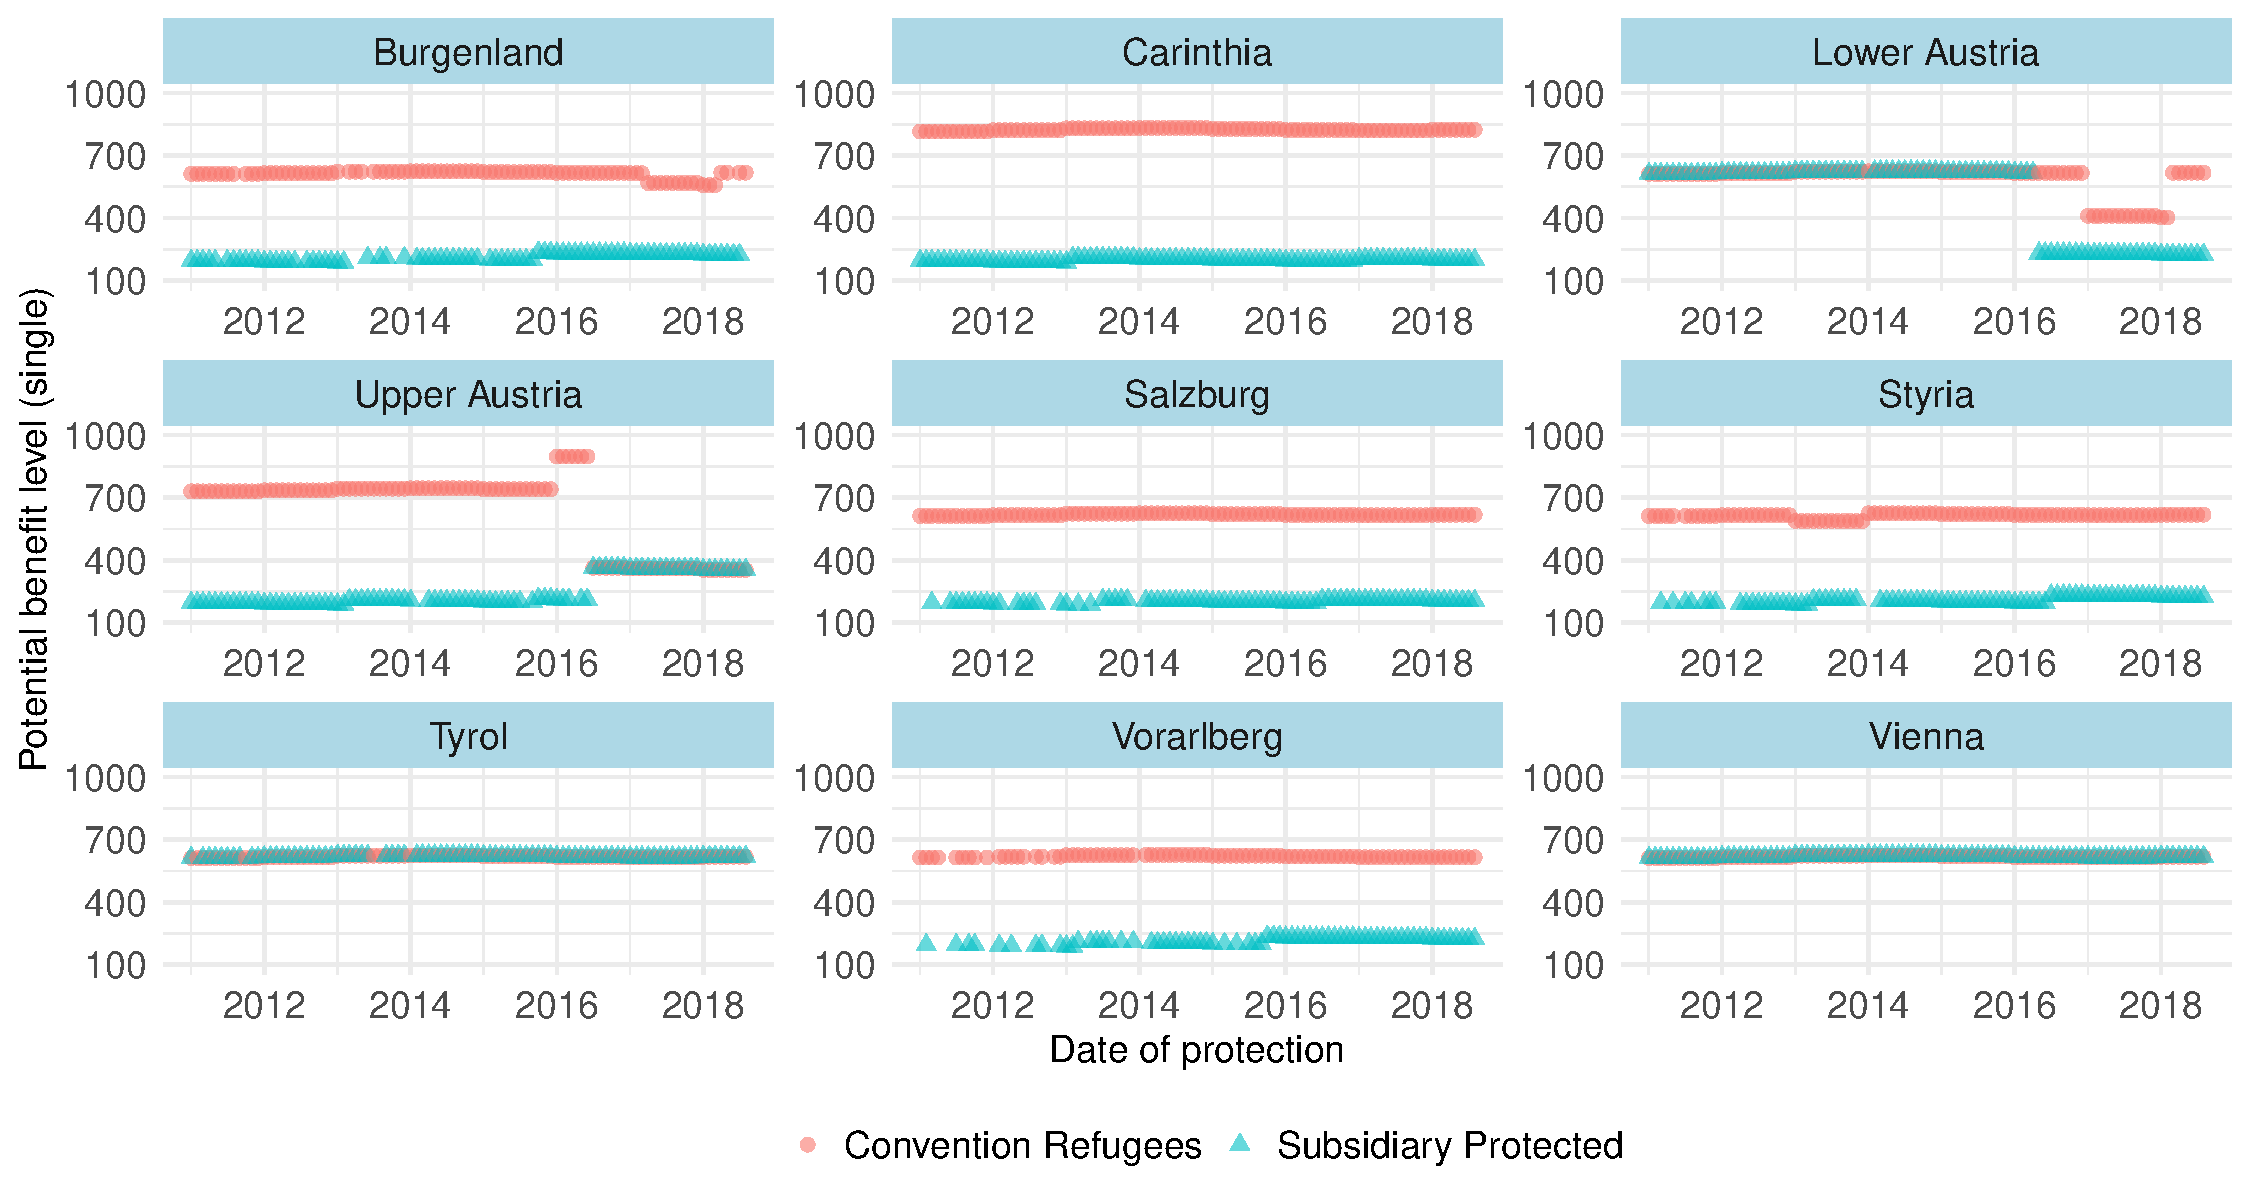
\includegraphics[scale=0.4]{figures/fig_ipbl.pdf}
    \end{center}
    \vspace{-0.7cm}
    \justify 
 		{\footnotesize 
 			\textit{Notes:}
    %\fignote{Notes: 
    The figure shows the amount of monthly benefits in euros (excluding housing benefits) for singles by federal state and type of protection.}
\end{figure}


\subsection*{Local economic conditions}

In addition to cross-state differences in benefit generosity, we exploit variation in the initial vacancy-to-unemployment ratio ($IVUR$) across districts over time.
Figure~\ref{fig:ivurmap} shows the average $IVUR$ during our period of analysis (2011--2018), providing a snapshot of the regional variation used in our analysis.

The graph shows that Vienna and districts in the eastern and southern states of the country display low average labor demand during this period.
 
These patterns are consistent with other labor market statistics at the state-level. For instance, Vienna exhibited the highest unemployment rate (8.4\%) in 2022 in Austria \citep{oecd_economy_aut}.

% \begin{figure}
%     \caption{Mean Vacancy-to-Unemployment Ratio by District}
%     \label{fig:ivurmap}
%     \begin{center}
%     \vspace{-0.5 cm}
%     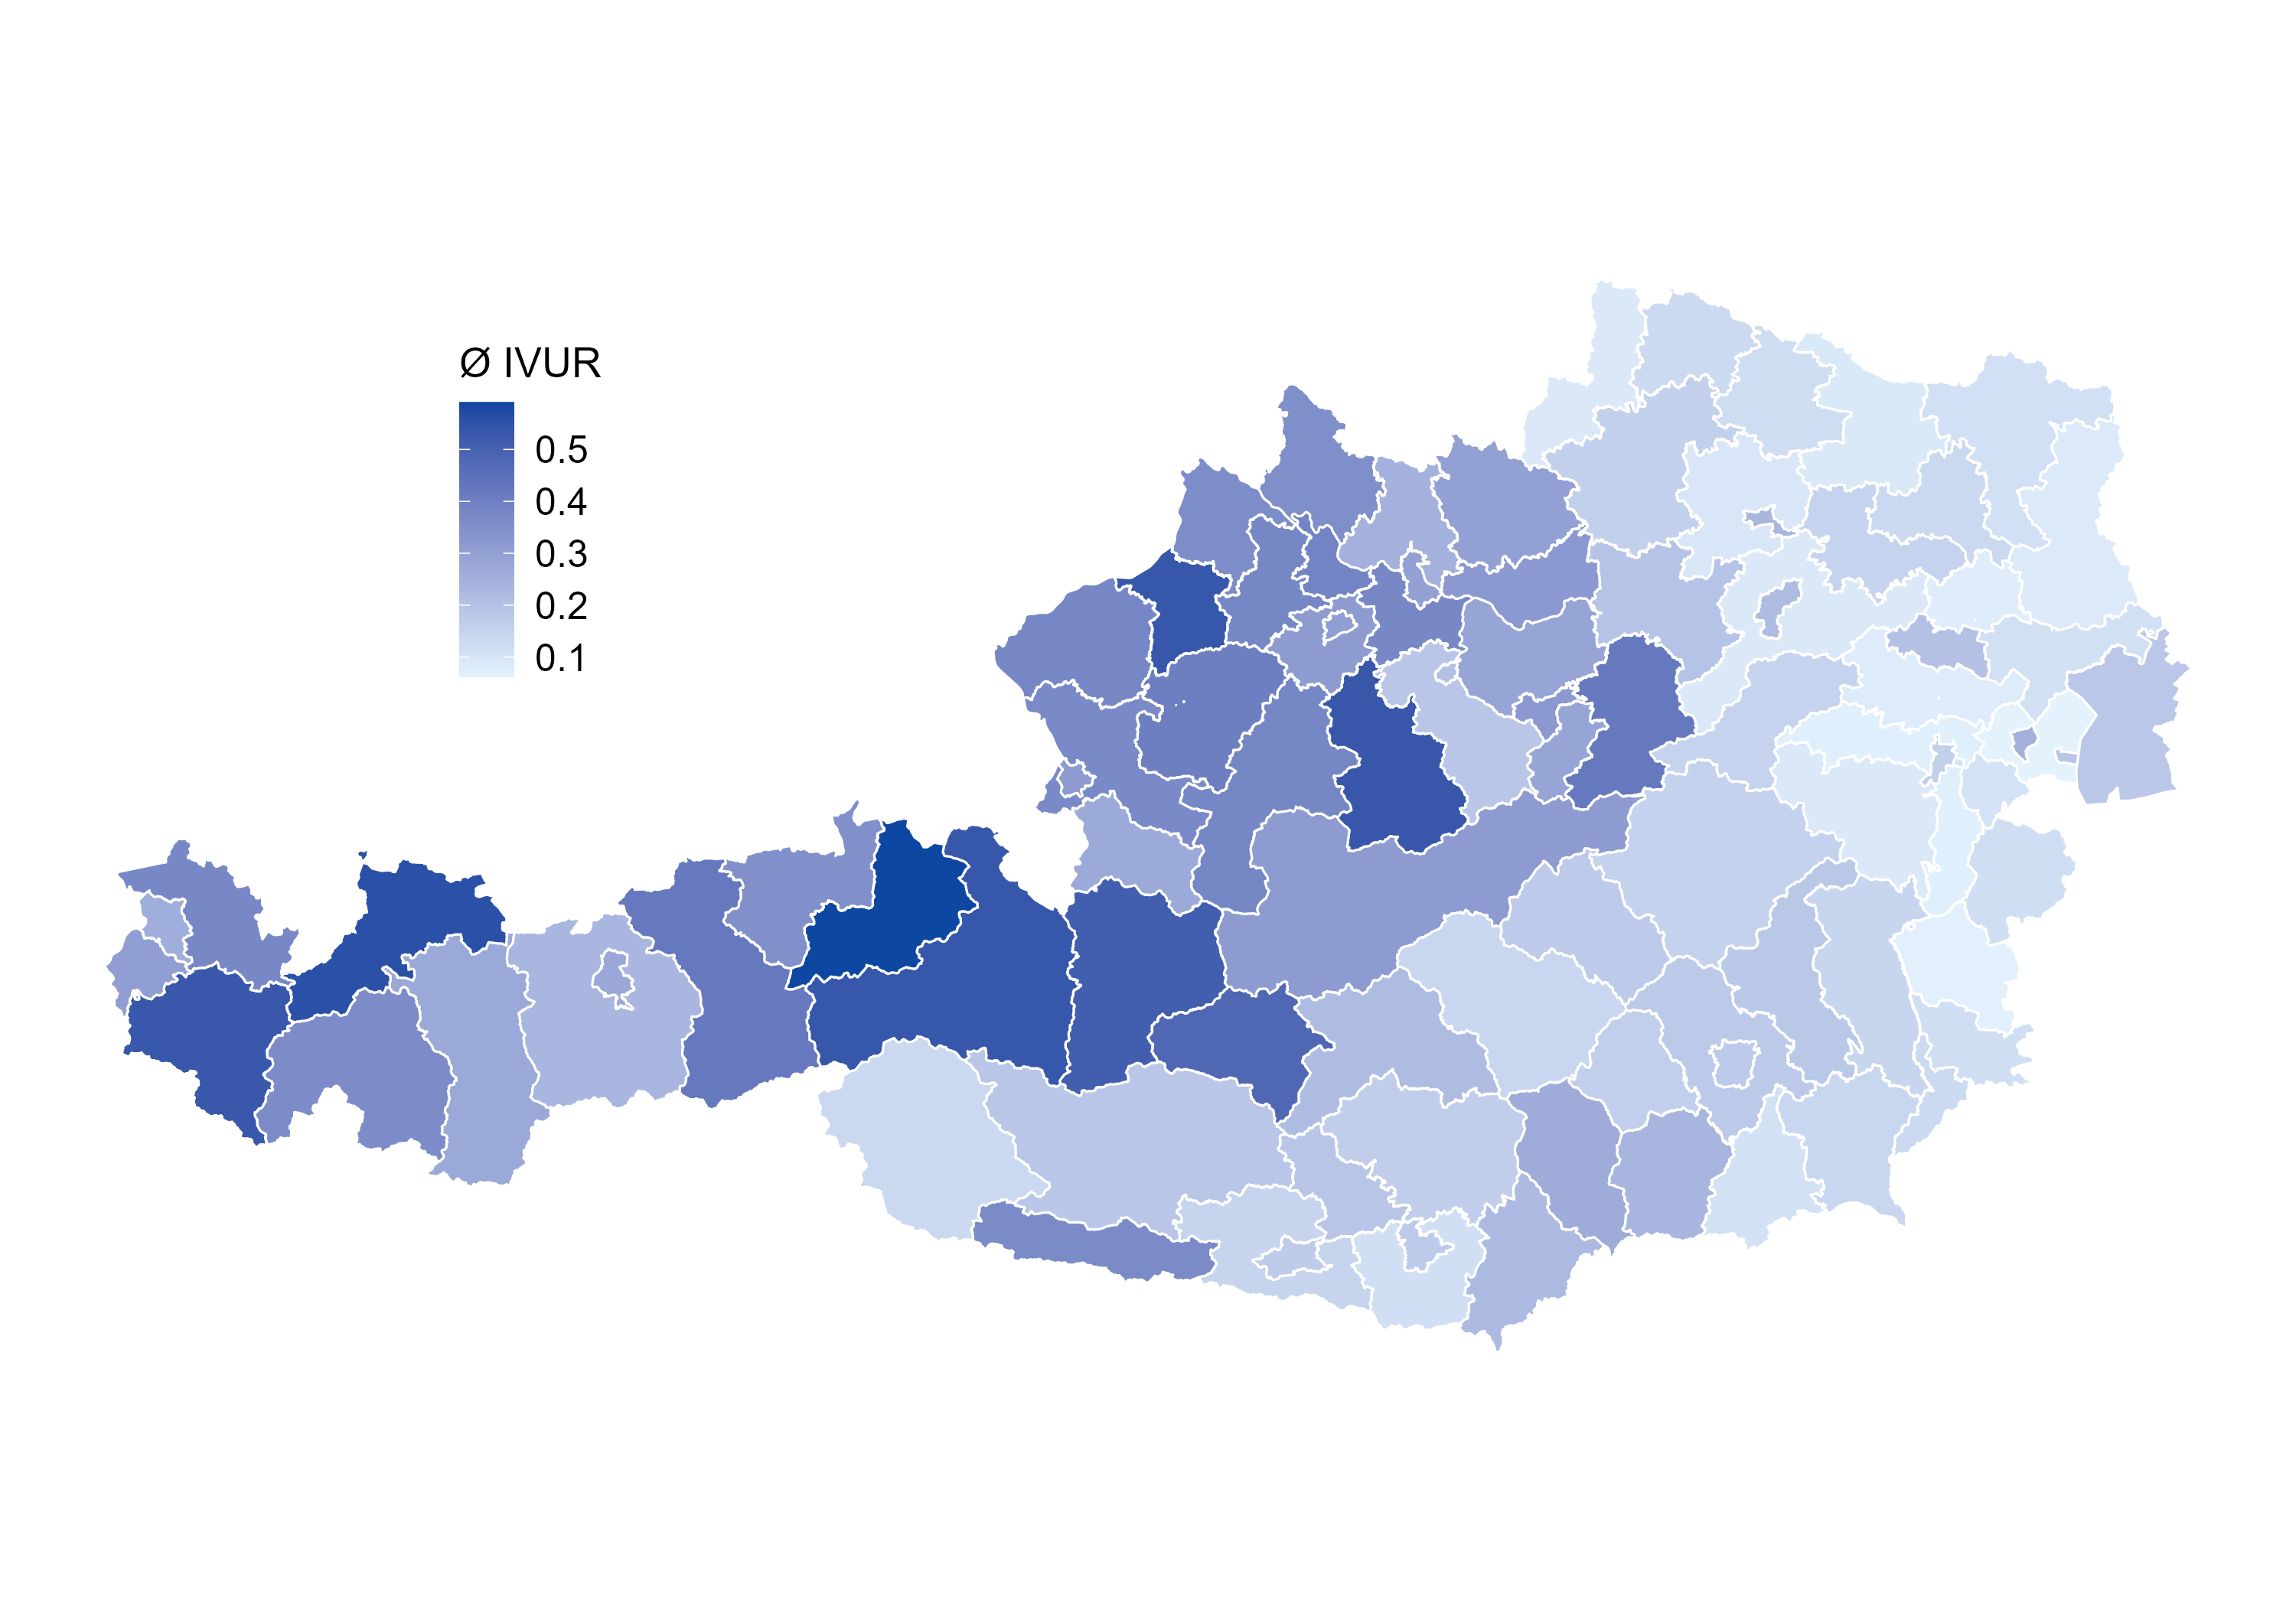
\includegraphics[scale=0.60]{figures/ivur_by_district_map.png}
%     \end{center}
%     \fignote{\footnotesize \textit{Notes:} 
% The map shows the mean vacancy-to-unemployment ratio ($IVUR$) by district, averaged across the period 2011–2018. District borders correspond to the NUTS 3 regional classification. Vienna is displayed as a single district.}
%     \vspace{-0.5 cm}
% \end{figure}

\begin{figure}
    \caption{Mean Vacancy-to-Unemployment Ratio by District}
    \label{fig:ivurmap}
    \begin{center}
    \vspace{-0.5 cm}
     \begin{tikzpicture}
    \node[anchor=south west,inner sep=0] (image) at (0,0) {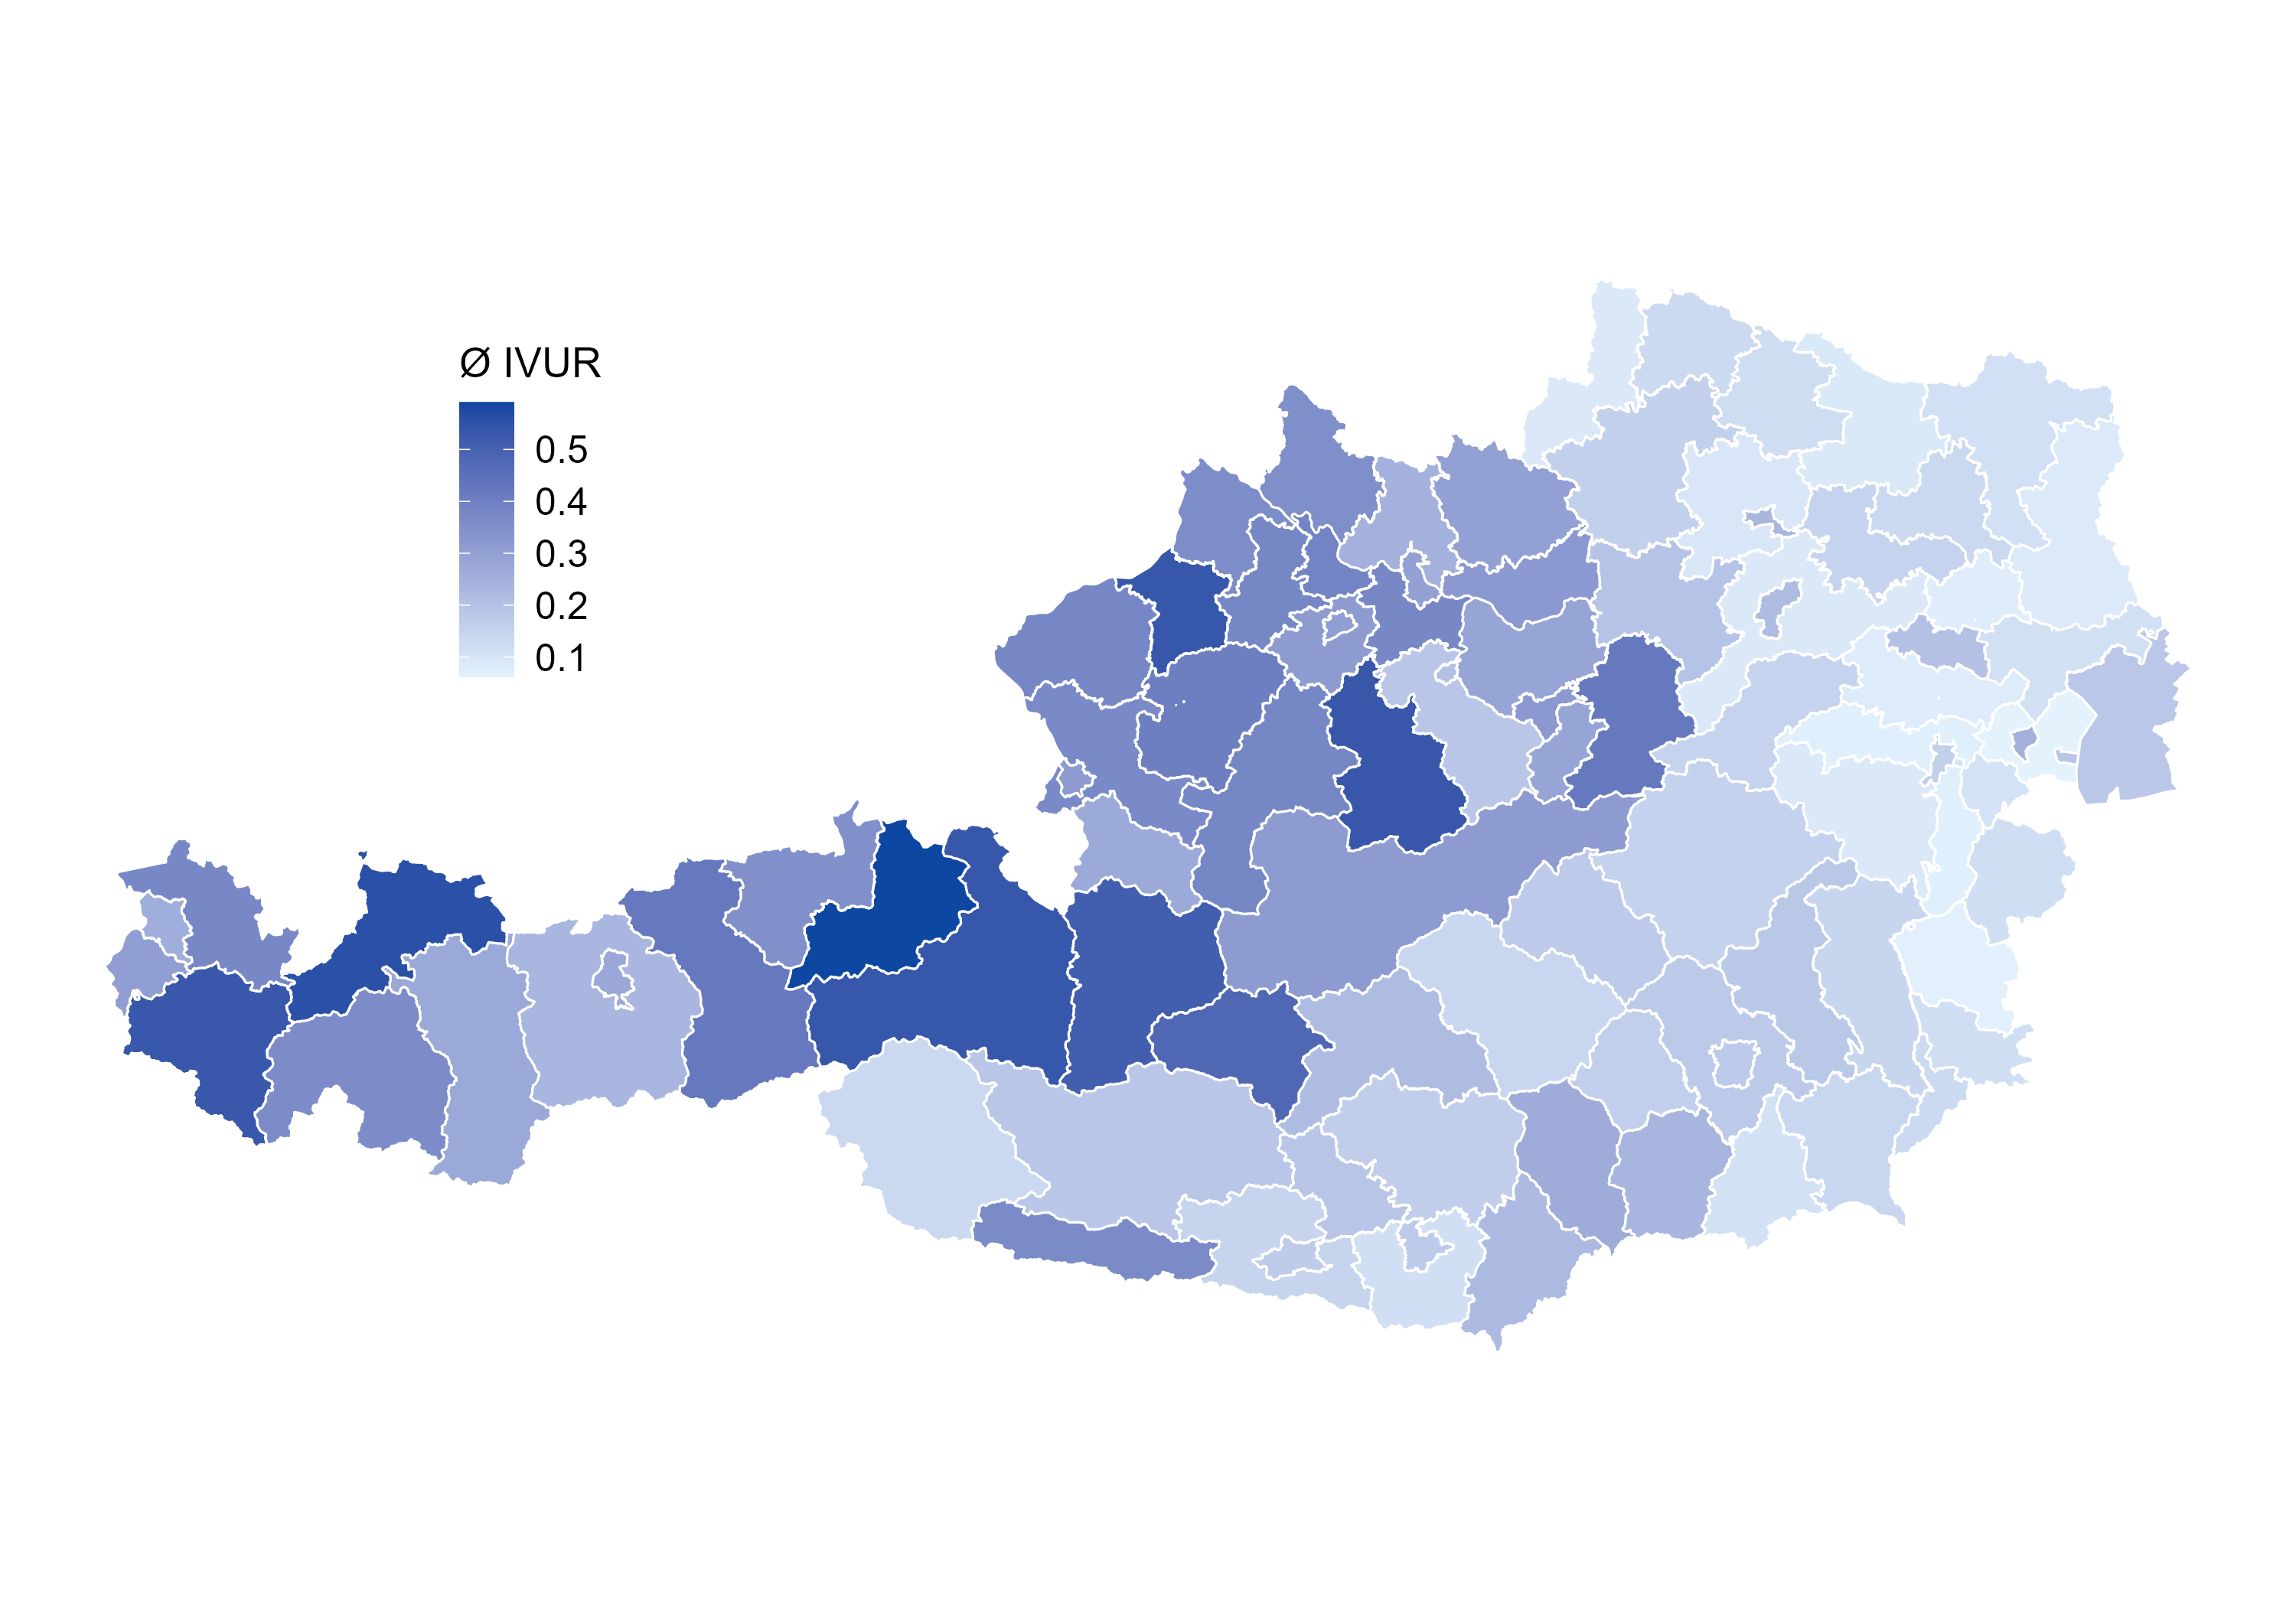
\includegraphics[width=\linewidth]{figures/ivur_by_district_map.png}};
    \begin{scope}[x={(image.south east)},y={(image.north west)}]
      % Arrow pointing to a location (x, y) in relative coordinates (0 to 1)
      \draw[<-, red, thick] (0.87, 0.63) -- (0.92, 0.68) node[above] {Vienna};
    \end{scope}
  \end{tikzpicture}
    \end{center}
    \fignote{\footnotesize \textit{Notes:} 
The map shows the mean vacancy-to-unemployment ratio ($IVUR$) by district, averaged across the period 2011–2018. District borders correspond to the NUTS 3 regional classification. Vienna is displayed as a single district.}
    \vspace{-0.5 cm}
\end{figure}

%\textbf{ADD SOME STATISTICS ON INFLOWS; COMPOSITION BY GENDER/FAMILY STATUS}



\FloatBarrier
%%%%%%%%%%%%%%%%%%%%%%%%%%%%%%%%%%%%%%%%%%%%%%%%%%%%%%%%%%%%%%%%%%%%%%%%%%%%%%%%%%%%%%%%%%%%%%%%%%%%%%%%%%%%
%%%%%%%%%%%%%%%%%%%%%%%%%%%%%%%%%% DATA   %%%%%%%%%%%%%%%%%%%%%%%%%%%%%%%%%%%%%%%%%%%%%%%%%%%%%%%%%%%%%%%%%
%%%%%%%%%%%%%%%%%%%%%%%%%%%%%%%%%%%%%%%%%%%%%%%%%%%%%%%%%%%%%%%%%%%%%%%%%%%%%%%%%%%%%%%%%%%%%%%%%%%%%%%%%%%%

\section{Data and Descriptive Statistics} \label{sec:dataoob}

\subsection{Data sources and sample} 
We use administrative data from the Austrian Social Security Database (ASSD), which covers all social insurance episodes and provides information on demographics, employment sectors, labor income, and spells of employment and unemployment. We augment the ASSD with variables from the Federal Ministry of Labor and Economy (BMAW), including protection type, asylum date, participation in educational programs, language proficiency, marital status, residency ZIP codes, basic income support, education level, previous and desired professions. This supplementary data covers all individuals granted protection status and registered with the Austrian Public Employment Service (PES) at any point in time. Although registration at the PES is voluntary, access to the social benefits linked to registration encourages it. In Appendix~\ref{subsec:pes_selection}, we test whether the number of refugees in our data, as a share of all individuals from those countries of origin in a district, correlates with our main explanatory variables, which is not the case.  %Still, we address potential sample selection biases in Section~\ref{identification}.

Asylum-seekers are granted special health insurance upon arrival, designated as ``O4'' or ``OE'' in the ASSD, signaling coverage under basic subsistence support. This unique classification enables the precise identification of asylum-seekers, distinguishing them from recipients of other insurance types. It also allows us to see whether subsidiary-protected individuals still receive this form of welfare benefits after being granted protection.

Our analysis encompasses all refugees granted protection under the Geneva Convention or subsidiary protection between January 2011 and August 2018.\footnote{The selection of 2011 as the starting point is due to improved data quality from this year onwards. The cutoff in August 2018 allows for a five-year observation period following the granting of protection status.} We focus on individuals aged 18 to 60 at the time of immigration, excluding those who were granted protection status on the day of arrival, indicative of family reunification. We further exclude refugees for whom calculating treatment variables was impractical,\footnote{In a few districts, the $IVUR$ could not be computed for certain observations during the early years of our observation period due to official zeroes in the unemployment count.} and individuals receiving protection more than three years after arrival.\footnote{We conduct robustness exercises with different sample restrictions in Section~\ref{subsec:robustnessoob}.}

Our final sample consists of 41,212 refugees, among whom 39,694 maintained active insurance coverage for a minimum of five years post-protection. In Section~\ref{no_insurance} of the Appendix, we examine the impact of our treatment variables on the probability of continuous insurance coverage over this five-year span. Finding no significant influence, we consequently limit our further analysis exclusively to those individuals who can be observed until the end of the five-year period.

Additionally, we enhance our dataset with detailed municipality characteristics from Statistics Austria and utilize the ASSD to ascertain the number of vacancies and unemployed individuals at the district level.


\subsection{Treatment variables}

\vspace{0.3cm}
\textbf{Initial vacancy-to-unemployment ratio \textit{(IVUR).}} \hspace{0.5cm} We characterize labor market tightness at the time of protection status receipt through the initial vacancy-to-unemployment ratio ($IVUR$), utilizing aggregated monthly data on registered unemployment and vacancies at the municipality level from the ASSD. The $IVUR$ is defined as follows:

\begin{equation}
\label{eq:IVUR}
IVUR_{d_0,t_0} = \frac{\sum_{t=0}^{2} \text{open positions}_{d_0, t}}{\sum_{t=0}^{2}\text{unemployed individuals}_{d_0, t}}
\end{equation}

This ratio is calculated by dividing the sum of open positions by the sum of unemployed individuals within a regional entity during the first three months following protection status receipt. $t_0$ refers to the month of receiving protection. $d_0$ refers to the district of residence when receiving protection. We choose political districts as they roughly align with labor markets.%\footnote{In Appendix XX, we investigate alternative regional aggregations and find that results are highly robust. (TO BE INCLUDED)}


\vspace{0.5cm}
\noindent\textbf{Initial Potential Benefit Level \textit{(IPBL).}} \hspace{0.5cm} Using the information on benefit levels introduced in Section~\ref{sec:background}, we define the Initial Potential Benefit Level ($IPBL$) as follows:

\begin{equation}
\label{eq:IPBL}
IPBL_{f,p,s_0,t_0} = \frac{PB_{f,p,s_0,t_0}}{1000}
\end{equation}

The $IPBL$ measures the monthly benefits available to a refugee with no other income or wealth. It depends on family status $f$,\footnote{We determine family benefit eligibility if a person's child is insured in Austria or if there is a partnership status with another asylum-seeker and at least one dependent child co-insured in Austria at the time of protection receipt. This is different from our family arrival variable used to define the arrival groups in our identification strategy, where we consider asylum-seekers who arrive in Austria on the same date.} type of protection $p$, state of residence at the time of protection $s_0$, and the date of protection $t_0$. We present $IPBL$ in units of 1,000 euro to facilitate a clearer graphical presentation of our findings. Consequently, $IPBL$ varies across federal states, protection statuses, family statuses, and over time, reflecting a sequence of policy reforms. A caveat is that our measure of benefit eligibility is imperfect, not covering other forms of benefits and only approximating the benefits for families. However, variation induced by the reforms should be captured very well. A second caveat is that $IPBL$ measures \emph{potential} rather than \emph{received} benefits. Refugees in private accommodation are directly affected by the cash component captured by $IPBL$, while refugees in organized accommodation receive most support in-kind and are only indirectly exposed---through the changed value of moving to private accommodation. As we do not observe accommodation type at the individual level, the $IPBL$ coefficients in Section~\ref{sec:results} average over both groups. We return to the implications for interpretation in Section~\ref{sec:discussion}.

Importantly, both $IVUR$ and $IPBL$ are assigned to each individual upon the granting of protection and remain unchanged thereafter. These indicators reflect the labor market tightness and the welfare benefits system that an asylum-seeker is subject to at the moment of initial authorization to enter the labor market and to move within Austria. Later changes in these variables due to relocation, amendments to benefit rules, or economic conditions are not considered as they are no longer assigned exogenously.

\subsection{Outcomes}

We examine three categories of outcomes at the individual level: labor market integration, mobility, and social support. %, utilizing administrative records from the social security agency and the PES. 
We express each metric on a monthly basis, with time standardized relative to the month of protection receipt. Labor market performance encompasses a) an indicator for being employed\footnote{Employment is defined as any employment spell subject to social insurance contributions.}, b) being in marginal employment\footnote{Marginal employments are employment spells with earnings below the marginal earnings threshold (€406 in 2015).}, c) monthly real labor earnings, and d) logged real monthly wage income\footnote{The earnings used to calculate real labor earnings and logged real monthly wage income are reported as pre-insurance, pre-tax gross income for each employer-employee relationship. For employment spells before 2019, earnings were reported annually, while after 2019, they have been reported on a monthly basis. We calculated average daily earnings for each employment contract and summed them up in cases of multiple simultaneous spells.}. For mobility, we track whether a refugee remains in the same state as when protection was granted and whether they reside in Vienna, specifically for those initially located in a different federal state. The mobility measure is based on the contact address available to the Social Security Administration. 
Social support metrics include a) receipt of any Public Employment Service (PES) support within a month, such as language courses, job training, or counseling, and b) receipt of any welfare benefits, and separated by basic needs support and basic subsistence support sources. Additionally, an active insurance spell serves as a proxy for a refugee's presence in Austria.\footnote{Our focus on individuals who received protection makes it rather unlikely that individuals switch to an informal status and remain in Austria, which would be an alternative explanation for an end to insurance in Austria.}

\FloatBarrier


\subsection{Descriptives}

Table~\ref{tab:summarystatistics} presents the summary statistics for our analysis sample, which consists of 39,694 individuals. Among these, 31,597 are Convention refugees, and 8,097 have subsidiary protection status. Two-thirds of refugees (64.7\%) are male, with an average age of 30.49 years at the time of immigration. More than half of the sample, 54.6\%, originates from Syria, followed by significant populations from Afghanistan (18.5\%), Iraq (7.8\%), and Iran (7.3\%). A substantial portion, 59.6\%, exhibits limited German language proficiency (A1/A2 level), and 69.2\% possess only primary education or lack it entirely. Noteworthy disparities exist between Convention refugees and subsidiary-protected individuals regarding their countries of origin, the duration of asylum processes (12.1 months for Convention refugees versus 15.9 months for those with subsidiary protection), and their eligibility for family benefits\footnote{We define eligibility for family benefits when receiving protection for refugees as applicable to those who are co-insured or provide co-insurance--- through a partnership or a parent-child relationship---to another individual who has been registered as a refugee in Austria on or before the date of protection.} (35.9\% versus 24\%). $IVUR$ is similar across groups, but on average, the $IPBL$ for subsidiary-protected individuals is €308 lower due to a lower likelihood of being eligible for family benefits and generally less generous benefits for this group (see Section~\ref{sec:background}).

The final panel of the table details outcomes measured in the 12\textsuperscript{th} month post-protection. Around 95\% have an active insurance spell. The employment rate is 11.3\% with mean monthly earnings of €203. Subsidiary-protected refugees do slightly better than Convention refugees on both metrics. 71\% of Convention and 61\% of subsidiary-protected refugees still live in the same state as initially assigned to. Given the low labor market integration, dependence on welfare benefits is high; 75\% receive some form of benefits, and approximately 38\% receive support from the PES.

\begin{table}
    \caption{Summary statistics}
    \label{tab:summarystatistics}
    \begin{threeparttable}
        \begin{small}
          %  \resizebox{\linewidth}{!}{%
                \begin{tabular}{lcccc}
                    %\expandableinput
                    \begin{tabular}{lccc}
\toprule
 & Convention refugee & Subsidiary-protected & Total \\
\midrule
\multicolumn{1}{l}{} & \multicolumn{3}{c}{Time-invariant characteristics} \\
Gender (female=0) & 0.63 (0.48) & 0.70 (0.46) & 0.65 (0.48) \\
Age at immigration & 30.75 (9.17) & 29.49 (9.46) & 30.49 (9.25) \\
Origin country & & & \\
\quad Afghanistan & 4440 (14.1\%) & 2903 (35.9\%) & 7343 (18.5\%) \\
\quad Iran & 2779 (8.8\%) & 124 (1.5\%) & 2903 (7.3\%) \\
\quad Iraq & 1806 (5.7\%) & 1287 (15.9\%) & 3093 (7.8\%) \\
\quad Other & 1623 (5.1\%) & 639 (7.9\%) & 2262 (5.7\%) \\
\quad Russia & 433 (1.4\%) & 158 (2.0\%) & 591 (1.5\%) \\
\quad Somalia & 631 (2.0\%) & 1190 (14.7\%) & 1821 (4.6\%) \\
\quad Syria & 19885 (62.9\%) & 1796 (22.2\%) & 21681 (54.6\%) \\
Duration asylum process & 12.08 (9.02) & 15.90 (9.50) & 12.86 (9.25) \\
German skill level & & & \\
\quad A & 18786 (59.5\%) & 4872 (60.2\%) & 23658 (59.6\%) \\
\quad B/C & 6019 (19.0\%) & 1258 (15.5\%) & 7277 (18.3\%) \\
\quad unknown & 6792 (21.5\%) & 1967 (24.3\%) & 8759 (22.1\%) \\
Education level & & & \\
\quad primary & 21344 (67.6\%) & 6122 (75.6\%) & 27466 (69.2\%) \\
\quad secondary & 4469 (14.1\%) & 640 (7.9\%) & 5109 (12.9\%) \\
\quad tertiary & 1913 (6.1\%) & 219 (2.7\%) & 2132 (5.4\%) \\
\quad unknown & 3871 (12.3\%) & 1116 (13.8\%) & 4987 (12.6\%) \\
Family benefit eligibility & 0.36 (0.48) & 0.24 (0.43) & 0.34 (0.47) \\
\multicolumn{1}{l}{} & \multicolumn{3}{c}{Initial local conditions} \\
IVUR & 0.19 (0.15) & 0.20 (0.16) & 0.19 (0.15) \\
IPBL (in €1,000) & 0.83 (0.29) & 0.52 (0.29) & 0.76 (0.32) \\
\multicolumn{1}{l}{} & \multicolumn{3}{c}{Outcomes in month twelve} \\
No Austrian insurance & 0.06 (0.23) & 0.03 (0.16) & 0.05 (0.22) \\
In employment & 0.10 (0.30) & 0.17 (0.37) & 0.11 (0.32) \\
Monthly real earnings & 180.27 (551.53) & 292.51 (663.54) & 203.16 (577.92) \\
In marginal employment & 0.03 (0.18) & 0.03 (0.18) & 0.03 (0.18) \\
Residency in initial state & 0.71 (0.45) & 0.61 (0.49) & 0.69 (0.46) \\
Residency in Vienna & 0.51 (0.50) & 0.58 (0.49) & 0.52 (0.50) \\
PES services & 0.38 (0.48) & 0.39 (0.49) & 0.38 (0.49) \\
Receiving welfare benefits & 0.76 (0.43) & 0.74 (0.44) & 0.75 (0.43) \\
\midrule
Observations & N=31597 & N=8097 & N=39694 \\
\bottomrule
\end{tabular}
                \end{tabular}
        %    }
        \end{small}
       % \vspace{-1em}
        \begin{tablenotes}
           % \parbox[t]{\textwidth}{%  % Set a strict width to the text width
           \footnotesize
                \item {\textit{Notes:} The table reports means and standard deviations (in brackets) for continuous and binary variables. The number of observations and the percentage within groups are reported for categorical variables. Time-varying (outcome) variables are reported for the 12\textsuperscript{th} month after protection was received. The sample is restricted to refugees who received protection between January 2011 and August 2018, who were between 18 and 60 years old at the time of immigration and whose asylum process lasted longer than a day but less than three years, and where full data is available for 60 months after the date of protection. Family benefit eligibility is an indicator equal to one if children who are co-insured with this person or their partner are registered in Austria at the time of receiving protection. Duration of asylum process is denoted in months, earnings are denoted in real 2015 euros, and IPBL is denominated in €1,000 (real 2015 values) to match the convention used throughout the regression analysis and all figures.}
   %         }
        \end{tablenotes}
    \end{threeparttable}
\end{table}

Figure~\ref{fig:descriptive_outcomes_main} shows how the employment rate (left) and the share of refugees who remain in the initial state (right) evolve from the moment of receiving protection. The employment rate starts from near zero at the time of protection. For men, it rises steadily and reaches about 60\% after five years. For women, the employment rate is less than 20\% after five years. The other notable aspect is high mobility rates immediately after receiving protection. Within six months, a quarter of refugees have moved to another state. Mobility is higher for men than for women. Figure~\ref{fig:descriptive_outcomes_appendix} in the Appendix shows the evolution of other outcome variables by gender over time.



\begin{figure} 
    \caption{Share of refugees in employment and residency in initial state by time since receiving protection} %\\ by months since protection was received.}
    \label{fig:descriptive_outcomes_main}
    \begin{center}        
        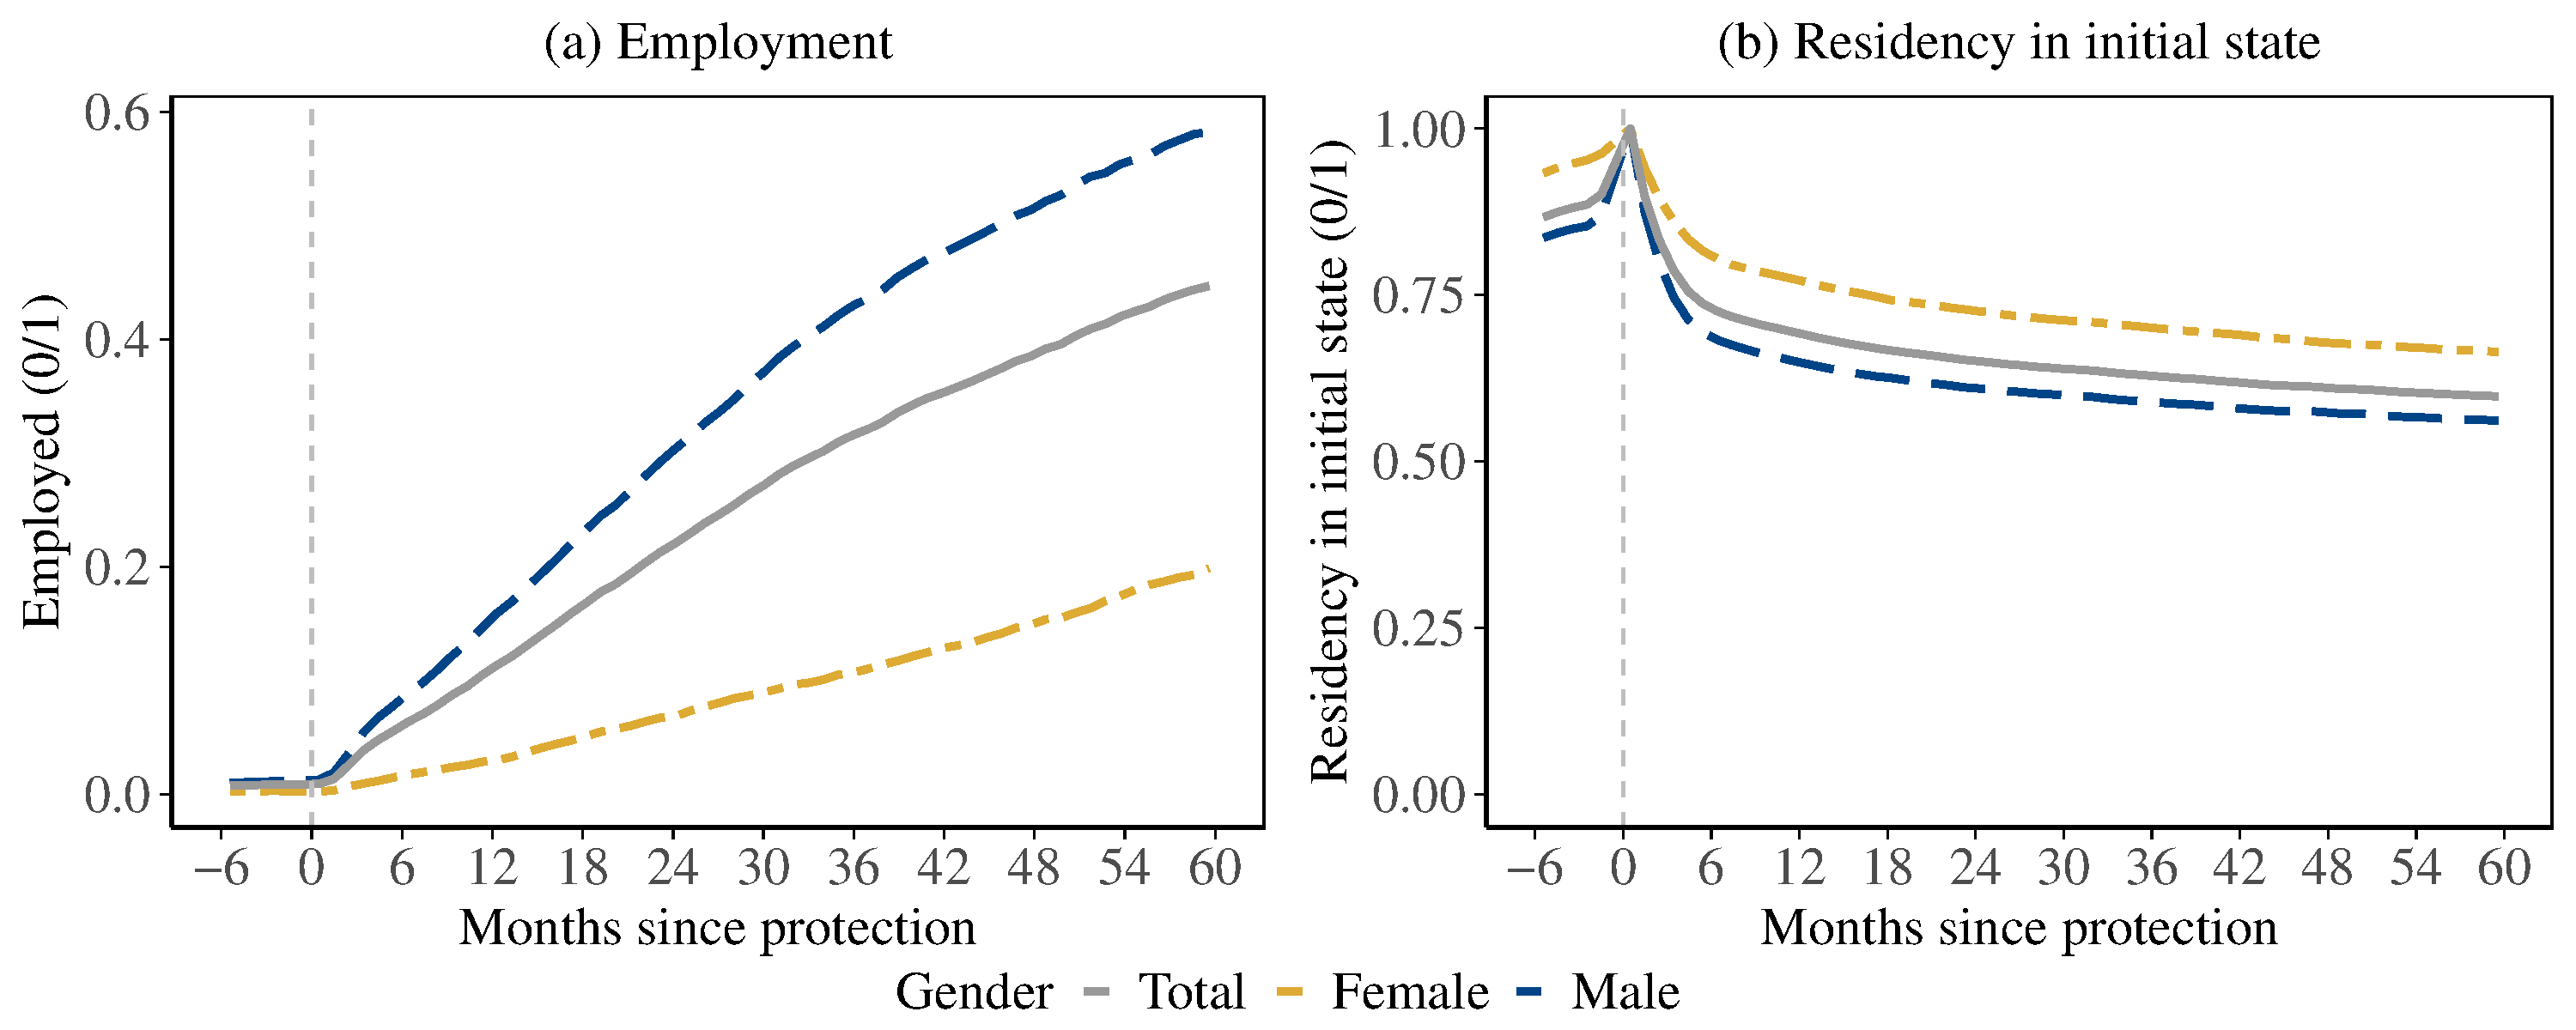
\includegraphics[scale=0.3]{figures/fig_descriptive_outcomes_main.pdf}
    \end{center}
% \\
       \justify 
 	{\footnotesize 
 		\textit{Notes:}   
%\fignote{Notes: 
The figure shows the share of employed refugees and of refugees who remained in their initial state by months since protection and gender. The x-axis shows the months since receiving protection. The y-axis displays the shares of refugees in (a) employment or (b) residing in the state of protection (initial state).}
\end{figure}

Mobility patterns after receiving protection vary substantially between federal states (see Figure~\ref{fig:movermatrix}). In Vienna, 96\% of refugees remain, while only 26\% do so in Burgenland, the other end of the distribution. The overwhelming majority of individuals who move between federal states move to Vienna. Twelve months after protection, 90 or more percent of all refugees are either in their initial states or in Vienna. The other states play only a marginal role as destinations for internal mobility.

\begin{figure} 
    \caption{Residence of refugees twelve months after receiving protection by initial state} %\\ by months since protection was received.}
    \label{fig:movermatrix}
    \begin{center}               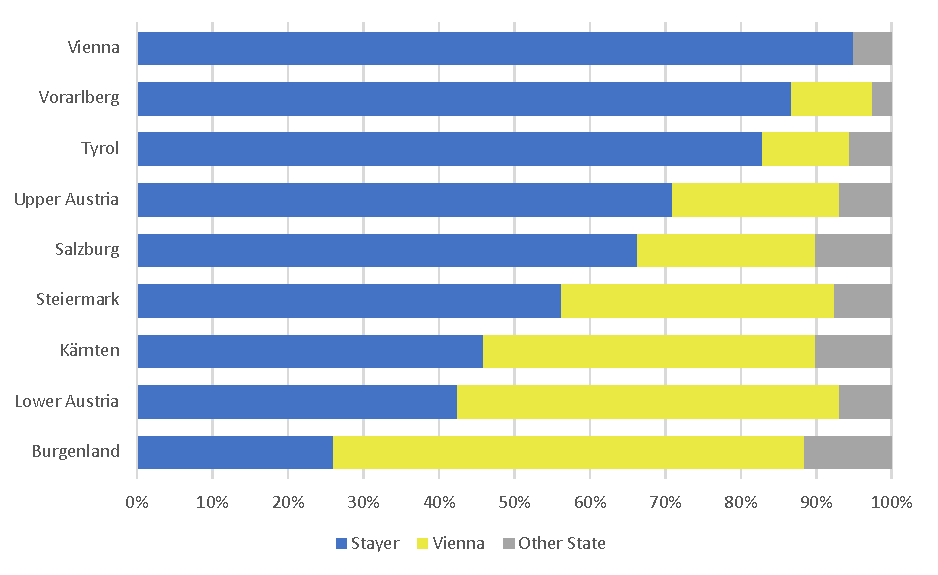
\includegraphics[width=0.7\textwidth]{figures/fig_movermatrix.pdf}
    \end{center}
%\fignote{Notes: 
  \justify 
 	{\footnotesize 
 		\textit{Notes:} The figure shows the state of residence of refugees twelve months after receiving protection. Stayers remain in the initial state (blue). Yellow bars indicate the shares that move from another state to Vienna. Gray bars indicate the shares that move to a state other than Vienna. %XXX: CLARIFY WHETHER THIS IS THE SAME SAMPLE AS IN PREVIOUS FIGURE
}
\end{figure}

Vienna is not only an attractive destination among refugees but also among other migrants. While 22\% of the Austrian population live in Vienna, this share is about 40\% among foreigners. On the other end, Burgenland, with 3.3\% of the population, only hosts 2\% of foreigners in Austria \citep{statistikaustria_2024}.
% \begin{figure}[htbp]
%     \centering
%      \caption{Evolution of positive decisions from BMI and our proxy for family reunified members, 2016-2022, quarterly}
%     \includegraphics[width=0.8\textwidth]{bmi_assd6m_en.png}
%        \label{fig:bmiassd}
% \end{figure}


\FloatBarrier

%%%%%%%%%%%%%%%%%%%%%%%%%%%%%%%%%%%%%%%%%%%%%%%%%%%%%%%%%%%%%%%%%%%%%%%%%%%%%%%%%%%%%%%%%%%%%%%%%%%%%%%%%%%%
%%%%%%%%%%%%%%%%%%%%%%%%%%%%%%%%%% METHOD   %%%%%%%%%%%%%%%%%%%%%%%%%%%%%%%%%%%%%%%%%%%%%%%%%%%%%%%%%%%%%%%%%
%%%%%%%%%%%%%%%%%%%%%%%%%%%%%%%%%%%%%%%%%%%%%%%%%%%%%%%%%%%%%%%%%%%%%%%%%%%%%%%%%%%%%%%%%%%%%%%%%%%%%%%%%%%%
\FloatBarrier
\section{Empirical Approach} \label{sec:empirics}

In an ideal experiment to understand the impact of two treatments and their interaction, one would randomize the receipt of those two treatments. However, such randomization is conceptually not feasible in our context. While it is conceivable to assign benefit generosity, labor demand, driven by the economy's evolution, cannot be manipulated in the same manner. Therefore, we must conceptualize treatment assignments differently. Rather than assigning treatments to individuals, we allocate individuals to treatments based on their location, timing, protection status and family status. Each combination of place, time, and status cells comes with values for the treatment variables, $IVUR$ and $IPBL$.

Approaching identification from this angle requires separately thinking about two levels of identifying assumptions. First, are individuals exogenously assigned to cells? Second, are there other characteristics of these cells that are correlated with the value of the treatment variables also affecting the outcomes and thus confounding the analysis?

Subsequently, we describe our empirical strategy that seeks to address both levels of the identification problem. We start with a description of the econometric specification and subsequently explain how this specification is linked to our identification problem.

\subsection{Econometric specification} \label{sec:specification}

The essence of our empirical strategy is to exploit exogenous variation in the initial local labor market conditions and welfare benefit generosity that refugees face at the time and place of protection. For each individual $i$, we denote the time of protection as $t^0(i)$, the district of residence at protection as $d^0(i)$, and the state at protection as $s^0(i)$. Both the initial vacancy-to-unemployment ratio ($IVUR_{d^0(i), m^0(i)}$) and the initial potential benefit level ($IPBL_{p(i), f(i), s^0(i), m^0(i)}$) are measured for the district or state and month of protection. Here, $p(i)$ denotes protection type, $f(i)$ family status, and $m^0(i)$ the calendar month of protection. 

Outcomes $Y_{i d(t) t}$ are measured at time $t$ for the location where the individual resides at $t$, which may differ from the initial location. All fixed effects for the month-year of protection, arrival group, and district of residence at protection are allowed to vary by the outcome period. This specification ensures that all group and contextual adjustments are flexibly modeled for each time horizon. Crucially, $IVUR$ and $IPBL$ are fixed at the protection-date values for the entire 60-month outcome window, so $\beta_{1,t}$ and $\beta_{2,t}$ at long horizons identify the effect of \emph{initial} conditions on later outcomes, not the effect of the contemporaneous labor market or benefit regime that a relocated refugee may no longer face.

Formally, the primary specification estimated for each outcome period $t$ is:

%\begin{equation}
\begin{align}\label{eq:main}
Y_{i d(t) t} =\ & \alpha_t + \beta_{1,t}\ IVUR_{d^0(i), m^0(i)} + \beta_{2,t}\ IPBL_{p(i), f(i), s^0(i), m^0(i)} \notag \\
& +\ \gamma_{m^0(i), t} + \delta_{g(i), t} + \eta_{d^0(i), t} + X_i'\Gamma_t + \epsilon_{i d(t) t}
\end{align}
%\end{equation}

where $Y_{i d(t) t}$ denotes the outcome for individual $i$ observed at time $t$, in the current district $d(t)$. $IVUR_{d^0(i), m^0(i)}$ and $IPBL_{p(i), f(i), s^0(i), m^0(i)}$ capture initial conditions at the time and place of protection. $\gamma_{m^0(i), t}$, $\delta_{g(i), t}$, and $\eta_{d^0(i), t}$ denote fixed effects for the month-year of protection, arrival group, and district at time of protection, all specific to outcome period $t$. $X_i$ is a vector of time-invariant individual controls, including age at immigration and its square, type of protection status, country of origin, and eligibility for family benefits, and $\epsilon_{i d(t) t}$ denotes the error term. 

\subsection{Identification strategy} \label{identification}

Identification of the $IVUR$ and $IPBL$ effects in Equation~\ref{eq:main} rests on two conditional independence assumptions. Conditional on arrival-group, month-year-of-protection, and district-of-protection fixed effects ($\delta_{g(i),t}$, $\gamma_{m^0(i),t}$, $\eta_{d^0(i),t}$) together with our individual controls $X_i$, we assume that (i) $IVUR_{d^0(i), m^0(i)}$ is mean-independent of the outcome residual, and (ii) the same holds for $IPBL_{p(i), f(i), s^0(i), m^0(i)}$. Sections~\ref{identification_cells} and~\ref{identification_treatments} justify these assumptions in turn.

\subsubsection{Assignment to location-time-protection status-cells} \label{identification_cells}

First, we consider the allocation of refugees to the districts where they reside when receiving protection. This is the district where they get access to the Austrian labor market and that determines under which state's welfare regime they initially fall. As explained in Section~\ref{sec:allocation}, municipalities might indicate preferences regarding the characteristics of asylum-seekers they can host. Thus, we expect systematic differences in the characteristics of refugees between municipalities. We address this issue by implementing arrival-group fixed effects $\delta_g$. Within groups of people of the same gender who arrived in Austria in the same quarter, were initially registered in the same state, and arrived alone or as a family, the assignment to municipalities depends on the next available housing unit at that point in time. Thus, within arrival groups, it is a haphazard process to determine which asylum-seeker goes to which municipality. Further, asylum-seekers are effectively banned from relocating to another state as they would lose benefits and are mostly unable to relocate within a state due to financial constraints.\footnote{The basic subsistence support usually provides housing in organized accommodations. In the case of independent relocation to private housing within the state, asylum-seekers only receive a small monthly compensation, which is usually insufficient to pay for rent.} Given these constraints, conditional on the arrival group, denoted as $\delta_{g}$ in our specifications, asylum-seekers find themselves quasi-randomly assigned to the district where they live when their protection is granted.

The duration until the asylum claim is processed primarily depends on the capacity of the bureaucracy and can barely be influenced by the asylum-seeker. Thus, the specific month-year in which protection is granted is also exogenous, conditional on the arrival group.

$IPBL$ also depends on protection type and family status. Both factors might directly influence our outcomes of interest. Thus, we condition on eligibility for family benefits and protection type to only compare individuals within the respective group.

In sum, asylum-seekers cannot select a district based on perceived labor market prospects or welfare benefits, nor determine the timing of receiving protection. Municipalities can only express preferences over broad characteristics, which is why we seek to make comparisons within arrival groups.

%Hence, any variation in IVURs and IPBLs should stem from local variations in labor market prospects or changes in the state's level of welfare benefits, independent of any choice a refugee might take during the asylum process. If this assumption holds, the $IVUR$ and $IPBL$ a refugee experiences at the date of being granted protection can be seen as random shocks, representing proxies for the local labor market conditions and the local welfare system, respectively.



\begin{table}
	\caption{Correlation of initial vacancy-to-unemployment ratio and initial potential benefit level with migrant characteristics}
	\label{tab:ivur_ipbl_balance}
 \centering
	\begin{threeparttable}
		\begin{small}
   \centering
			\begin{tabular}{lcccc}				
   
\centering
\begin{tabular}[t]{lcccc}
\toprule
& (1) & (2) & (3) & (4) \\
  & IVUR & IVUR  & IPBL & IPBL \\
\midrule
Asylum process duration & \num{0.045} & \num{0.353} & \num{0.286} & \num{0.447}\\
 & (\num{0.064}) & (\num{0.305}) & (\num{0.197}) & (\num{0.776})\\
Age at immigration & \num{-0.034} & \num{-0.013} & \num{0.178}*** & \num{0.118}*\\
 & (\num{0.031}) & (\num{0.026}) & (\num{0.068}) & (\num{0.066})\\\midrule
& \multicolumn{4}{c}{Education (reference category: Primary)}\\Secondary education & \num{-3.803}*** & \num{-1.849}* & \num{-4.909}* & \num{-4.257}*\\
 & (\num{1.443}) & (\num{1.084}) & (\num{2.626}) & (\num{2.431})\\
Tertiary education & \num{-2.981}** & \num{-1.512} & \num{-7.342}*** & \num{-7.276}***\\
 & (\num{1.424}) & (\num{1.040}) & (\num{2.689}) & (\num{2.279})\\
Unknown education & \num{-0.554} & \num{-0.155} & \num{3.192} & \num{2.315}\\
 & (\num{1.076}) & (\num{0.970}) & (\num{2.425}) & (\num{2.271})\\
\midrule
& \multicolumn{4}{c}{German skills (reference category: A)}\\B/C german skills & \num{-0.033} & \num{-0.525} & \num{-3.943}** & \num{-4.049}**\\
 & (\num{0.795}) & (\num{0.711}) & (\num{1.930}) & (\num{1.778})\\
Unknown german skills & \num{-0.612} & \num{0.127} & \num{-0.888} & \num{0.228}\\
 & (\num{0.710}) & (\num{0.638}) & (\num{2.004}) & (\num{1.743})\\
\midrule
& \multicolumn{4}{c}{Known Confounders IPBL}\\Convention refugee & \num{-1.601}* & \num{-0.560} & \num{242.678}*** & \num{239.790}***\\
 & (\num{0.942}) & (\num{0.901}) & (\num{27.504}) & (\num{27.982})\\
Family benefit eligibility & \num{2.199}** & \num{-1.146} & \num{560.072}*** & \num{564.161}***\\
 & (\num{0.968}) & (\num{0.842}) & (\num{5.759}) & (\num{5.247})\\
\midrule
District FE & X & X & X & X\\
Month and year FE & X & X & X & X\\
Country of origin FE & X & X & X & X\\
Arrival group FE &  & X &  & X\\
\midrule
N & \num{39694} & \num{39694} & \num{39694} & \num{39694}\\
\midrule
Wald-Test (p-value) IVUR & 0.8 & 0.997 & - & -\\
Wald-Test (p-value) IPBL & - & - & 0.594 & 0.802\\
\bottomrule
\end{tabular}


			\end{tabular}
		\end{small}
		\begin{tablenotes} 
			\begin{footnotesize}
				\begin{spacing}{1}
					\textit{Notes:} Coefficients from OLS regressions of the $IVUR$ and $IPBL$ at the month of protection on migrant characteristics as well as a full set of district-at-protection, year-month, and country-of-origin fixed effects. $IVUR$ and $IPBL$ are multiplied by 1000 for better depiction. Columns 2 and 4 also include arrival-group fixed effects. The Wald test statistics test the full models against a restricted model with i) only fixed effects for the $IVUR$ and ii) fixed effects and dummy variables indicating the type of protection and assumed family status at protection date. Standard errors are clustered at the state-year-of-protection level. */**/*** denote statistical significance at the 10/5/1 percent level.
				\end{spacing}
			\end{footnotesize}
		\end{tablenotes}
	\end{threeparttable}
\end{table}

While we cannot directly ascertain if asylum-seekers could self-select into specific districts or influence the duration of their asylum process, we can investigate if $IVUR$ and $IPBL$ correlate with individual characteristics.
We achieve this by regressing i) the district-level $IVUR$ and ii) the state-level $IPBL$ on district, month-year of protection, country of origin, and arrival group fixed effects. Additionally, we control for the type of protection and an indicator for family benefit eligibility, which are established confounders for the $IPBL$ since the $IPBL$ varies with protection type and family size.

Columns (1) and (3) of Table~\ref{tab:ivur_ipbl_balance} present the results without arrival group fixed effects, columns (2) and (4) with. All coefficients are close to zero and negligible in magnitude. For example, with arrival group fixed effects, individuals with secondary education face an $IVUR$ of 0.001849 smaller than individuals with primary education. This amounts to roughly one percent of a standard deviation of $IVUR$. Similarly, the coefficient for $IPBL$ suggests that individuals with secondary education face an $IPBL$ that is about four euros lower than individuals with primary education.

The overarching Wald tests do not reject the hypotheses that personal characteristics are uncorrelated to $IVUR$ and $IPBL$, with p-values in all specifications being at least 0.59.\footnote{For the $IVUR$, we contrast the model with all presented personal characteristics against the model with only fixed effects. For the $IPBL$, we compare the full model to one that includes only the fixed effects and the known confounders.} Overall, these results support our argument that the placement of asylum-seekers to districts is exogenous.

\subsubsection{Exogeneity of \textit{IVUR} and \textit{IPBL}} \label{identification_treatments}

Second, we consider a possible correlation between $IVUR$ and $IPBL$ and other local characteristics affecting refugees' labor market success. For example, regions with high $IVUR$ and $IPBL$ could also have a more welcoming civil society that helps refugees integrate better. To address this concern, we include district fixed effects $\eta_{d_0}$ that control for all time-constant regional characteristics with constant effects. Controlling for month-year of protection, fixed effects $\gamma_{t_0}$ holds constant all factors that influence all regions in the same way, such as national policy changes. Because $\eta_{d_0}$ absorbs each district's long-run average tightness, the $IVUR$ variation our specification exploits is by construction a within-district deviation: our coefficient $\beta_{1,t}$ identifies responses to transient tightness shocks at the moment of protection, not to differences in average labor-market quality across destinations.

Given these fixed effects, we deem it unlikely that $IVUR$ is confounded by other local factors influencing the outcome. The argument is less clear for $IPBL$. The welfare reforms, which drive most of the variation in benefit levels, might result from a broader change in attitudes towards refugees, which might also affect the outcomes. While we cannot fully rule out this possibility, we argue that we can sign the direction of the resulting bias for each outcome. Districts with higher $IPBL$ are likely to have more pro-refugee attitudes, which themselves may affect refugee outcomes. For the probability of remaining in the initial state, both channels operate in the same direction---pro-refugee attitudes and more generous benefits each encourage staying---so our estimate of the effect of benefits on staying reflects an upper bound (in absolute terms) on the causal effect. For employment, the channels operate in opposite directions: pro-refugee attitudes may raise refugee employment through reduced employer discrimination, partially offsetting the causal effect of more generous benefits (which lowers employment by raising reservation wages); the $IPBL\to$employment estimate therefore reflects a \emph{lower} bound (in absolute terms) on the causal effect.  %To address this concern, we repeat our analysis with a subset of states and time periods where the variation in benefit levels is not related to other policy changes. We show these results in the robustness section. %Furthermore, we provide separate analysis for the individual reforms using event studies. We present these analyses and the corresponding results in Appendix XX (TO BE INCLUDED).

\FloatBarrier
%%%%%%%%%%%%%%%%%%%%%%%%%%%%%%%%%%%%%%%%%%%%%%%%%%%%%%%%%%%%%%%%%%%%%%%%%%%%%%%%%%%%%%%%%%%%%%%%%%%%%%%%%%%%
%%%%%%%%%%%%%%%%%%%%%%%%%%%%%%%%%% RESULTS   
%%%%%%%%%%%%%%%%%%%%%%%%%%%%%%%%%%%%%%%%%%%%%%%%%%%%%%%%%%%%%%%%%
%%%%%%%%%%%%%%%%%%%%%%%%%%%%%%%%%%%%%%%%%%%%%%%%%%%%%%%%%%%%%%%%%%%%%%%%%%%%%%%%%%%%%%%%%%%%%%%%%%%%%%%%%%%%

\section{Results} \label{sec:results}

An increase of one unit in $IVUR$ signifies the addition of as many new job openings in a district as there were unemployed individuals, while maintaining the unemployment count steady. Meanwhile, a one-unit increase in the $IPBL$ represents an increase in potential benefit levels by €1,000. To obtain easy-to-interpret effect sizes, we use a shift roughly amounting to the standard deviation (s.d.) and the interquartile range of the $IVUR$ and $IPBL$ as a reference. For the $IVUR$, this shift denotes an increment of 0.2 ($s.d.=0.153, IQR=0.211$), and for the $IPBL,$  an increase of 0.3 (€300, $s.d.=316.9, IQR=456$).\footnote{We use round numbers in the ballpark of the standard deviation and the IQR for ease of interpretation.} Subsequently, we term this a \textit{standard shift} or a \textit{standard increase}.
Multiplying the shift with $\beta_{1,t}$ for the $IVUR$ and $\beta_{2,t}$ for the $IPBL$ gives us the change in the outcome for each respective increase.

\subsection{Effects on labor market outcomes}
 %and internal mobility

Figure~\ref{fig:economic_results} presents the primary results for selected labor market outcomes. Panels (a) through (d) illustrate how an increase of one unit in $IVUR$ or $IPBL$ impacts (a) the likelihood of being in employment, (b) the unconditional monthly real earnings (in 2015 euro), (c) the log of real monthly wage income (conditional upon employment), and (d) the likelihood of being in marginal employment.

A standard shift in the $IVUR$ increases the employment probability in the $12^{th}$ month after receiving protection by 4 pp. The effect occurs almost immediately after receiving protection and starts to weaken after 18 months, turning zero in month 30. This finding is qualitatively in line with other results in the literature that study the effect of economic conditions at labor market entry on employment outcomes.\footnote{For example, \citet{barsbai2024} find that family migrants who face a higher unemployment rate at immigration are initially less likely to be employed, with the effect disappearing after four years.} Relative to the mean employment rate of 11.3\% in month twelve, a standard increase for $IVUR$ increases the employment probability by 35\%.

Before turning to the $IPBL$ result, recall that $IPBL$ measures the potential cash benefit: the coefficient pools refugees in private accommodation (directly exposed) and in organized accommodation (only indirectly exposed via the option of moving to private accommodation), and should therefore be read as a diluted average effect (see Section~\ref{sec:discussion}). A standard increase in the $IPBL$ decreases the employment probability by 1.51 pp. in month twelve (13.3\% of the mean). This effect also disappears after 30 months.

Panel (b) shows the effects on monthly earnings. The patterns of the effects closely follow the employment effect. A standard shift in the $IVUR$ increases earnings by €81 (39\% relative to the mean in month twelve), and a standard shift in $IPBL$, decreases earnings by €33 (-15.8\% relative to the mean in month twelve), in monthly real earnings. Another way to interpret the effect of $IPBL$ is that every €100 increase in potential benefits results in a decrease of €11 in monthly real earnings.

The similarity of the patterns in Panels (a) and (b) strongly suggests that changes in employment drive the effects on earnings. To understand whether the shocks also affect wages, we use log real monthly wage income (conditional on having any income) as an outcome in Panel (c).\footnote{This analysis on wage income is conditional on being employed and rests on the assumption that sorting into employment is unrelated to $IVUR$ and $IPBL$.} We do not find any statistically significant effects on wages, contrasting other findings in the literature of rather persistent wage effects \citep{barsbai2024}. Panel (d) suggests a tiny positive effect of a higher $IVUR$ on the likelihood of marginal employment starting after twelve months, with the $IPBL$ showing no discernible effect.

\begin{figure}
    \caption{Effect of the $IVUR$ and $IPBL$ on selected labor market outcomes}
    \label{fig:economic_results}
    \begin{center}
    \vspace{-0.5 cm}
    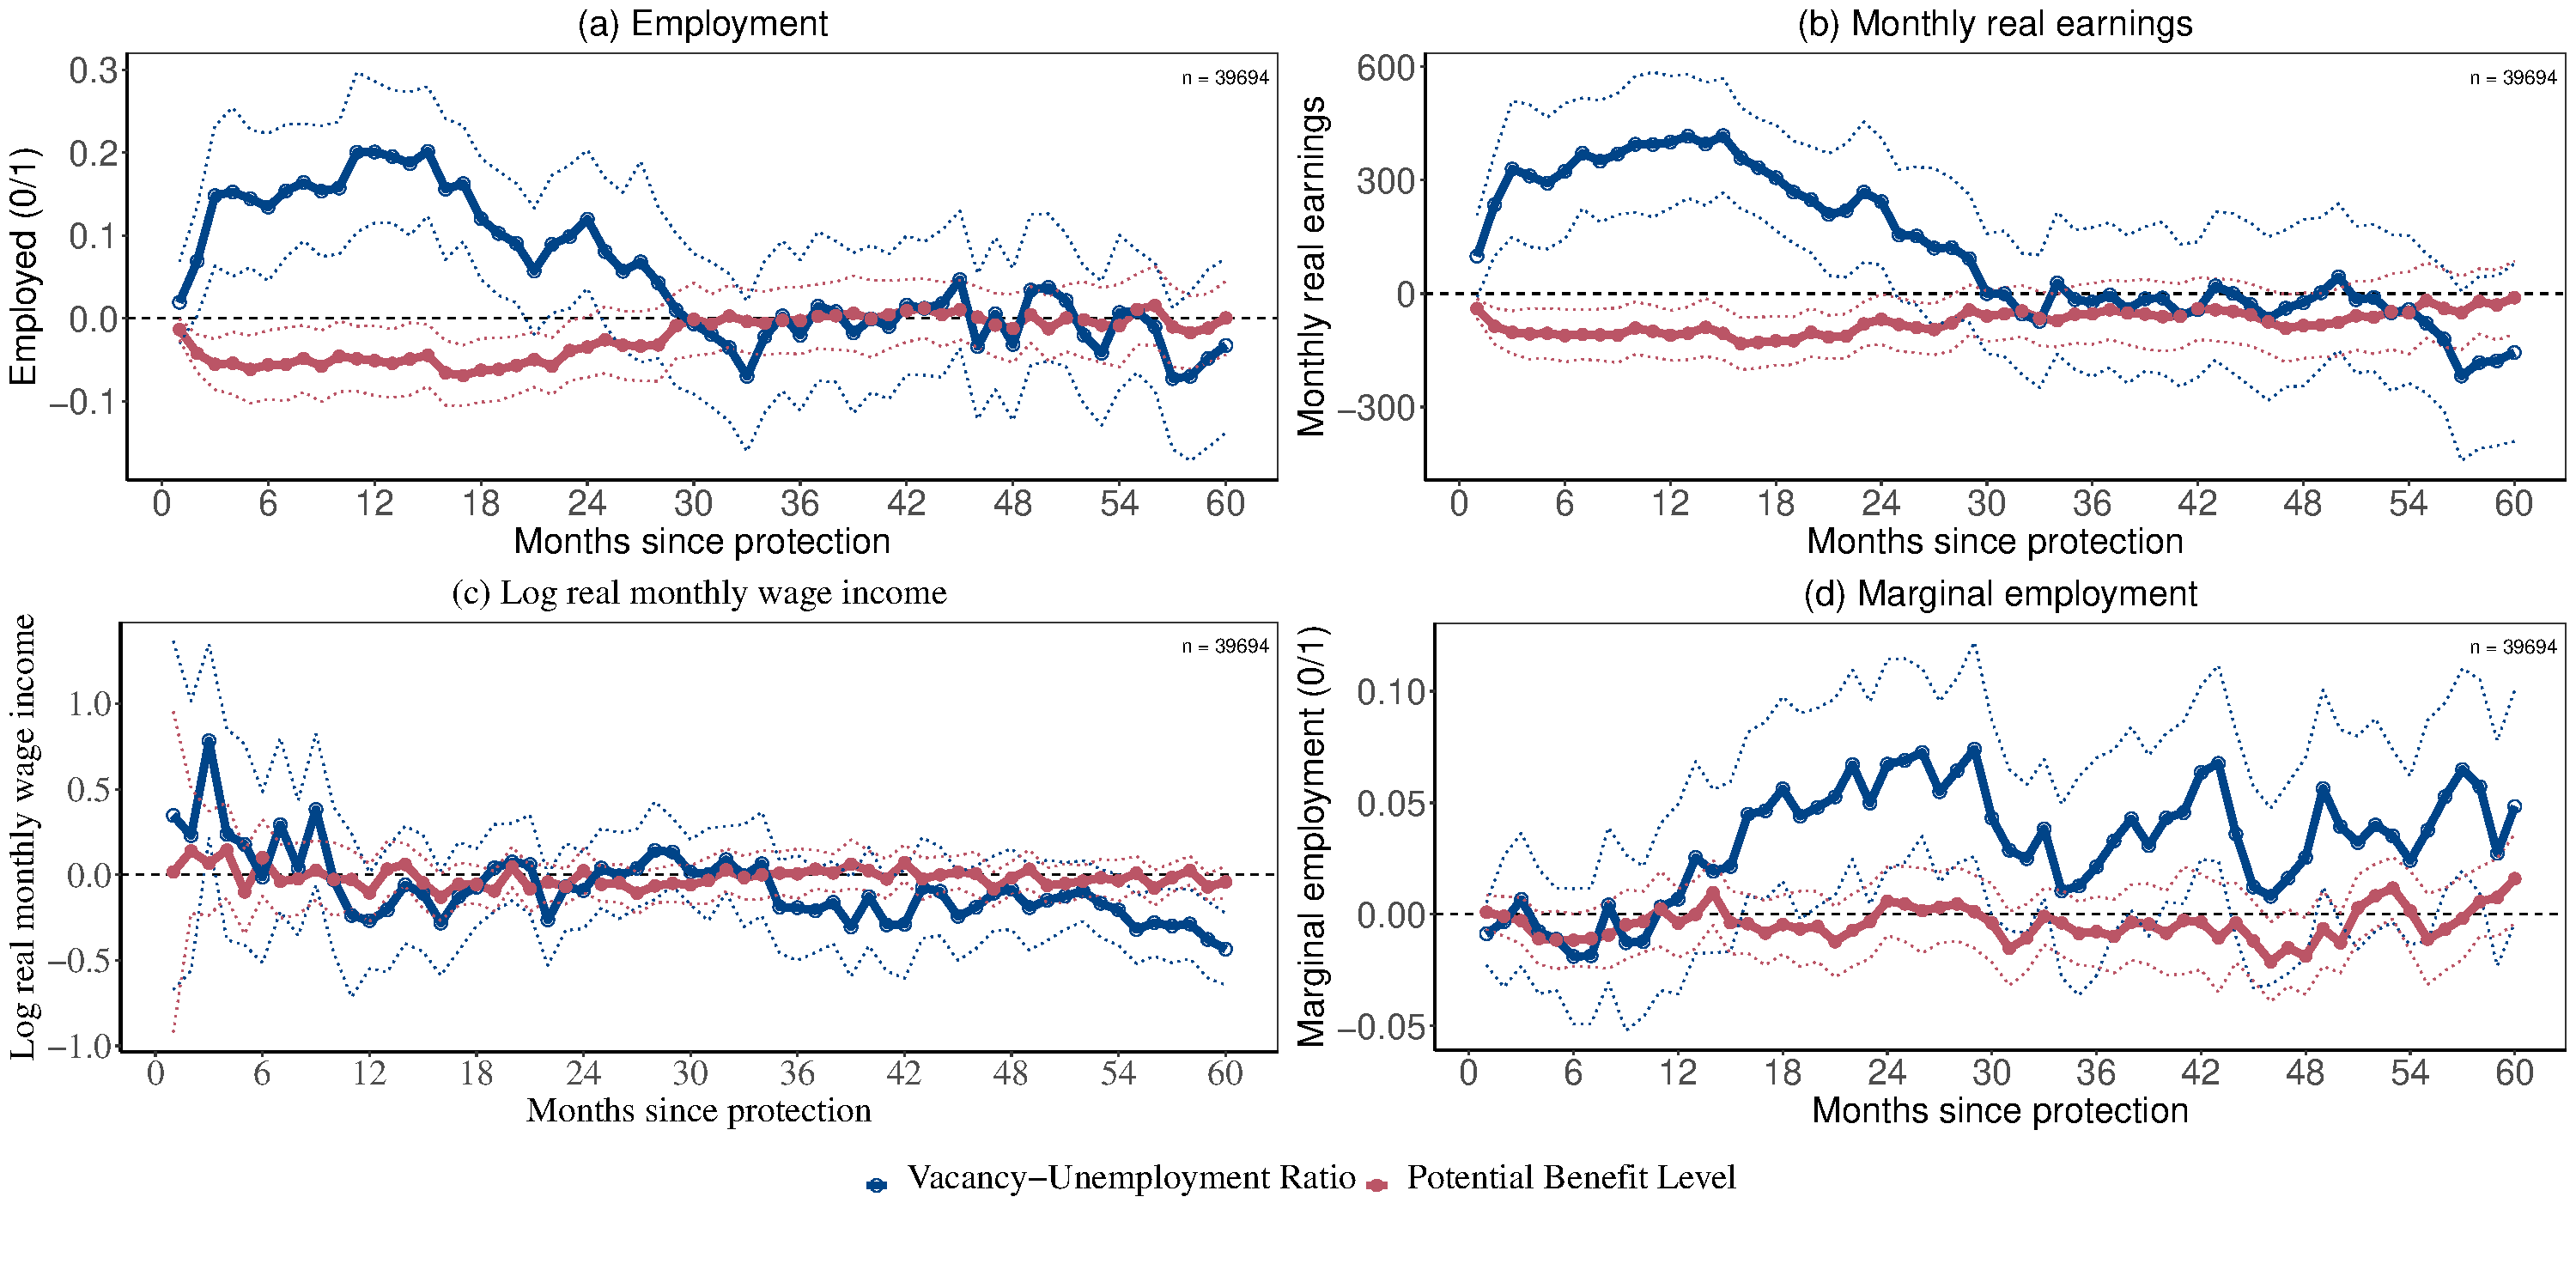
\includegraphics[scale=0.31]{figures/fig_employment_income.pdf}
    \end{center}
    \vspace{-0.5 cm}
    \fignote{\footnotesize \textit{Notes:} The x-axis shows the months since protection was received. The y-axis displays the effect of a one-unit increase in either i) the vacancy-to-unemployment ratio or ii) the potential benefit level, measured in €1,000 (real 2015 values), on selected outcomes. The panels show the effects on (a) having any type of part- or full-time employment (binary); panel (b) the unconditional monthly real earnings (in 2015 euro); panel (c) the log real monthly wage income (conditional on being employed); and panel (d) the probability of having a mini-job (below €406 in 2015). All regressions include a full set of arrival-group, year-month, and district-of-protection fixed effects. Additional control variables include age and age squared at immigration, gender, type of protection, family status at protection date, and country of origin. Standard errors are clustered at the state-year-of-protection level. Dashed lines indicate 95\% confidence intervals.}
\end{figure}

\FloatBarrier


\subsection{Effects on internal mobility}
 
Better labor market conditions and higher benefits should reduce the likelihood of relocating, which is very common among refugees after receiving protection (see Figure \ref{fig:descriptive_outcomes_main}). We show results for mobility in Figure~\ref{fig:mobility_results}. 

In Panel (a), we observe that an increase in the $IVUR$ has a statistically significant positive impact on the likelihood of refugees staying in the state. Specifically, a standard shift in the $IVUR$ leads to a 3.9 pp. increase in this probability in month twelve. Similarly, a standard shift in the $IPBL$ results in a 2.8 pp. increase in the same likelihood in month twelve. The effects become somewhat weaker over time but persist for 60 months, suggesting that enhanced welfare benefits and a strong labor market both positively influence the likelihood of refugees staying in their original state.

These findings are further supported by the observations in panel (b). Here, we note a consistent negative effect of the $IPBL$ on the likelihood of relocating to Vienna for those not initially assigned to Vienna. The $IVUR$  also has a negative but not persistent and only marginally significant effect.

The similarity of approaches allows for a direct comparison with the results of \citet{ferwerda2023}, who study the effect of current benefit levels on the probability of immigrants moving within Switzerland. They find that increasing benefits from less than 750 CHF to 751-1500 CHF increases the likelihood of staying by about 1.5 pp. while an increase to 1500-3000 CHF increases it by about 2 pp. Our effects are significantly larger, as a 2 pp. change in the probability is triggered by a roughly €200 change in benefit levels. A likely explanation is that the effects in the Austrian context are larger because the treatment is applied when refugees receive protection, when they are not yet strongly tied to a specific location and are potentially more mobile.\footnote{Alternatively, we can approximate an elasticity of the mover rate with respect to benefit levels. However, providing a single elasticity is difficult, as the result depends on the point of evaluation, i.e.\ which benefit level is 
considered (which varies substantially across states) and which mover rate is taken as the baseline. As an example, take Upper Austria.  The mean mover rate is 0.29. The reform reduced benefits from roughly €1,000 to €700 (incl. housing benefits), and we estimate that a €100 reduction increases the mover rate by roughly one pp. Evaluating the elasticity at the midpoint 
benefit level of €850 and an implied mover rate of 0.29, the percentage change in benefits is $-100/850 \approx -11.8\%$ while the corresponding change in the mover rate is $0.01/0.29 \approx 3.4\%$.
This yields an elasticity of $3.4/11.8 \approx 0.29$.}

\begin{figure}
    \caption{Effect of the $IVUR$ and $IPBL$ on mobility outcomes}
    \label{fig:mobility_results}
    \begin{center}
    \vspace{-0.5 cm}
    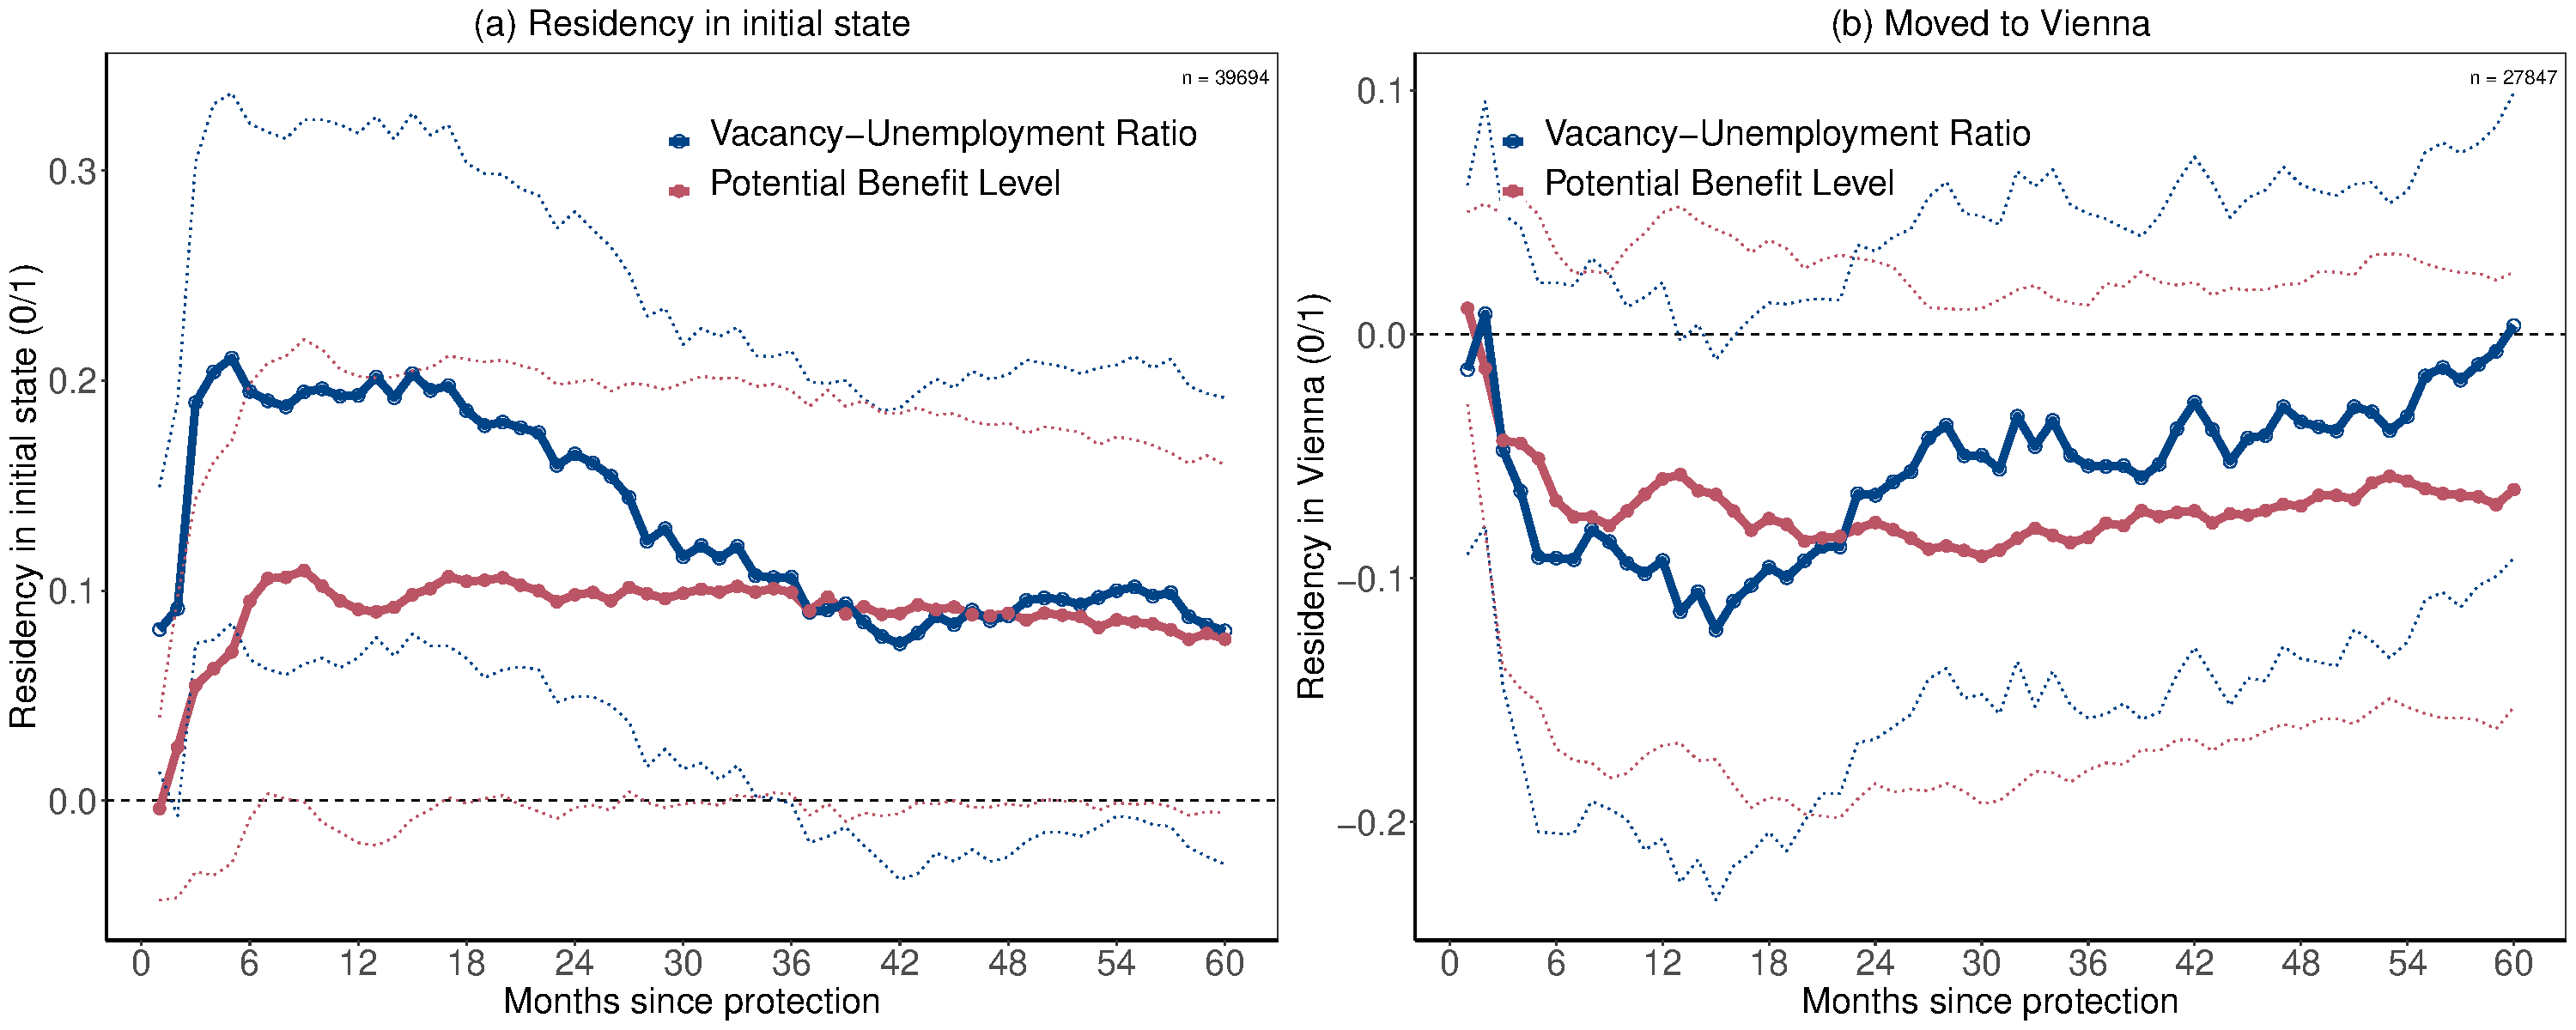
\includegraphics[scale=0.31]{figures/fig_mobility.pdf}
    \end{center}
    \fignote{\footnotesize \textit{Notes:} The x-axis shows the months since protection was received. The y-axis displays the effect of a one-unit increase in either i) the vacancy-to-unemployment ratio or ii) the potential benefit level, measured in €1,000 (real 2015 values), on selected outcomes. Panel (a) shows the effects on the probability of living in the state of protection; panel (b) shows the effect on moving to Vienna (conditional on residing outside Vienna at the time of protection). All regressions include a full set of arrival-group, year-month, and district-of-protection fixed effects. Additional control variables include age and age squared at immigration, gender, type of protection, family status at protection date, and country of origin. Standard errors are clustered at the state-year-of-protection level. Dashed lines indicate 95\% confidence intervals.}
\end{figure}

In Figure~\ref{fig:empl_reloc}, we show how the effects on employment and location choice interplay. A higher $IVUR$ positively affects the joint probability of being employed and in the initial state (panel (a)) and negatively affects the joint probability of being not employed and in another state (panel (d)). In other words, migrants stay because they are in employment instead of moving and needing to search for a job in another state. 

\begin{figure}
    \caption{Effect of the $IVUR$ and $IPBL$ on employment and location choice}
    \label{fig:empl_reloc}
    \begin{center}
    \vspace{-0.5 cm}
    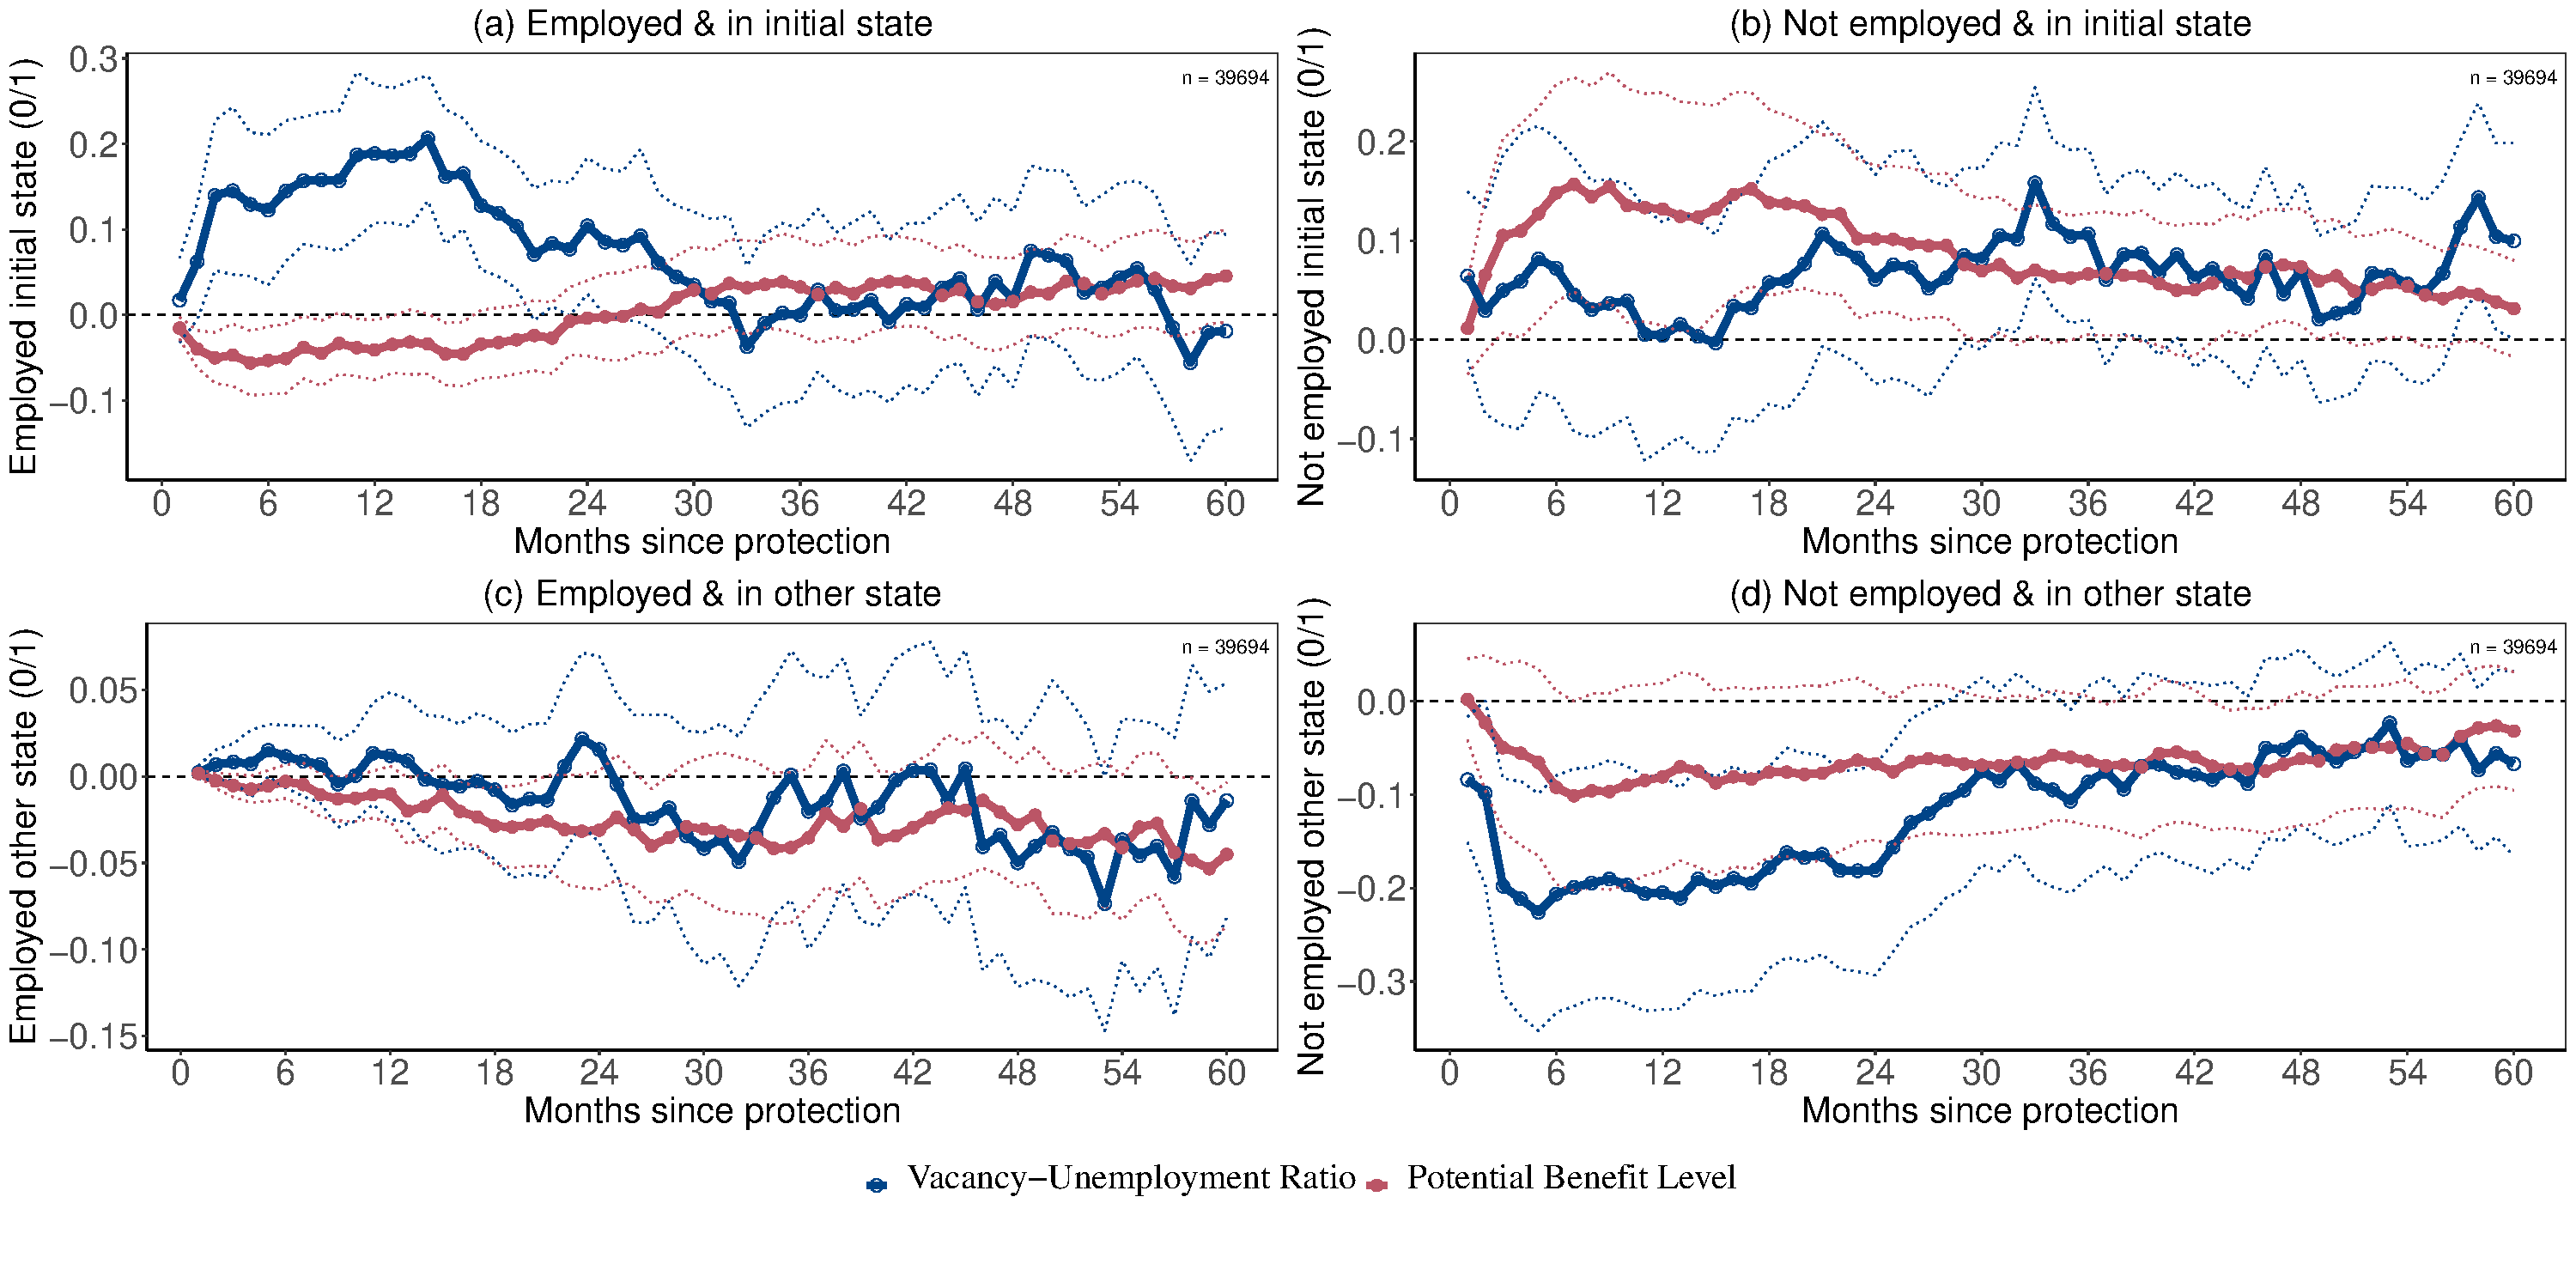
\includegraphics[scale=0.31]{figures/fig_employment_relocation.pdf}
    \end{center}
    \fignote{\footnotesize \textit{Notes:} The x-axis shows the months since protection was received. The y-axis displays the effect of a one-unit increase in either i) the vacancy-to-unemployment ratio or ii) the potential benefit level, measured in €1,000 (real 2015 values), on selected outcomes. Panel (a) shows the effects on the joint probability of being employed and living in the initial state; panel (b) shows the effect on the joint probability of being not employed and living in the initial state. Panel (c) shows the effects on the joint probability of being employed and living in another state; panel (d) shows the effect on the joint probability of not being employed and living in another state. All regressions include a full set of arrival-group, year-month, and district-of-protection fixed effects. Additional control variables include age and age squared at immigration, gender, type of protection, family status at protection date, and country of origin. Standard errors are clustered at the state-year-of-protection level. Dashed lines indicate 95\% confidence intervals.}
\end{figure}

In contrast, the $IPBL$ has a stronger effect on the joint probability of being not employed and in the initial state (panel (b)). However, this is primarily due to a higher likelihood of remaining in the state, rather than to changing employment prospects. This becomes apparent from the negative effect on not being employed and in another state (panel (d)).

This suggests that strong labor markets increase the probability that individuals remain in their initial state, owing to job availability. In contrast, weak labor markets might incentivize relocation to another state without prospects of work in the destination state. Additionally, these findings indicate that benefit levels are relevant for the location choice but less so for employment trajectories.

\FloatBarrier

\subsection{Effects on receiving social support}

The third group of outcomes consists of measures of social support receipt. Figure~\ref{fig:welfare_results} shows the effects on the likelihood of (a) utilizing services from the public employment service and (b) receiving welfare benefits.

We do not observe any effect of the $IVUR$ or $IPBL$ on utilizing PES services (Panel (a)). If anything, a higher $IPBL$ has a small negative effect in the first nine months.

%Nevertheless, the zero average effect might mask two cont Individuals who do not receive support might either have secured regular employment, negating the need for further support services, or might be lacking such services due to underperformance. These contrasting scenarios could neutralize each other, resulting in the observed insignificance.

Panel (b) shows a significant negative impact of the $IVUR$ on the probability of receiving welfare benefits in the first 30 months. Interestingly, the magnitude of this effect is consistent with the positive effect of the $IVUR$ on employment (Figure \ref{fig:economic_results}, Panel (a)). Furthermore, the impact on receiving welfare benefits diminishes and becomes statistically insignificant after 30 months, mirroring the trajectory of the employment effect. This suggests that refugees who secure employment due to favorable local labor market conditions are less likely to rely on welfare benefits.

Similarly, we observe that a higher $IPBL$ has a small but significant effect on the likelihood of receiving welfare benefits, particularly in the years 2 and 3 after receiving protection. The effect is largest about 24 months after receiving protection, when a standard shift in $IPBL$ increases the probability of receiving welfare benefits by about 2.5 pp. Again, the pattern mirrors the effect of $IPBL$ on employment.

%A shift in the $IVUR$ from the first to the third quartile reduces the likelihood of receiving welfare benefits by 4.9 percentage points, relative to a base rate of 76.1\% of refugees obtaining welfare benefits in month 12.

\begin{figure}
    \caption{Effect of the $IVUR$ and $IPBL$ on selected social support outcomes}
    \label{fig:welfare_results}
    \begin{center}
    \vspace{-0.5 cm}
    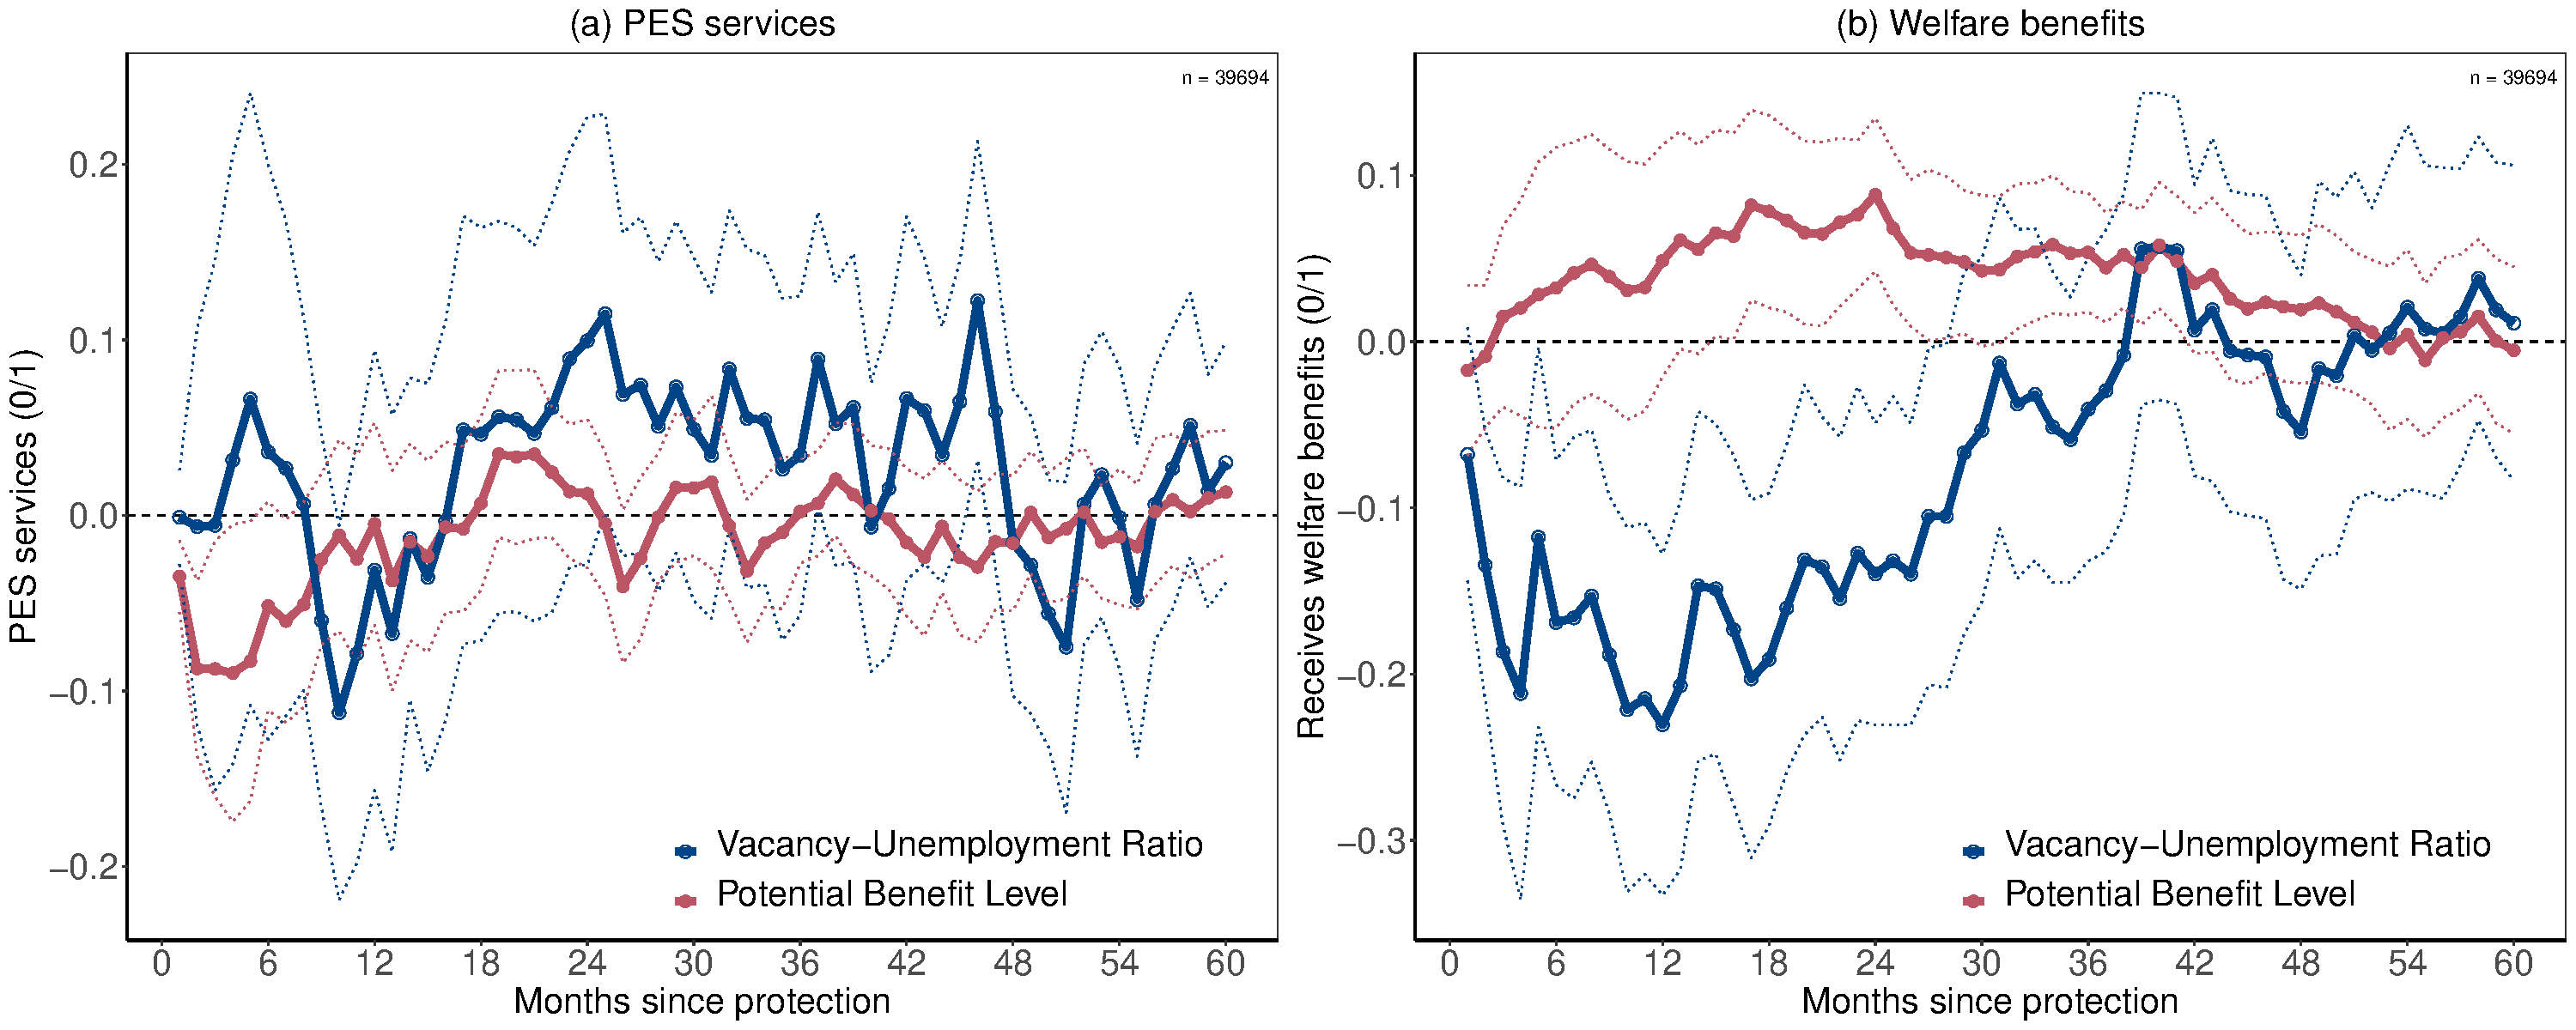
\includegraphics[scale=0.31]{figures/fig_social_support.pdf}
    \end{center}
    \fignote{\footnotesize \textit{Notes:} The x-axis shows the months since protection was received. The y-axis displays the effect of a one-unit increase in either i) the vacancy-to-unemployment ratio or ii) the potential benefit level, measured in €1,000 (real 2015 values), on selected outcomes. The panels show the effects on (a) the probability of making use of PES services and (b) the probability of receiving welfare benefits. All regressions include a full set of fixed effects for arrival group, year-month, and district of protection. Additional control variables include age and age squared at immigration, gender, type of protection, family status at protection date, and country of origin. Standard errors are clustered at the state-year-of-protection level. Dashed lines indicate 95\% confidence intervals.}
\end{figure}

\FloatBarrier




\subsection{Interplay of labor market tightness and benefit levels}

Our main specification, as presented in Equation \ref{eq:main}, estimates how $IVUR$ and $IPBL$ independently affect refugees' economic and social integration after receiving protection. To further explore the relationships between these variables, we introduce an interaction term between $IVUR$ and $IPBL$ in Equation \ref{eq:main_interaction}:

A negative cross-partial of $IVUR$ and $IPBL$ on employment is consistent with a standard equilibrium search framework \citep{pissarides2000}, in which higher labor market tightness raises the offer arrival rate, so the disincentive effect of a higher reservation wage from more generous benefits binds more tightly when offers are plentiful. \citet{schmieder2016} document the same cross-partial empirically for unemployment insurance across varying labor market conditions.

\begin{equation}\label{eq:main_interaction}
\begin{aligned}
Y_{i,t} = & \, \alpha_t + \beta_{1,t} IVUR_{d_0,t_0} + \beta_{2,t} IPBL_{f,p,s_0,t_0} + \beta_{3,t} IVUR_{d_0,t_0} \times IPBL_{f,p,s_0,t_0} \\
& + \gamma_{t_0} + \delta_{g} + \eta_{d_0} + X_{i}\Delta_t + \epsilon_{i,t},
\end{aligned}
\end{equation}

This specification allows us to calculate and interpret the effects of changes in the $IPBL$ for different levels of labor market tightness.

Table \ref{tab:interactions} reports the results for selected outcomes twelve months after receiving protection. For ease of interpretation, we demeaned $IVUR$ and $IPBL$. The coefficients for the main effects remain comparable to our previous results in direction, magnitude, and statistical significance. The interaction term has a significant, opposing effect on the probability of being in employment and receiving welfare benefits (columns (1) and (4), respectively). For the probability of remaining in the initial state in column (2), we find no statistically significant effect of the interaction, but we find a positive and significant effect on the probability of receiving assistance by the PES in column (3).

The marginal effects are calculated for the $IPBL$. Therefore, we fix the $IVUR$ at zero on the first row, the mean in the second row and at 0.2 above the mean in the third row.

Column (1) shows the effect of changes in benefit levels on the probability of being employed at different levels of labor market tightness. As predicted by the search framework above, changes in benefit levels have practically no effect on the employment probability when the labor market is slack. However, benefit levels affect employment probability strongly when the labor market is tight. We see the inverse effects for the receipt of welfare benefits (column (4)).
These results are in line with both the search prediction and the empirical findings of \citet{dustmann2024}, who find that cuts in welfare benefits in Denmark only affect the employment probability in strong labor markets.

Column (3) suggests that when the labor market is tight, increasing benefits increases the likelihood of receiving assistance from the PES. This is potentially due to the combination of the incentives for public agencies to fill the labor demand, but also to reduce the fiscal cost due to high benefit levels.

\begin{table}
	\caption{Effects of $IVUR$ and $IPBL$ with interactions of treatment variables and marginal effects of $IPBL$ for different levels of $IVUR$, twelve months after protection}
	\label{tab:interactions}
	\begin{threeparttable}
		\begin{small}
			\begin{tabular}{lcccc}				\centering
\begin{tabular}{lcccc}
\hline
& (1) & (2) & (3) & (4) \\
& In employment & In initial state & PES support & Welfare benefits \\ 
\hline
\textbf{Coefficients} \\
IVUR & 0.188*** & 0.189** & -0.021 & -0.218*** \\
& (0.044) & (0.062) & (0.056) & (0.048) \\ 
IPBL & -0.050** & 0.091** & -0.005 & 0.048* \\
& (0.018) & (0.030) & (0.025) & (0.024) \\ 
IVUR:IPBL & -0.294*** & -0.091 & 0.230*** & 0.280*** \\
& (0.043) & (0.112) & (0.055) & (0.071) \\ 
\hline
\textbf{Marginal Effects} \\
IPBL (IVUR=0) & 0.006 & 0.108 & -0.049 & -0.006 \\
IPBL (IVUR=0.192) & -0.050 & 0.091 & -0.005 & 0.048 \\
IPBL (IVUR=0.392) & -0.109 & 0.073 & 0.041 & 0.104 \\
\hline
\end{tabular}
			\end{tabular}
		\end{small}
		\begin{tablenotes} 
			\begin{footnotesize}
				\begin{spacing}{1}
					\textit{Notes:} The upper part of the table reports OLS estimates for $IVUR$, $IPBL$ and their interaction. The lower part reports marginal effects for $IPBL$, fixing $IVUR$ at zero, the mean (0.192) or 0.2 above the mean. The column title shows the outcome variable. All regressions include a full set of arrival-group, year-month, and district-of-protection fixed effects. Additional control variables include age and age squared at immigration, gender, type of protection, family status at protection date, and country of origin. Standard errors are clustered at the state-year-of-protection level. */**/*** denote statistical significance at the 10/5/1 percent level.
				\end{spacing}
			\end{footnotesize}
		\end{tablenotes}
	\end{threeparttable}
\end{table}


\FloatBarrier

\subsection{Effect heterogeneity by gender}

One notable observation is the significant disparity in labor market integration between genders, with women's employment rates at only 20\% even five years post-protection, in stark contrast to men's, which is 60\% (see Figure \ref{fig:descriptive_outcomes_main}).

In this section, we investigate whether men and women also differ in their reactions to $IVUR$ and $IPBL$.  For this, we conduct the analysis separately for men and women with the results shown in Figure \ref{fig:gender}. 

\begin{figure}
    \caption{Effect heterogeneity by gender}
    \label{fig:gender}
    \begin{center}
    \vspace{-0.5 cm}
    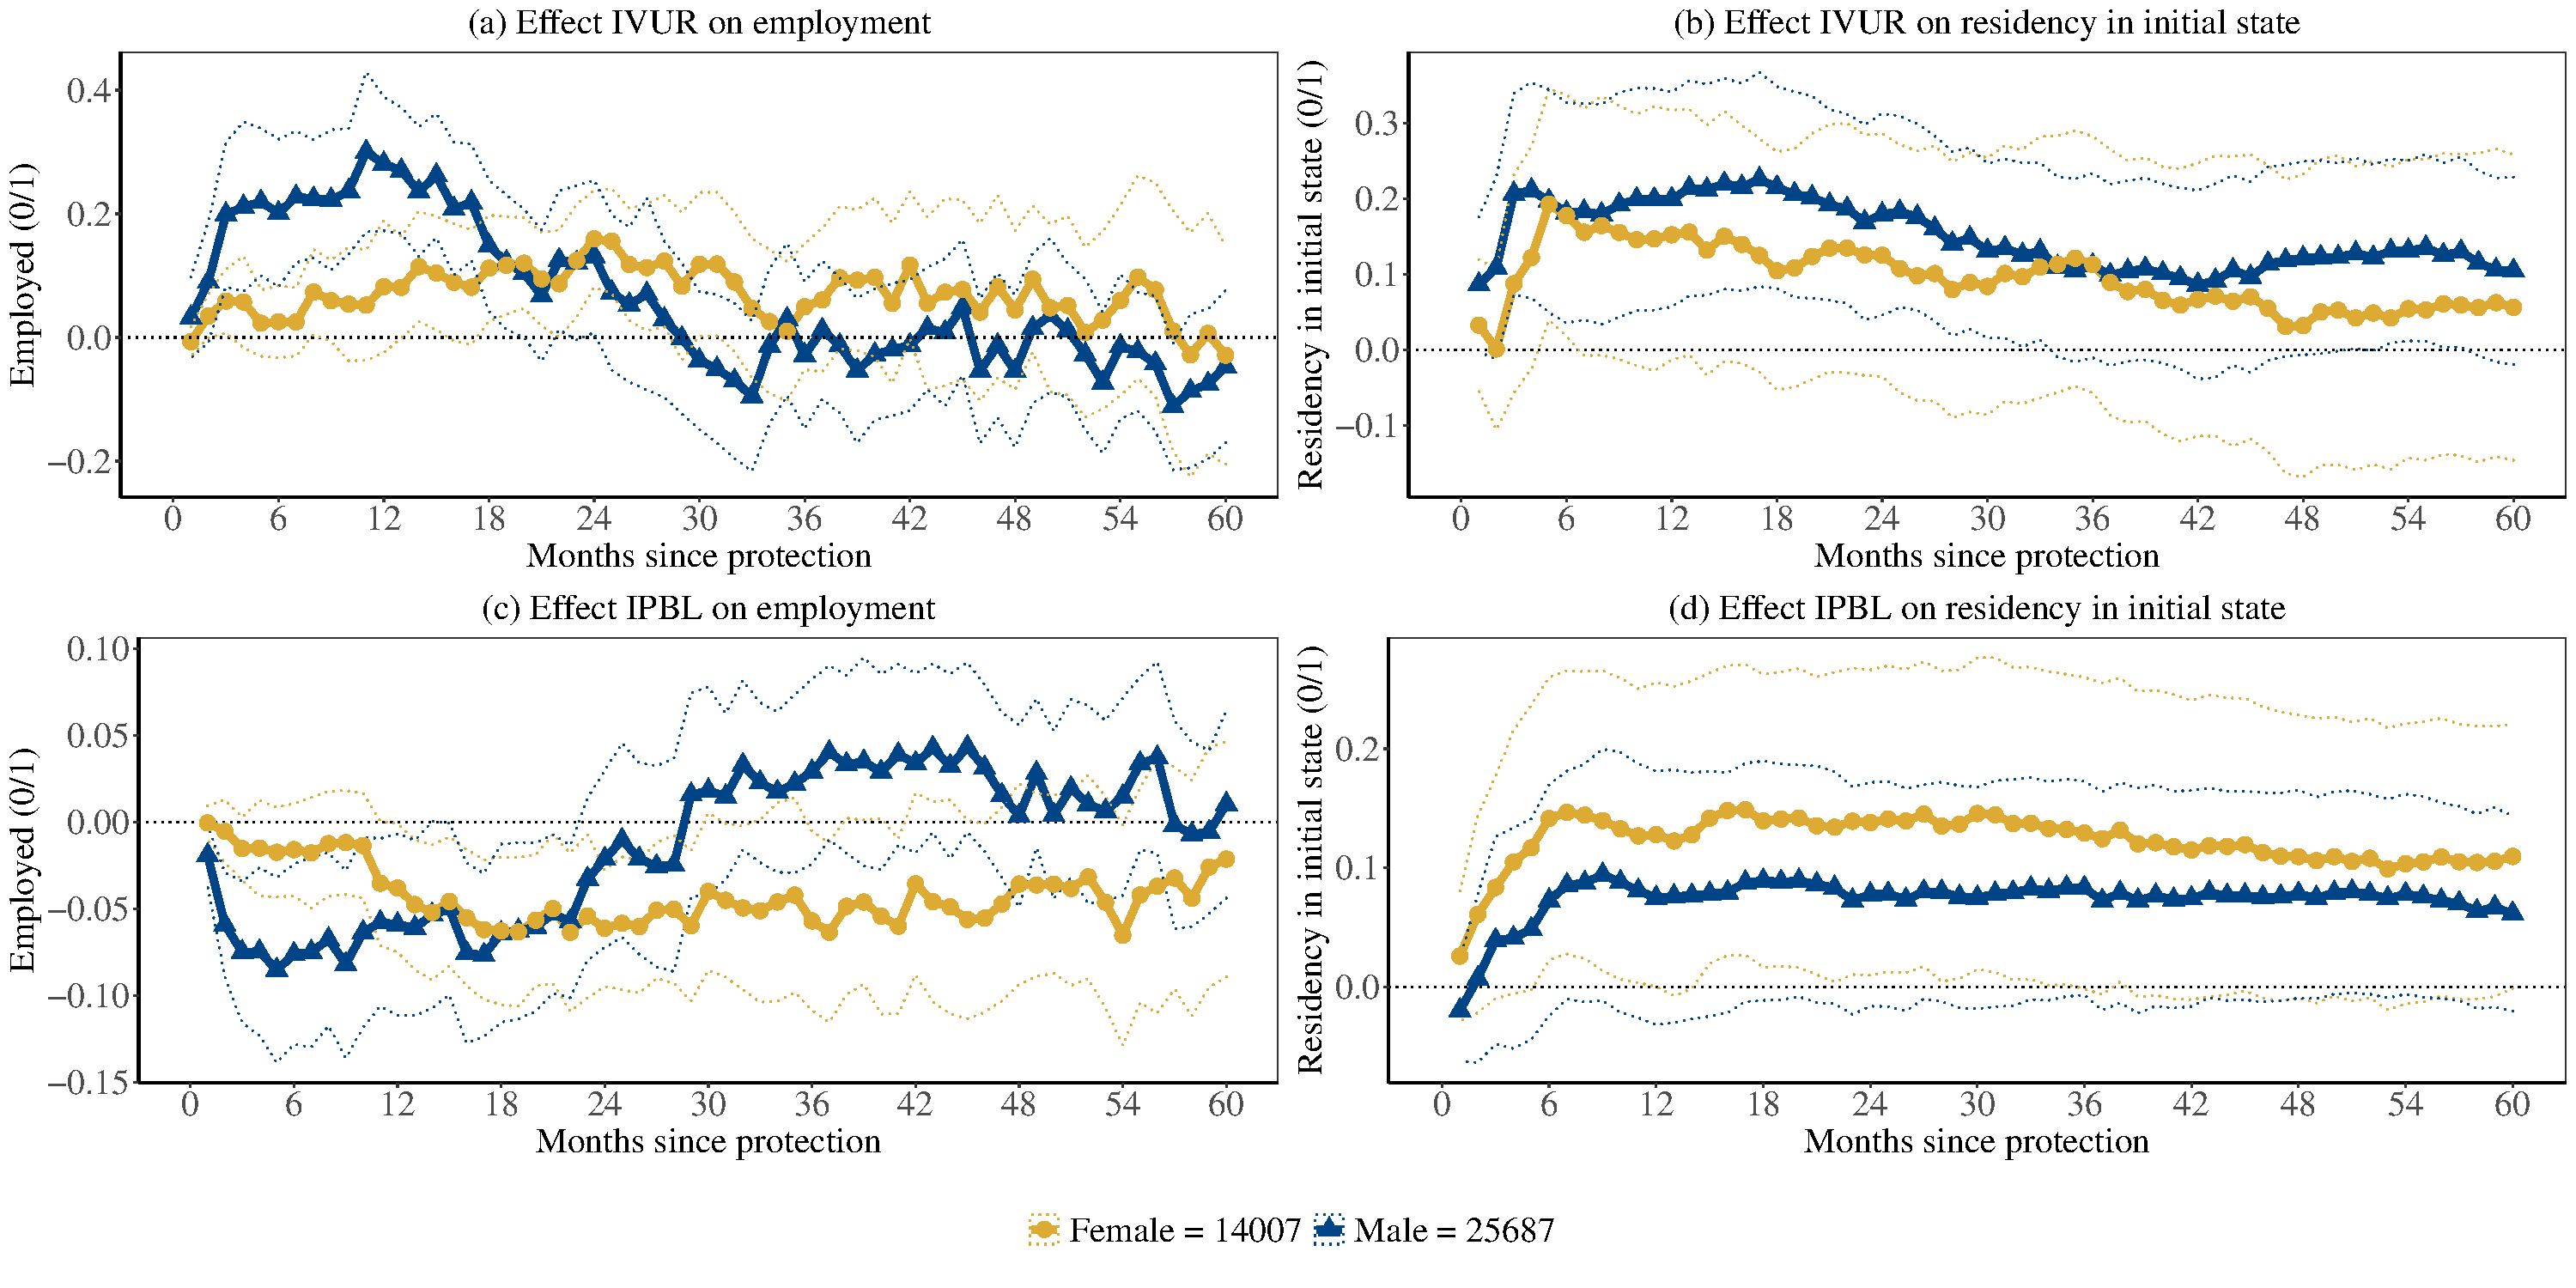
\includegraphics[scale=0.31]{figures/fig_gender.pdf}
    \end{center}
    \vspace{-0.5em}
\fignote{\footnotesize \textit{Notes:} The x-axis shows the months since protection was received. The y-axis displays the effect of a one-unit increase in either (i) the vacancy-to-unemployment ratio or (ii) the potential benefit level, measured in €1,000 (real 2015 values), on selected outcomes. Panels (a) and (b) show the effects of $IVUR$ on employment and on the probability of staying in the initial state, respectively. Panels (c) and (d) show the effects of $IPBL$ on employment and on the probability of staying in the initial state, respectively. Estimates are shown separately for men and women. All regressions include a full set of arrival-group, year-month, and district-of-protection fixed effects. Additional control variables include age and age squared at immigration, type of protection, family status at protection date, and country of origin. Standard errors are clustered at the state-year-of-protection level. Dashed lines indicate 95\% confidence intervals.}
\end{figure}

Panel (a) shows the effects of $IVUR$ on employment. $IVUR$ strongly affects the employment probability of men in the first 18 months after protection, but has hardly any effect on women. Still, for women, we do see some positive effects from around month twelve onwards. While this effect is small in absolute terms, it is not in relative terms, given the extremely low employment rate of female refugees. Panel (b) shows the effect of $IVUR$ on mobility. Point estimates are slightly larger for men, but overall, the pattern is similar. Panel (c) shows the effect of $IPBL$ on employment. While men initially reduce their employment more in response to higher benefits, the effect persists only for 30 months. For women, the negative effect of $IPBL$ on employment is small but relatively persistent. Finally, Panel (d) shows that the effect of $IPBL$ on the likelihood of staying in the state is somewhat stronger for women and persistent for both groups. 

These findings align with the behavior predicted by traditional household models. When men primarily engage in market activities and actively seek employment, their sensitivity to labor market tightness is expected to be higher. For women, labor market tightness is less influential. Regarding mobility, labor market tightness indirectly affects the non-working partner's decisions, especially if the household relocates due to the male partner's unfavorable labor market conditions. Conversely, as men's attachment to the labor market strengthens over time, the significance of benefit levels wanes. However, benefits continue to play a crucial role for women, significantly influencing location choices within Austria.


\subsection{Relevant initial labor market}
As noted by \citet{aslund_when_2007}, it is not clear at what point in time initial local labor market conditions should be measured for refugees. While most of the literature focuses on labor market conditions at the time of immigration, institutional factors limit refugees' labor market access until they have been granted protection (12 months after arrival in our sample). 

Hence, to compare our results to the standard specification in the literature, we add $IVUR$ and $IPBL$ measured at the time of immigration to our regressions. Table \ref{tab:ivuripbl_arrival} shows the results for two outcomes, employment and residency in the initial state, for month 12 after receiving protection.

\begin{table}
  \centering
  \caption{Effects of IVUR and IPBL at Approval on Employment and Residency \\* controlling for IVUR and IPBL at Arrival}
  \label{tab:ivuripbl_arrival}
  \begin{talltblr}[         %% tabularray outer open
entry=none,label=none,
note{}={},
]                     %% tabularray outer close
{                     %% tabularray inner open
colspec={Q[]Q[]Q[]},
column{1}={halign=l,},
column{2}={halign=c,},
column{3}={halign=c,},
}                     %% tabularray inner close
\toprule
& Employed & Residency in initial state \\ \midrule %% TinyTableHeader
IVUR at approval & \num{0.195}*** & \num{0.183}** \\
& (\num{0.050})  & (\num{0.061}) \\
IVUR at arrival  & \num{-0.010}   & \num{0.009}   \\
& (\num{0.059})  & (\num{0.061}) \\
IPBL at approval & \num{-0.017}   & \num{0.183}*  \\
& (\num{0.028})  & (\num{0.077}) \\
IPBL at arrival  & \num{-0.050}   & \num{-0.138}  \\
& (\num{0.026})  & (\num{0.073}) \\
\bottomrule
\end{talltblr}

    \\
  		\begin{tablenotes} 
			\begin{footnotesize}
				\begin{spacing}{1}
					\textit{Notes:} The table reports coefficients from OLS regressions estimating the effects at month 12 after receiving protection of i) the vacancy-to-unemployment ratio (IVUR) and ii) the potential benefit level (IPBL) measured in €1,000 (real 2015 values), both at the time of approval and arrival, on two outcomes: employment status (left) and residency in the initial state (right). All regressions include a full set of arrival-group, year-month, and district-of-protection fixed effects, as well as additional controls for age and age squared at immigration, gender, type of protection, family status at protection date, and country of origin. Standard errors are clustered at the state-year-of-protection level. */**/*** denote statistical significance at the 10/5/1 percent level.
				\end{spacing}
			\end{footnotesize}
		\end{tablenotes}
\end{table}

Controlling for $IVUR$ and $IPBL$ at arrival leaves the effects of $IVUR$ at approval on employment and residency virtually unchanged. For $IPBL$ at approval, the point estimate on employment is roughly halved and loses statistical significance, while the effect on residency approximately doubles. 

In contrast, both $IVUR$ and $IPBL$ at arrival are not statistically significant for either outcome. 
\FloatBarrier
\subsection{Mechanisms}\label{sec:mech}
%\footnote{The analysis in this section is preliminary and the measure for desired occupations is currently refined.}
In this section we explore whether a particular type of occupations drive the $IVUR$ results. For this, we generate alternative measures of the $IVUR$. First, by desired occupations, which are usually registered by the caseworkers at the PES for each job-seeker. And second, by seasonal and non-seasonal jobs.
Additionally, we explore the concern, that the benefit cuts could be politically driven by controlling for the vote share intentions for the FPÖ (Freedom Party of Austria), a right-wing populist party.

\vspace{0.5cm}
\noindent\textbf{Labor demand by most desired occupations.}\hspace{0.5cm} A broad measure of labor demand reflects the overall situation of the local labor market. However, many jobs that firms are seeking to fill might not be accessible to refugees with short tenures in the host country due to a lack of necessary language skills or recognized qualifications. To investigate whether the occupations in demand matter, we use the detailed nature of the vacancy data to create alternative versions of the $IVUR$.

First, we create a measure of demand for occupations with particularly low entry barriers. The PES records \textit{desired occupations} for every person registering with the PES. Desired occupations are not necessarily the jobs a job seeker desires, but those that a caseworker considers realistic based on the job seeker’s prior experience and skills. We see a strong clustering for refugees, with four occupations accounting for more than 50\% of the desired occupations: construction, cleaning, cooking and kitchen assistance, and general manual labor. Thus, we consider labor demand in these four occupations.

Figure \ref{fig:occ_ivur} shows the effect of the $IVURs$ in desired occupations on employment and mobility. The impact of labor demand in desired occupations on employment is approximately three times larger than that of the overall measure (left figure). However, this effect is short-lived, diminishing sharply after 18 months. In contrast, mobility is also strongly affected in the short term, and the effects, while somewhat declining, persist over the 60-month observation period (right figure).\footnote{This analysis has two caveats. First, these jobs account for only a small fraction of all vacancies, and the regional variation in this $IVUR$ measure is significantly smaller. Thus, while the effect of labor demand in this occupation is large, the low variation implies that the overall effect of demand in these occupations on explaining mobility and employment differences between regions is small. Second, labor demand in these occupations might be correlated with labor demand in other occupations. In this case, the estimates would be upward-biased. To address this concern, we run a model that includes labor demand in all other but the desired occupations.
The estimated effect of demand in the other occupations is slightly smaller but similar to the main result. Desired occupations have a stronger but more short-lived effect on employment than other occupations. However, they account for only a small share of all occupations.
 % (not included in this version). 
}%, while the effect of $IPBL$ on employment is -0.051367, and on residing in the initial state is 0.09056.} 

\begin{figure}
    \caption{Effect of $IVUR$ in desired occupations on employment and mobility}
    \label{fig:occ_ivur}
    \begin{center}
    \vspace{-0.5 cm}
    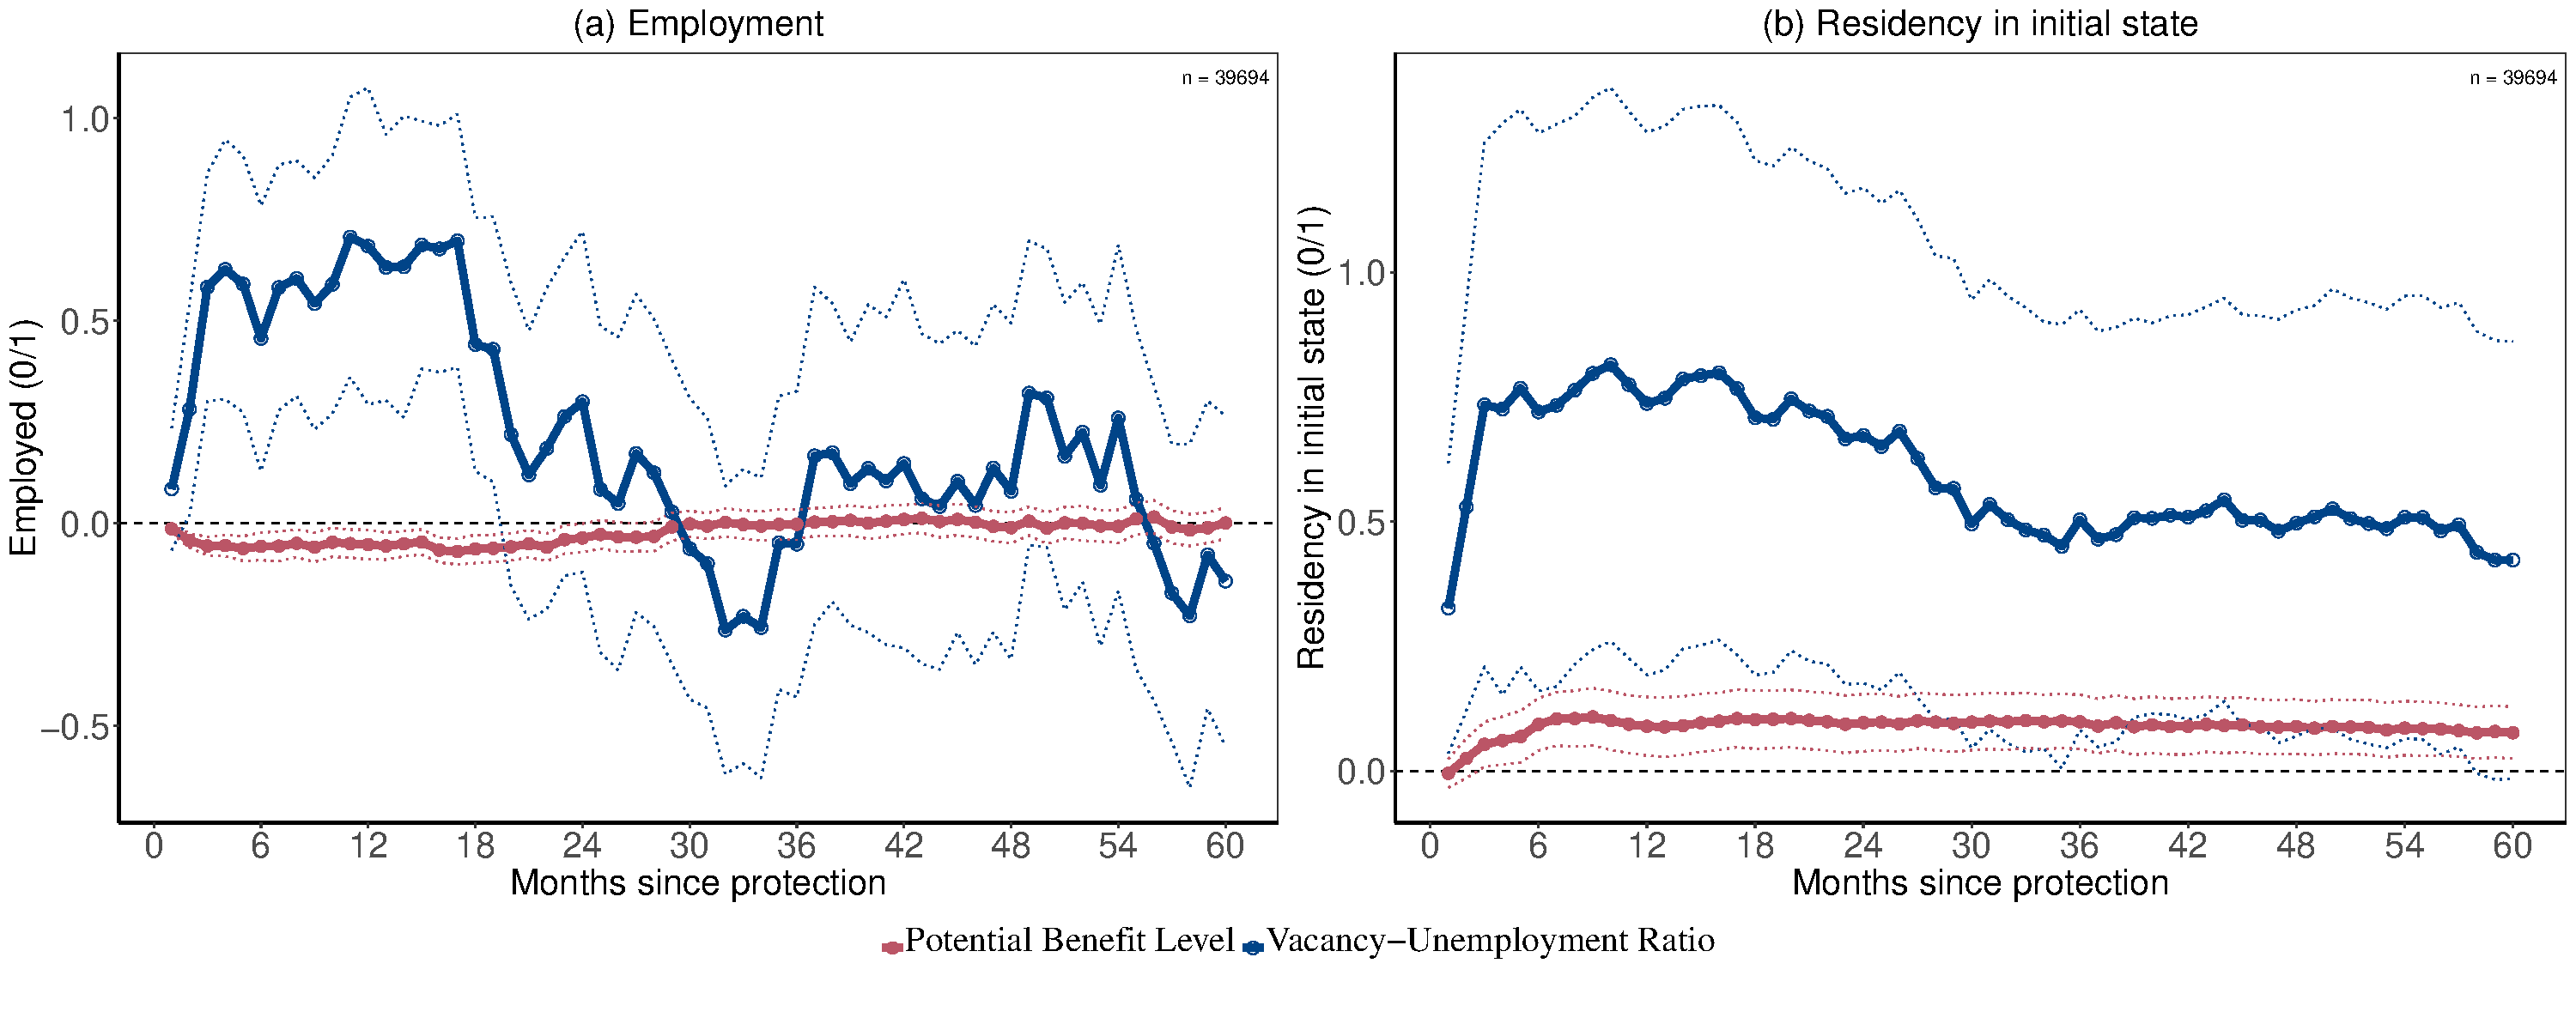
\includegraphics[scale=0.31]{figures/rob/fig_rob_labor_mobility_most_desired.pdf}
    \end{center}
    \vspace{-0.5cm}
    \fignote{\footnotesize \textit{Notes:} The x-axis shows the months since protection was received. The y-axis displays the effect of a one-unit increase in either i) the occupation-specific vacancy-to-unemployment ratio or ii) the potential benefit level, measured in €1,000 (real 2015 values), on employment (left) and mobility (right). All regressions include a full set of arrival-group, year-month, and district-of-protection fixed effects. Additional control variables include age and age squared at immigration, gender, type of protection, family status at protection date, and country of origin. Standard errors are clustered at the state-year-of-protection level.}
\end{figure}


\vspace{0.5cm}
\noindent\textbf{Labor demand by seasonal occupations.}\hspace{0.5cm} We create a measure for demand in jobs labeled as seasonal occupations, often found in the tourism industry. These jobs are of particular interest as they reflect truly short-term opportunities rather than long-term economic perspectives.

For both types of occupations, we create measures for the $IVUR$ by dividing the number of open positions in the respective categories by the number of job seekers. Note that we do not restrict job seekers to those looking in these specific occupations, as they often search in a broader range of fields.

\begin{figure}
    \caption{Effect of $IVUR$ in seasonal occupations on employment and mobility}
    \label{fig:seasonal_ivur}
    \begin{center}
    \vspace{-0.5 cm}
    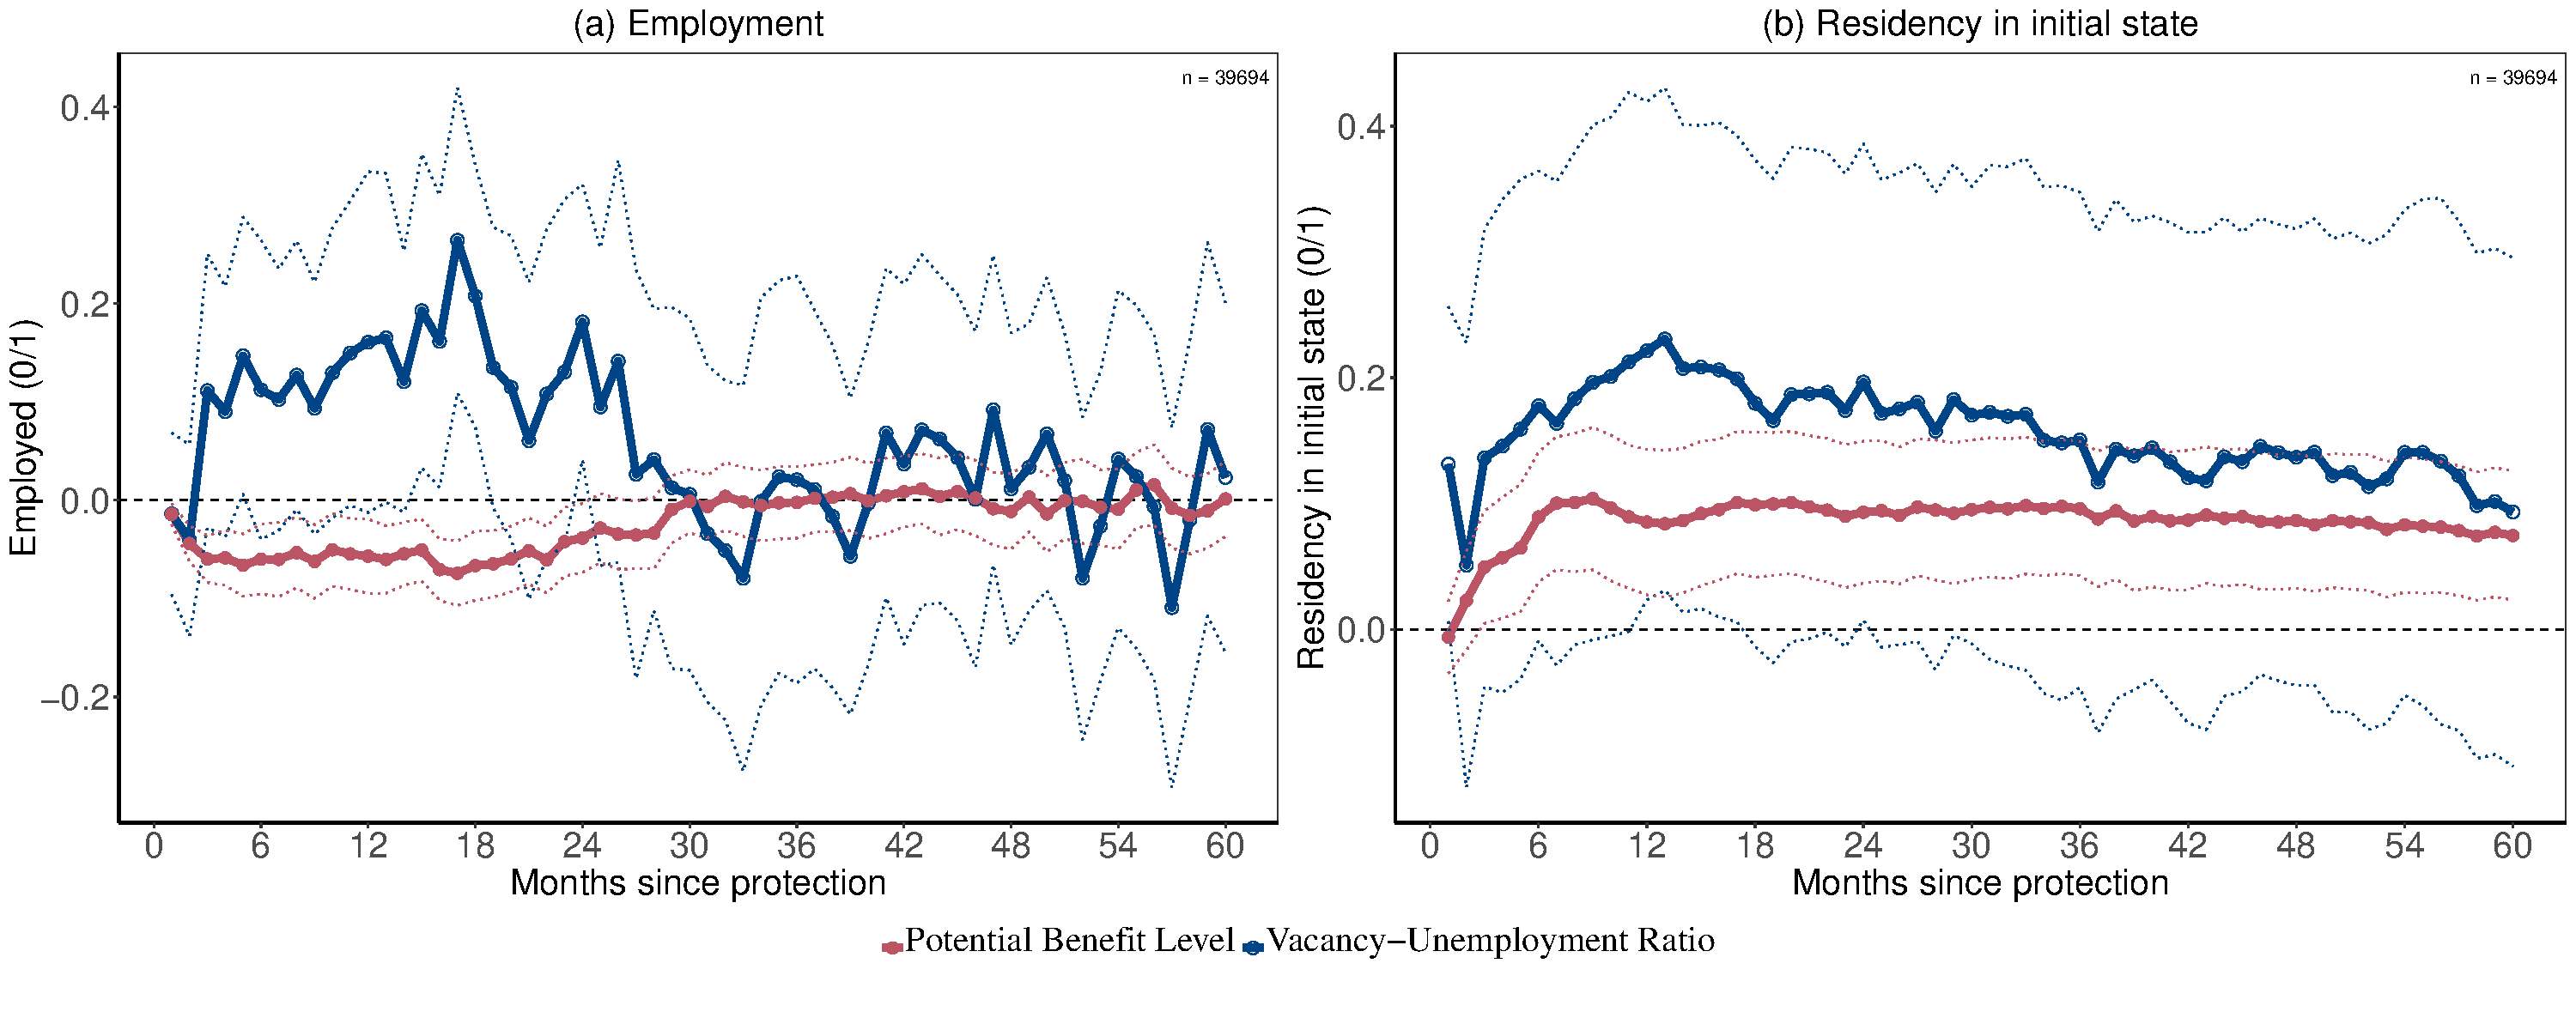
\includegraphics[scale=0.31]{figures/rob/fig_rob_labor_mobility_seasonal.pdf}
    \end{center}
    \fignote{\footnotesize \textit{Notes:} The x-axis shows the months since protection was received. The y-axis displays the effect of a one-unit increase in either i) the occupation-specific vacancy-to-unemployment ratio or ii) the potential benefit level, measured in €1,000 (real 2015 values), on employment (left) and mobility (right). All regressions include a full set of arrival-group, year-month, and district-of-protection fixed effects. Additional control variables include age and age squared at immigration, gender, type of protection, family status at protection date, and country of origin. Standard errors are clustered at the state-year-of-protection level.}
\end{figure}

Figure \ref{fig:seasonal_ivur} shows the effects of labor demand in seasonal occupations, Figure \ref{fig:non_seasonal_ivur} for the non-seasonal occupations. It is important to note that due to district-fixed effects, this demand does not reflect differences in the regional economic structure, such as tourist areas. Instead, it reflects pure short-term demand for labor due to likely idiosyncratic reasons. For example, certain weather conditions might increase or decrease labor demand in the tourist industry or agriculture at specific times \citep{baumgartner2023}. The demand for these seasonal occupations should thus not influence forward-looking decisions based on expected labor market chances. Nevertheless, we find that seasonal labor demand increases the likelihood of employment and persistently increases the likelihood of staying, with the effects being only slightly smaller than for non-seasonal occupations. 

Together, these results indicate that refugees' decisions are driven by immediate constraints rather than long-term considerations. The immediate opportunities provided by these jobs facilitate the difficult transition from refugee shelters to independent housing. Once refugees have transitioned, they are more likely to remain in their original location. However, these initial job opportunities do not set refugees on a different career track with long-term implications.

\begin{figure}
    \caption{Effect of the $IVUR$ for non-seasonal occupations and $IPBL$ on employment and location choice}
    \label{fig:non_seasonal_ivur}
    \begin{center}
    \vspace{-0.5 cm}
    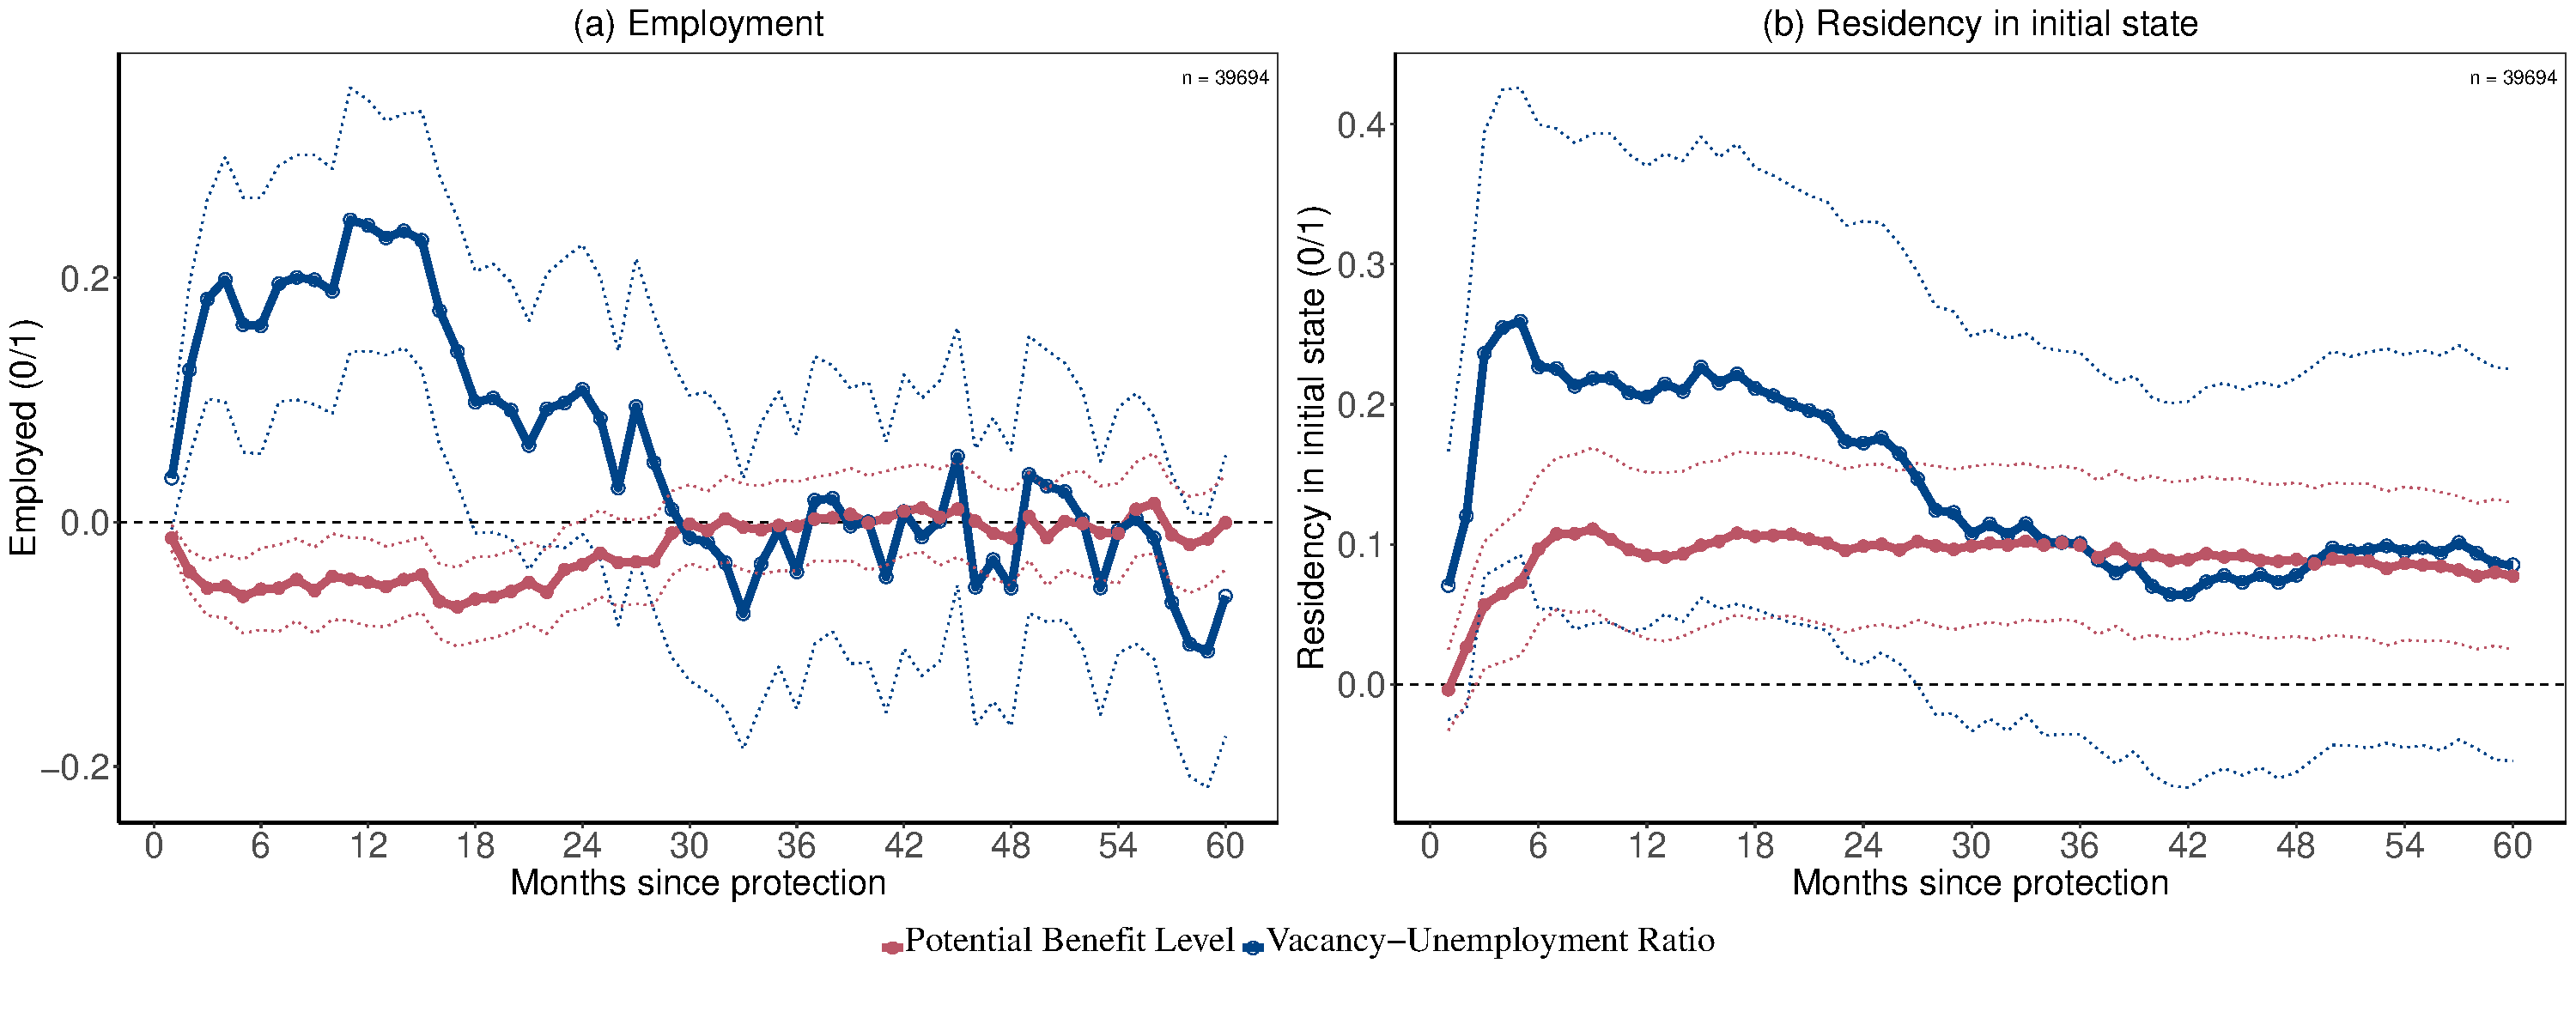
\includegraphics[scale=0.31]{figures/rob/fig_rob_labor_mobility_non_seasonal.pdf}
    \end{center}
    \fignote{\footnotesize \textit{Notes:} The x-axis shows the months since protection was received. The y-axis displays the effect of a one-unit increase in either i) the occupation-specific vacancy-to-unemployment ratio or ii) the potential benefit level, measured in €1,000 (real 2015 values), on employment (left) and mobility (right). All regressions include a full set of arrival-group, year-month, and district-of-protection fixed effects. Additional control variables include age and age squared at immigration, gender, type of protection, family status at protection date, and country of origin. Standard errors are clustered at the state-year-of-protection level.}
\end{figure}





\vspace{0.5cm}
\noindent\textbf{Comparison with concurrent single-sector studies.}\hspace{0.5cm} Two concurrent papers exploit the same Austrian dispersal setting but focus on single labor-market segments. \citet{degenhardt2025initial}, exploiting within-region, within-year seasonal variation in a hospitality-sector vacancy-to-unemployment ratio, finds an initial employment gain of up to 3 percentage points that diminishes after the first year, alongside positive cumulative earnings over three years and increased labor market segregation---complementary to our seasonal-occupations analysis above. \citet{degenhardt2025} use the geographic expansion of online food delivery firms as a low-barrier work treatment, finding that gig availability accelerates initial job-finding but traps workers in low-paid, unstable jobs, with negative effects on human capital and job search. Our general $IVUR$ measure nests these sectoral exercises in a single framework, finds a similar qualitative pattern with a longer fade horizon (around 30 months), and additionally jointly identifies the role of welfare benefit generosity.

\vspace{0.5cm}
\noindent\textbf{Benefit cuts and political decisions as confounder.}\hspace{0.5cm}
In our analysis, we exploit variation in benefit levels across states and refugee types (i.e., singles vs. families). One potential concern is that these benefit cuts may result from political decisions. For instance, more immigration-skeptical parties might attempt to reduce perceived "pull factors" by reducing benefit levels. If this is the case, then political decisions or ideology would be confounding our results and the effects of $IPBL$ would be upward-biased. 

To address this concern, we control for political sentiment using state-level voting intentions for the FPÖ---a far-right populist party---measured at the time of asylum approval. We gathered information on the voting intentions for the FPÖ from various polls as a proxy for the political sentiment in the states at the time when refugees received labor market access.

Figure \ref{fig:fpo} shows the results. Including the FPÖ vote share intentions as a control does not significantly affect the effects of $IPBL$ on employment and mobility.
However, the estimated effect of $IVUR$ on remaining in the initial state is halved compared to our main specification. This suggests that political sentiment might be a bad control for $IVUR$. If labor demand affects political preferences, then the FPÖ vote shares may themselves directly be affected by our variable of interest $IVUR$. 


\begin{figure}
    \caption{Robustness: Controlling for FPÖ Vote Share at Asylum Approval}
    \label{fig:fpo}
    \begin{center}
    \vspace{-0.5 cm}
    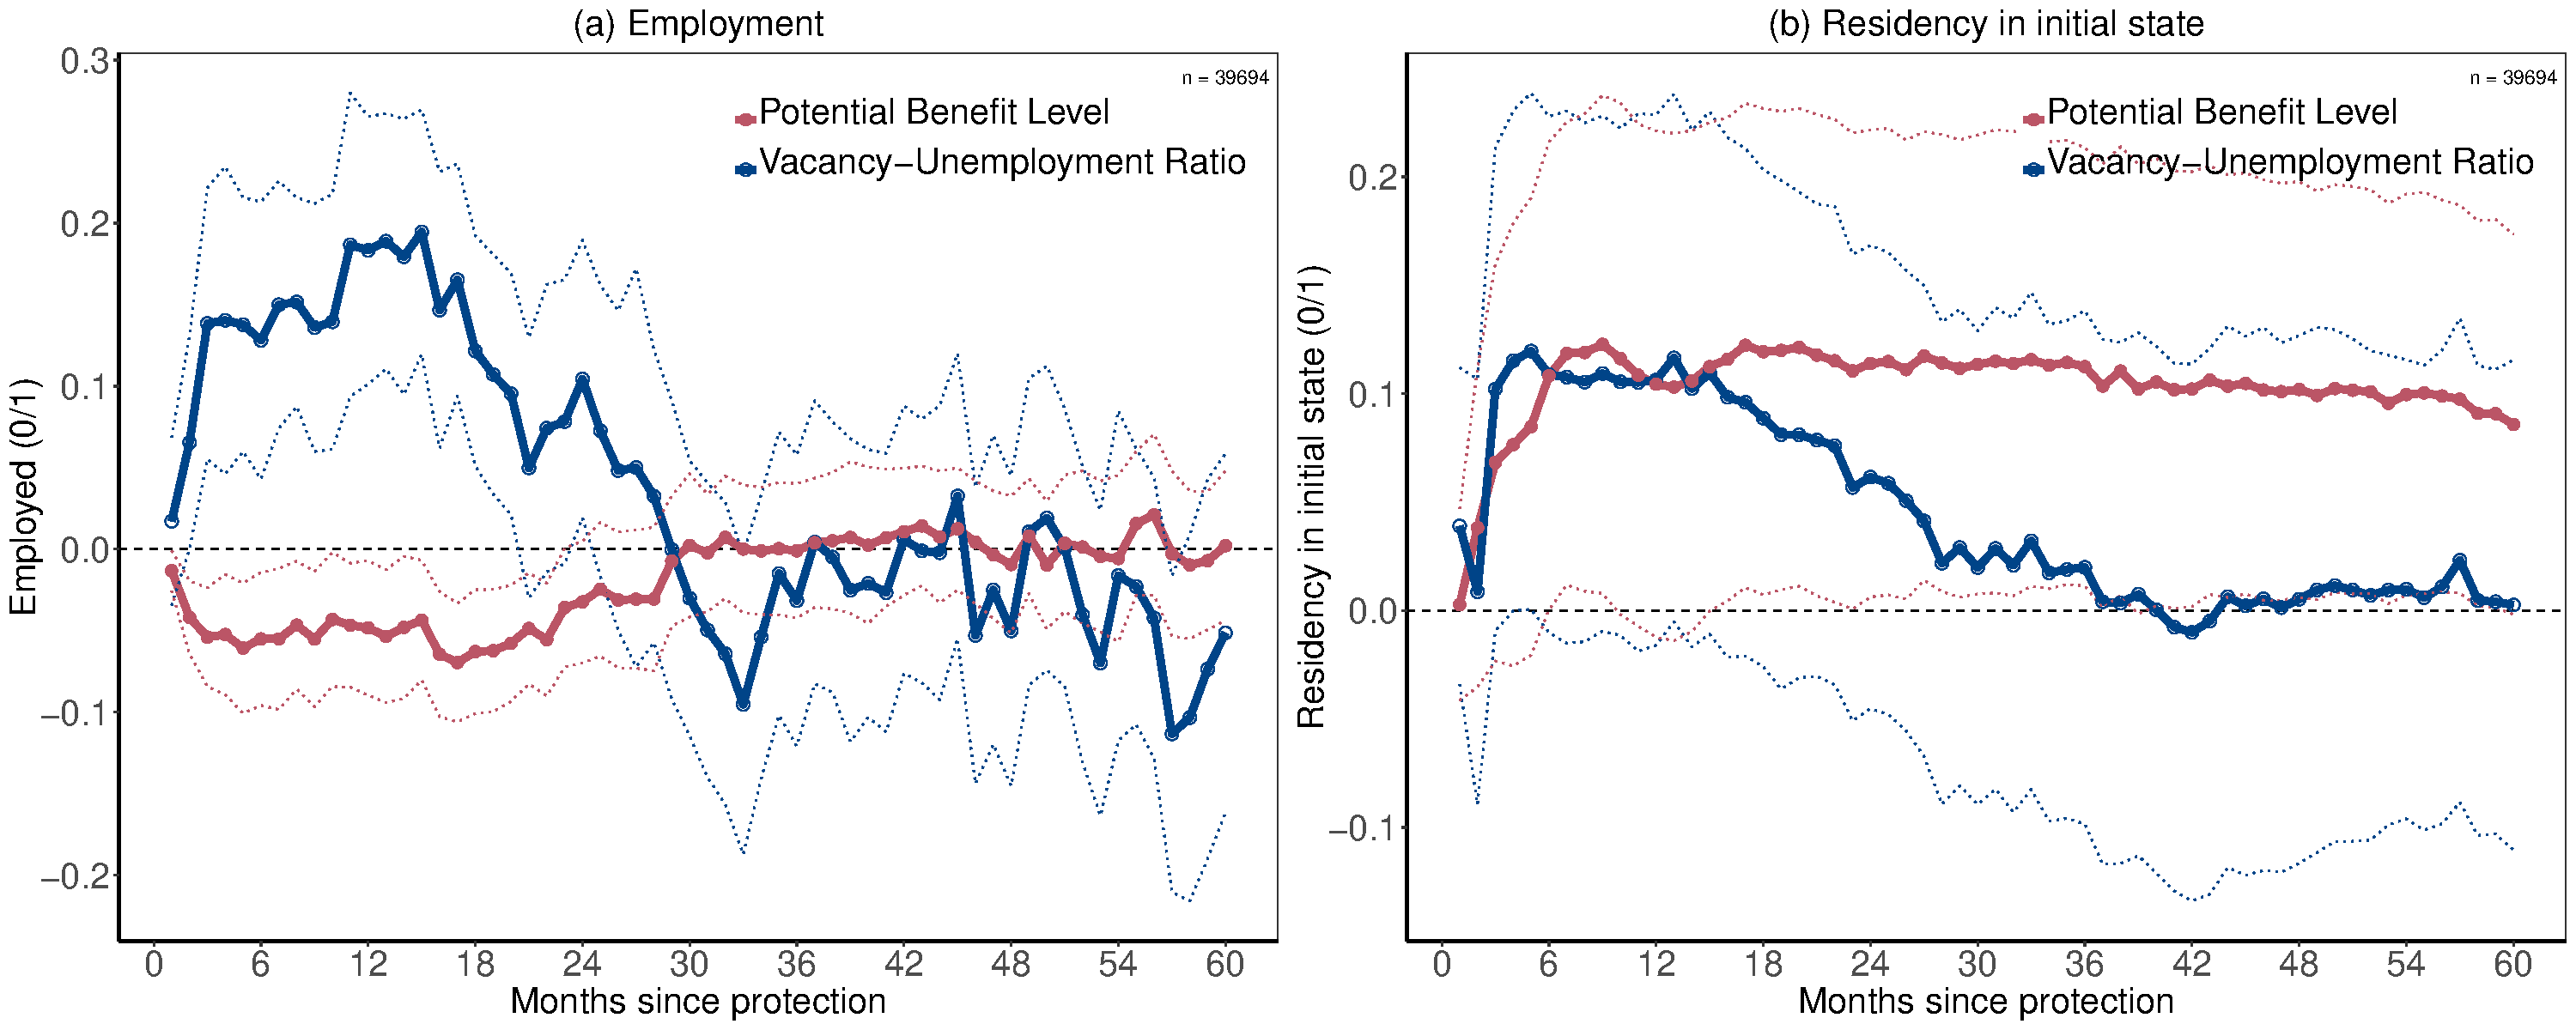
\includegraphics[scale=0.31]{figures/rob/fig_fp_share.pdf}
    \end{center}
    \vspace{-0.5 cm}
    \fignote{\footnotesize \textit{Notes:} The x-axis shows the months since protection was received. The y-axis displays the effect of a one-unit increase in either i) the vacancy-to-unemployment ratio or ii) the potential benefit level, measured in €1,000 (real 2015 values), on selected outcomes. The panels show the effects on (a) having any part- or full-time employment (binary) and (b) on the probability of living in the state of protection. All regressions include a full set of fixed effects for arrival group, year-month, and district of protection. Additional control variables include the FPÖ vote share at the state level at the time of protection, age and age squared at immigration, gender, type of protection, family status at protection date, and country of origin. Standard errors are clustered at the state-year-of-protection level. Dashed lines indicate 95\% confidence intervals.}
\end{figure}

\FloatBarrier
\subsection{Robustness}\label{subsec:robustnessoob}
We perform several robustness checks to assess the sensitivity of our results to various sample restrictions and different specifications. 

For our main specifications, we limited our sample to people who have been observed for a full 60 months. Since our data covers refugees who received protection up to August 2023, we can run our estimations with an extended sample, though the sample composition then changes with the outcome horizon.
Figure~\ref{fig:robustness_asylum2021} presents the results of our main findings without the restriction of being observed for 60 months. By including all refugees who received protection up to the start of 2021, our sample size increases to 45,666 individuals. The coefficients remain mostly unchanged, and the 95\% confidence intervals become slightly narrower for earlier months.

Second, we only consider refugees for whom we can determine in our data that they were in an initial reception facility at the beginning of their stay in Austria. For this group of 13,020 individuals, the assumption of exogenous placement is particularly credible. Figure~\ref{fig:rob_labor_mobility_initial_facility} shows the main results for this sample. Again, the overall patterns remain similar, with the effects of $IPBL$ on employment being somewhat smaller in magnitude.

In a related spirit, we exclude individuals who received protection within one month after first registering in Austria. This unusually quick process might still hint at individuals who came via family reunification.\footnote{In the main specification, we exclude individuals who received protection on the same day as they registered in Austria.} This tighter restriction excludes 2,036 observations, leaving a sample of 37,658 observations. However, results remain virtually unchanged (see Figure~\ref{fig:rob_labor_mobility_process_more1month}).

Third, we exclude individuals who received protection within four months of any of the welfare reforms. For these individuals, the $IPBL$ treatment is hard to interpret, as their benefit level changes immediately before/after receiving protection. As this concerns only 674 individuals, results hardly change from the main specification (see Figure~\ref{fig:rob_labor_mobility_noreform_4month}).

Fourth, we exclude individuals who moved between states in the month before receiving protection. This concerns 6,428 individuals. We suspect that these individuals already knew about the imminent granting of a protection status and moved preemptively. Figure~\ref{fig:rob_labor_mobility_state_approval_min1month} shows that excluding these observations leaves the results practically unchanged.

Fifth, we examine the robustness of inference to alternative clustering levels. Figure~\ref{fig:errors_all} shows 95\% confidence intervals at six choices: commuting zone, district, district $\times$ year, state, state $\times$ year-of-protection (our headline), and a wild-cluster bootstrap with Webb weights to address Austria's small number of states (nine). The two treatments vary at different aggregations---$IVUR$ at the district $\times$ month level, $IPBL$ at the state $\times$ protection-type $\times$ family-status $\times$ month level---and our headline state $\times$ year-of-protection cluster sits between these. It captures within-cohort residual correlation in placement, asylum-processing timing, and state-level policy environment. Under the wild-cluster bootstrap, which is the small-N-conservative choice with only nine states, confidence intervals widen and the band for the $IPBL$ effect on employment approaches zero at most horizons. We read this not as evidence that the $IPBL$ effect on employment is spurious but as a reminder that the statistical strength of that particular estimate is moderate; the $IPBL$ effect on mobility and the $IVUR$ effects throughout remain clearly distinguishable from zero across all clustering choices.

To ensure a particular nationality or state does not drive our results, we re-estimate the effects by systematically excluding either one nationality at a time (Figure~\ref{fig:leavenats}) or one state at a time (Figure~\ref{fig:leavestates}) in our main specification. In the leave-one-nationality-out analysis, the estimated effects remain largely unchanged, indicating robustness across different nationalities.
For the leave-one-state-out analysis, we modify our main specification by including an additional interaction of eligibility-for-family-benefits*state*type-of-protection. This adjustment is necessary since---otherwise---we would be using variation stemming from differences between refugee status (Convention vs. subsidiary protection) and eligibility for family benefits across states.  
Again, we see little change in our main results. If anything, the effects on mobility are larger when excluding Upper Austria (upper blue line) and are halved when excluding Vienna (lower blue line), likely due to the high concentration of refugees in this city.   

Finally, we use separate month and year-of-protection fixed effects instead of year-month fixed effects. This modification does not alter the results meaningfully (see Figure~\ref{fig:rob_labor_mobility_year_month_fe}).

Overall, we conclude that our results are robust to various changes in the sample and specification.

% \begin{figure}
%     \caption{Descriptive outcomes by moving behavior}
%     \label{fig:descriptive_outcomes_mover_group}
%     \begin{center}
%     \vspace{-0.5 cm}
%     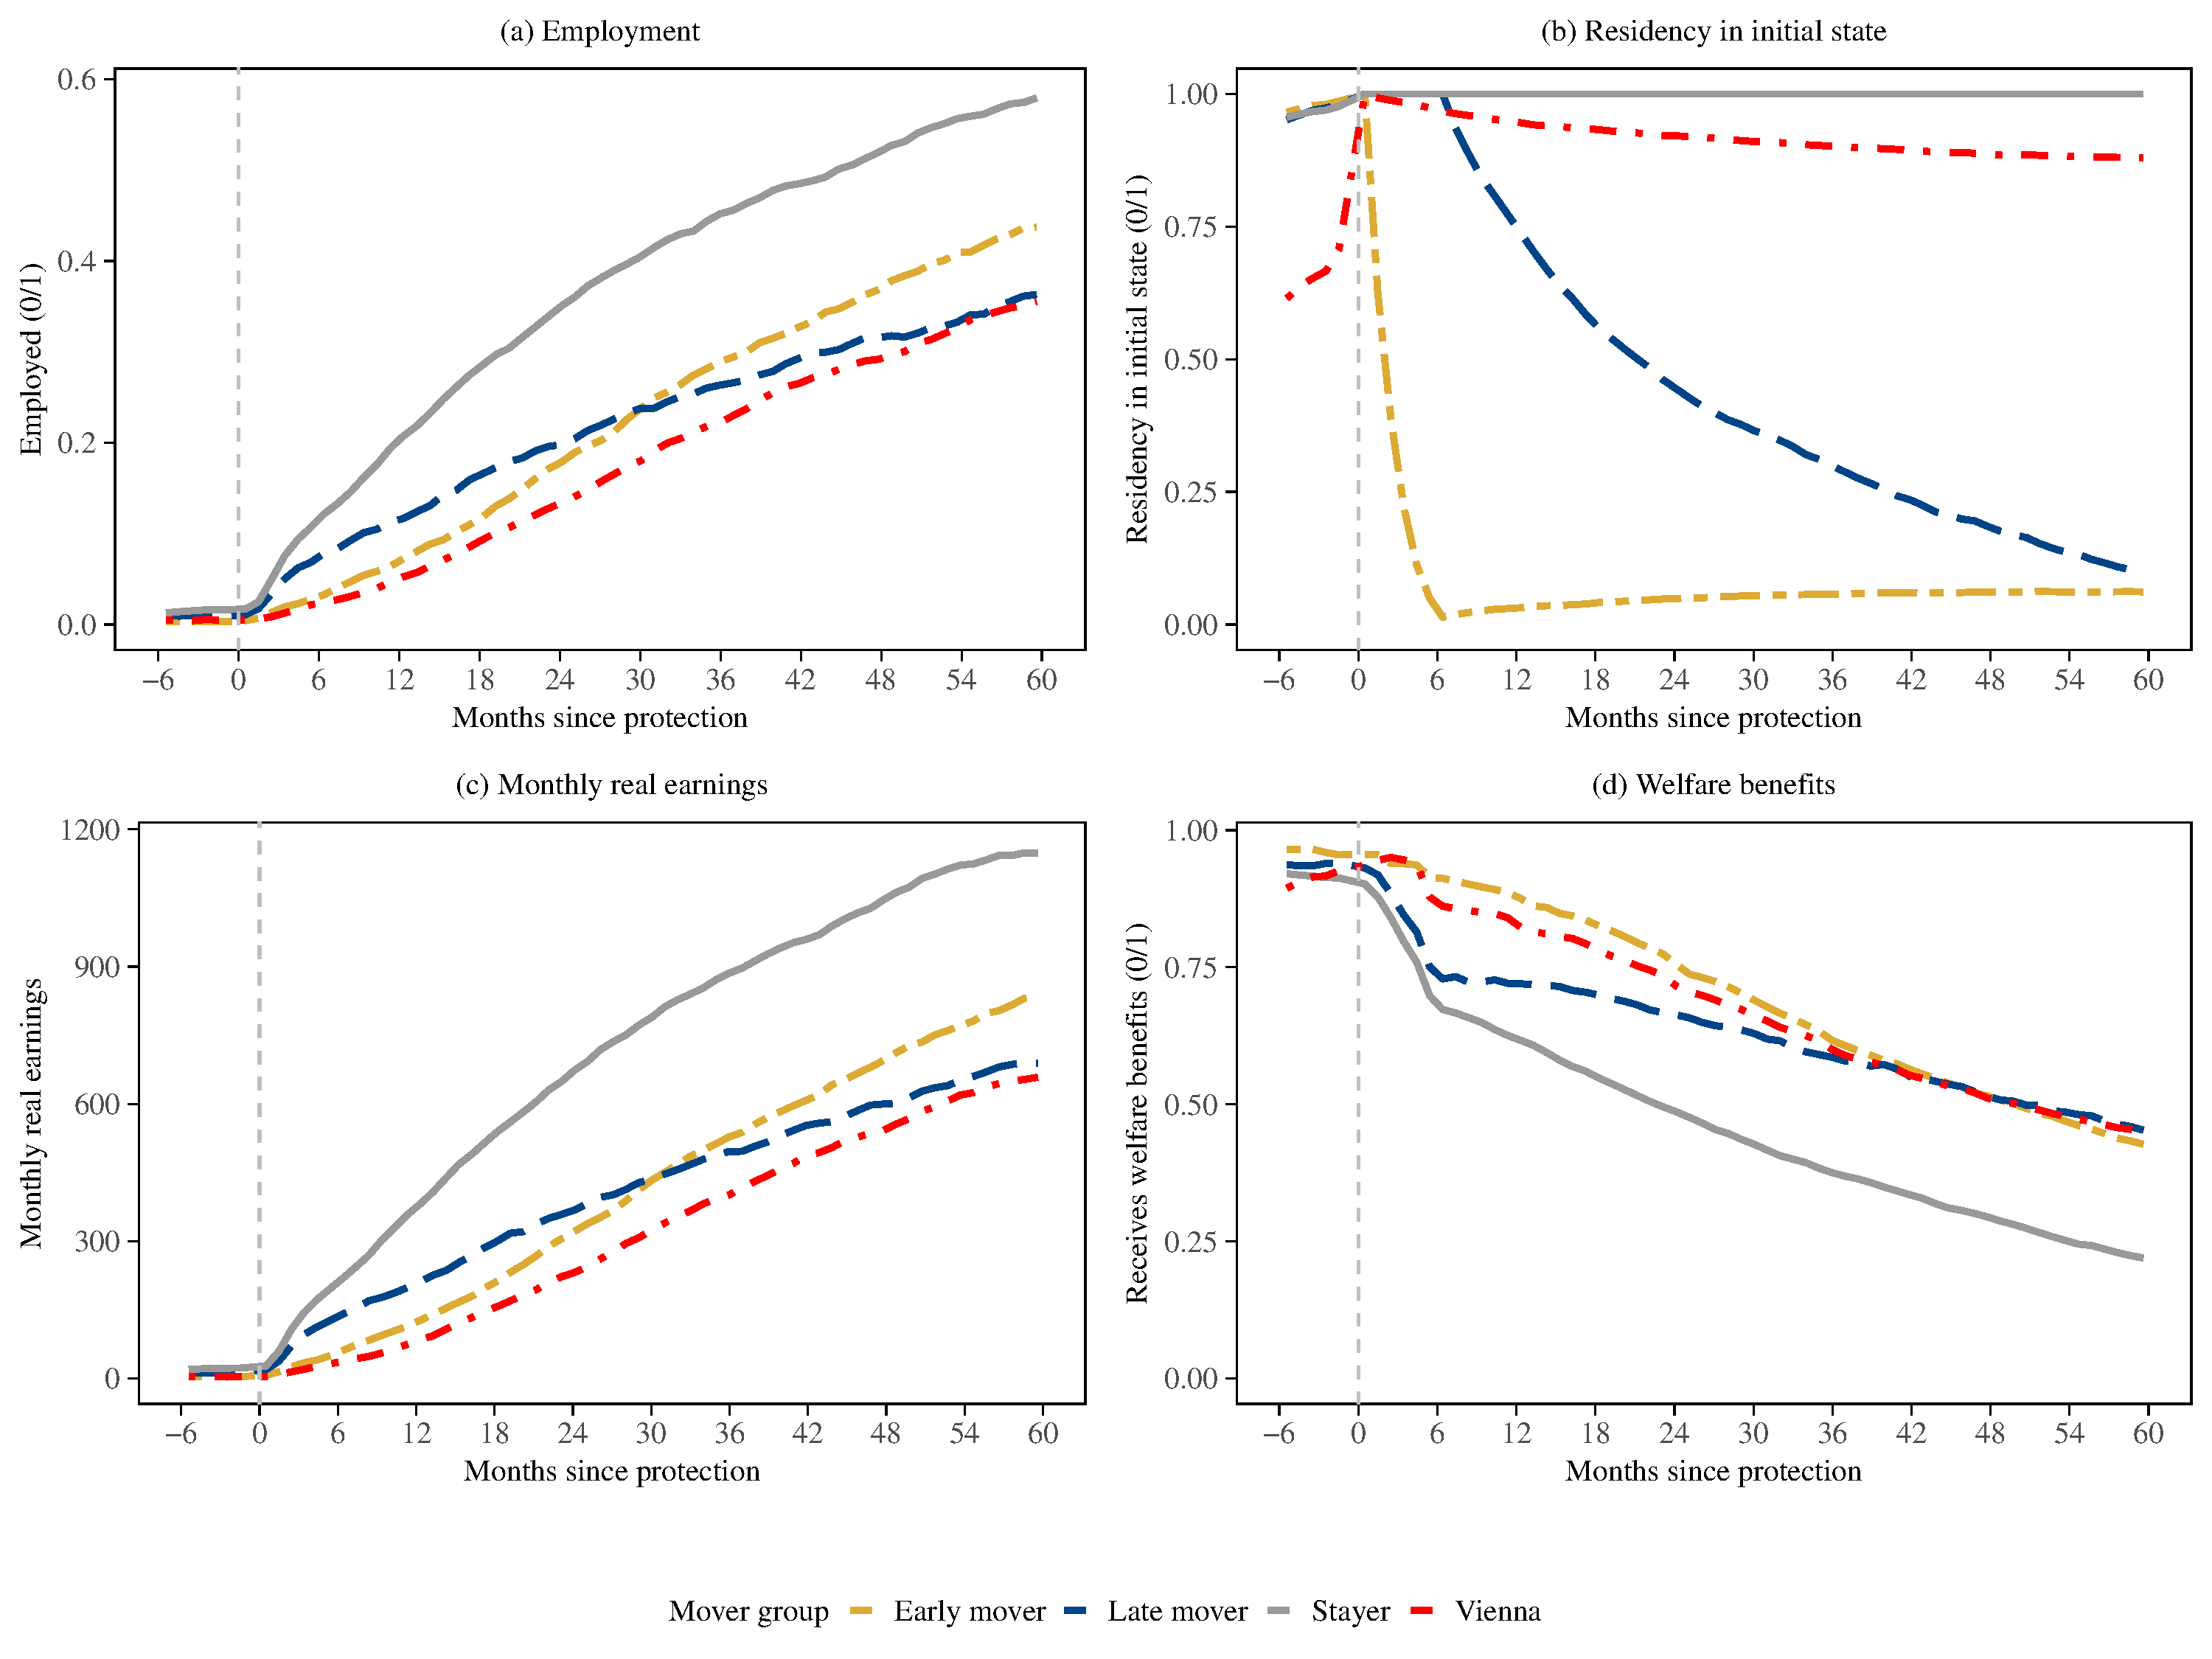
\includegraphics[scale=0.31]{figures/rob/fig_descriptive_outcomes_mover_group.pdf}
%     \end{center}
%     \fignote{Notes: The x-axis shows the months since protection was received. The y-axis displays descriptive outcomes for the groups categorized by their moving behavior.}
% \end{figure}

% \begin{figure}
%     \caption{Descriptive outcomes by moving behavior excluding people with relocation one month prior asylum granting}
%     \label{fig:mover_group_no_early}
%     \begin{center}
%     \vspace{-0.5 cm}
%     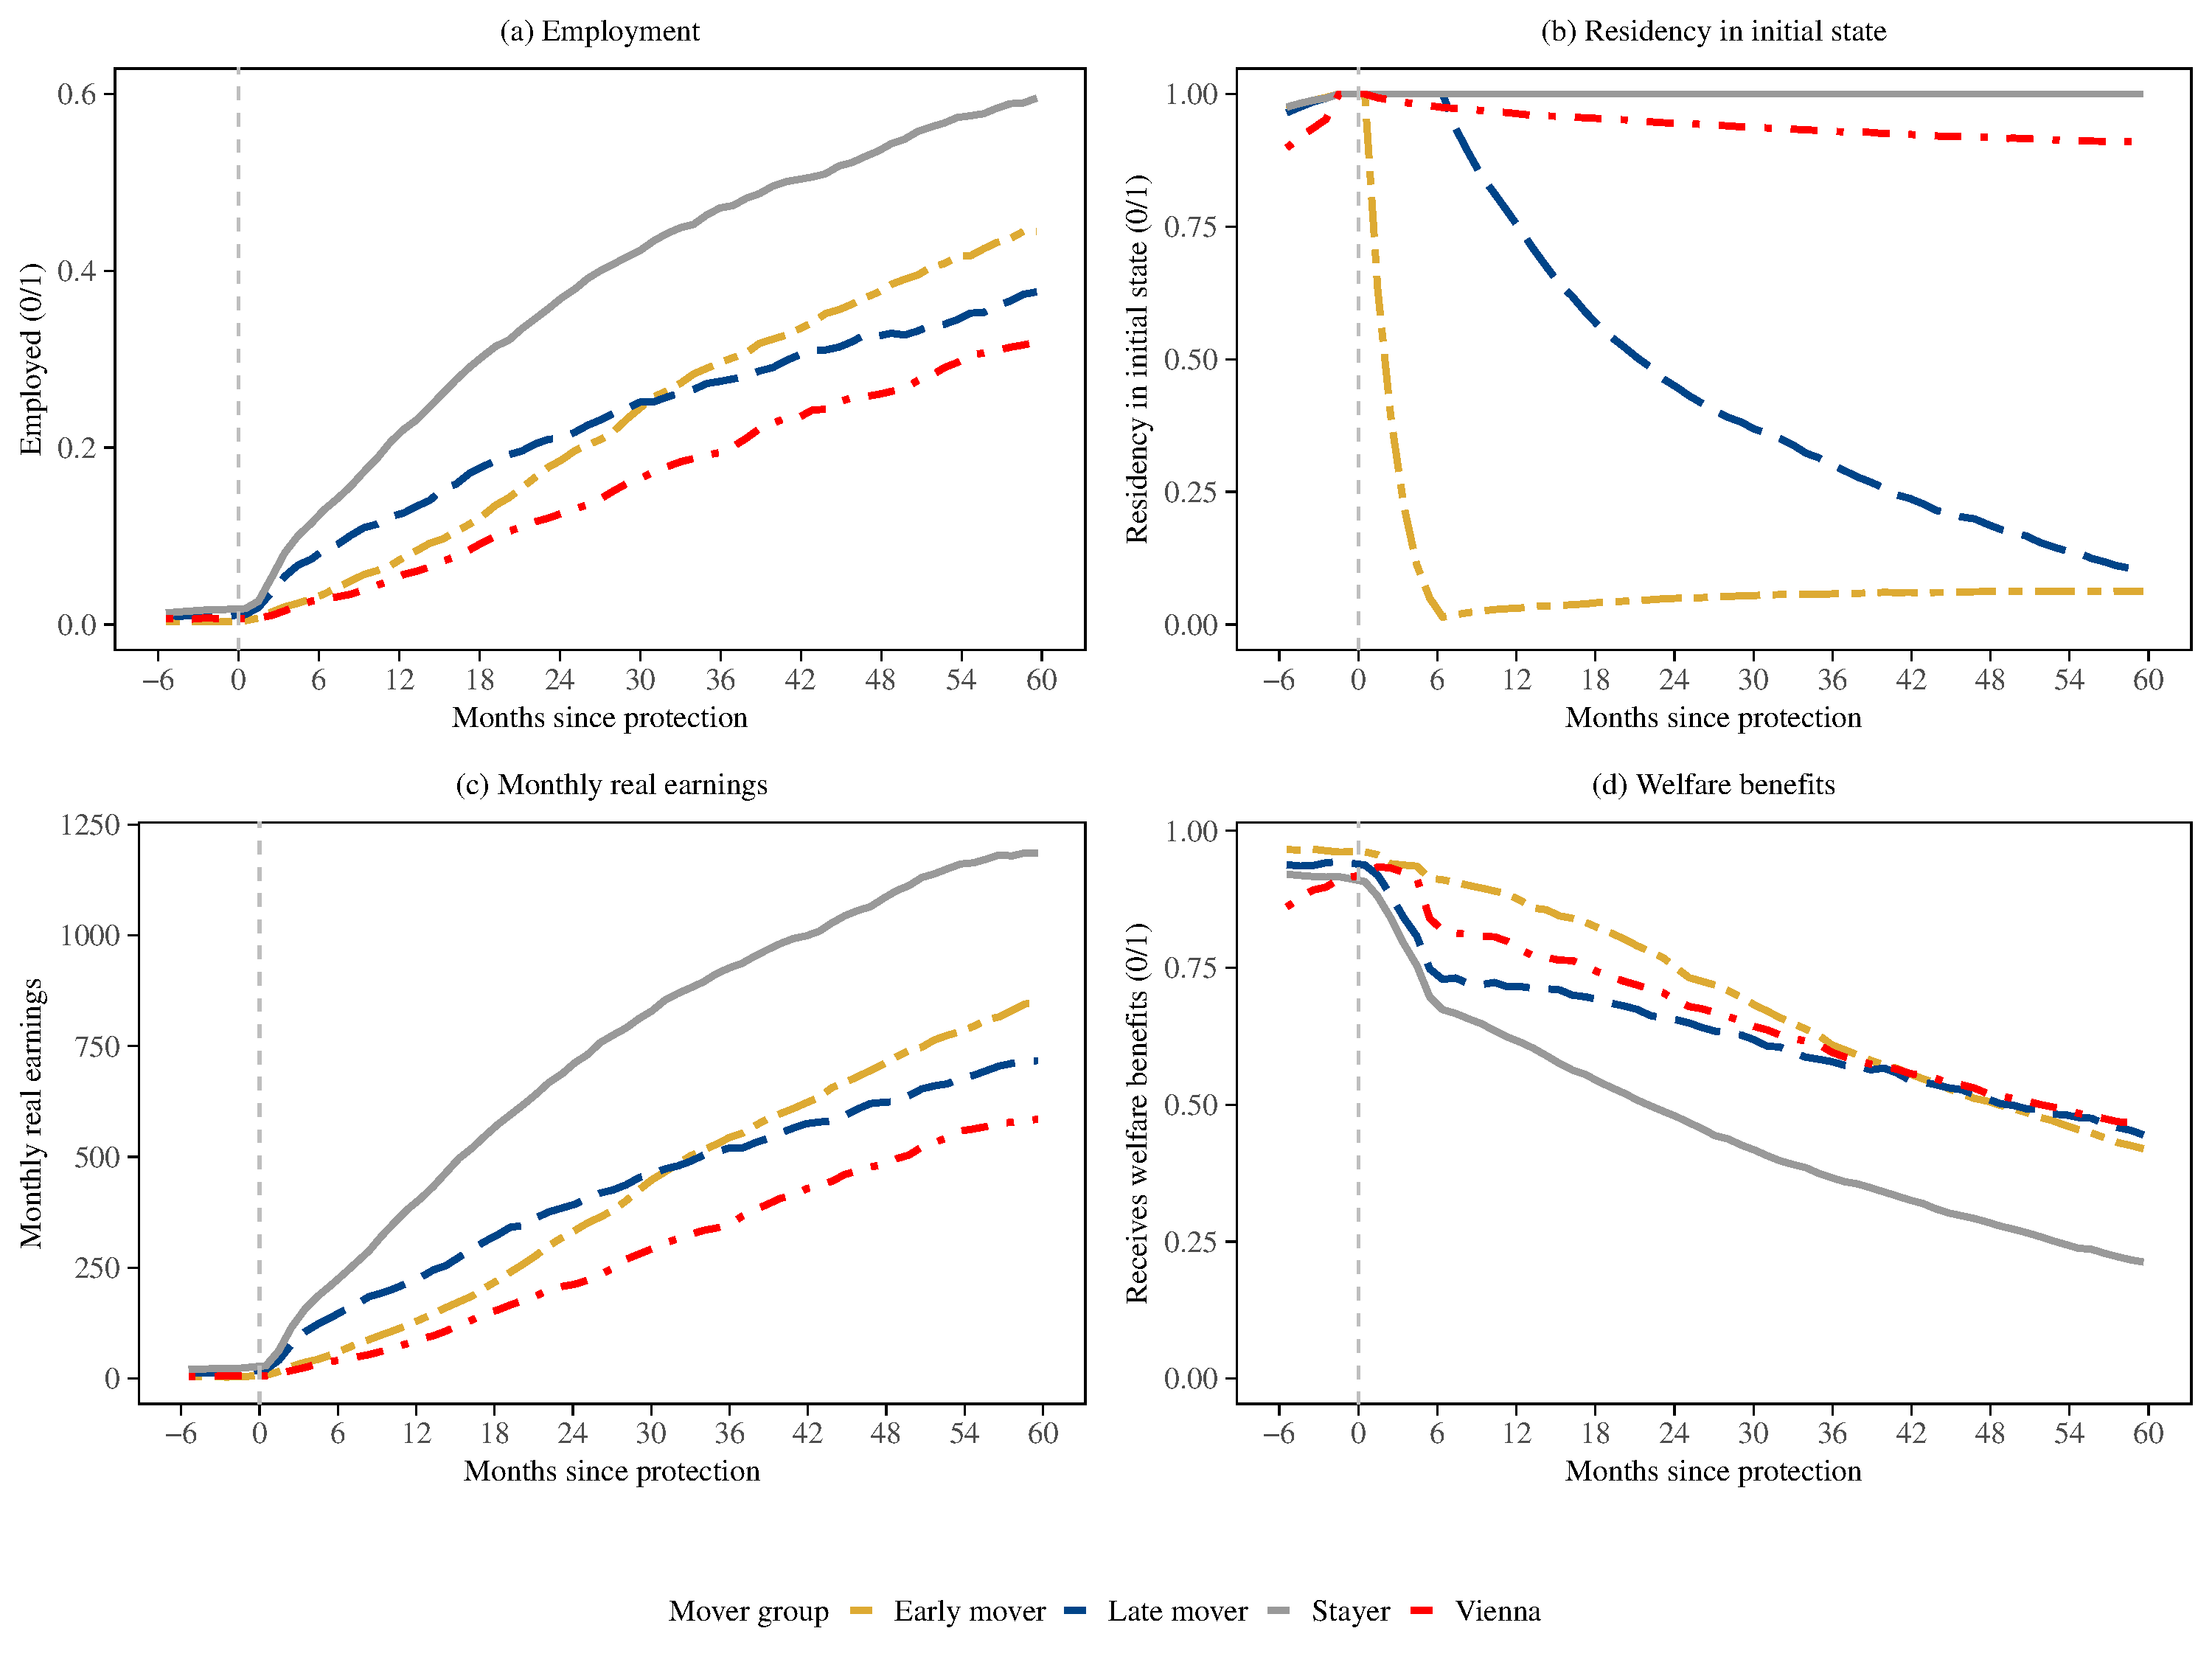
\includegraphics[scale=0.31]{figures/rob/fig_descriptive_outcomes_mover_group_no_early_movers.pdf}
%     \end{center}
%     \fignote{Notes: The x-axis shows the months since protection was received. The y-axis displays descriptive outcomes for the groups categorized by their moving behavior.}
% \end{figure}




% \begin{figure}
%     \caption{Effect of the $IVUR$ and $IPBL$ on employment and location choice with initial residency shifted to one month before receiving asylum}
%     \label{fig:rob_labor_mobility_initial_state_shift1}
%     \begin{center}
%     \vspace{-0.5 cm}
%     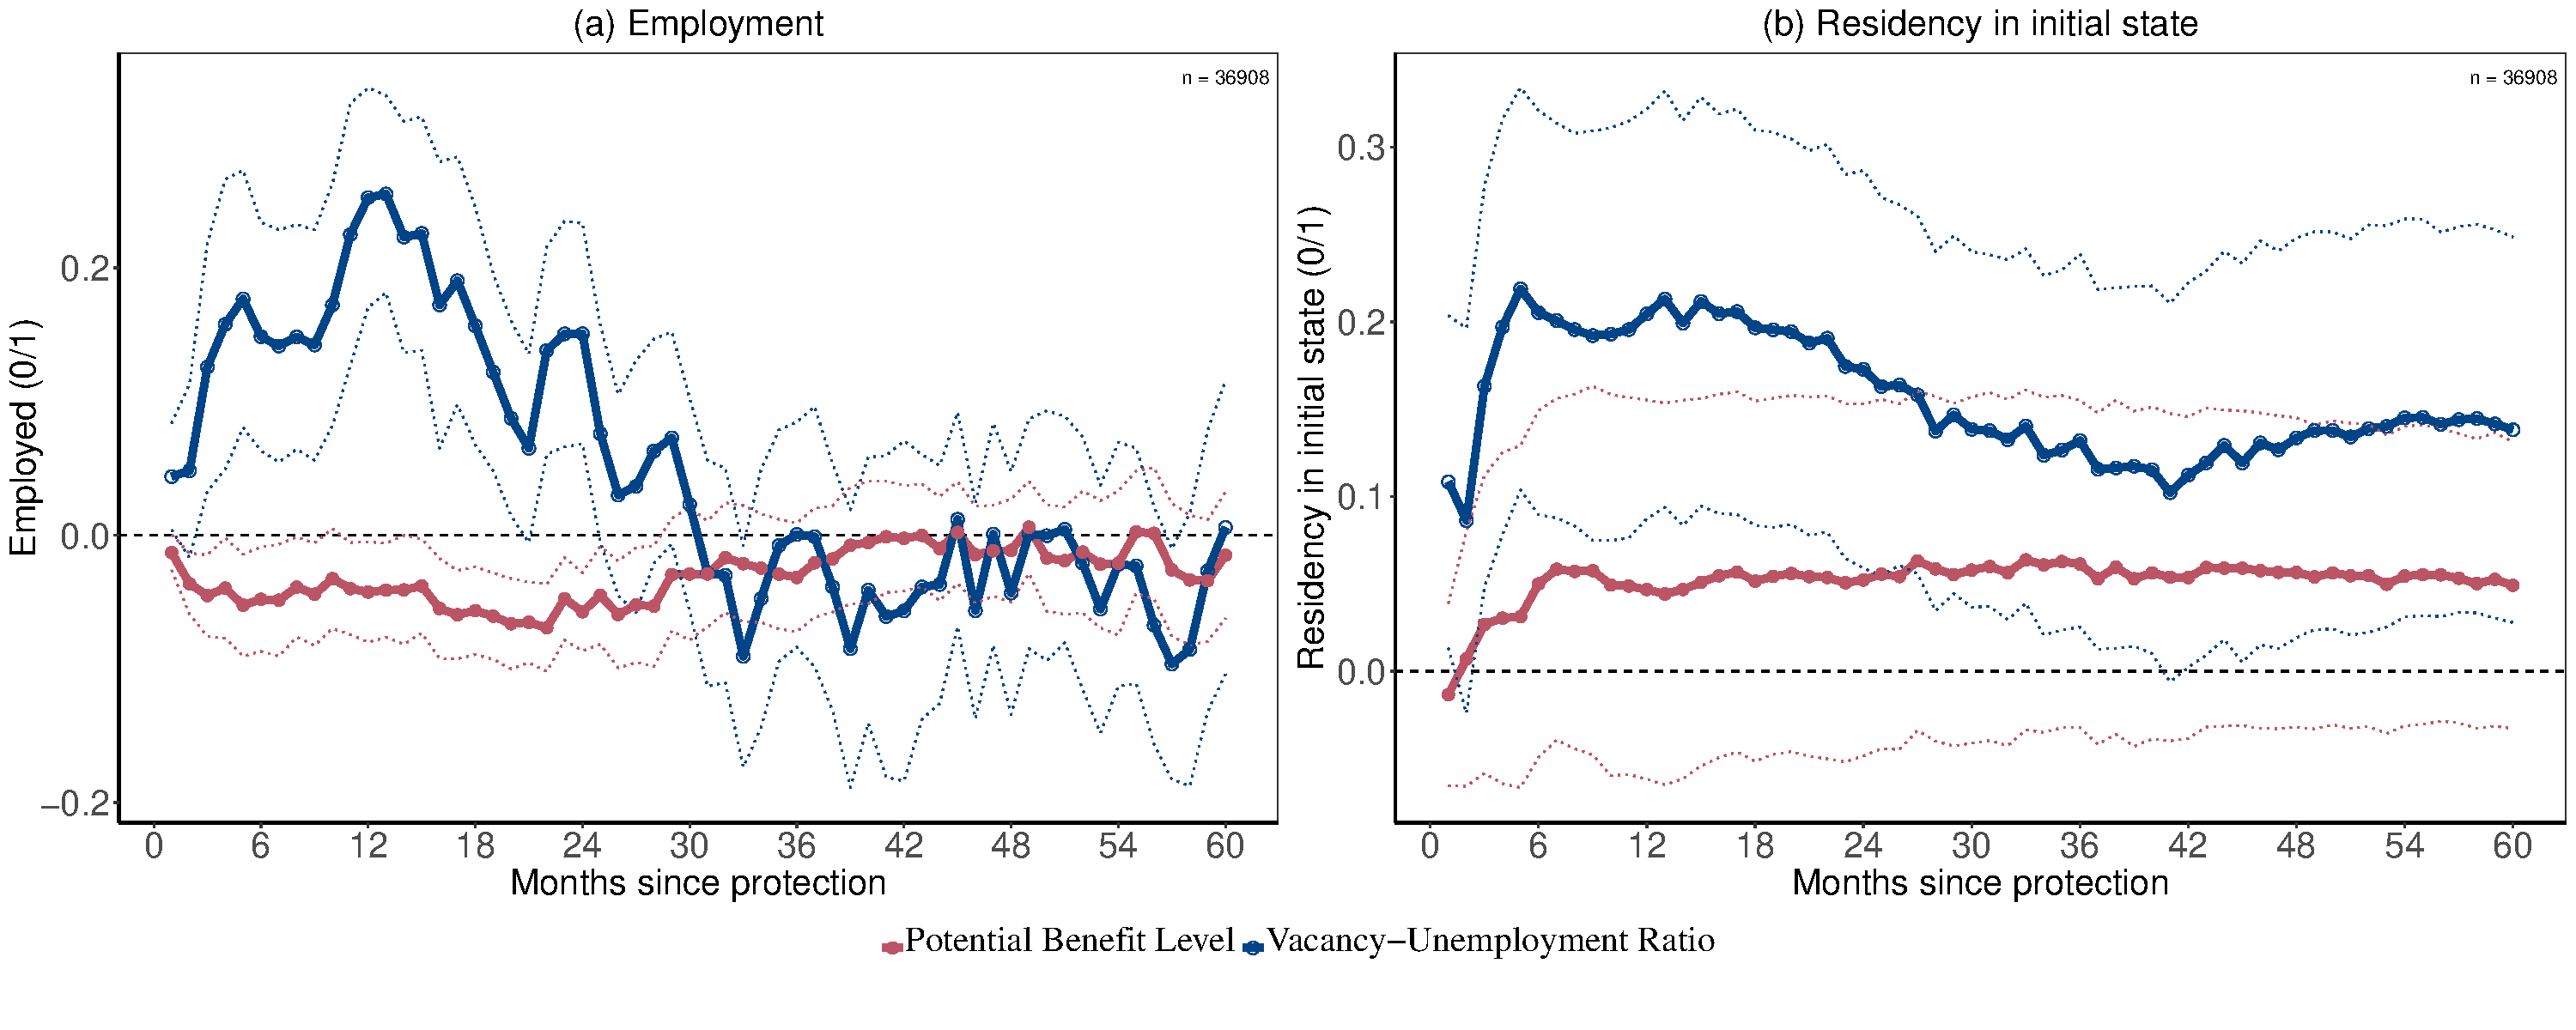
\includegraphics[scale=0.31]{figures/rob/fig_rob_labor_mobility_initial_state_shift1.pdf}
%     \end{center}
%     \fignote{Notes: The x-axis shows the months since protection was received. The y-axis displays the effect of a one-unit increase in either i) the vacancy-to-unemployment ratio or ii) the potential benefit level, measured in €1,000 (real 2015 values), on employment (left) and mobility (right). All regressions include a full set of arrival-group, year-month, and district-of-protection fixed effects. Additional control variables include age and age squared at immigration, gender, type of protection, family status at protection date, and country of origin. Standard errors are clustered at the district-year-of-protection level.}
% \end{figure}


% \begin{figure}
%     \caption{Effect of the $IVUR$  for the most desired professions and $IPBL$ on employment and location choice}
%     \label{fig:rob_labor_mobility_most_desired}
%     \begin{center}
%     \vspace{-0.5 cm}
%     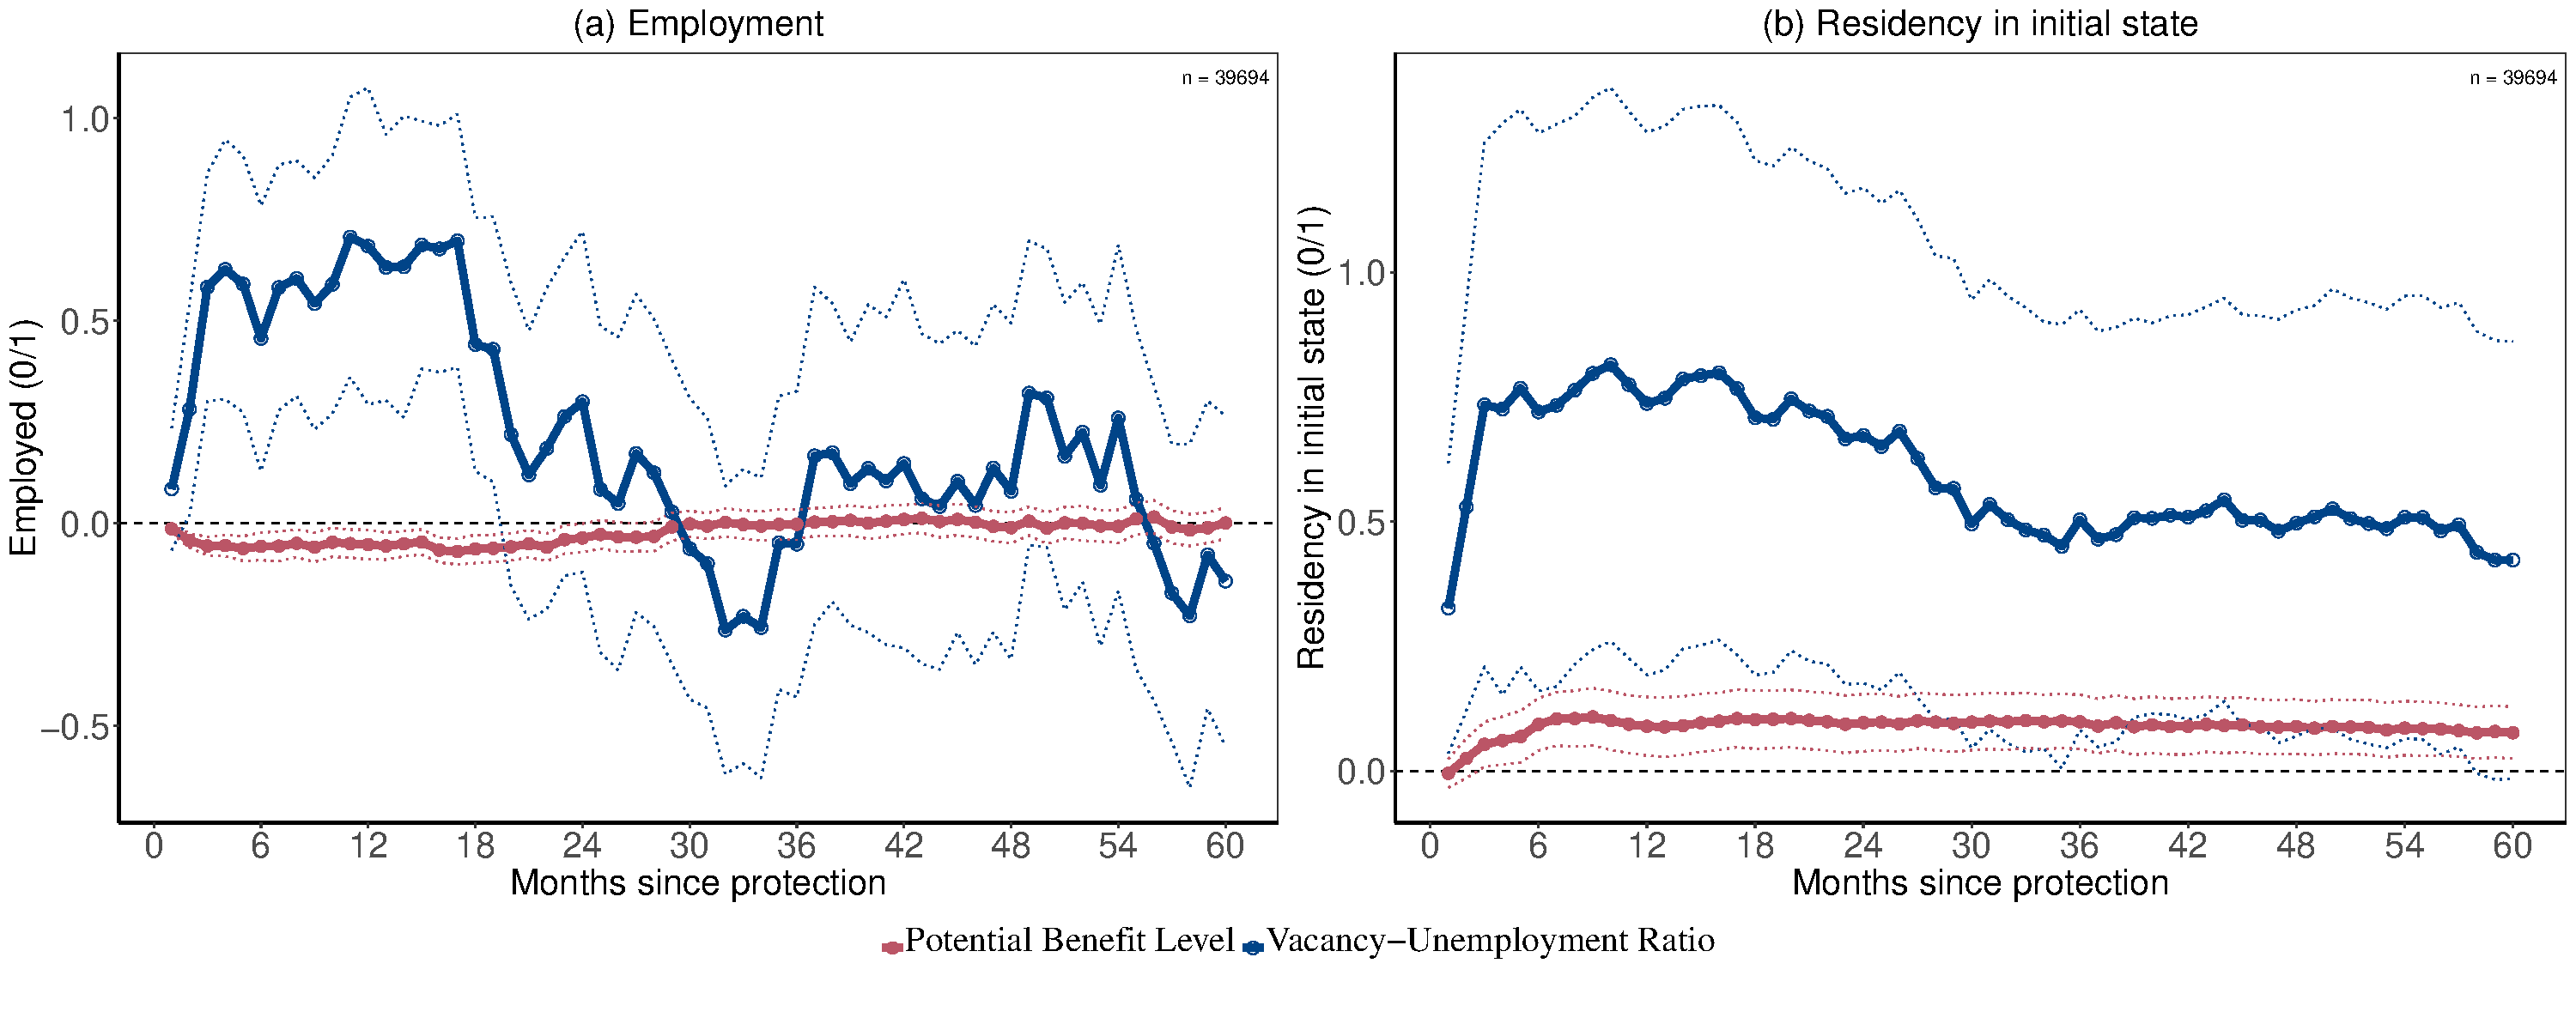
\includegraphics[scale=0.31]{figures/rob/fig_rob_labor_mobility_most_desired.pdf}
%     \end{center}
%     \fignote{Notes: The x-axis shows the months since protection was received. The y-axis displays the effect of a one-unit increase in either i) the occupation-specific vacancy-to-unemployment ratio or ii) the potential benefit level, measured in €1,000 (real 2015 values), on employment (left) and mobility (right). All regressions include a full set of arrival-group, year-month, and district-of-protection fixed effects. Additional control variables include age and age squared at immigration, gender, type of protection, family status at protection date, and country of origin. Standard errors are clustered at the district-year-of-protection level.}
% \end{figure}



% \begin{figure}
%     \caption{Effect of the $IVUR$ for seasonal professions and $IPBL$ on employment and location choice}
%     \label{fig:rob_labor_mobility_seasonal}
%     \begin{center}
%     \vspace{-0.5 cm}
%     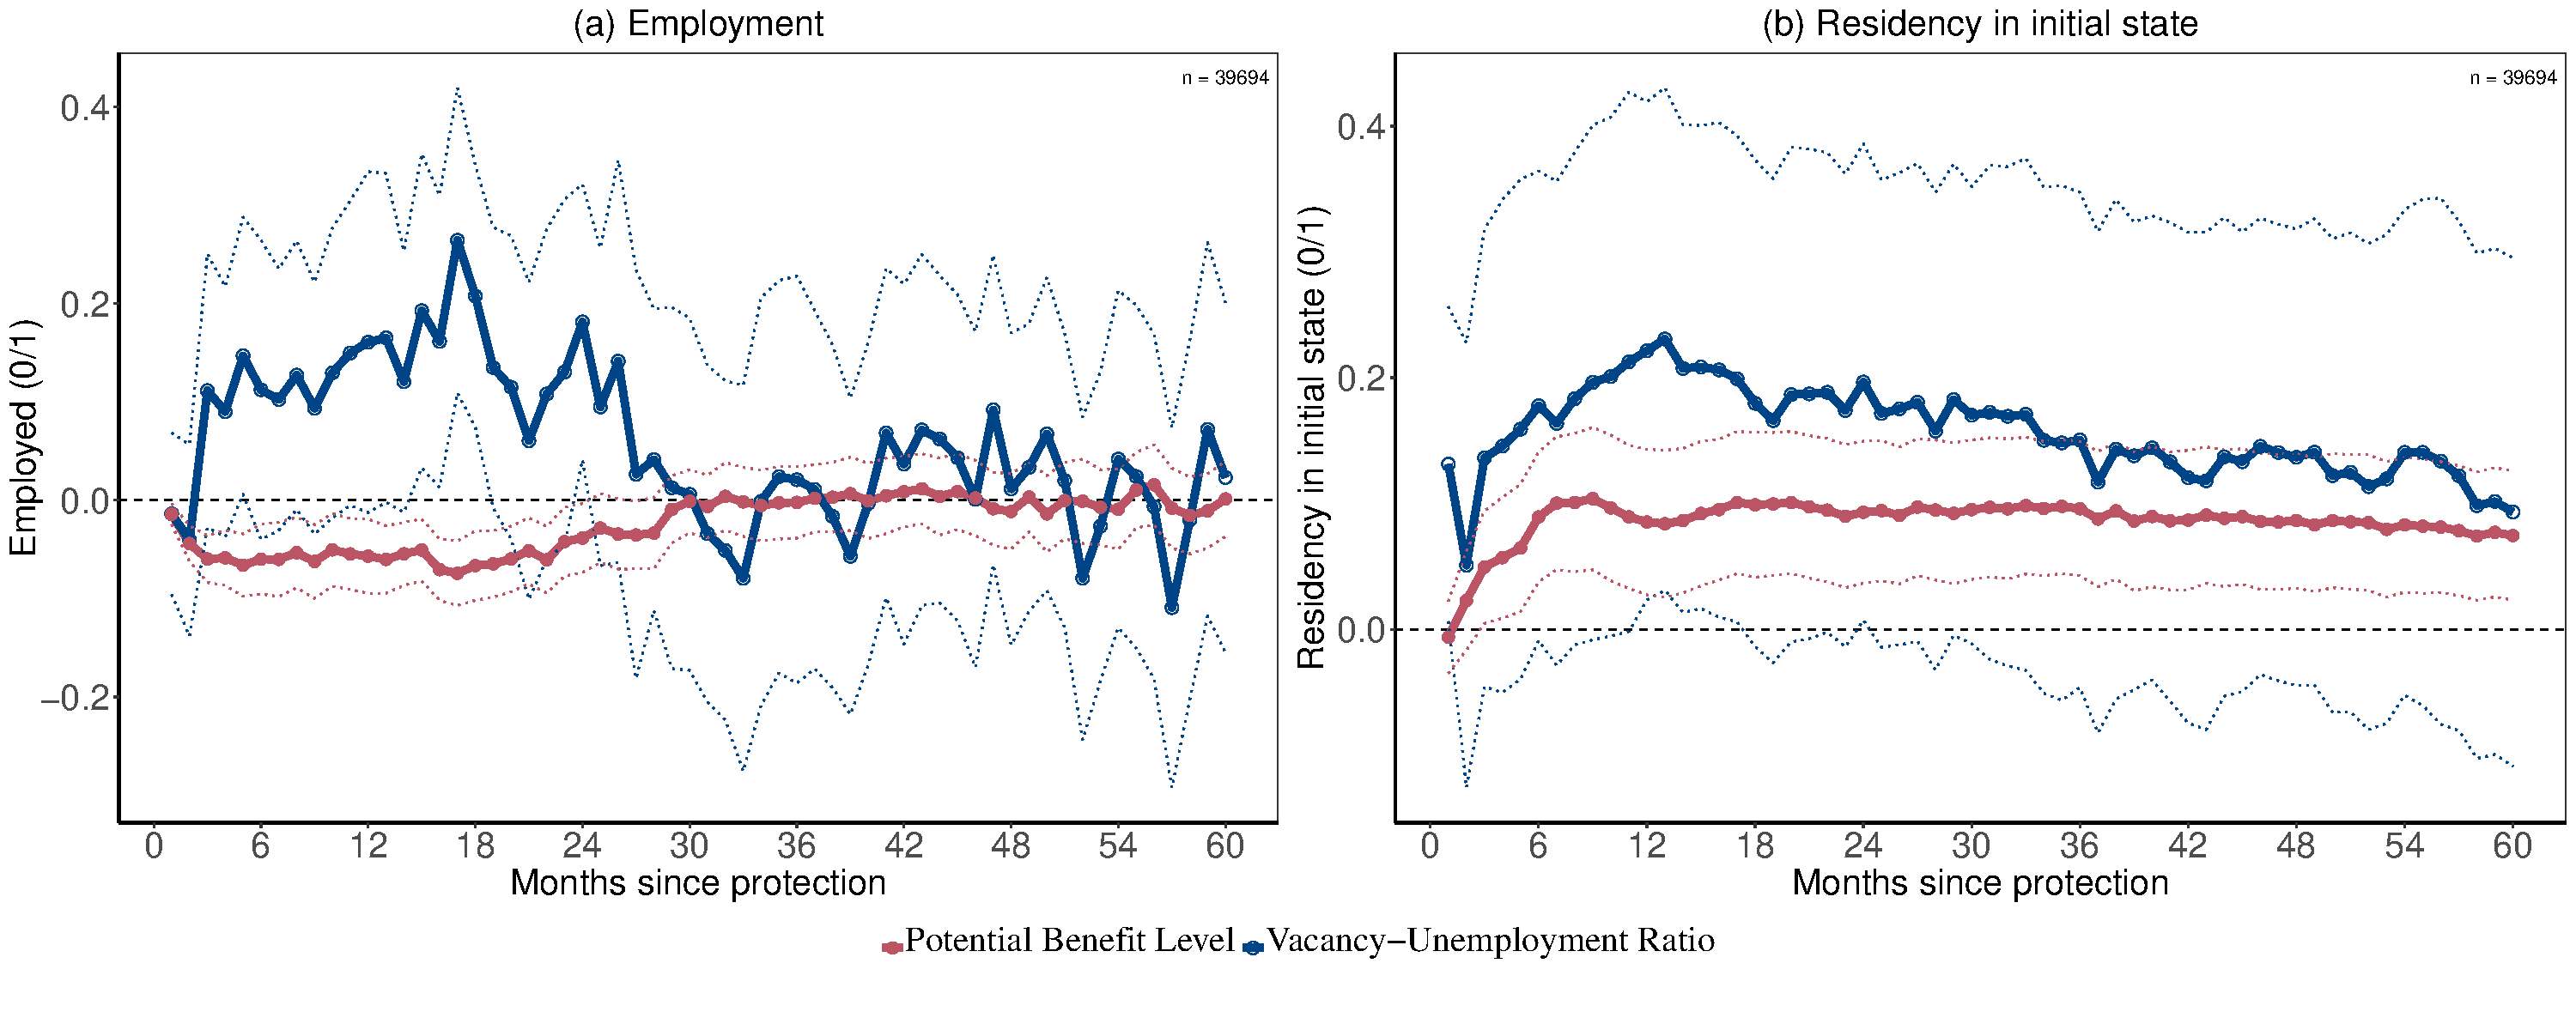
\includegraphics[scale=0.31]{figures/rob/fig_rob_labor_mobility_seasonal.pdf}
%     \end{center}
%     \fignote{Notes: The x-axis shows the months since protection was received. The y-axis displays the effect of a one-unit increase in either i) the occupation-specific vacancy-to-unemployment ratio or ii) the potential benefit level, measured in €1,000 (real 2015 values), on employment (left) and mobility (right). All regressions include a full set of arrival-group, year-month, and district-of-protection fixed effects. Additional control variables include age and age squared at immigration, gender, type of protection, family status at protection date, and country of origin. Standard errors are clustered at the district-year-of-protection level.}
% \end{figure}


% \begin{figure}
%     \caption{Pretrends: Effect of the $IVUR$ and $IPBL$ on employment and location choice}
%     \label{fig:rob_labor_mobility_pre_trends}
%     \begin{center}
%     \vspace{-0.5 cm}
%     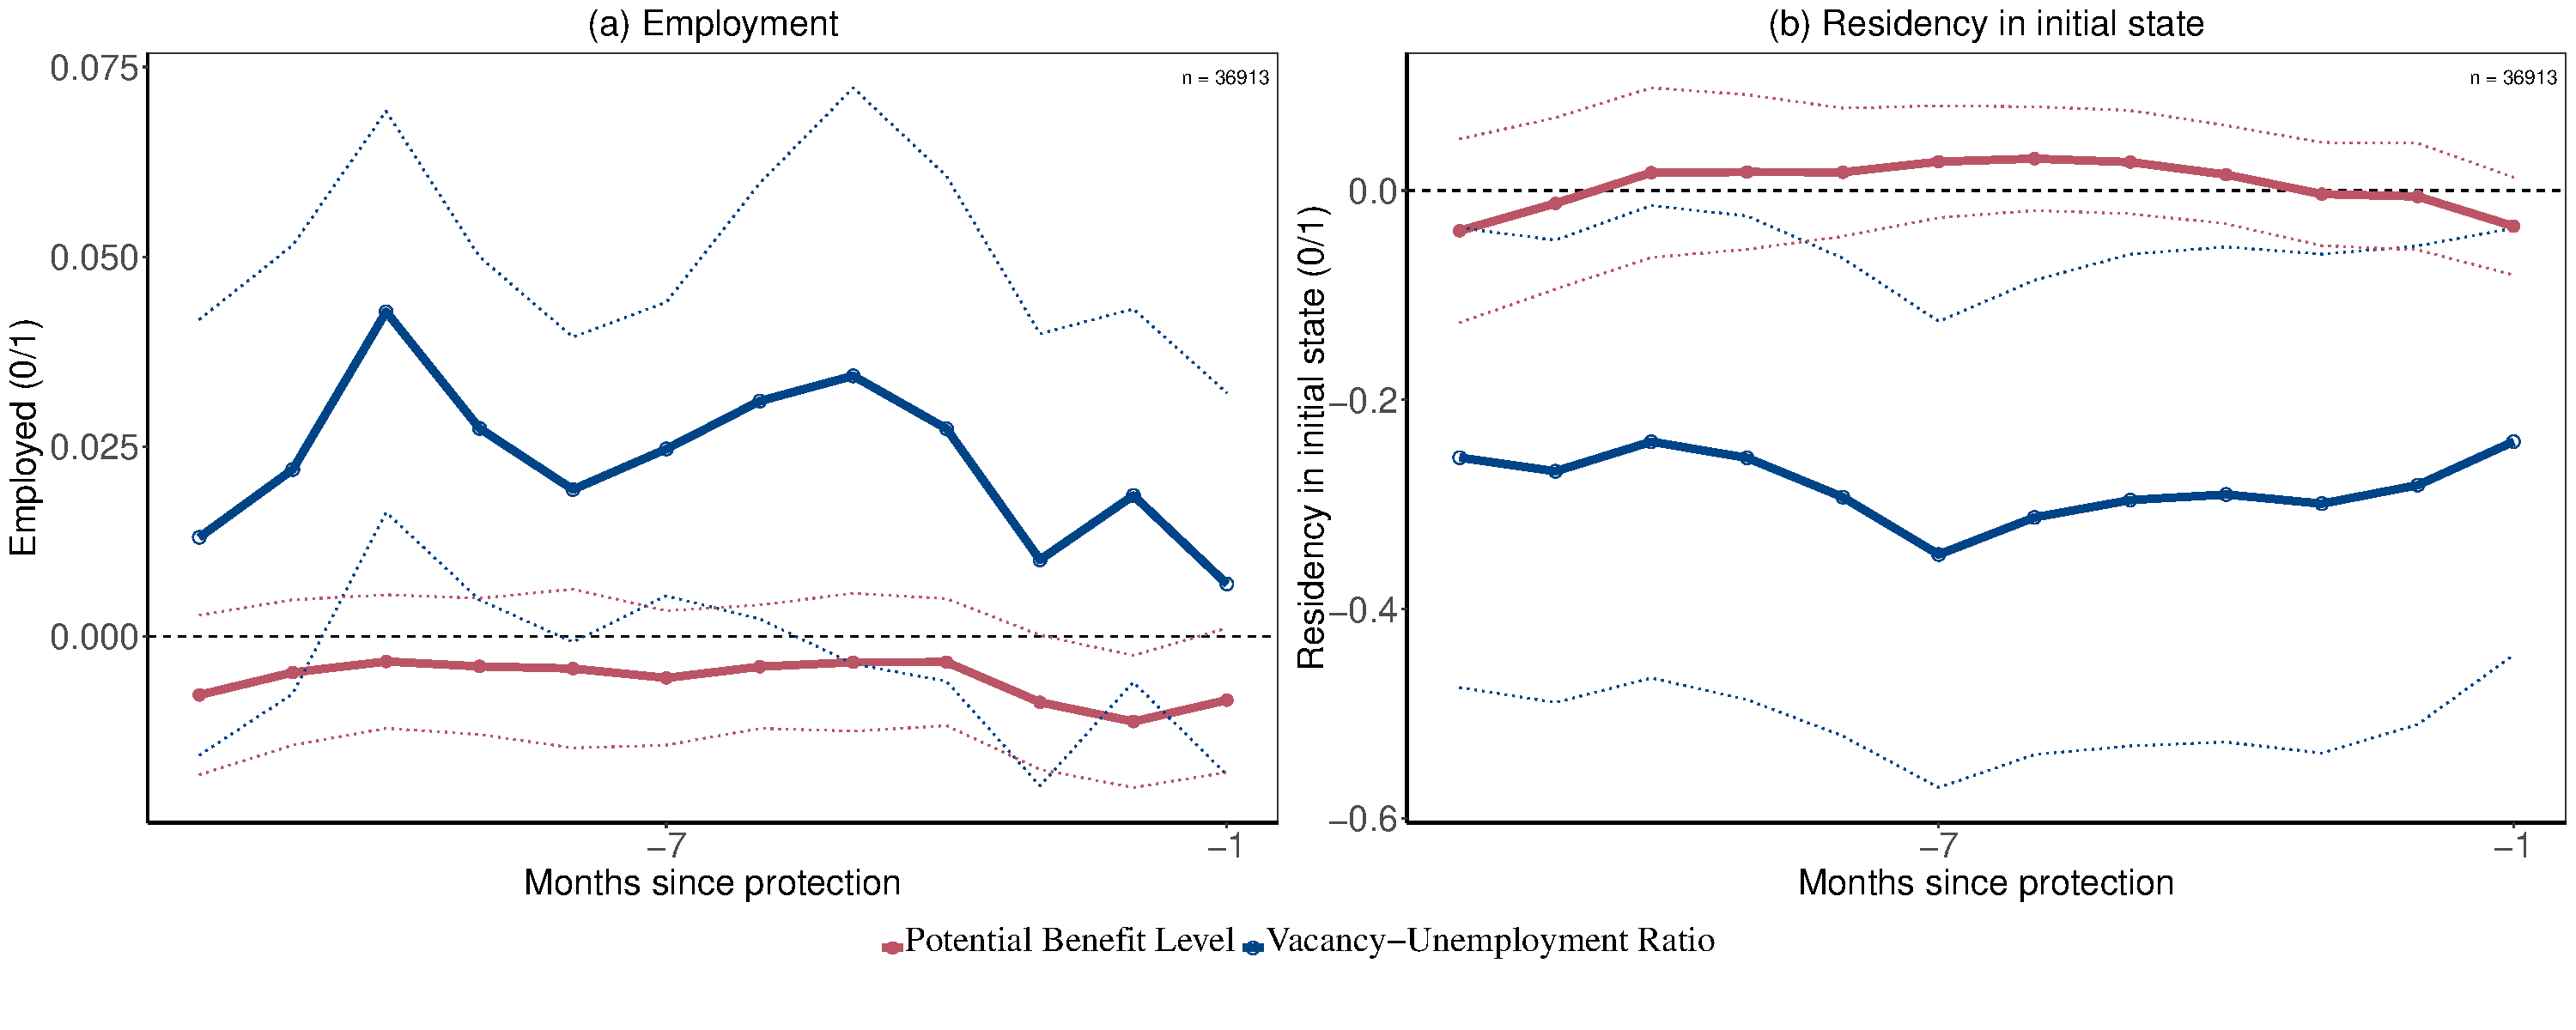
\includegraphics[scale=0.31]{figures/rob/fig_rob_labor_mobility_pre_trends.pdf}
%     \end{center}
%     \fignote{Notes: The x-axis shows the months since protection was received. The y-axis displays the effect of a one-unit increase in either i) the vacancy-to-unemployment ratio or ii) the potential benefit level, measured in €1,000 (real 2015 values), on employment (left) and mobility (right). All regressions include a full set of arrival-group, year-month, and district-of-protection fixed effects. Additional control variables include age and age squared at immigration, gender, type of protection, family status at protection date, and country of origin. Standard errors are clustered at the district-year-of-protection level.}
% \end{figure}

% \begin{figure}
%     \caption{Pretrends without early movers: Effect of the $IVUR$ and $IPBL$ on employment and location choice}
%     \label{fig:rob_labor_mobility_pre_trends_without_early_mover}
%     \begin{center}
%     \vspace{-0.5 cm}
%     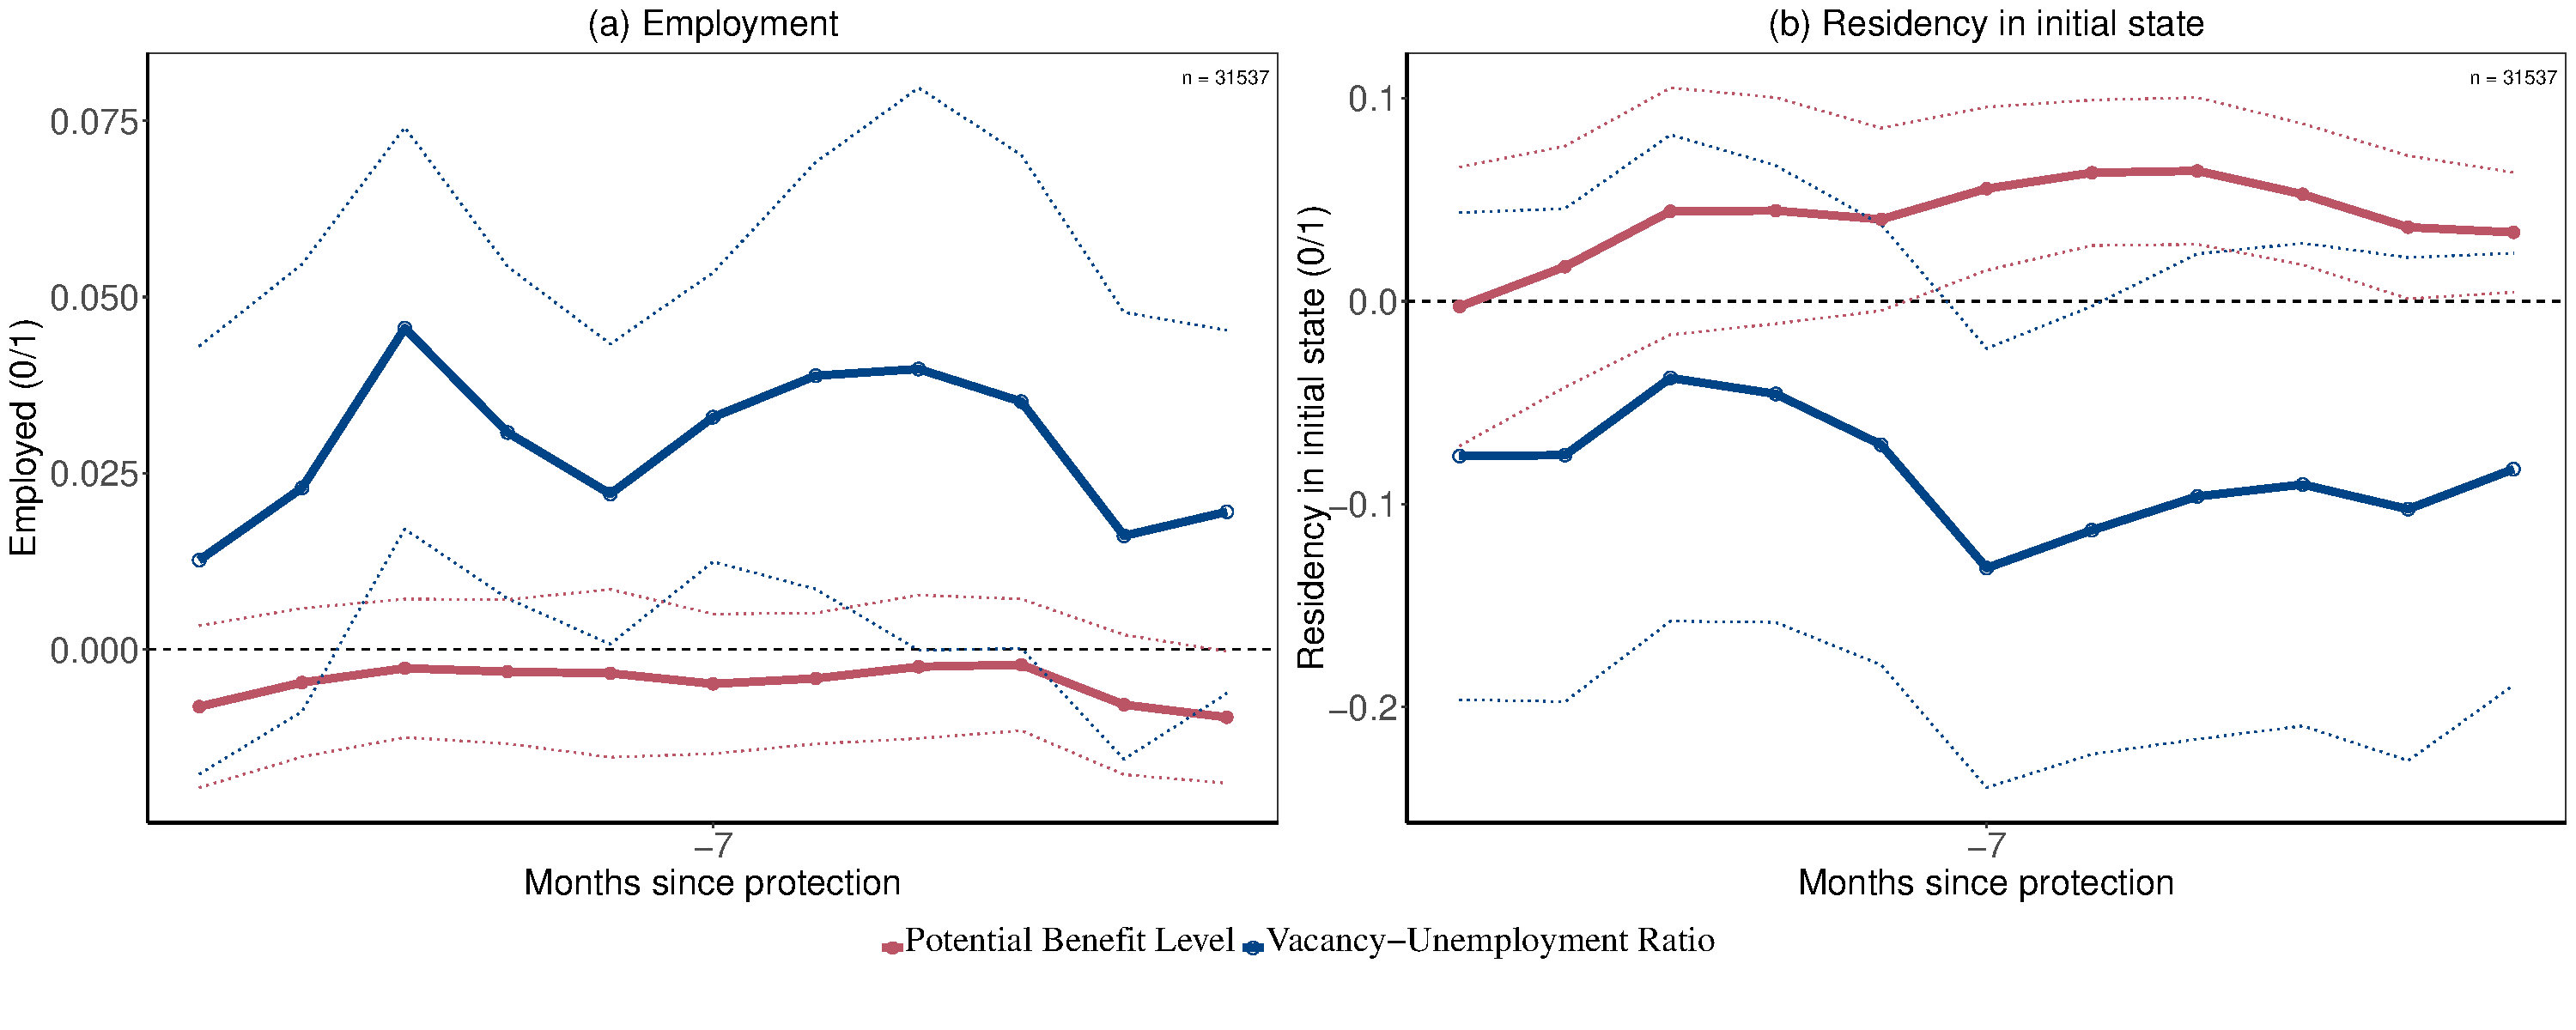
\includegraphics[scale=0.31]{figures/rob/fig_rob_labor_mobility_pre_trends_without_early_mover.pdf}
%     \end{center}
%     \fignote{Notes: The x-axis shows the months since protection was received. The y-axis displays the effect of a one-unit increase in either i) the vacancy-to-unemployment ratio or ii) the potential benefit level, measured in €1,000 (real 2015 values), on employment (left) and mobility (right). All regressions include a full set of arrival-group, year-month, and district-of-protection fixed effects. Additional control variables include age and age squared at immigration, gender, type of protection, family status at protection date, and country of origin. Standard errors are clustered at the district-year-of-protection level.}
% \end{figure}



% \begin{table}
%     \caption{Summary statistics excluding early movers}
%     \label{tab:summarystatistics_robustness}
%     \begin{threeparttable}
%         \begin{small}
%             \resizebox{\linewidth}{!}{%
%                 \begin{tabular}{lcccc}
%                     \expandableinput{figures/rob/descriptives_sample_without_early_movers.tex}
%                 \end{tabular}
%             }
%         \end{small}
%         \vspace{-1em}
%         \begin{tablenotes}
%             \parbox[t]{\textwidth}{%  % Set a strict width to the text width
%                 \fignote{Notes: The table reports means and standard deviations (in brackets) for continuous and binary variables. The number of observations and the percentage within groups are reported for categorical variables. Time-varying (outcome) variables are reported for the $12^th$ month after protection was received. The sample is restricted to refugees who received protection between January 2011 and August 2018, who were between 18 and 60 years old at the time of immigration and whose asylum process lasted longer than a day but less than three years, and where full data is available for 60 months after the date of protection. Family benefit eligibility is an indicator equal to one if children who are coinsured with this person or their partner are registered in Austria at the time of receiving protection. Duration asylum process is denoted in months and earnings are denoted in real 2015 euro.}
%             }
%         \end{tablenotes}
%     \end{threeparttable}
% \end{table}




%In Figure~\ref{fig:}, we further restrict the sample to asylum-seekers where we can confirm in the data that they were initially housed in one of the large reception centers. 
% initial placement
% standard errors

%\subsection{Event study analysis of individual reforms}

\FloatBarrier
\FloatBarrier
\section{\label{sec:discussion}Discussion}

Several additional considerations are important for interpreting our findings, particularly regarding the timing of our analysis, the temporal horizon of welfare benefits, and the impact of housing policies.

One insight from this paper is that regional differences in welfare generosity and labor market tightness at the time of protection—when refugees are particularly mobile—explain only a minor share of the observed variation in the propensity to move to Vienna (see Figure~\ref{fig:movermatrix}). It is beyond the scope of this paper to assess the relative importance of other factors, but we would like to mention some candidates. One potentially important aspect is variation in housing policy. Federal states adopt very different approaches to supporting refugees with housing after they receive protection, and some evidence suggests that these differences are correlated with outmigration to Vienna \citep{Dellinger2021Housing}.

There is also a clear east–west gradient: migration to Vienna is more common among refugees initially placed in eastern states, which are geographically closer to Vienna. While labor market conditions in the east are generally less favorable than in the west, our results suggest that these differences are not large enough to fully explain the observed migration patterns. Refugees in eastern regions likely face fewer barriers—both in terms of distance and cost, including through network effects—when considering a move to Vienna.

While a portion of our outcome window extends into the period affected by the COVID-19 pandemic, this does not compromise the internal validity of our results. By controlling for the exact timing of protection status in our empirical strategy, we account for all macro-level temporal shocks, including those related to the pandemic. It remains possible, however, that the pandemic may affect the external validity of our findings; outcomes might differ if the analysis were conducted in a different period or under different macroeconomic conditions. Importantly, it should be emphasized that the pandemic does not influence our estimates for the first 12 months after protection—the period where most of the observed effects occur—since our treatment window concludes in 2018. Thus, the core short-term results are entirely unaffected by pandemic-related developments.

The interpretation of our estimated effect sizes requires consideration of the variation in exposure to the policy change. Refugees living in private accommodation are directly affected by the reduction in benefit levels, as they experience immediate changes in disposable income. By contrast, individuals in organized accommodation receive almost all support in-kind. They are therefore not directly impacted by the reform, although the reduced benefit levels may still affect their decision-making if they consider transitioning to private accommodation. As we do not observe the type of accommodation at the individual level, our analysis necessarily mixes these types of exposure. Based on official statistics from the Grundversorgungsdatenbank,\footnote{See \url{https://www.migration-infografik.at/gvs-statistiken-2018}, retrieved July 30, 2025.} approximately 35\% of subsidiary-protected individuals outside Vienna reside in private accommodation. If we treat refugees in organized accommodation as fully unresponsive to benefit cuts---a strong assumption given the indirect channel just noted---our estimates for subsidiary-protected refugees scale by roughly a factor of three. This rescaling is therefore best read as a suggestive upper bound on the ATT for those directly exposed, since the in-kind group is unlikely to be entirely unaffected. For example, our standardized effect of a €300 reduction in benefit levels on the probability of staying in the assigned state for subsidiary-protected refugees is about -2.8 pp. at month 12; multiplying by three yields an ATT of -8.4 pp. The corresponding ATT for employment in month 12 is estimated at -4.5 pp. 

\subsection*{Policy Simulation}
\FloatBarrier

We also use our estimates to conduct back-of-the-envelope simulations of two hypothetical policies by predicting the outcomes for specified IPBL levels.

First, we assess the effect of setting benefit levels in all federal states equal to those in Vienna. Panel (a) of Table~\ref{tab:simulation} presents these results. This policy would slightly reduce employment rates after twelve months but has no effect after 60 months. It would lower the share of subsidiary-protected individuals who initially lived outside Vienna and later moved to Vienna by about two percentage points, while having almost no effect on Convention refugees, whose benefit levels were already more uniform across states.

Second, we assess the impact of aligning benefit levels for subsidiary-protected individuals with those of Convention refugees within each state. This policy — affecting only the subsidiary-protected — would reduce the employment rate by 1.1 pp. twelve months after protection and decrease the likelihood of moving to Vienna by slightly less than two percentage points (see Panel (b)).

\begin{table}
	\caption{Counterfactual results of various IPBL levels on employment and mobility}\label{tab:simulation}
	\begin{threeparttable}
		%\begin{small}
			%\begin{tabular}{lcccc}				
            %\begin{table}[ht]
\centering
%\begin{spacing}{1.5}
\label{tab:policy_simulation}
\renewcommand{\arraystretch}{1.2}
\begin{tabular}{l*{8}{>{\centering\arraybackslash}p{1cm}}}
%\begin{tabular}{lcccccccc}
\toprule
Protection Status & \multicolumn{4}{c}{Employed (\%)} 
& \multicolumn{4}{c}{Moved to Vienna (\%)} \\
  & \multicolumn{2}{c}{12 months} 
  & \multicolumn{2}{c}{60 months} 
  & \multicolumn{2}{c}{12 months}
  & \multicolumn{2}{c}{60 months} \\
\cmidrule(lr){2-3} \cmidrule(lr){4-5} \cmidrule(lr){6-7} \cmidrule(lr){8-9}
& Base & CF & Base & CF & Base & CF & Base & CF \\
\midrule
\multicolumn{9}{c}{\textit{a. IPBL in all states to Viennese levels}} \\
Overall & 13.9 & 13.4 & 45.7 & 45.7 & 26.6 & 25.9 & 33.7 & 32.9 \\
Convention refugees & 11.7 & 11.6 & 43.6 & 43.6 & 22.8 & 22.5 & 30.7 & 30.5 \\
Subsidiary-protected & 20.4 & 19.1 & 52.1 & 52.1 & 37.5 & 35.4 & 42.0 & 39.7 \\
\\
\multicolumn{9}{c}{\textit{b. IPBL for subsidiary-protected set to the levels for Convention refugees in the state}} \\
Subsidiary-protected & 20.4 & 19.3 & 52.1 & 52.1 & 37.5 & 35.8 & 42.0 & 40.1 \\
\bottomrule
\end{tabular}


% \begin{tabular}{lcccccccc}
% \toprule
% Protection Status 
%     & \multicolumn{4}{c}{Employed (\%)} 
%     & \multicolumn{4}{c}{Moved to Vienna (\%)} \\
%   & \multicolumn{2}{c}{12 months} 
%   & \multicolumn{2}{c}{60 months} 
%   & \multicolumn{2}{c}{12 months} 
%   & \multicolumn{2}{c}{60 months}  \\
% \cmidrule(lr){2-3} \cmidrule(lr){4-5} \cmidrule(lr){6-7} \cmidrule(lr){8-9}
% & Base & CF & Base & CF & Base & CF & Base & CF \\
% \midrule
% \multicolumn{9}{c}{\textit{a. IPBL in all states to Viennese levels}} \\
% Overall & 0.139 & 0.134 & 0.457 & 0.457 & 0.266 & 0.259 & 0.337 & 0.329\\
% Convention refugees & 0.117 & 0.116 & 0.436 & 0.436 & 0.228 & 0.225 & 0.307 & 0.305\\
% Subsidiary-protected & 0.204 & 0.191 & 0.521 & 0.521 & 0.375 & 0.354 & 0.420 & 0.397\\
% \\
% \multicolumn{9}{c}{\textit{b. IPBL for subsidiary-protected set to the levels for Conventions refugees in the state}} \\
% Subsidiary-protected & 0.204 & 0.193 & 0.521 & 0.521 & 0.375 & 0.358 & 0.420 & 0.401\\
% \end{tabular}
% %\end{table}

% %%prozent + 1 decimal, mehr abstand
			%\end{tabular}
		%\end{small}
		\begin{tablenotes} 
			\begin{footnotesize}
				\begin{spacing}{1}
					\textit{Notes:} The table shows counterfactual predictions for employment and residency in Vienna under alternative IPBL scenarios. In Scenario a, we set the IPBL levels for all protection types in each state to match the corresponding Vienna levels of each year. Column ``Base'' shows the baseline predictions for employment and staying in Vienna from our main specification. Column ``CF'' shows the counterfactual shares under the policy change. 
                    In Scenario b, we adjust the IPBL levels for subsidiary-protected refugees to equal those of Convention refugees within the same state and year. The sample includes only refugees who received protection in 2017.  
				\end{spacing}
			\end{footnotesize}
		\end{tablenotes}
	\end{threeparttable}
\end{table}

\FloatBarrier
\FloatBarrier
%%%%%%%%%%%%%%%%%%%%%%%%%%%%%%%%%%%%%%%%%%%%%%%%%%%%%%%%%%%%%%%%%%%%%%%%%%%%%%%%%%%%%%%%%%%%%%%%%%%%%%%%%%%%
%%%%%%%%%%%%%%%%%%%%%%%%%%%%%%%%%% CONCLUSION   %%%%%%%%%%%%%%%%%%%%%%%%%%%%%%%%%%%%%%5%%%%%%%%%%%%%%%%%%%%%
%%%%%%%%%%%%%%%%%%%%%%%%%%%%%%%%%%%%%%%%%%%%%%%%%%%%%%%%%%%%%%%%%%%%%%%%%%%%%%%%%%%%%%%%%%%%%%%%%%%%%%%%%%%%

%Notably, the data coverage is more extensive for subsidiary-protected  individuals compared to Geneva Convention (GC) refugees. For the years with most asylum-seekers arriving in Austria, the coverage is especially commendable, reaching 67\% for GC refugees and 96\% for subsidiary-protected  individuals in the year 2015. The arrivals years with the highest number of asylum applications and the highest shares of coverage in our data, are also the main arrival years for our analysis sample. This reduces the possible selection bias. 


\FloatBarrier
\section{\label{sec:conclusion}Conclusion}

This study examines the interplay between local labor market conditions and welfare generosity on the labor market integration and internal mobility of refugees. Utilizing detailed register data, we analyze how refugees respond to the conditions they encounter when their choice set expands upon receiving protection.
Many initially dispersed refugees relocate as soon as they are allowed to do so. Their decision to relocate is influenced by both labor demand and welfare generosity at their initial placement location.

We show that labor demand, particularly in occupations with low entry barriers, immediately and significantly increases labor force participation among men. However, this effect fades after 2.5 years. In turn, tighter labor markets raise the likelihood of staying in the assigned state permanently.
Higher benefit levels decrease the likelihood of relocation but temporarily lower men’s employment levels and more persistently affect women’s employment, although the effect sizes are relatively small.

Lastly, when examining the interaction between labor market tightness and benefit levels, we find that changes in welfare benefits have a stronger effect on employment rates when local labor markets are tight and are negligible otherwise, consistent with similar findings for Denmark \citep{dustmann2024}.

By examining both relocation and employment, we show that tighter local labor markets encourage refugees to remain in their state and secure employment rather than relocate to another state without employment. Higher benefit levels have a minor negative effect on the probability of securing employment in the initial state but increase the likelihood of remaining without employment instead of moving and being unemployed elsewhere. Overall, our findings suggest that mobility responses to initial labor-market conditions and welfare benefit levels are more reflective of short-term needs than long-term optimization regarding labor market prospects, resembling the findings of work-first policies \citep{arendt_labor_2022, arendt_trade-offs_2023}.

From a policy perspective, our findings show that supporting refugees in finding employment at the moment of, or even before, receiving protection may prevent their migration to other regions. Additionally, they highlight the importance of considering the labor market conditions in the districts to which refugees are allocated. At the same time, changes in benefits will only affect labor market integration in strong labor markets. Thus, welfare reforms aimed at incentivizing employment among refugees will be effective only in regions with strong labor markets.

\begin{comment}
Our data revealed a positive effect of the $IVUR$ and refugee employment. A shift of two quartiles in the $IVUR$ leads to a 4.2 percentage point increase in the likelihood of employment by the 12th month, a substantial 37\% rise relative to the baseline employment rate in the same period. On the contrary, a similar two quartile shift in the $IPBL$ results in a 2.3 percentage point decrease in the employment probability, a 20.3\% reduction from the baseline.

Monthly Real Earnings: An upward shift in the $IVUR$ from the first to the third quartile corresponds to an increase of €84.6 in monthly real earnings, a notable 41\% rise relative to the mean in month 12. In contrast, a similar shift in the $IPBL$ leads to a reduction of €50.01 in earnings, a 24\% decline from the month 12 mean. Furthermore, every increase of €100 in potential benefits results in an €11 reduction in monthly real earnings.
In simpler terms, regions with more job openings relative to the number of unemployed individuals offer better employment opportunities for refugees. This observation underscores the pivotal role of immediate job availability in early labor market integration. Conversely, higher potential benefit levels tend to discourage refugees from entering the labor market promptly. While these benefits are crucial for the well-being of refugees, they might also serve as a deterrent to seeking employment. This highlights the trade-offs refugees face between labor market participation and accessing socio-economic support. However, our analysis does not conclusively determine whether rapid integration into the labor market might compel refugees to accept jobs that do not align with their qualification profiles, potentially impeding their long-term trajectories.

Interestingly, the effects of both the $IVUR$ and $IPBL$ on economic outcomes were found to be short-lived, losing significance within 24 months after refugees gained labor market access. This suggests that while initial conditions play a role, their impact diminishes over time.

Expanding on mobility outcomes, alterations in the $IPBL$ and $IVUR$ significantly influenced the likelihood of refugees staying in their initially assigned states. Notably, a 0.456 change in the $IPBL$ resulted in a 4.2 percentage point increase and a 0.211 change in the $IVUR$ resulted in a 4.1 percentage point increase, with both effects being comparatively persistent over time. Furthermore, increased potential benefits reduced the likelihood of refugees relocating to Vienna, signaling the role of benefits in influencing mobility patterns.
When observing social support outcomes, there was no significant effect from either the $IVUR$ or $IPBL$ on the utilization of public employment service (PES) services. However, a shift in the $IVUR$ from the first to the third quartile reduced the likelihood of refugees receiving welfare benefits by 4.9 percentage points, reinforcing the inverse relationship between employment and reliance on welfare benefits.
From a policy perspective, our findings highlight the importance of providing adequate job opportunities in regions with significant refugee placements. At the same time, it's vital to structure benefits in a way that supports refugees without discouraging labor market participation. Additionally, ensuring robust social support structures is an important aspect when it comes to social integration, potentially reducing the need to relocate to other parts of a country due to financial restraints. 
In conclusion, our research sheds light on the multifaceted aspects of refugee labor market integration in the Austrian context. The balance between job opportunities, socio-economic benefits, mobility, and social support, along with the time-bound nature of their effects, offers important insights for policymakers and stakeholders involved in refugee integration.
\end{comment}



%




%%%%%%%%%%%%%%%%%%%%%%%%%%%%%%%%%%%%%%%%%%%%%%%%%%%%%%%%%%%%%%%%%%%%%%%%%%%%%%%%%%%%%%%%%%%%%%%%%%%%%%%%%%%%
%%%%%%%%%%%%%%%%%%%%%%%%%%%%%%%%%% THEORY  %%%%%%%%%%%%%%%%%%%%%%%%%%%%%%%%%%%%%%%%%%%%%%%%%%%%%%%%%%%%%%%%%
%%%%%%%%%%%%%%%%%%%%%%%%%%%%%%%%%%%%%%%%%%%%%%%%%%%%%%%%%%%%%%%%%%%%%%%%%%%%%%%%%%%%%%%%%%%%%%%%%%%%%%%%%%%%

% \section{Conceptual Framework} \label{sec:framework}
% \textbf{ADD SOME THEORY ON HOW INITIAL LABOR MARKET CONDITIONS AFFECT REFUGEE INTEGRATION. FOR NOW IT COULD JUST BE A LITERATURE OVERVIEW.}










%%%%%%%%%%%%%%%%%%%%%%%%%%%%%%%%%%%%%%%%%%%%%%%%%%%%%%%%%%%%%%%%%%%%%%%%%%%%%%%%%%%%%%%%%%%%%%%
% REFERENCES
%%%%%%%%%%%%%%%%%%%%%%%%%%%%%%%%%%%%%%%%%%%%%%%%%%%%%%%%%%%%%%%%%%%%%%%%%%%%%%%%%%%%%%%%%%%%%%%
\newpage

\bibliographystyle{ecta}
\bibliography{bib_andreas}{}

%%%%%%%%%%%%%%%%%%%%%%%%%%%%%%%%%%%%%%%%%%%%%%%%%%%%%%%%%%%%%%%%%%%%%%%%%%%%%%%%%%%%%%%%%%%%%%%
% Appendix
%%%%%%%%%%%%%%%%%%%%%%%%%%%%%%%%%%%%%%%%%%%%%%%%%%%%%%%%%%%%%%%%%%%%%%%%%%%%%%%%%%%%%%%%%%%%%%%
\newpage
\begin{appendix}
    \part*{Appendix}
    \pagenumbering{roman}
    \setcounter{page}{1} 
    \setcounter{footnote}{0}
    
    \renewcommand\theequation{\Alph{section}.\arabic{equation}}
    \setcounter{figure}{0}  \renewcommand{\thefigure}{\Alph{section}.\arabic{figure}} 
    \setcounter{table}{0} \renewcommand{\thetable}{\Alph{section}.\arabic{table}}

    %%%%%%%%%%%%%%%%%%%%%%%%%%%%%%%%%%%%%%%%%%%%%%%%%%%%%%%%%%%%%%%%%%%%%%
% Appendix: Tables and Figures
%%%%%%%%%%%%%%%%%%%%%%%%%%%%%%%%%%%%%%%%%%%%%%%%%%%%%%%%%%%%%%%%%%%%%%%%%%%%%%%%%%%%%%%%%%%%%%%

%Appendix to Wett , V., Gallegos Torres, K. and Steinmayr, A. (2023). Opportunities or Benefits: Local Conditions and Refugee Labor Market Integration %In: \emph{Journal}. 


%\section{Unused Figures Appendix}

\FloatBarrier


% \begin{figure}
%     \caption{Robustness: Different Standard Errors and Wild Cluster Bootstrap}
%     \label{fig:errors}
%     \begin{center}
%     \vspace{-0.5 cm}
%     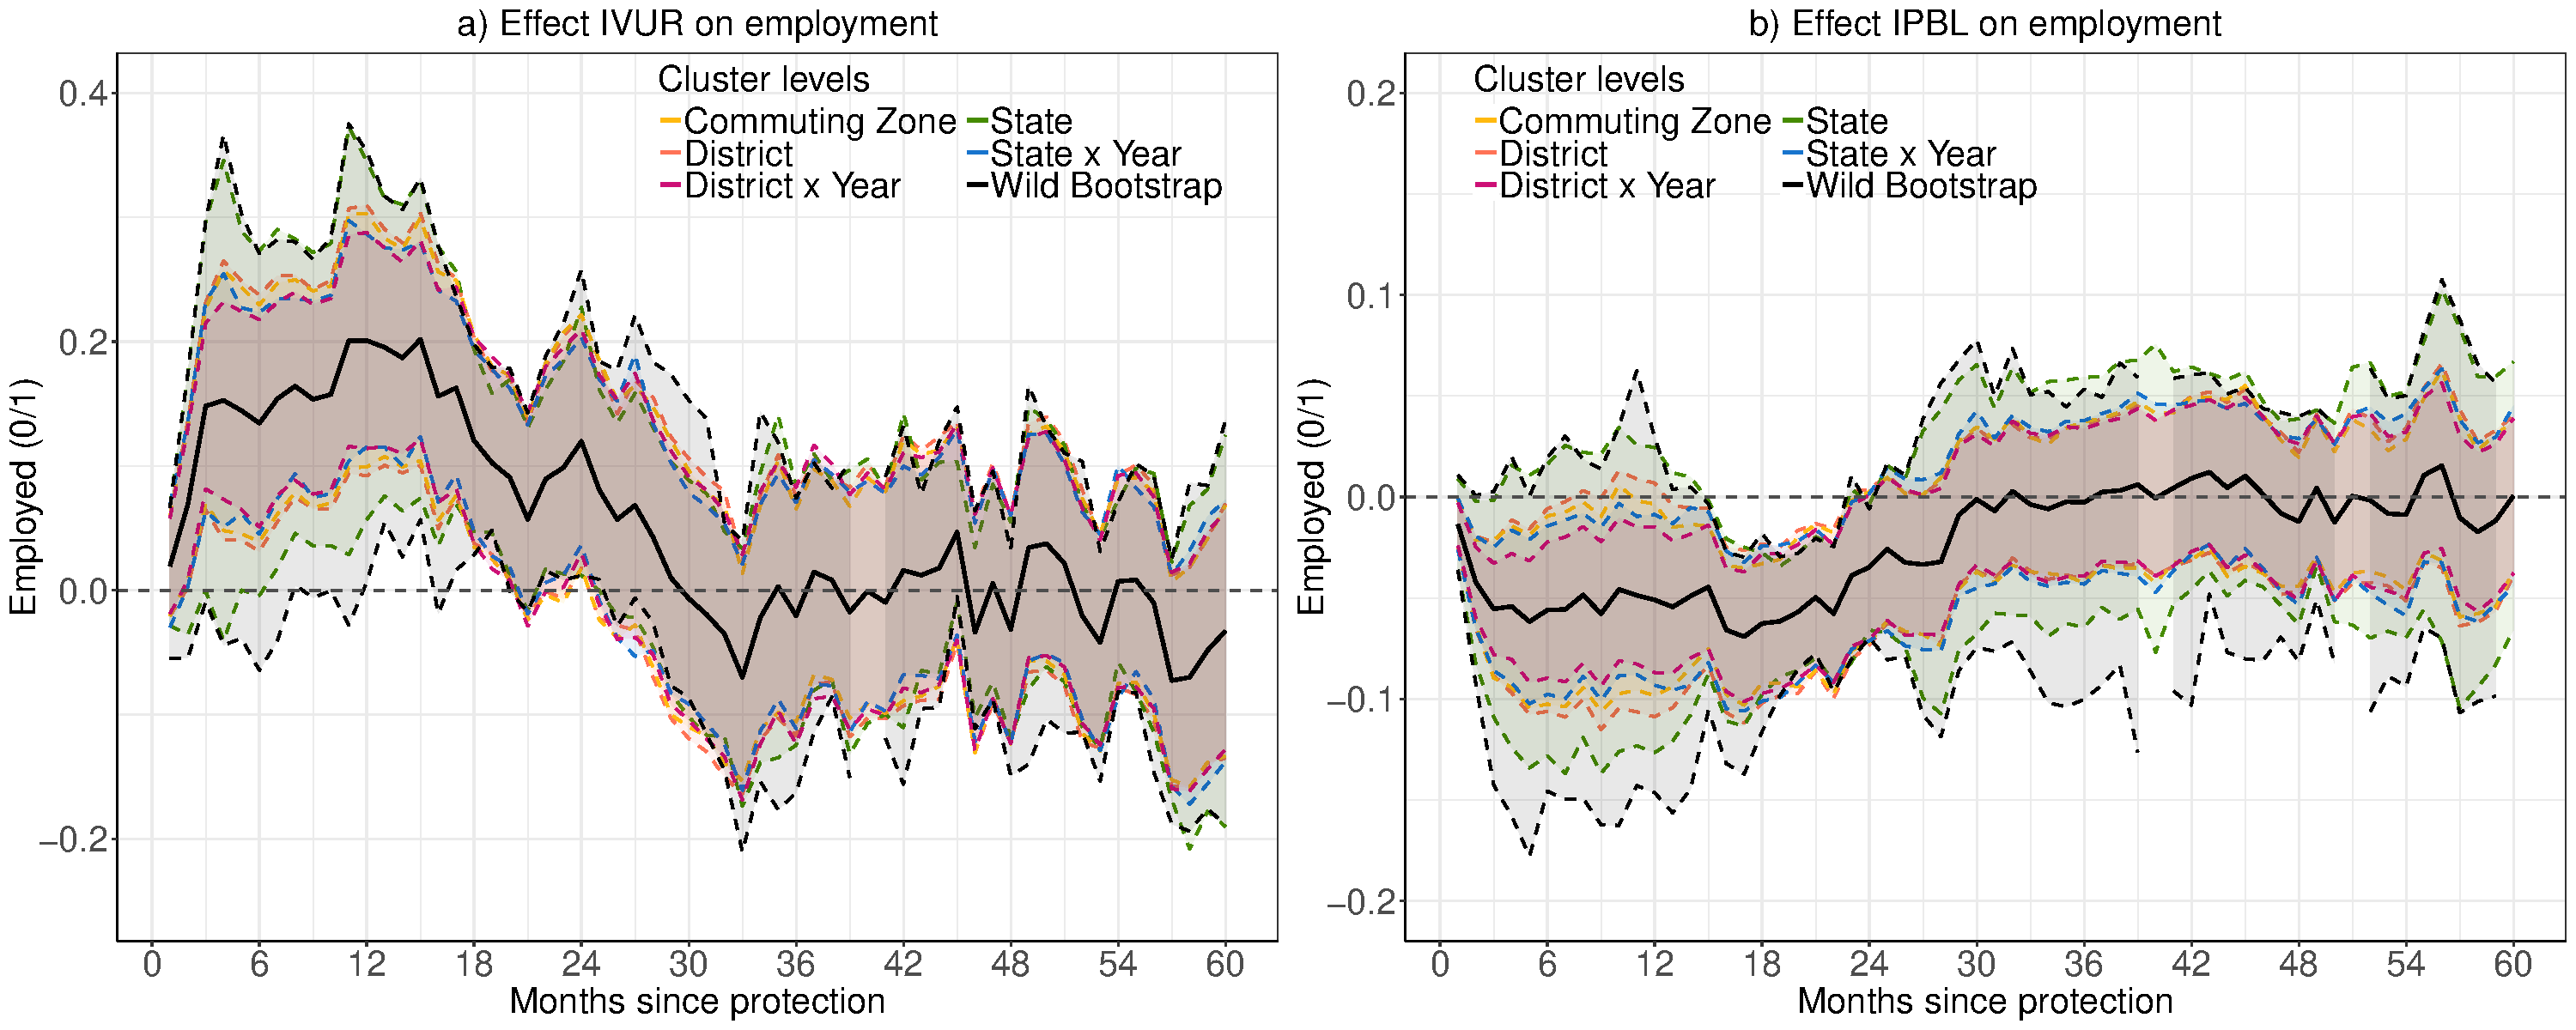
\includegraphics[scale=0.31]{figures/rob/different_standard_errors.pdf}
%     \end{center}
%     \vspace{-0.5 cm}
%     \fignote{\footnotesize \textit{Notes:} Comparison of the estimated effects of the vacancy-to-unemployment ratio (left) and the potential benefit level (right) on employment. Each plot shows the point estimates and confidence intervals using standard errors clustered at alternative aggregation levels (district, state, commuting zone, state~$\times$~year, district~$\times$~year), as well as wild cluster bootstrap intervals. Each dotted pair of confidence intervals corresponds to a different clustering level for the calculation of standard errors. Black lines indicate confidence intervals from wild cluster bootstrap procedures using Rademacher weights for the IVUR and Webb weights for the IPBL.}
% \end{figure}





% \begin{figure}
%     \caption{Robustness: Internal Mobility Patterns by Initial Location Type}
%     \label{fig:errors}
%     \begin{center}
%     \vspace{-0.5 cm}
%     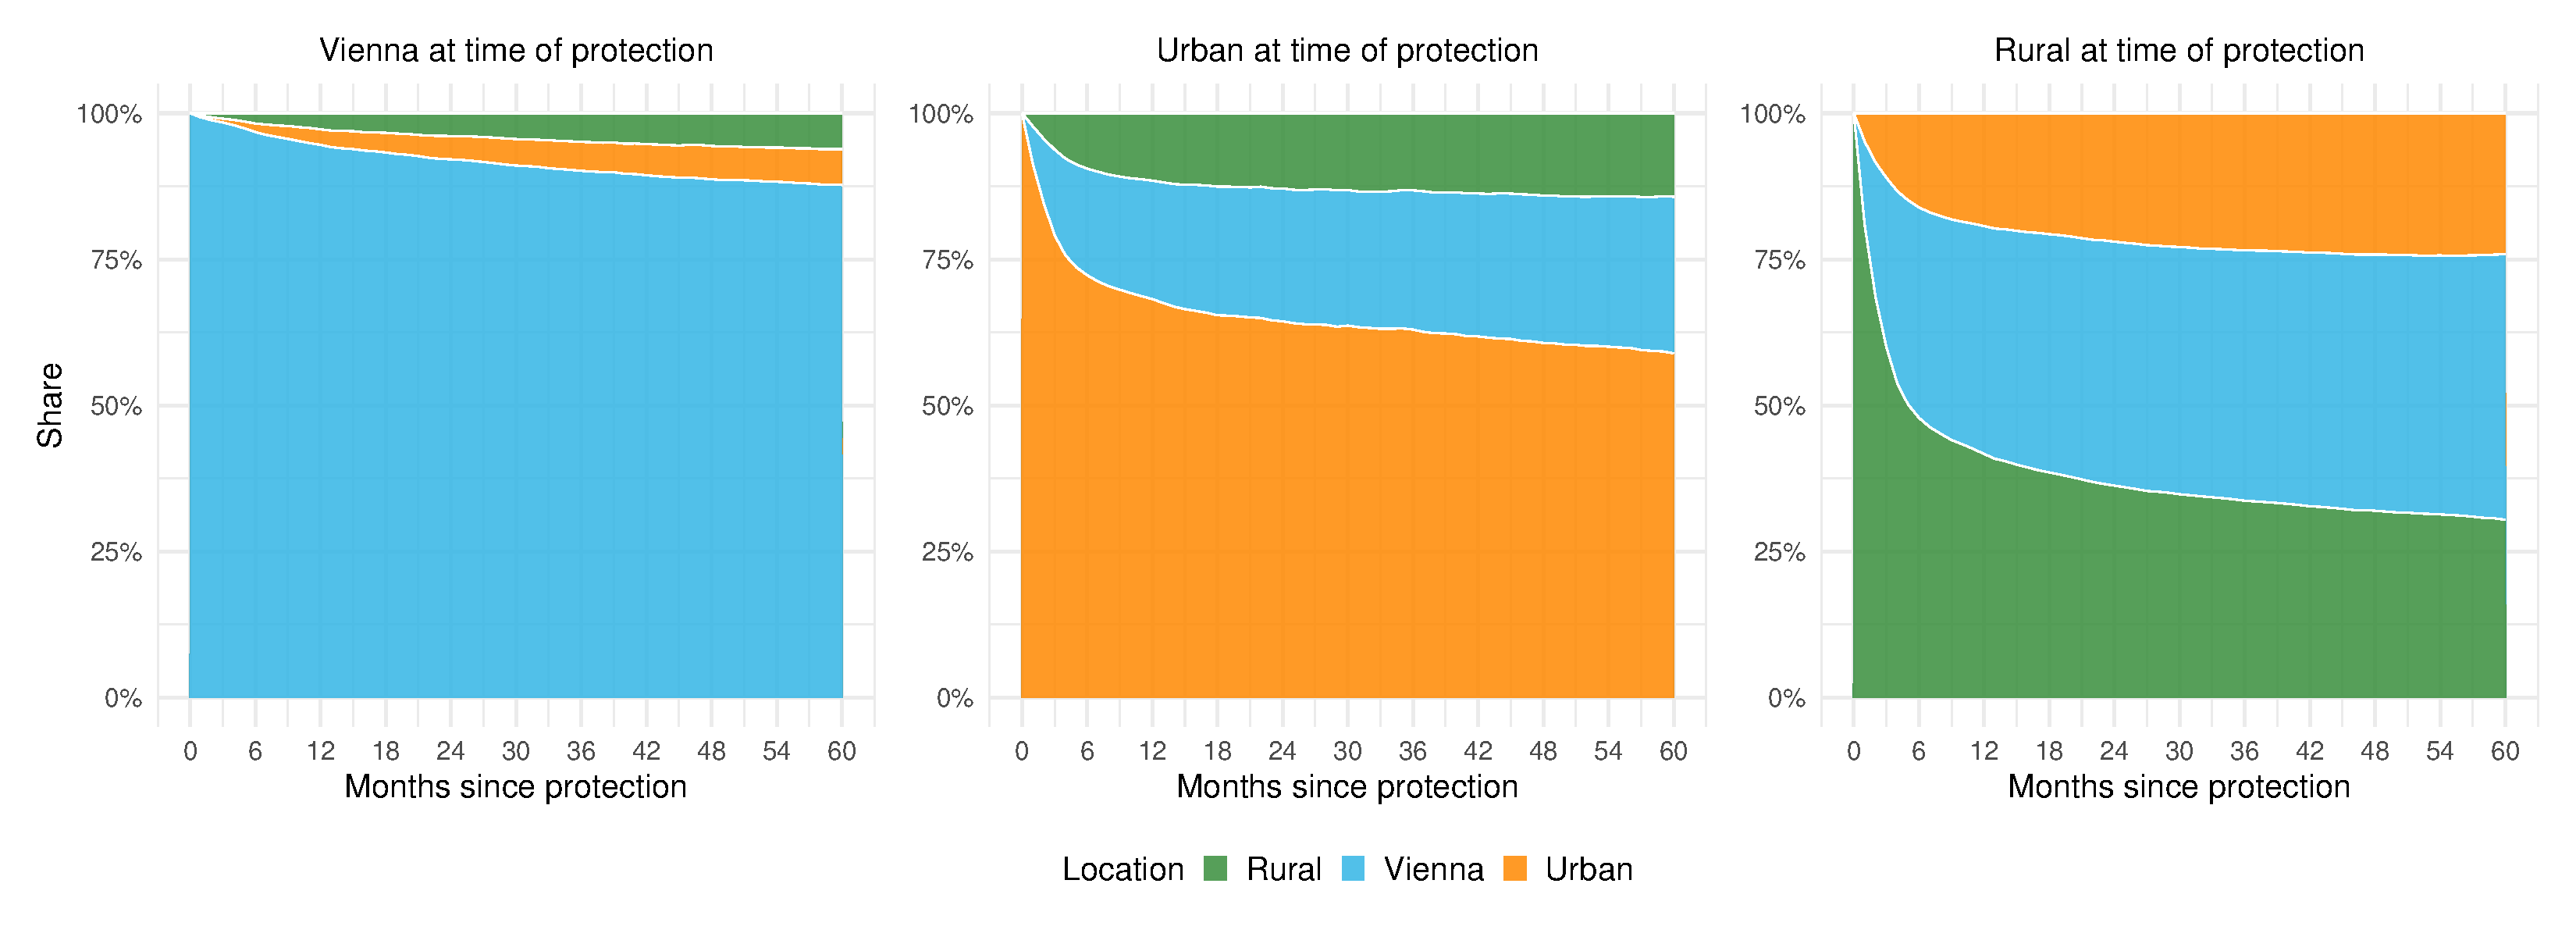
\includegraphics[scale=0.29]{figures/rob/fig_urban_rural.pdf}
%     \end{center}
%     \vspace{-0.5 cm}
%     \fignote{\footnotesize \textit{Notes:} The figure shows the share of individuals in each municipality type (Vienna, urban, rural) over time, conditional on their baseline location at the time of protection. Municipalities are defined as urban if they have a population greater than 20,000 inhabitants in 2011 (excluding Vienna) and rural otherwise. Stacked area charts are shown separately for each group.}
% \end{figure}


% \begin{figure}
%     \caption{Robustness: Leave-One-State-Out Analysis}
%     \label{fig:errors}
%     \begin{center}
%     \vspace{-0.5 cm}
%     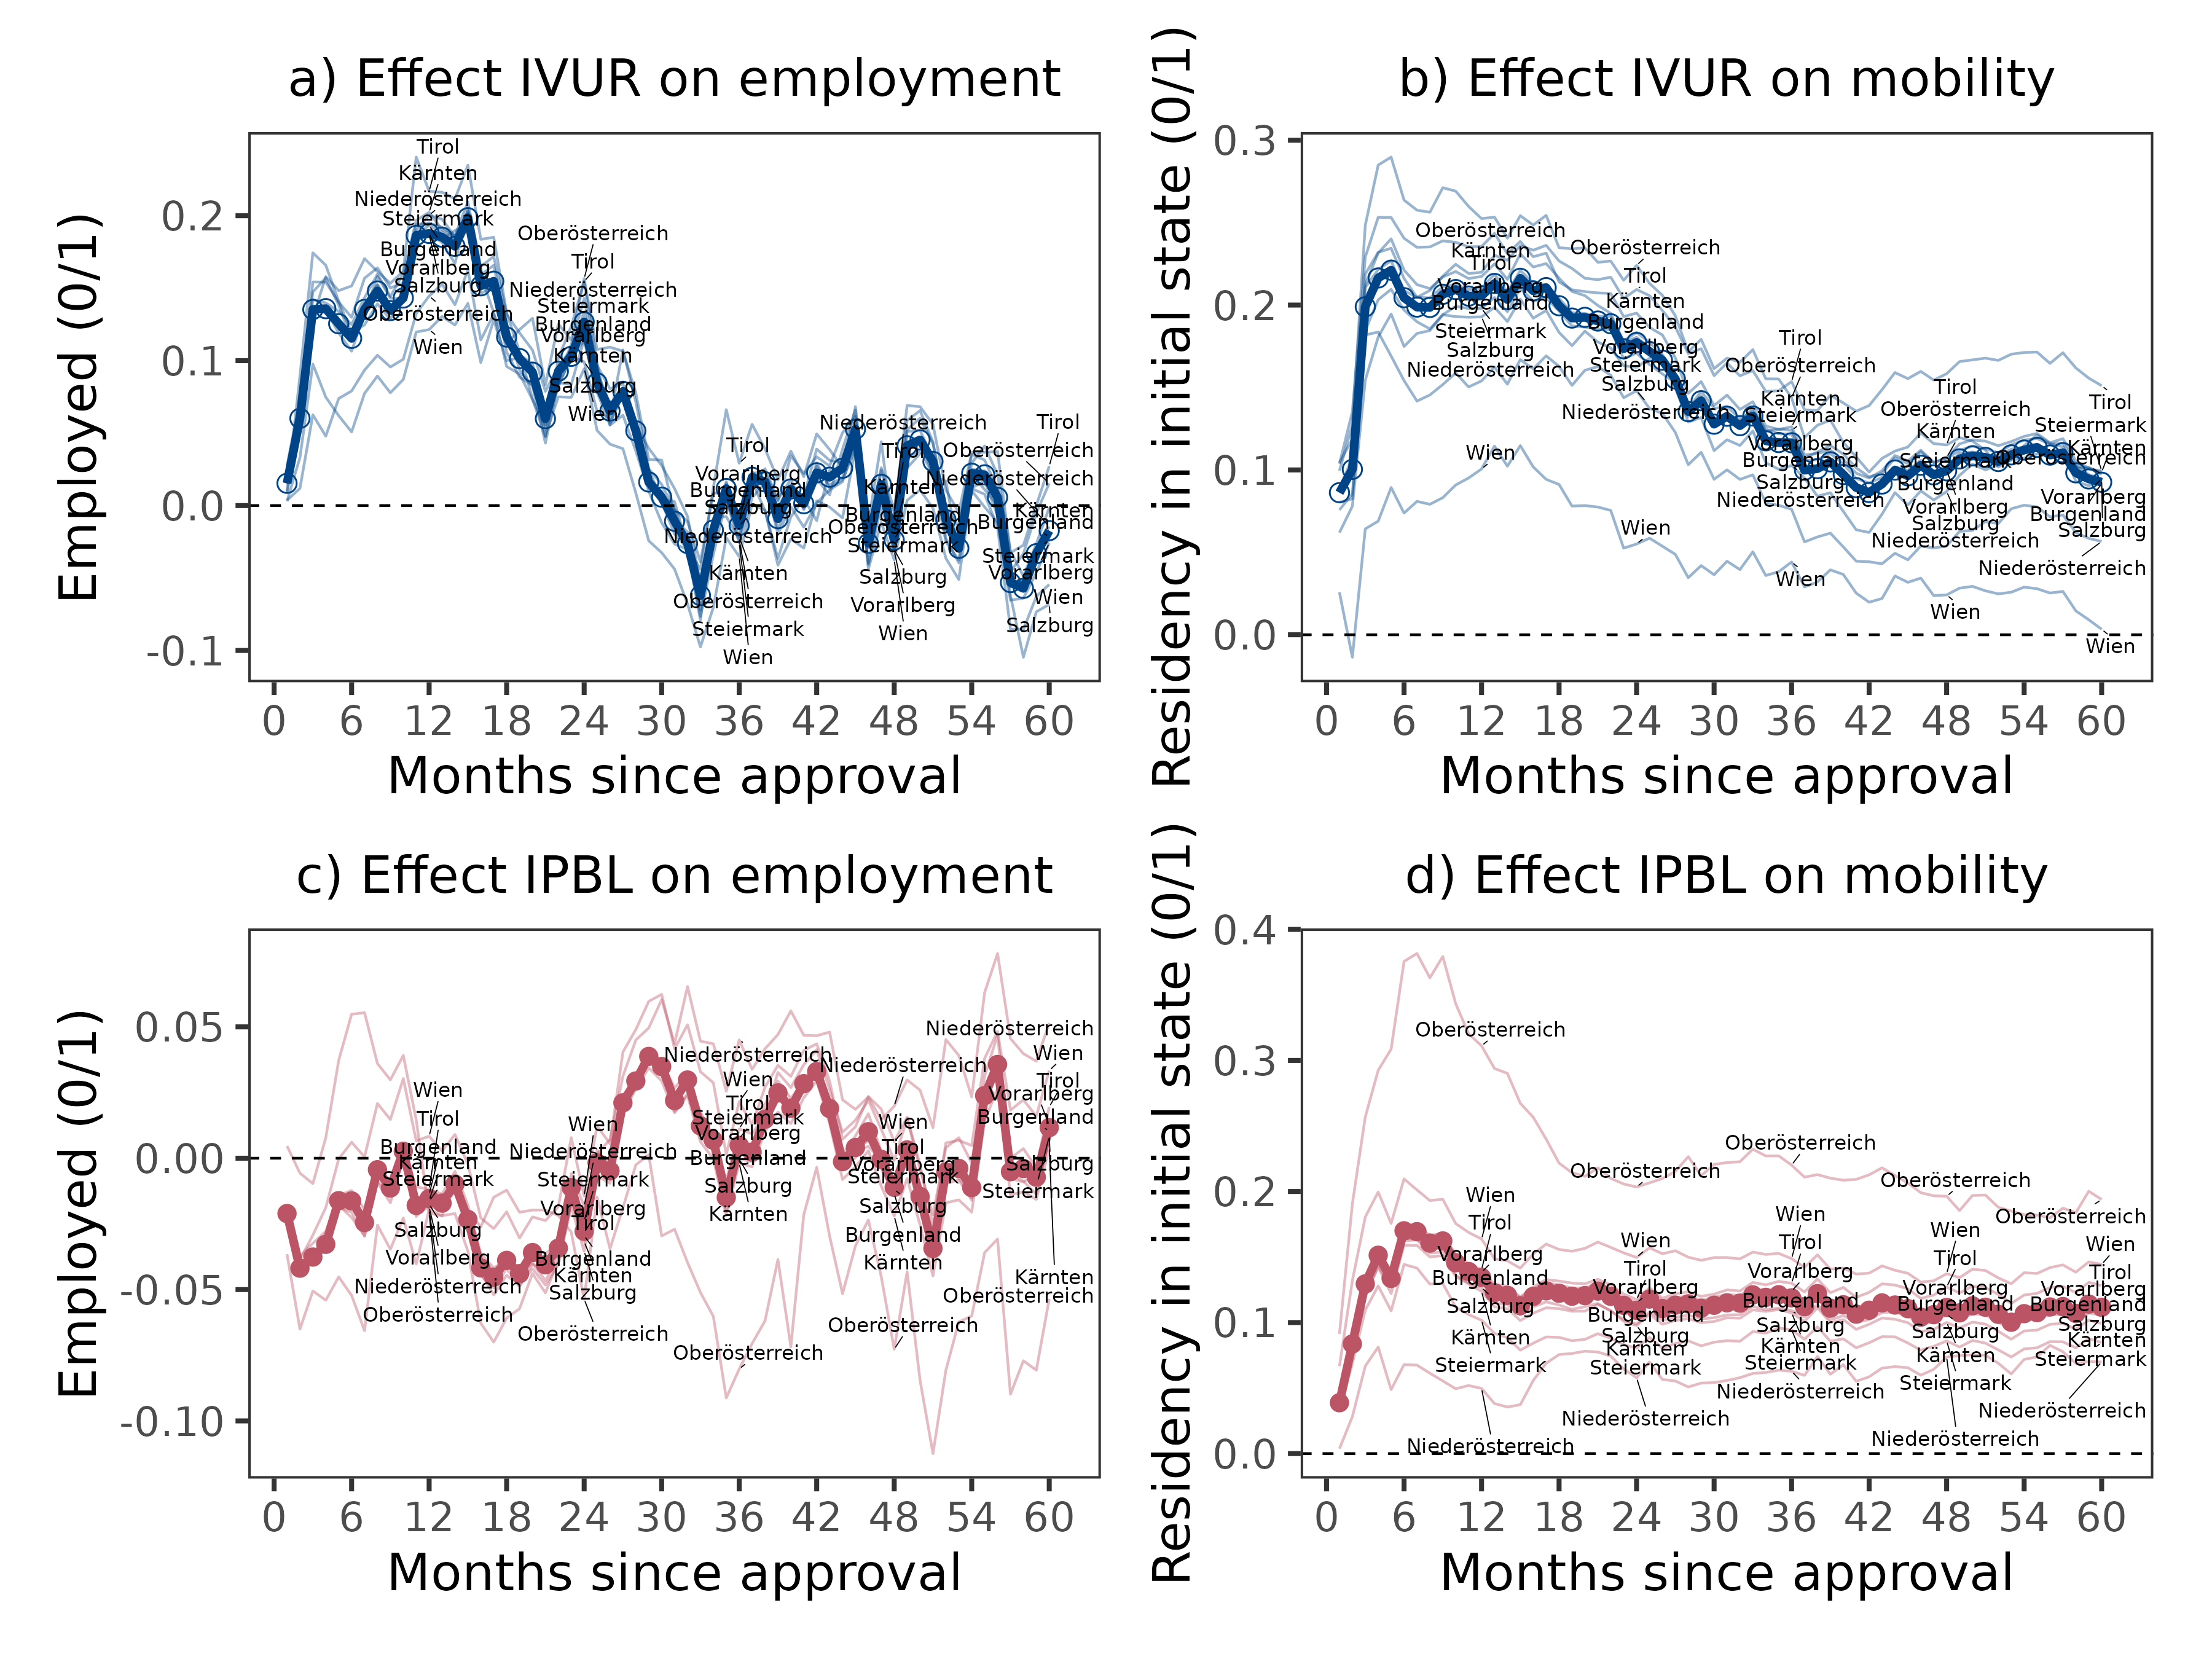
\includegraphics[scale=0.50]{figures/rob/leavestate_fourplots_withlabels.png}
%     \end{center}
%     \vspace{-0.5 cm}
%     \fignote{\footnotesize \textit{Notes:} The thick lines correspond to the main results from figures \ref{fig:mobility_results} (a) and \ref{fig:empl_reloc} (a). Each thin line corresponds to re-estimating the main model after excluding one state at time of protection group from the sample.}
% \end{figure}





\FloatBarrier




\section{Additional Tables and Figures}
\FloatBarrier


\subsection{Welfare benefit levels for refugees (families) by federal state} \label{family}


\begin{figure}
    \caption{Welfare benefit levels for refugees (families) by federal state}
    \label{fig:ipbl_family}
    \begin{center}
    \vspace{-0.8 cm}
    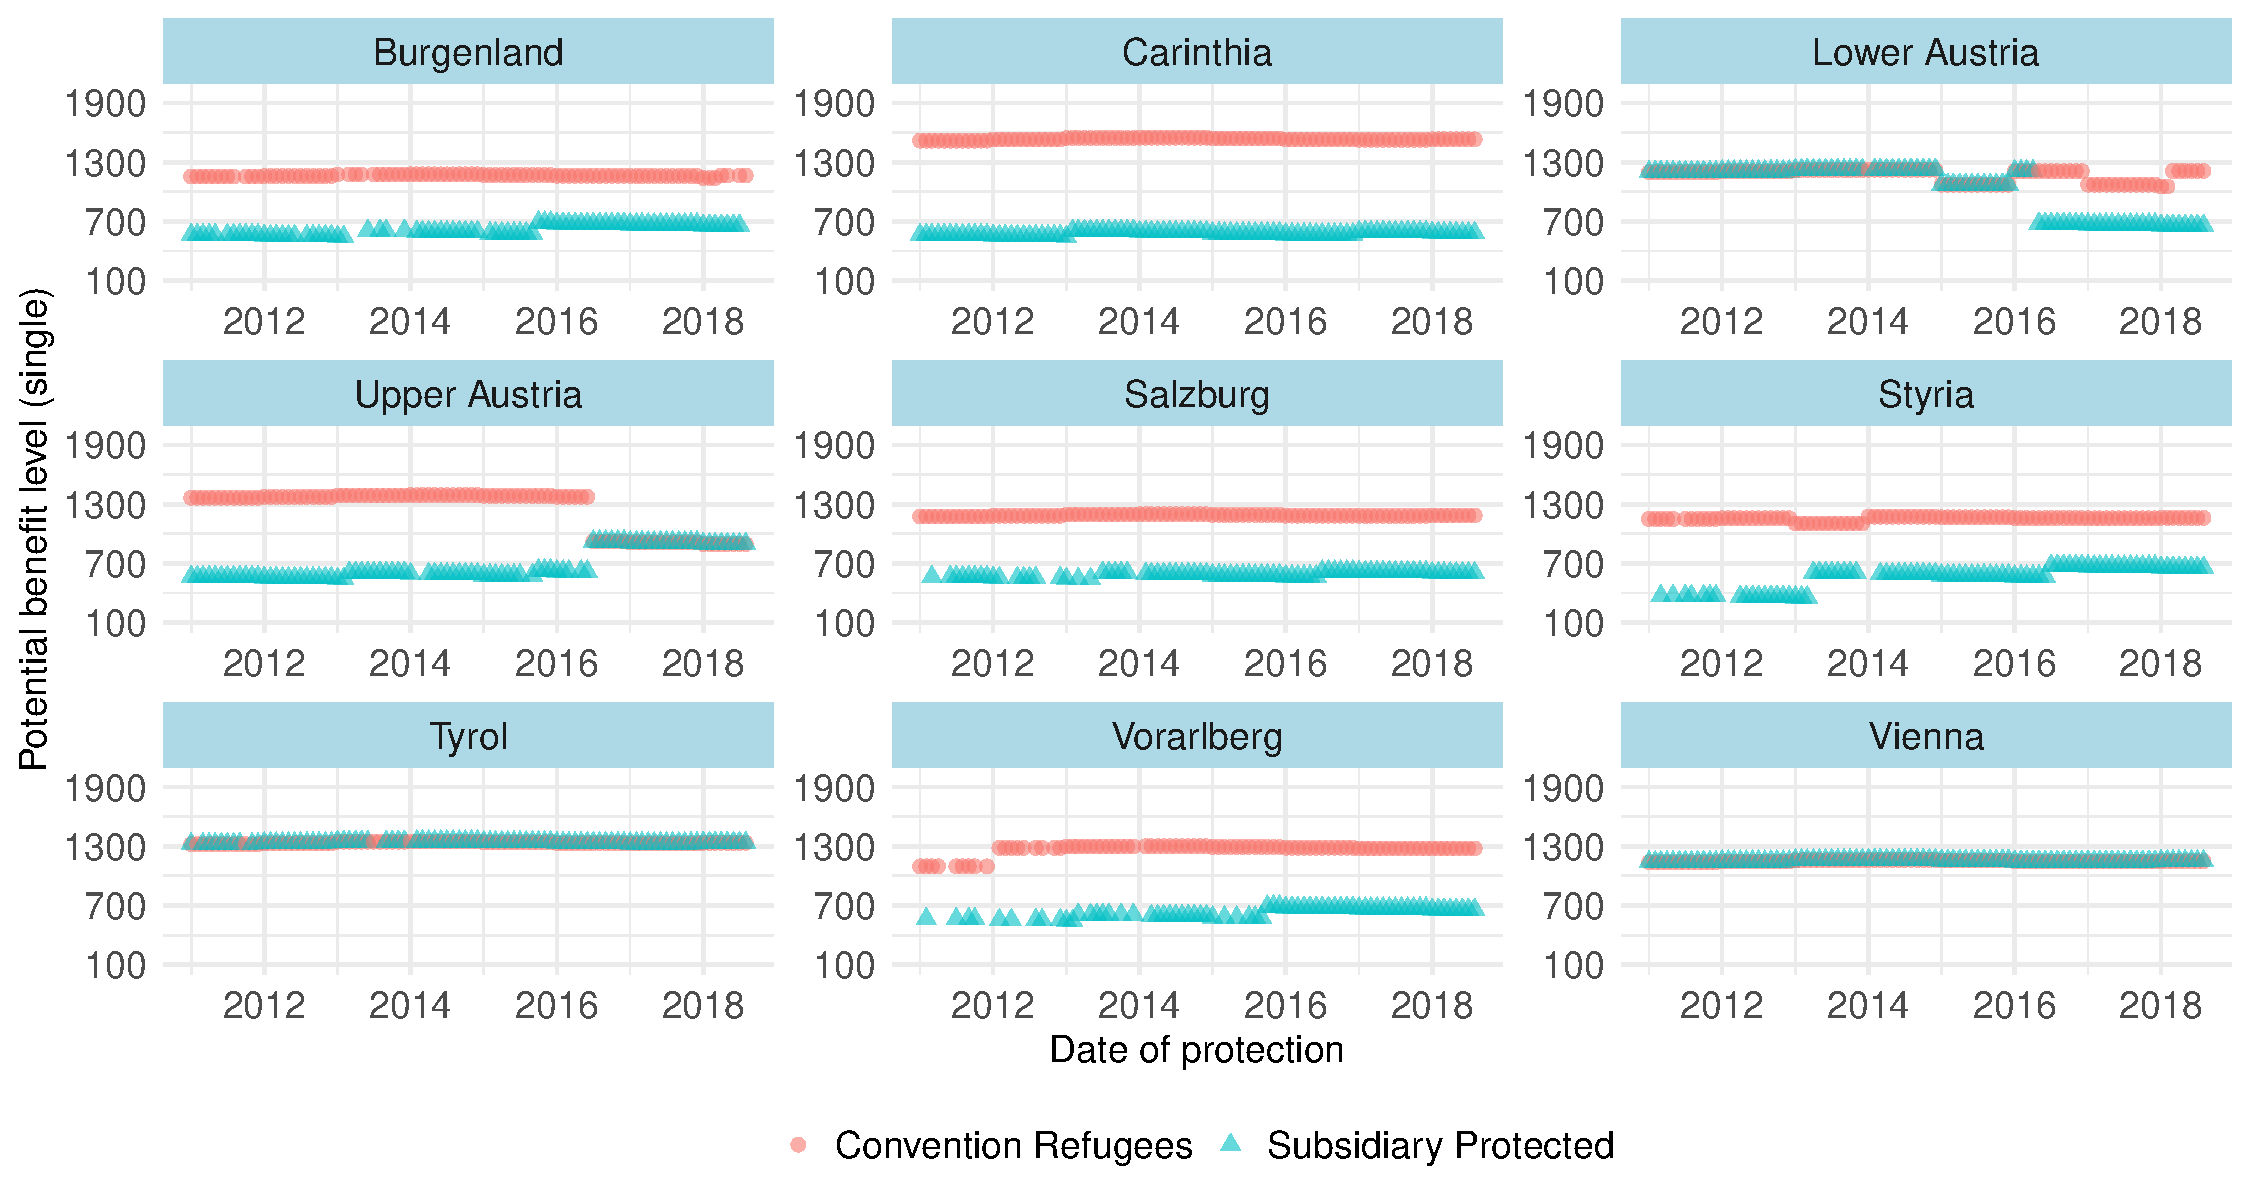
\includegraphics[scale=0.4]{figures/fig_ipbl_family.pdf}
    \end{center}
    \vspace{-0.7cm}
    \justify 
 		{\footnotesize 
 			\textit{Notes:}
    %\fignote{Notes: 
    The figure shows the amount of monthly benefits in euros (excluding housing benefits) for families consisting of two adults and two children by federal state and type of protection.}
\end{figure}


\FloatBarrier
\subsection{Effect on likelihood to remain in Austria} \label{no_insurance}

To test for potential sample selection, we evaluate whether $IVUR$ and $IPBL$ affect the likelihood of remaining in Austria, indicated by maintaining an active social insurance spell. Figure~\ref{fig:data_gaps} illustrates the impact of a one-unit rise in $IVUR$ and a €1,000 increase in $IPBL$ over time. It displays the month-specific coefficients $\beta_{1,t}$ and $\beta_{2,t}$ from our main model (Equation \ref{eq:main}) for the initial 60 months post-protection.

$IVUR$ and $IPBL$ have no effect on the likelihood of remaining insured in Austria. In essence, higher labor demand or increased welfare benefits do not influence the decision to stay in or leave Austria. While interesting in itself, this observation enables us to proceed with our study using a smaller cohort of 39,694 individuals who are still present in Austria after five years, since the selection process appears not to be influenced by our variables of interest.

\begin{figure}
    \caption{Effect of $IVUR$ and $IPBL$ on the probability of remaining insured in Austria}
    \label{fig:data_gaps}
    \begin{center}
    \vspace{-0.8 cm}
    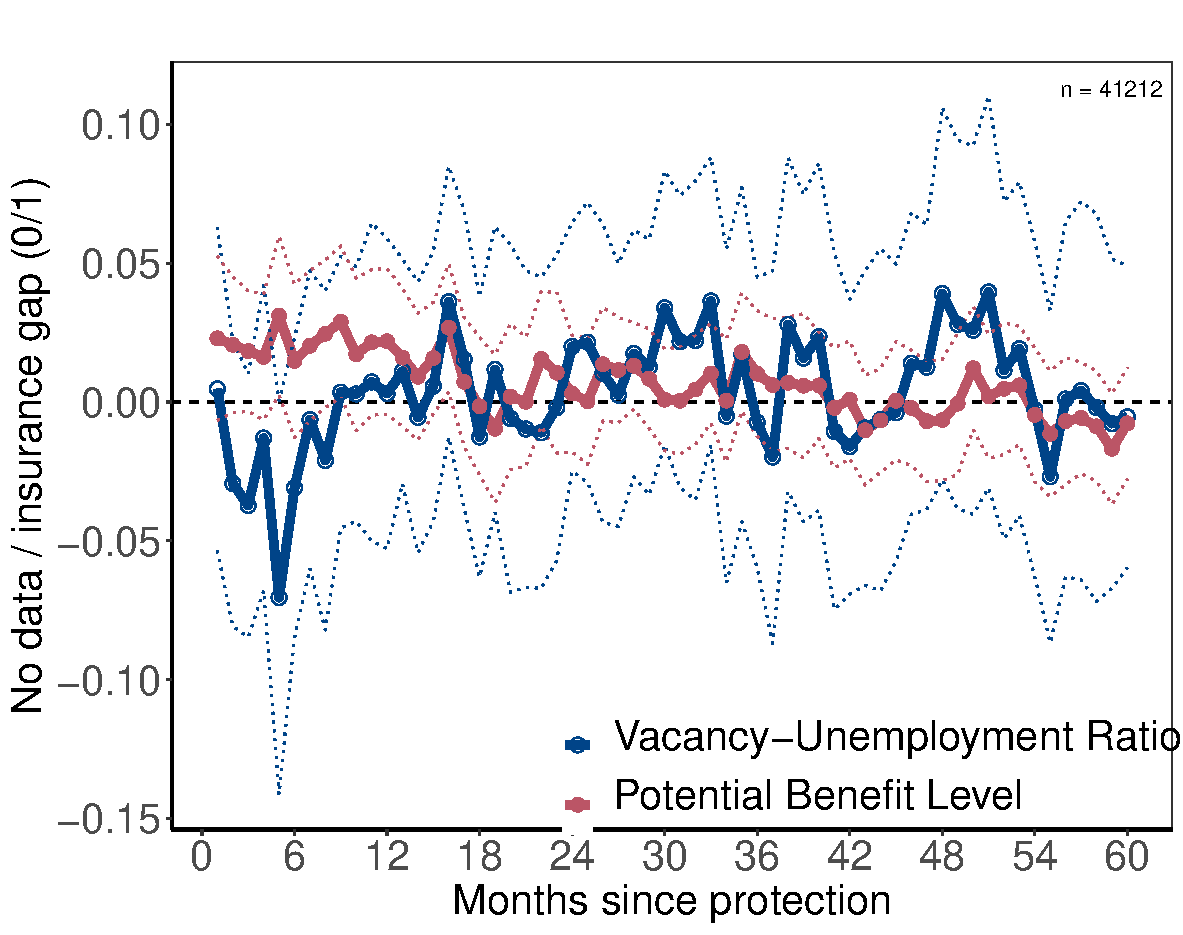
\includegraphics[scale=0.6]{figures/fig_no_data_gap.pdf}
    \end{center}
    \vspace{-0.5em}
    \fignote{\footnotesize \textit{Notes:} The x-axis shows the months since protection was received. The y-axis displays the effect of a one-unit increase in either i) the vacancy-to-unemployment ratio or ii) the potential benefit level, measured in €1,000 (real 2015 values) on having an active social insurance spell. All regressions include a full set of arrival-group, year-month, and district-of-protection fixed effects. Additional control variables include age and age squared at immigration, gender, type of protection, family status at protection date, and country of origin (see Equation \ref{eq:main}). Standard errors are clustered at the state-year-of-protection level. Dashed lines indicate 95\% confidence intervals.}
\end{figure}


%Still, this implies that our coverage of individuals with protection status is not universal. In Appendix table \ref{table:amsbmistatus}, we demonstrate that how our data aligns with the official asylum statistics.%\footnote{This table is based on an older data version from 2022. In our main sample the share of captured refugees might be slightly higher.}
%Column (1) and (2) compare the number of new asylum-seekers in the ASSD and the asylum statistics. The average coverage throughout all the sample years is 78\%. The coverage is higher for the major asylum years (2015--2016), where it reaches 92\%. Column (4) and (5) compare the number of Geneva Convention (GC) refugees registered with the AMS and the asylum statistics. Columns (7) and (8) show the respective comparison for subsidiary-protected . Note that the asylum statistics contain individuals of all ages while those registered with the AMS are of working age. Thus, we do not expect a near universal coverage. Differences in the coverage rates over time and between groups are most likely due to differences in demographics. Still, we provide evidence that the share registered with the AMS is not a function of our treatments of interest, which would raise concerns of selection bias (TBD).


% TABLE A1

\begin{figure}
\centering
    \caption{Shares and means of selected outcome variables for refugees by months since protection was received}
    \label{fig:descriptive_outcomes_appendix}
    \begin{center}        
        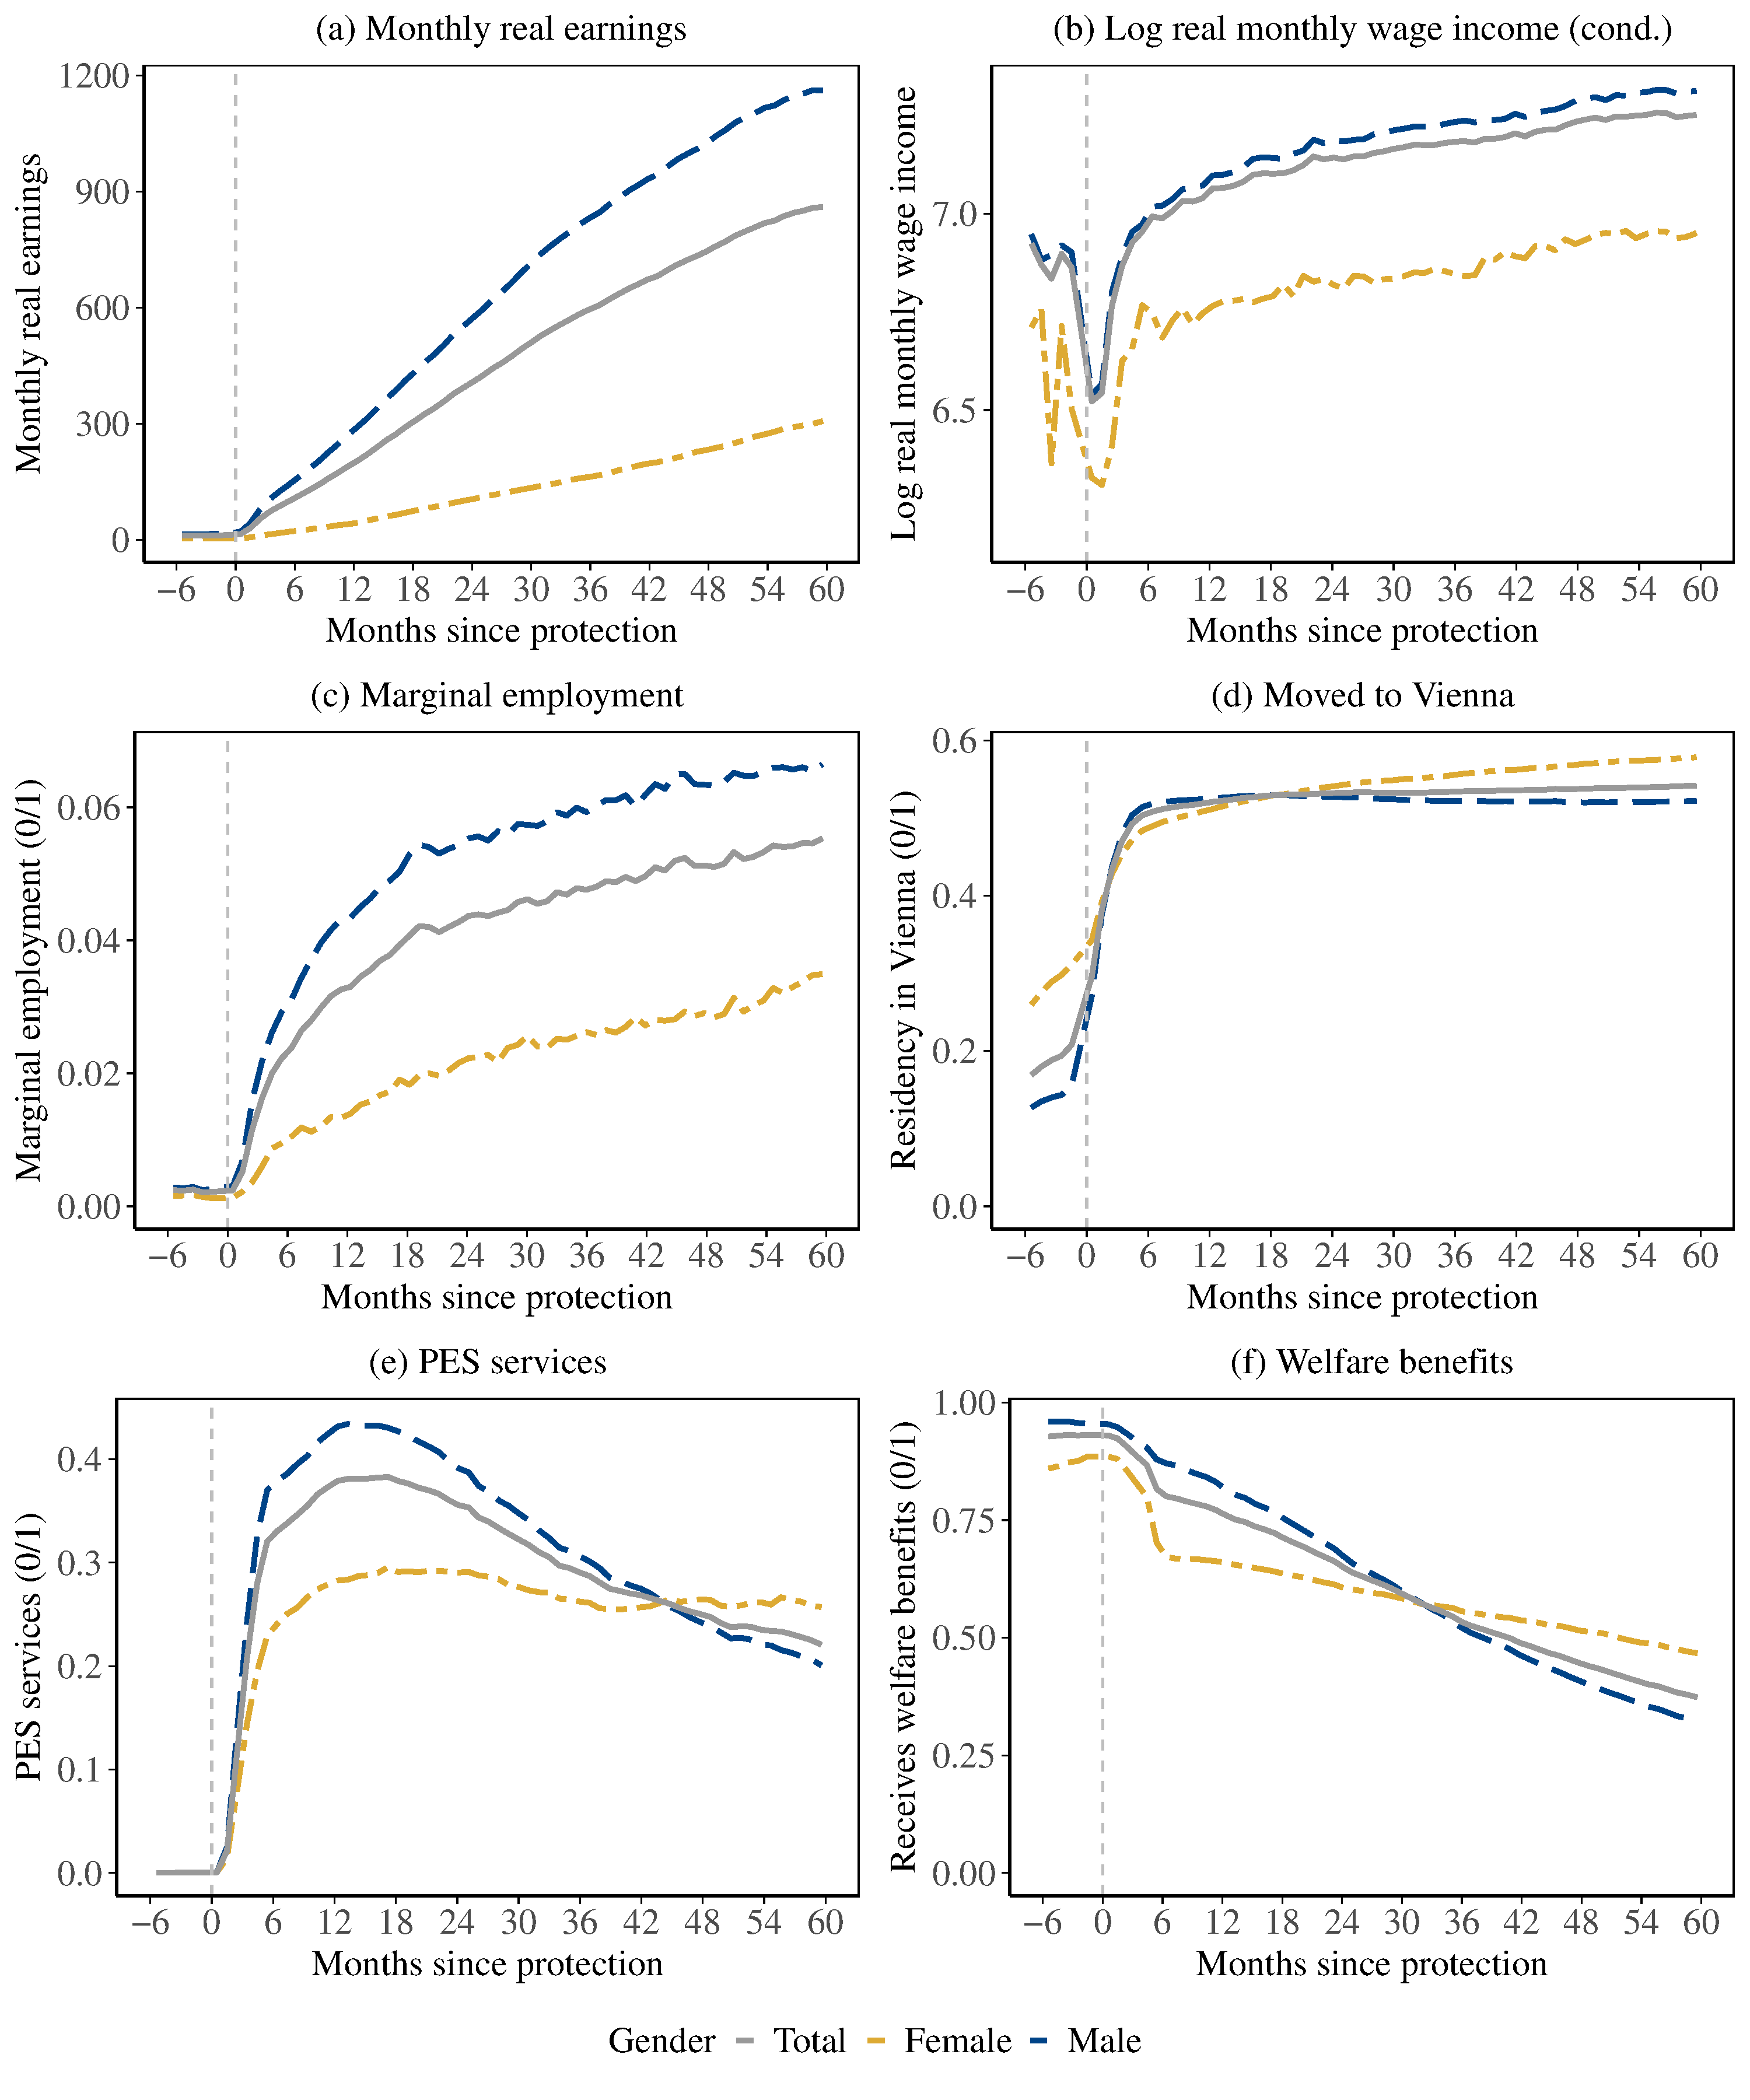
\includegraphics[scale=0.3]{figures/fig_descriptive_outcomes_appendix.pdf}
    \end{center}
    \justify
\fignote{\footnotesize \textit{Notes:} The x-axis shows the months since protection was received. The y-axis displays either the means of (a) monthly real earnings (in 2015€) and (b) log real monthly wage income (conditional on receiving any income) or the shares of refugees in (c) marginal employment, (d) residing in Vienna, (e) receiving support by the PES and (f) receiving basic needs support, by gender.}
\end{figure}


\begin{figure}
    \caption{Effect of the IVUR and IPBL on selected outcomes: Asylum until 2021}
    \label{fig:robustness_asylum2021}
    \begin{center}
    %\vspace{-0.5 cm}
    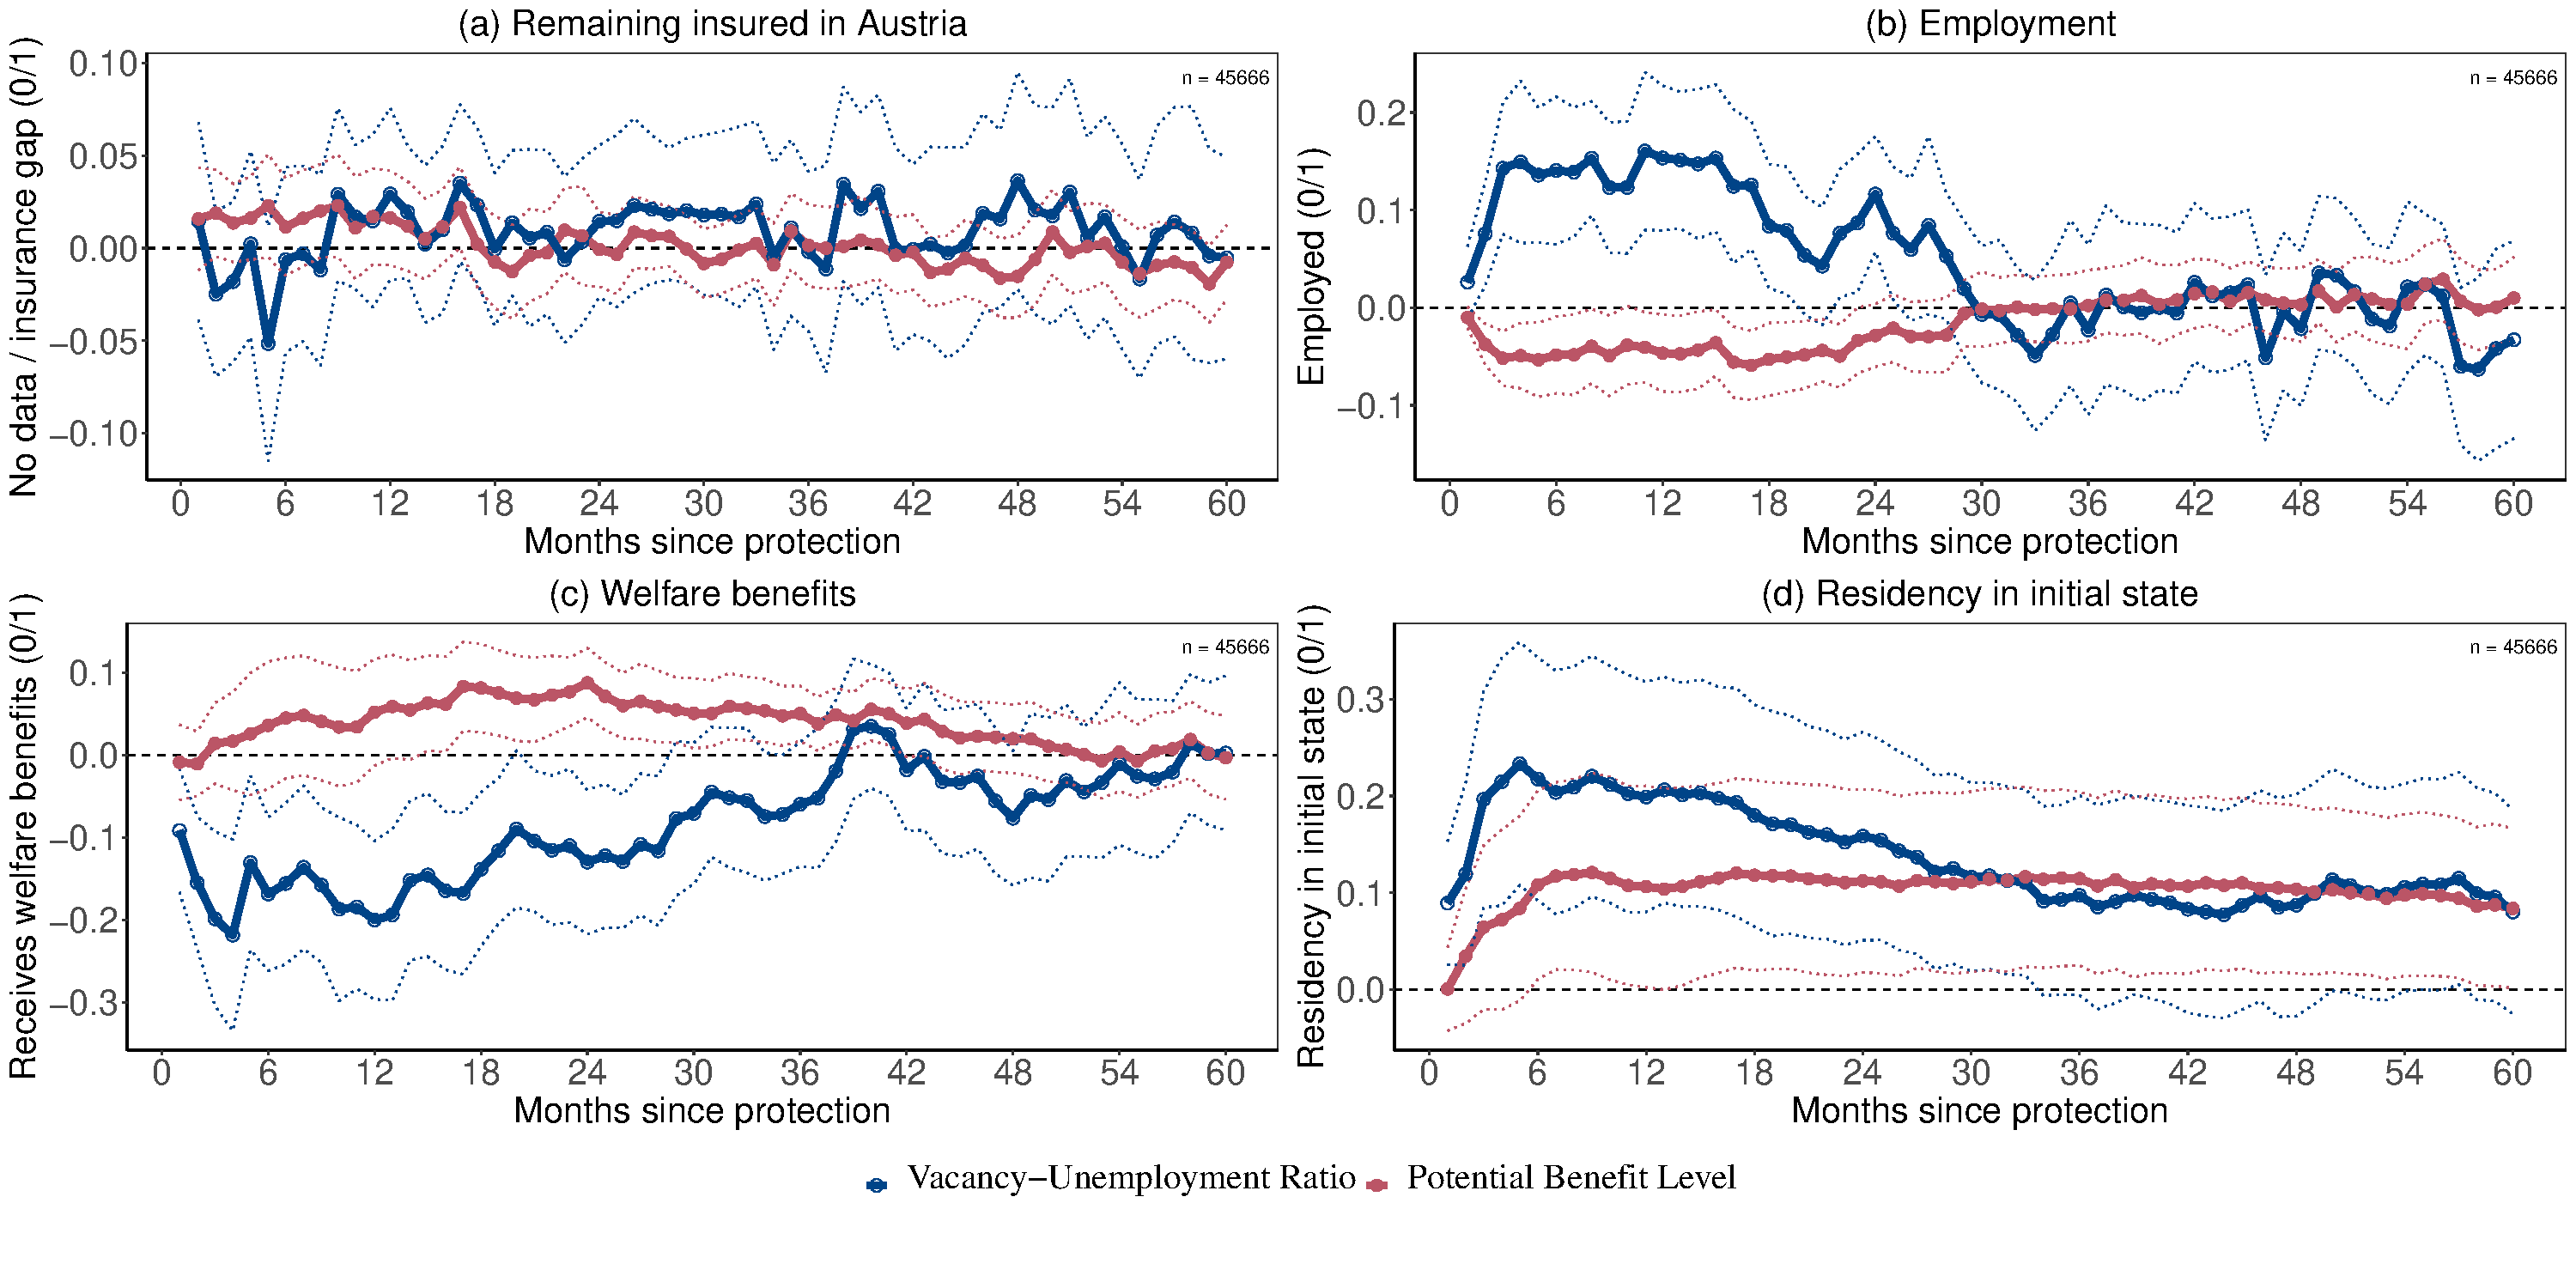
\includegraphics[scale=0.31]{figures/fig_incl_short_horizon.pdf}
    \end{center}
    \fignote{\footnotesize \textit{Notes:} This figure shows selected main outcomes without placing restrictions on being observed for 60 months yet. The x-axis shows the months since protection was received. The y-axis displays the effect of a one-unit increase in either i) the vacancy-unemployment ratio or ii) the potential benefit level, measured in €1,000 (real 2015 values), on selected outcomes. The panels show the effects on (a) remaining insured in Austria; panel (b) having any type of part- or full-time employment; panel (c) the probability of receiving welfare benefits; and panel (d) the probability of living in the initial political district. All regressions include a full set of arrival-group, year-month, and district-of-protection fixed effects. Additional control variables include age and age squared at immigration, gender, type of protection, family status at protection date, and country of origin. Standard errors are clustered at the state-year-of-protection level. Dashed lines indicate 95\% confidence intervals.}
\end{figure}



\begin{figure}
    \caption{Effect of the $IVUR$ and $IPBL$ on employment and location choice for those who initially lived in a reception facility}
    \label{fig:rob_labor_mobility_initial_facility}
    \begin{center}
    %\vspace{-0.5 cm}
    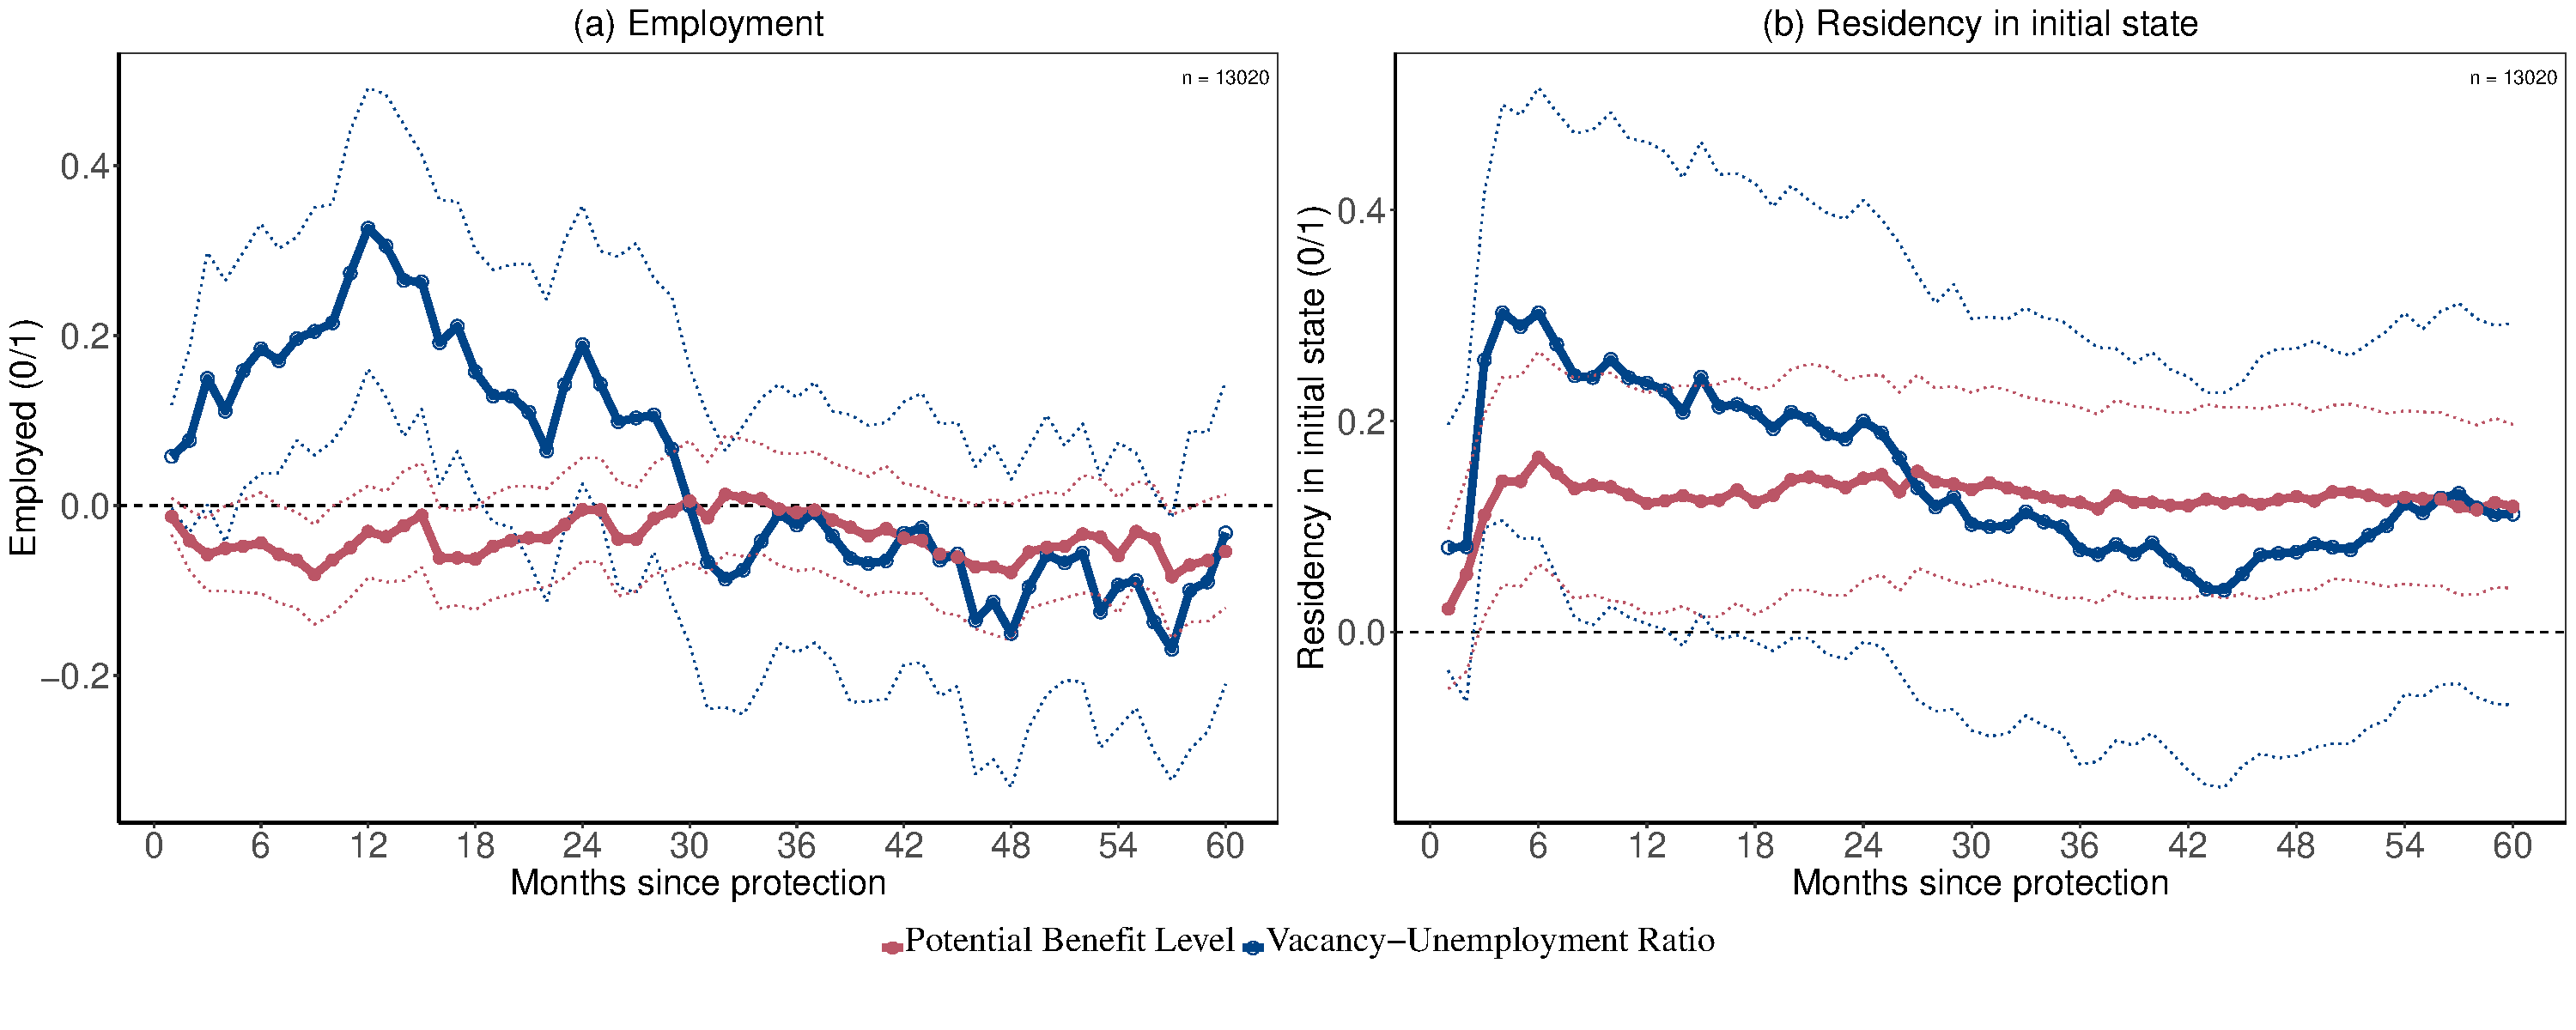
\includegraphics[scale=0.31]{figures/rob/fig_rob_labor_mobility_initial_facility.pdf}
    \end{center}
    \fignote{\footnotesize \textit{Notes:} The x-axis shows the months since protection was received. The y-axis displays the effect of a one-unit increase in either i) the vacancy-to-unemployment ratio or ii) the potential benefit level, measured in €1,000 (real 2015 values), on employment (left) and mobility (right). All regressions include a full set of arrival-group, year-month, and district-of-protection fixed effects. Additional control variables include age and age squared at immigration, gender, type of protection, family status at protection date, and country of origin. Standard errors are clustered at the state-year-of-protection level. Dashed lines indicate 95\% confidence intervals.}
\end{figure}

\begin{figure}
    \caption{Effect of the $IVUR$ and $IPBL$ on employment and location choice for those with asylum processes longer than one month}
    \label{fig:rob_labor_mobility_process_more1month}
    \begin{center}
    %\vspace{-0.5 cm}
    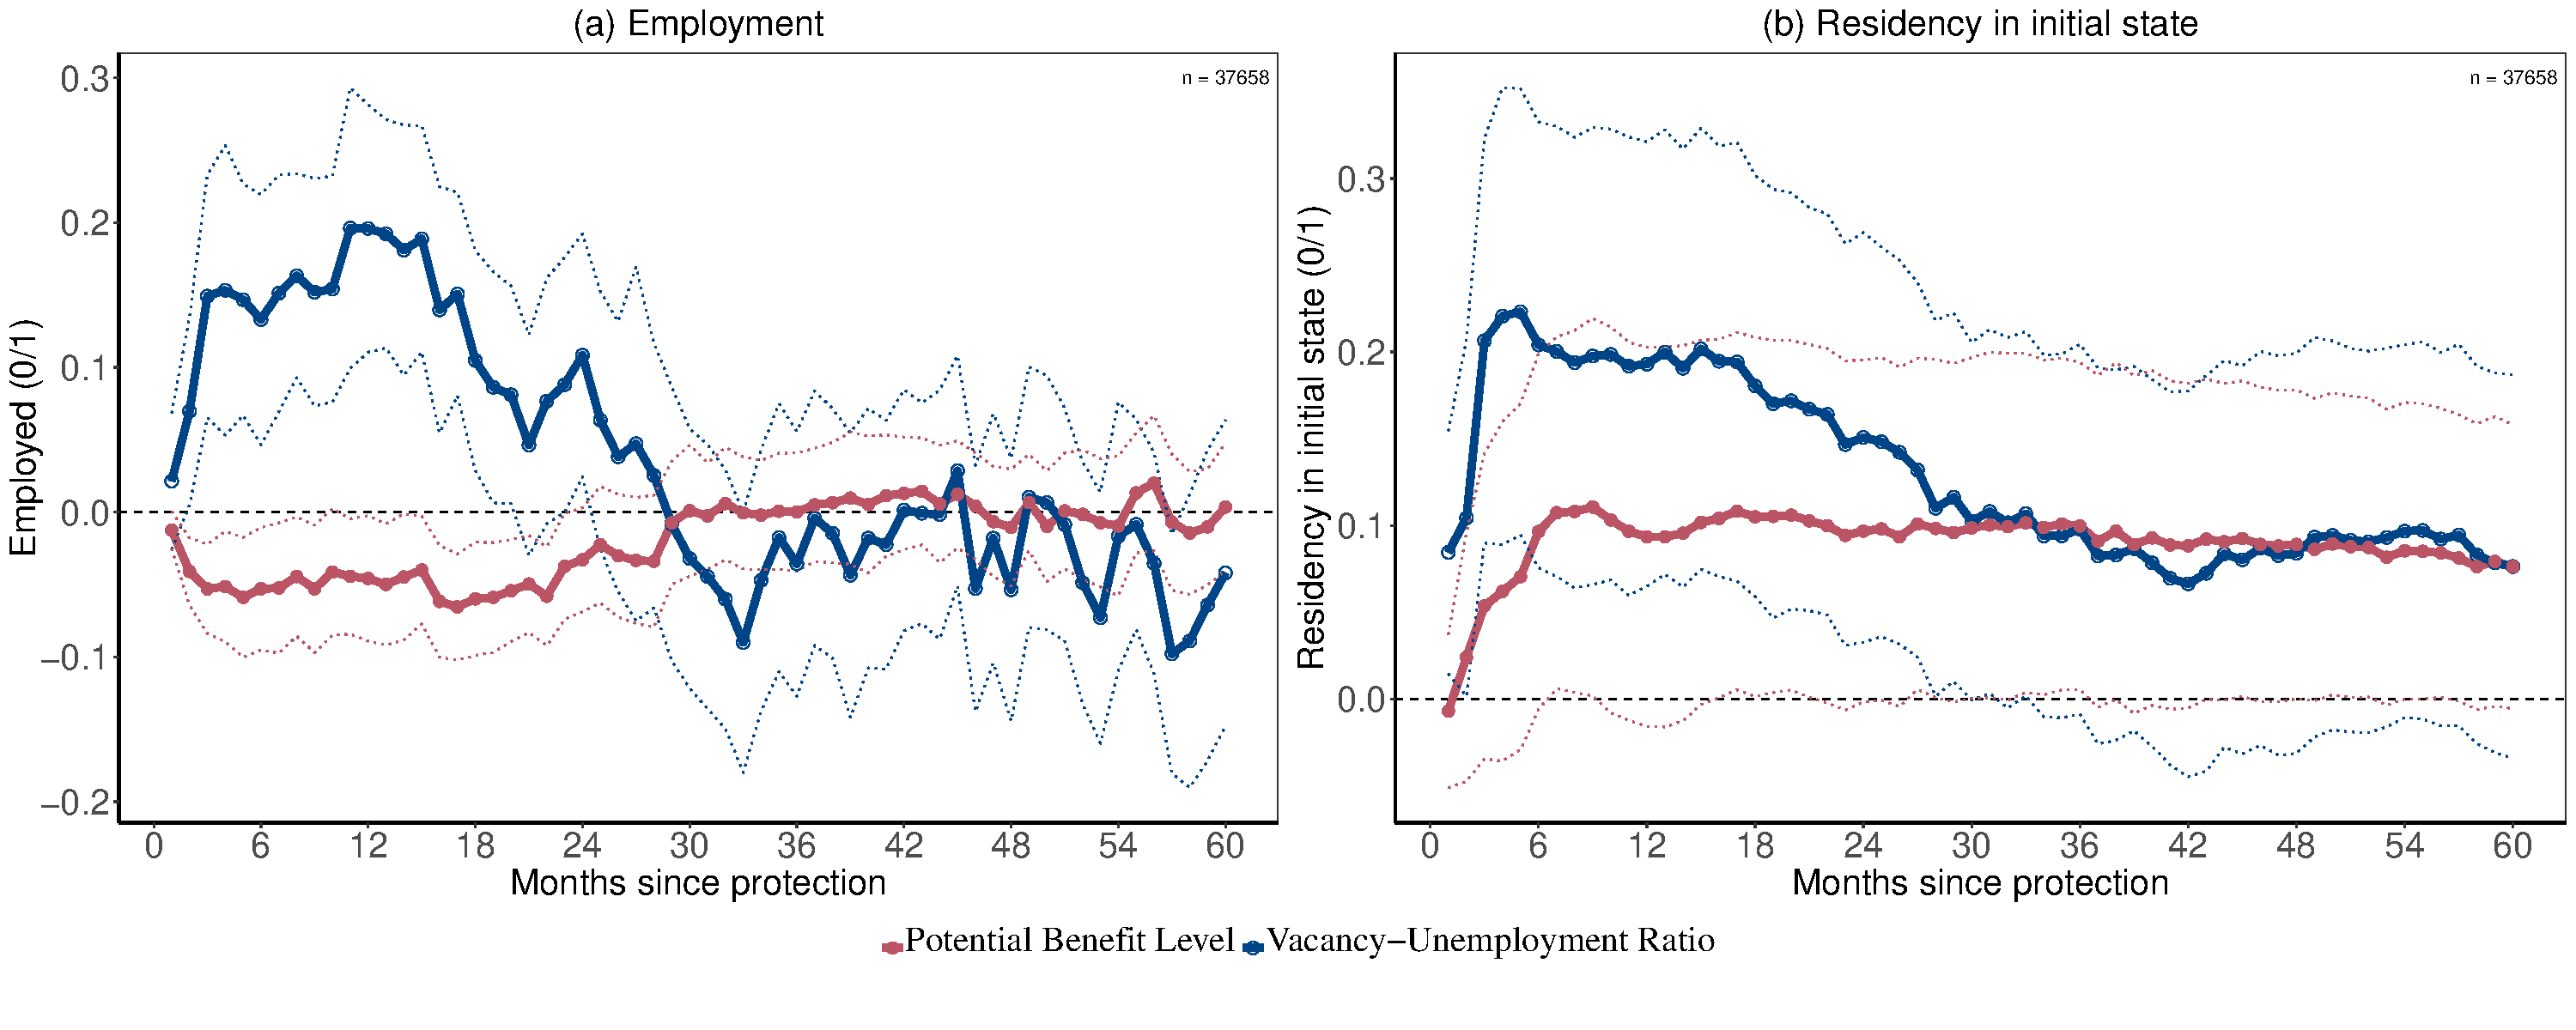
\includegraphics[scale=0.31]{figures/rob/fig_rob_labor_mobility_process_more1month.pdf}
    \end{center}
    \fignote{\footnotesize \textit{Notes:} The x-axis shows the months since protection was received. The y-axis displays the effect of a one-unit increase in either i) the vacancy-to-unemployment ratio or ii) the potential benefit level, measured in €1,000 (real 2015 values), on employment (left) and mobility (right). All regressions include a full set of arrival-group, year-month, and district-of-protection fixed effects. Additional control variables include age and age squared at immigration, gender, type of protection, family status at protection date, and country of origin. Standard errors are clustered at the state-year-of-protection level. Dashed lines indicate 95\% confidence intervals.}
\end{figure}


\begin{figure}
    \caption{Effect of the $IVUR$ and $IPBL$ on employment and location choice excluding protection within four months of reform}
    \label{fig:rob_labor_mobility_noreform_4month}
    \begin{center}
    %\vspace{-0.5 cm}
    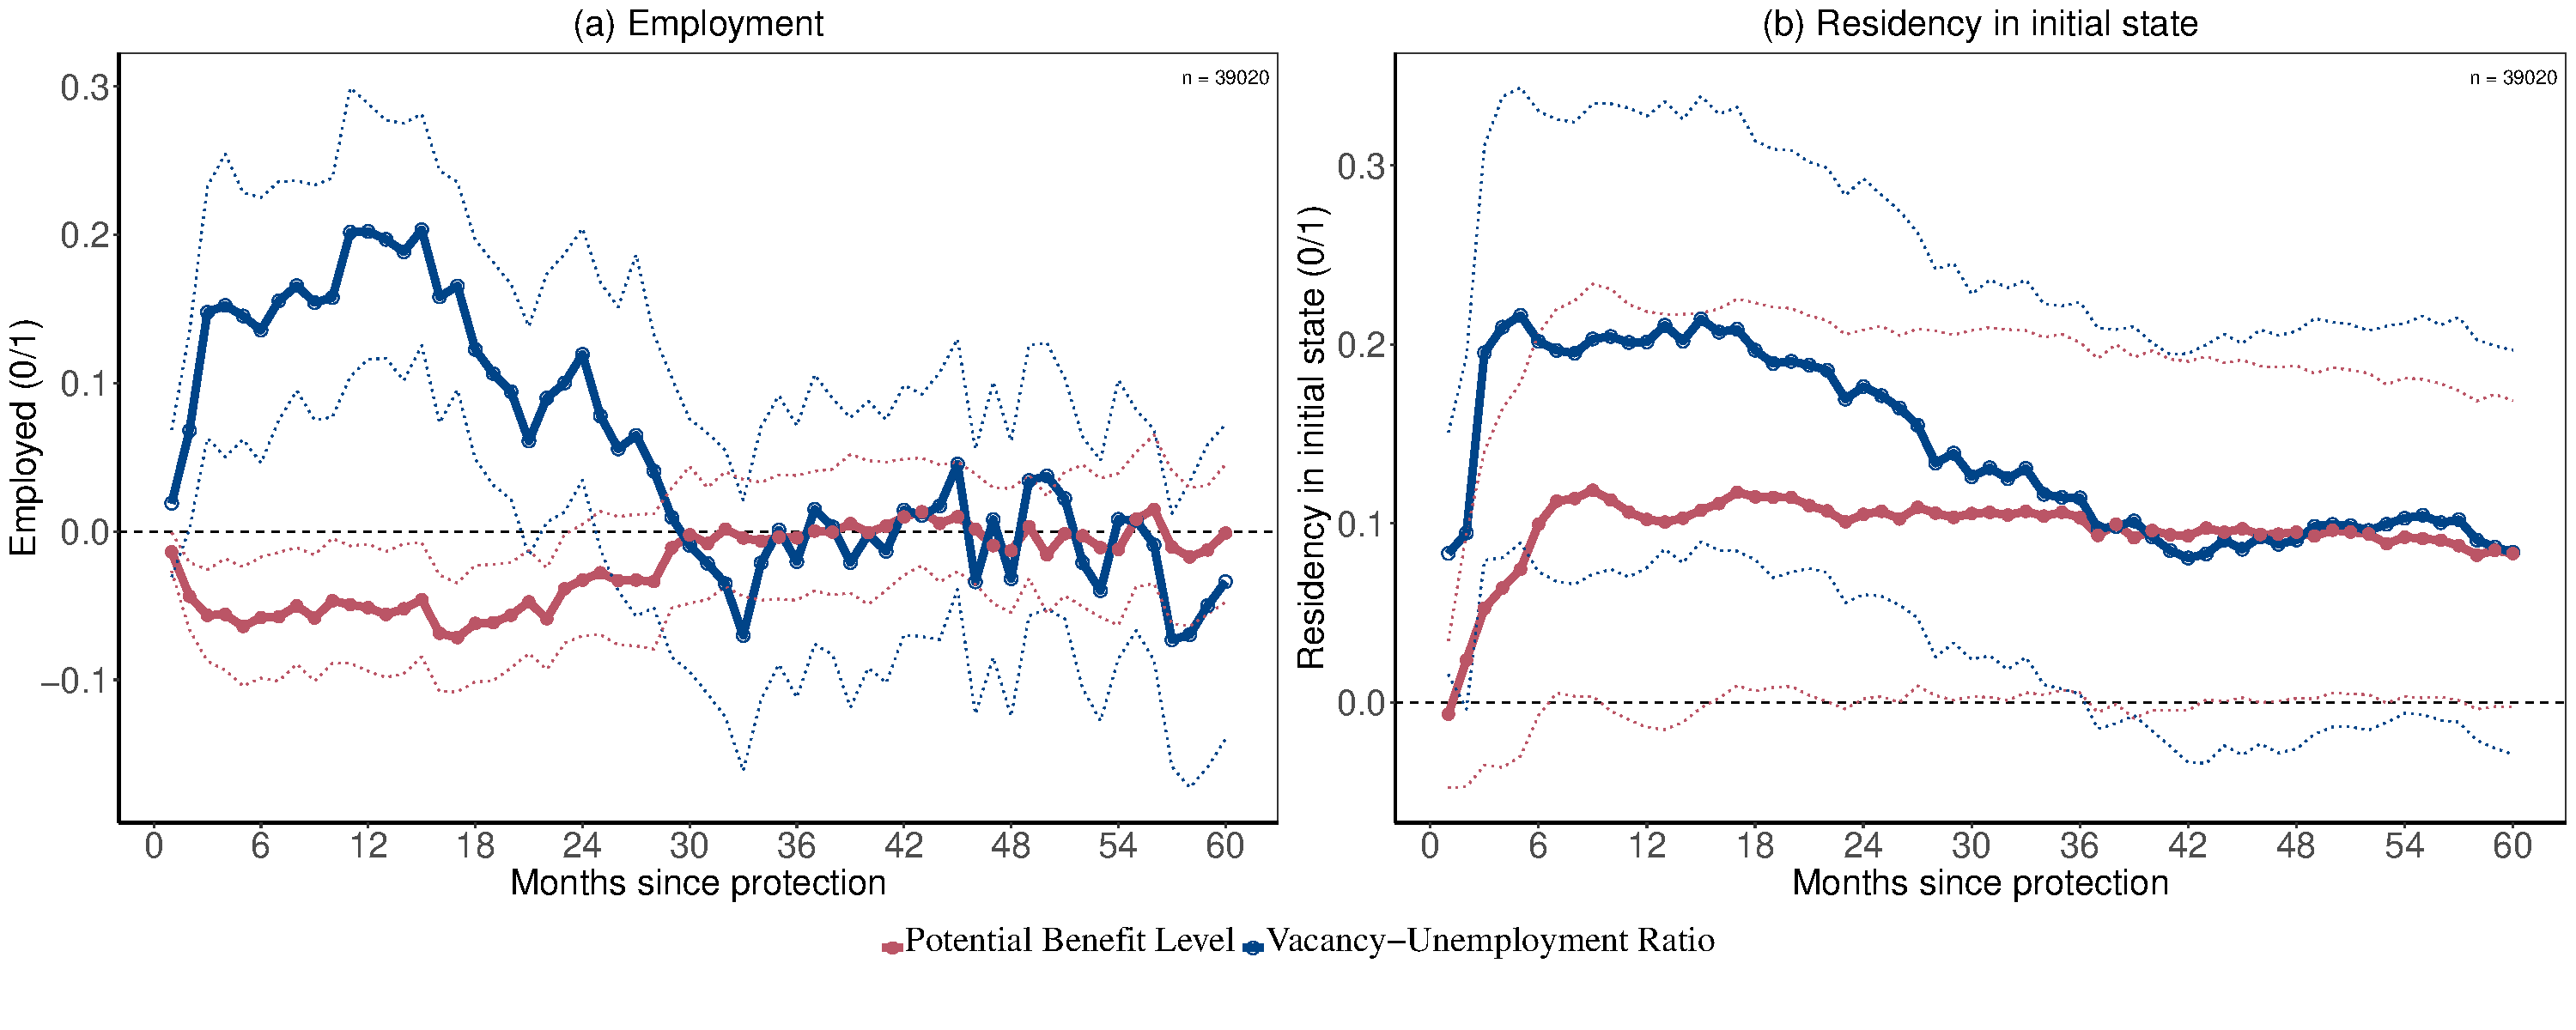
\includegraphics[scale=0.31]{figures/rob/fig_rob_labor_mobility_noreform_4month.pdf}
    \end{center}
    \fignote{\footnotesize \textit{Notes:} The x-axis shows the months since protection was received. The y-axis displays the effect of a one-unit increase in either i) the vacancy-to-unemployment ratio or ii) the potential benefit level, measured in €1,000 (real 2015 values), on employment (left) and mobility (right). All regressions include a full set of arrival-group, year-month, and district-of-protection fixed effects. Additional control variables include age and age squared at immigration, gender, type of protection, family status at protection date, and country of origin. Standard errors are clustered at the state-year-of-protection level. Dashed lines indicate 95\% confidence intervals.}
\end{figure}

\begin{figure}
    \caption{Effect of the $IVUR$ and $IPBL$ on employment and location choice for those who lived in their state at least one month prior to receiving protection}
    \label{fig:rob_labor_mobility_state_approval_min1month}
    \begin{center}
    %\vspace{-0.5 cm}
    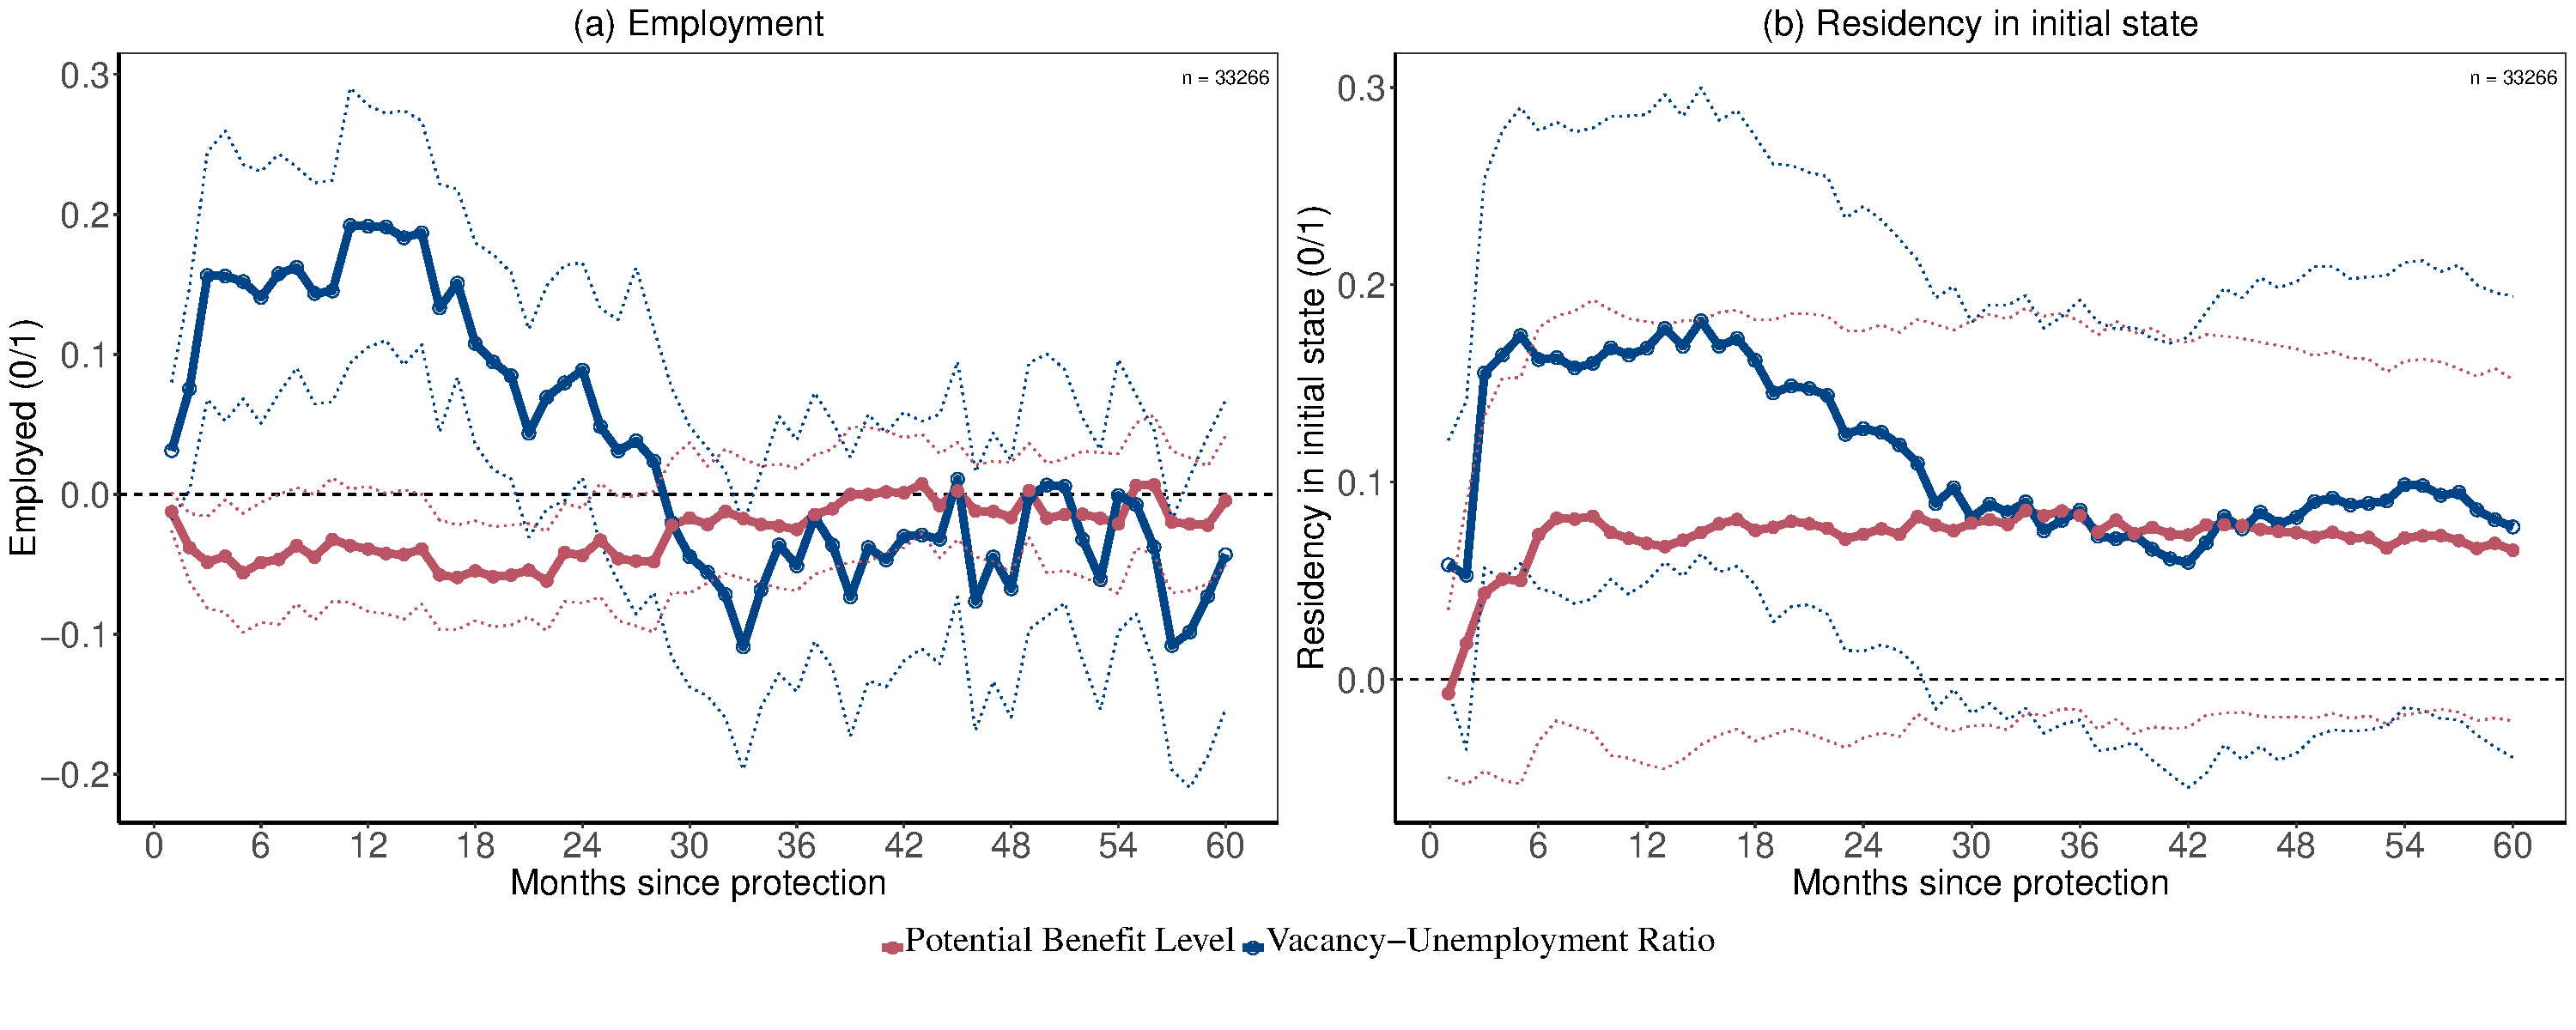
\includegraphics[scale=0.31]{figures/rob/fig_rob_labor_mobility_state_approval_min1month.pdf}
    \end{center}
    \fignote{\footnotesize \textit{Notes:} The x-axis shows the months since protection was received. The y-axis displays the effect of a one-unit increase in either i) the vacancy-to-unemployment ratio or ii) the potential benefit level, measured in €1,000 (real 2015 values), on employment (left) and mobility (right). All regressions include a full set of arrival-group, year-month, and district-of-protection fixed effects. Additional control variables include age and age squared at immigration, gender, type of protection, family status at protection date, and country of origin. Standard errors are clustered at the state-year-of-protection level. Dashed lines indicate 95\% confidence intervals.}
\end{figure}


\begin{figure}
    \caption{Effect of the $IVUR$ and $IPBL$ on employment and location choice with year and month fixed effects}
    \label{fig:rob_labor_mobility_year_month_fe}
    \begin{center}
    %\vspace{-0.5 cm}
    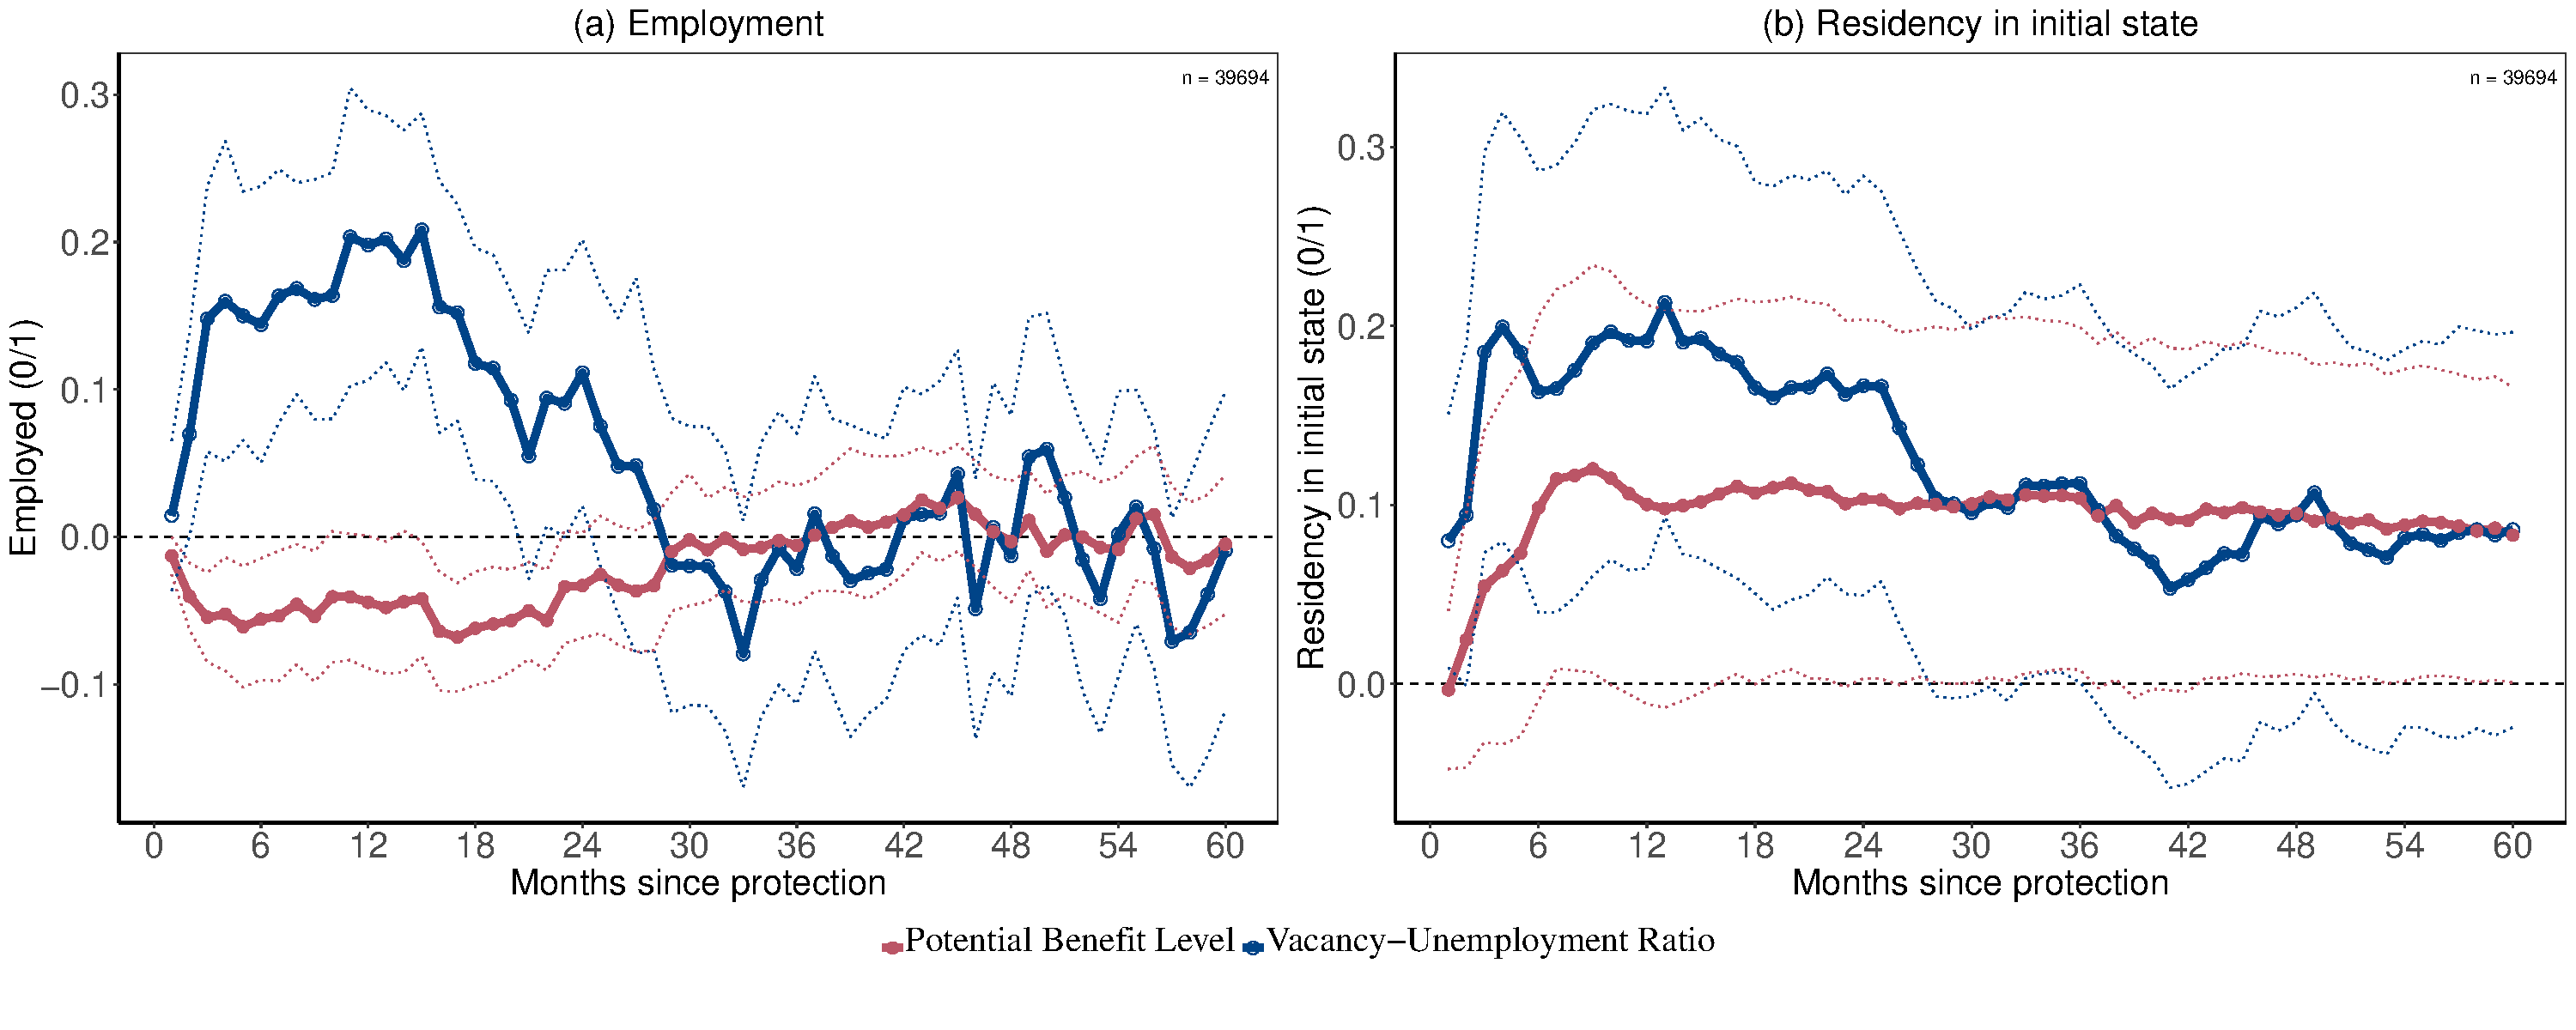
\includegraphics[scale=0.31]{figures/rob/fig_rob_labor_mobility_year_month_fe.pdf}
    \end{center}
    \fignote{\footnotesize \textit{Notes:} The x-axis shows the months since protection was received. The y-axis displays the effect of a one-unit increase in either i) the vacancy-to-unemployment ratio or ii) the potential benefit level, measured in €1,000 (real 2015 values), on employment (left) and mobility (right). All regressions include a full set of arrival-group, year-month, and district-of-protection fixed effects. Additional control variables include age and age squared at immigration, gender, type of protection, family status at protection date, and country of origin. Standard errors are clustered at the state-year-of-protection level. Dashed lines indicate 95\% confidence intervals.}
\end{figure}


\begin{figure}
    \caption{Robustness: Different Standard Errors and Wild Cluster Bootstrap}
    \label{fig:errors_all}
    \begin{center}
    \vspace{-0.5 cm}
    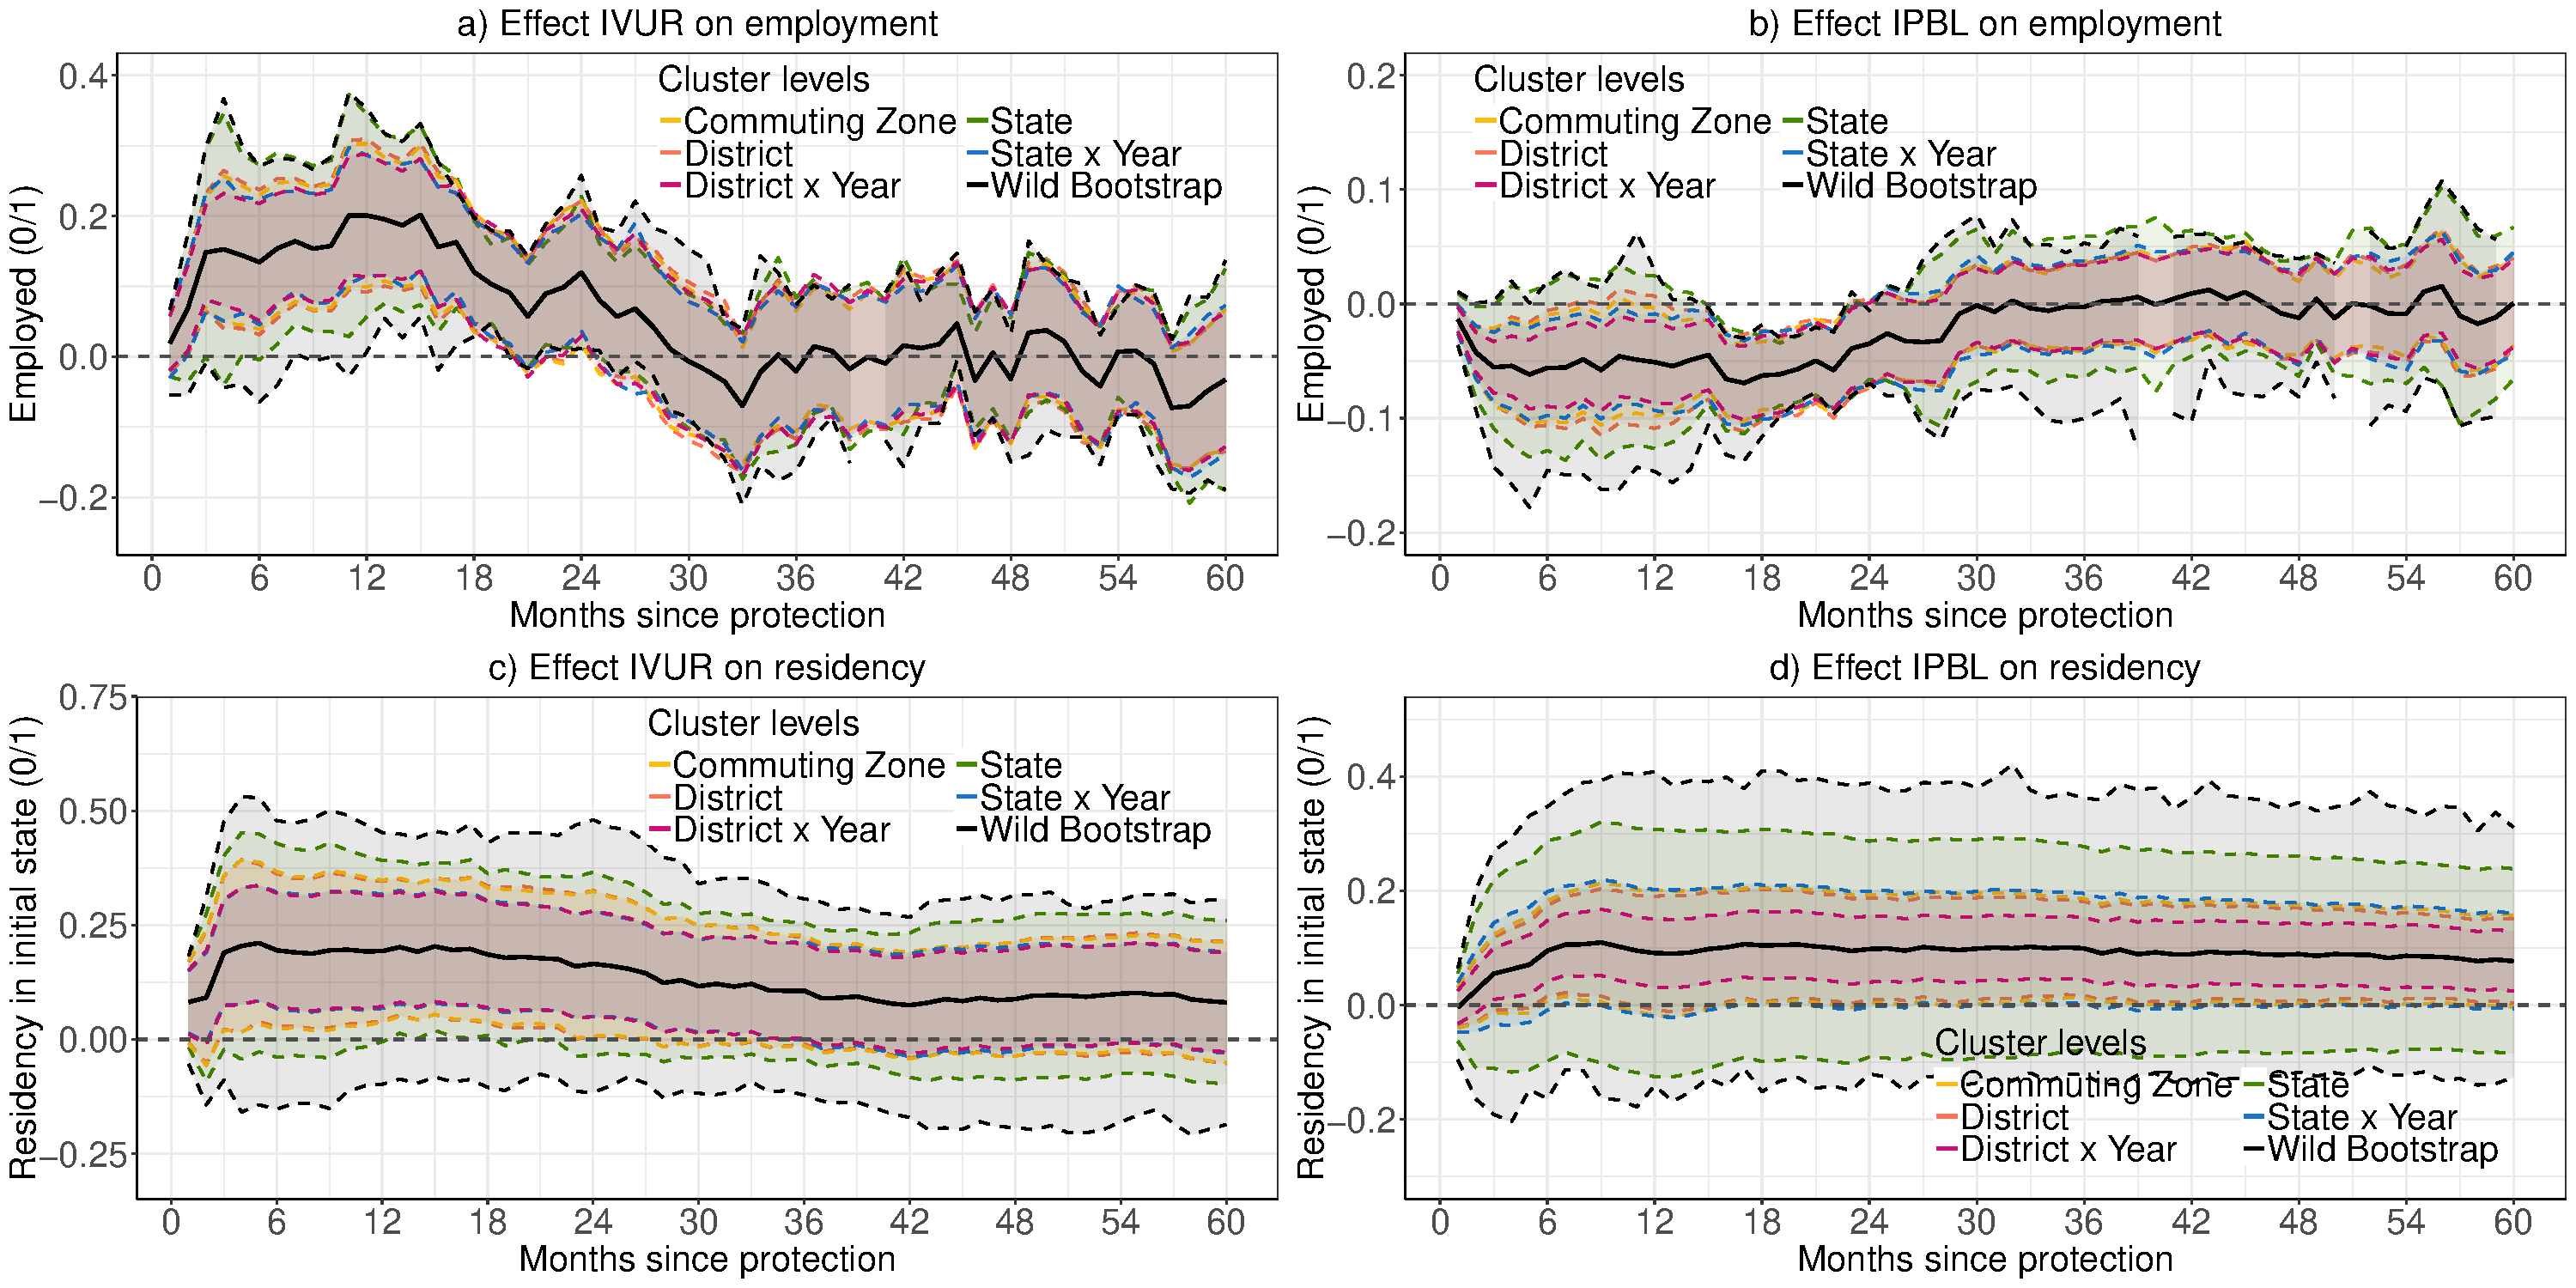
\includegraphics[scale=0.31]{figures/rob/different_standard_errors_all.pdf}
    \end{center}
    \vspace{-0.5 cm}
    \fignote{\footnotesize \textit{Notes:} Comparison of the estimated effects of the vacancy-to-unemployment ratio (left) and the potential benefit level (right) on employment (top row) and residency in the state of protection (bottom row). Each plot shows the point estimates and confidence intervals using standard errors clustered at alternative aggregation levels (district, state, commuting zone, state~$\times$~year, district~$\times$~year), as well as wild cluster bootstrap intervals. Each dotted pair of confidence intervals corresponds to a different clustering level for the calculation of standard errors. Black lines indicate confidence intervals from wild cluster bootstrap procedures using Rademacher weights for the IVUR and Webb weights for the IPBL.}
\end{figure}



\begin{figure}
    \caption{Robustness: Leave-One-Nationality-Out Analysis}
    \label{fig:leavenats}
    \begin{center}
    \vspace{-0.5 cm}
    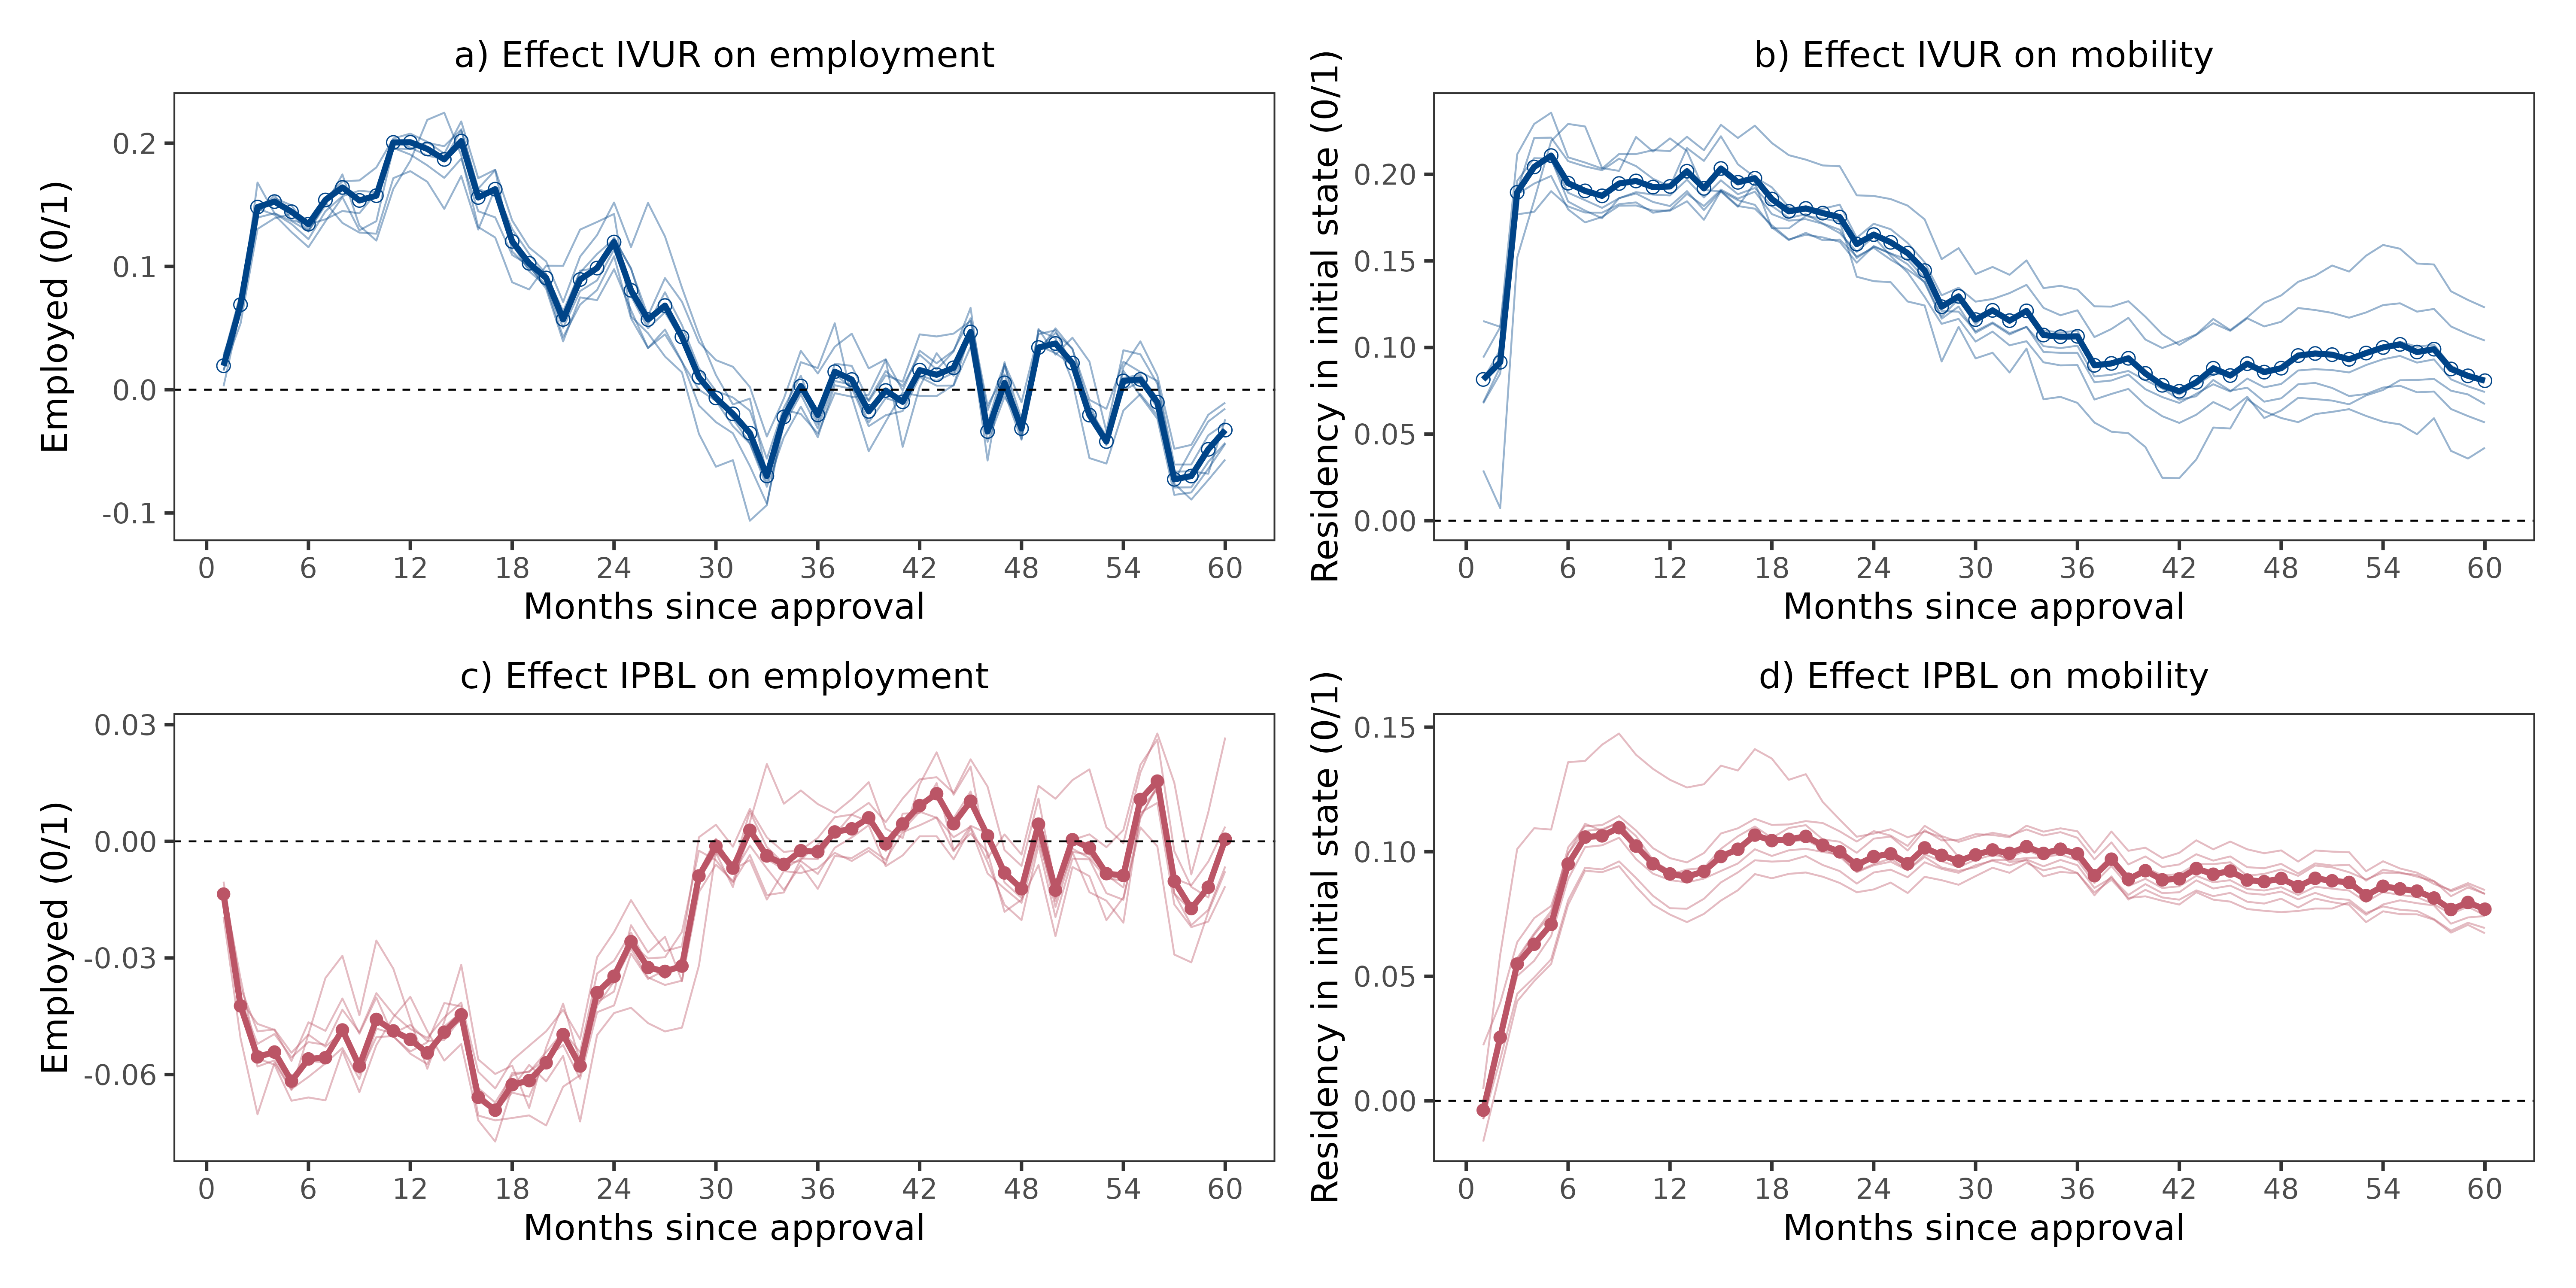
\includegraphics[scale=0.31]{figures/rob/leavenationality_fourplots.png}
    \end{center}
    \vspace{-0.5 cm}
    \fignote{\footnotesize \textit{Notes:} The thick lines correspond to the main results from figures \ref{fig:mobility_results} (a) and \ref{fig:empl_reloc} (a). Each thin line corresponds to re-estimating the main model after excluding one nationality group from the sample.}
\end{figure}




\begin{figure}
    \caption{Robustness: Leave-One-State-Out Analysis}
    \label{fig:leavestates}
    \begin{center}
    \vspace{-0.5 cm}
    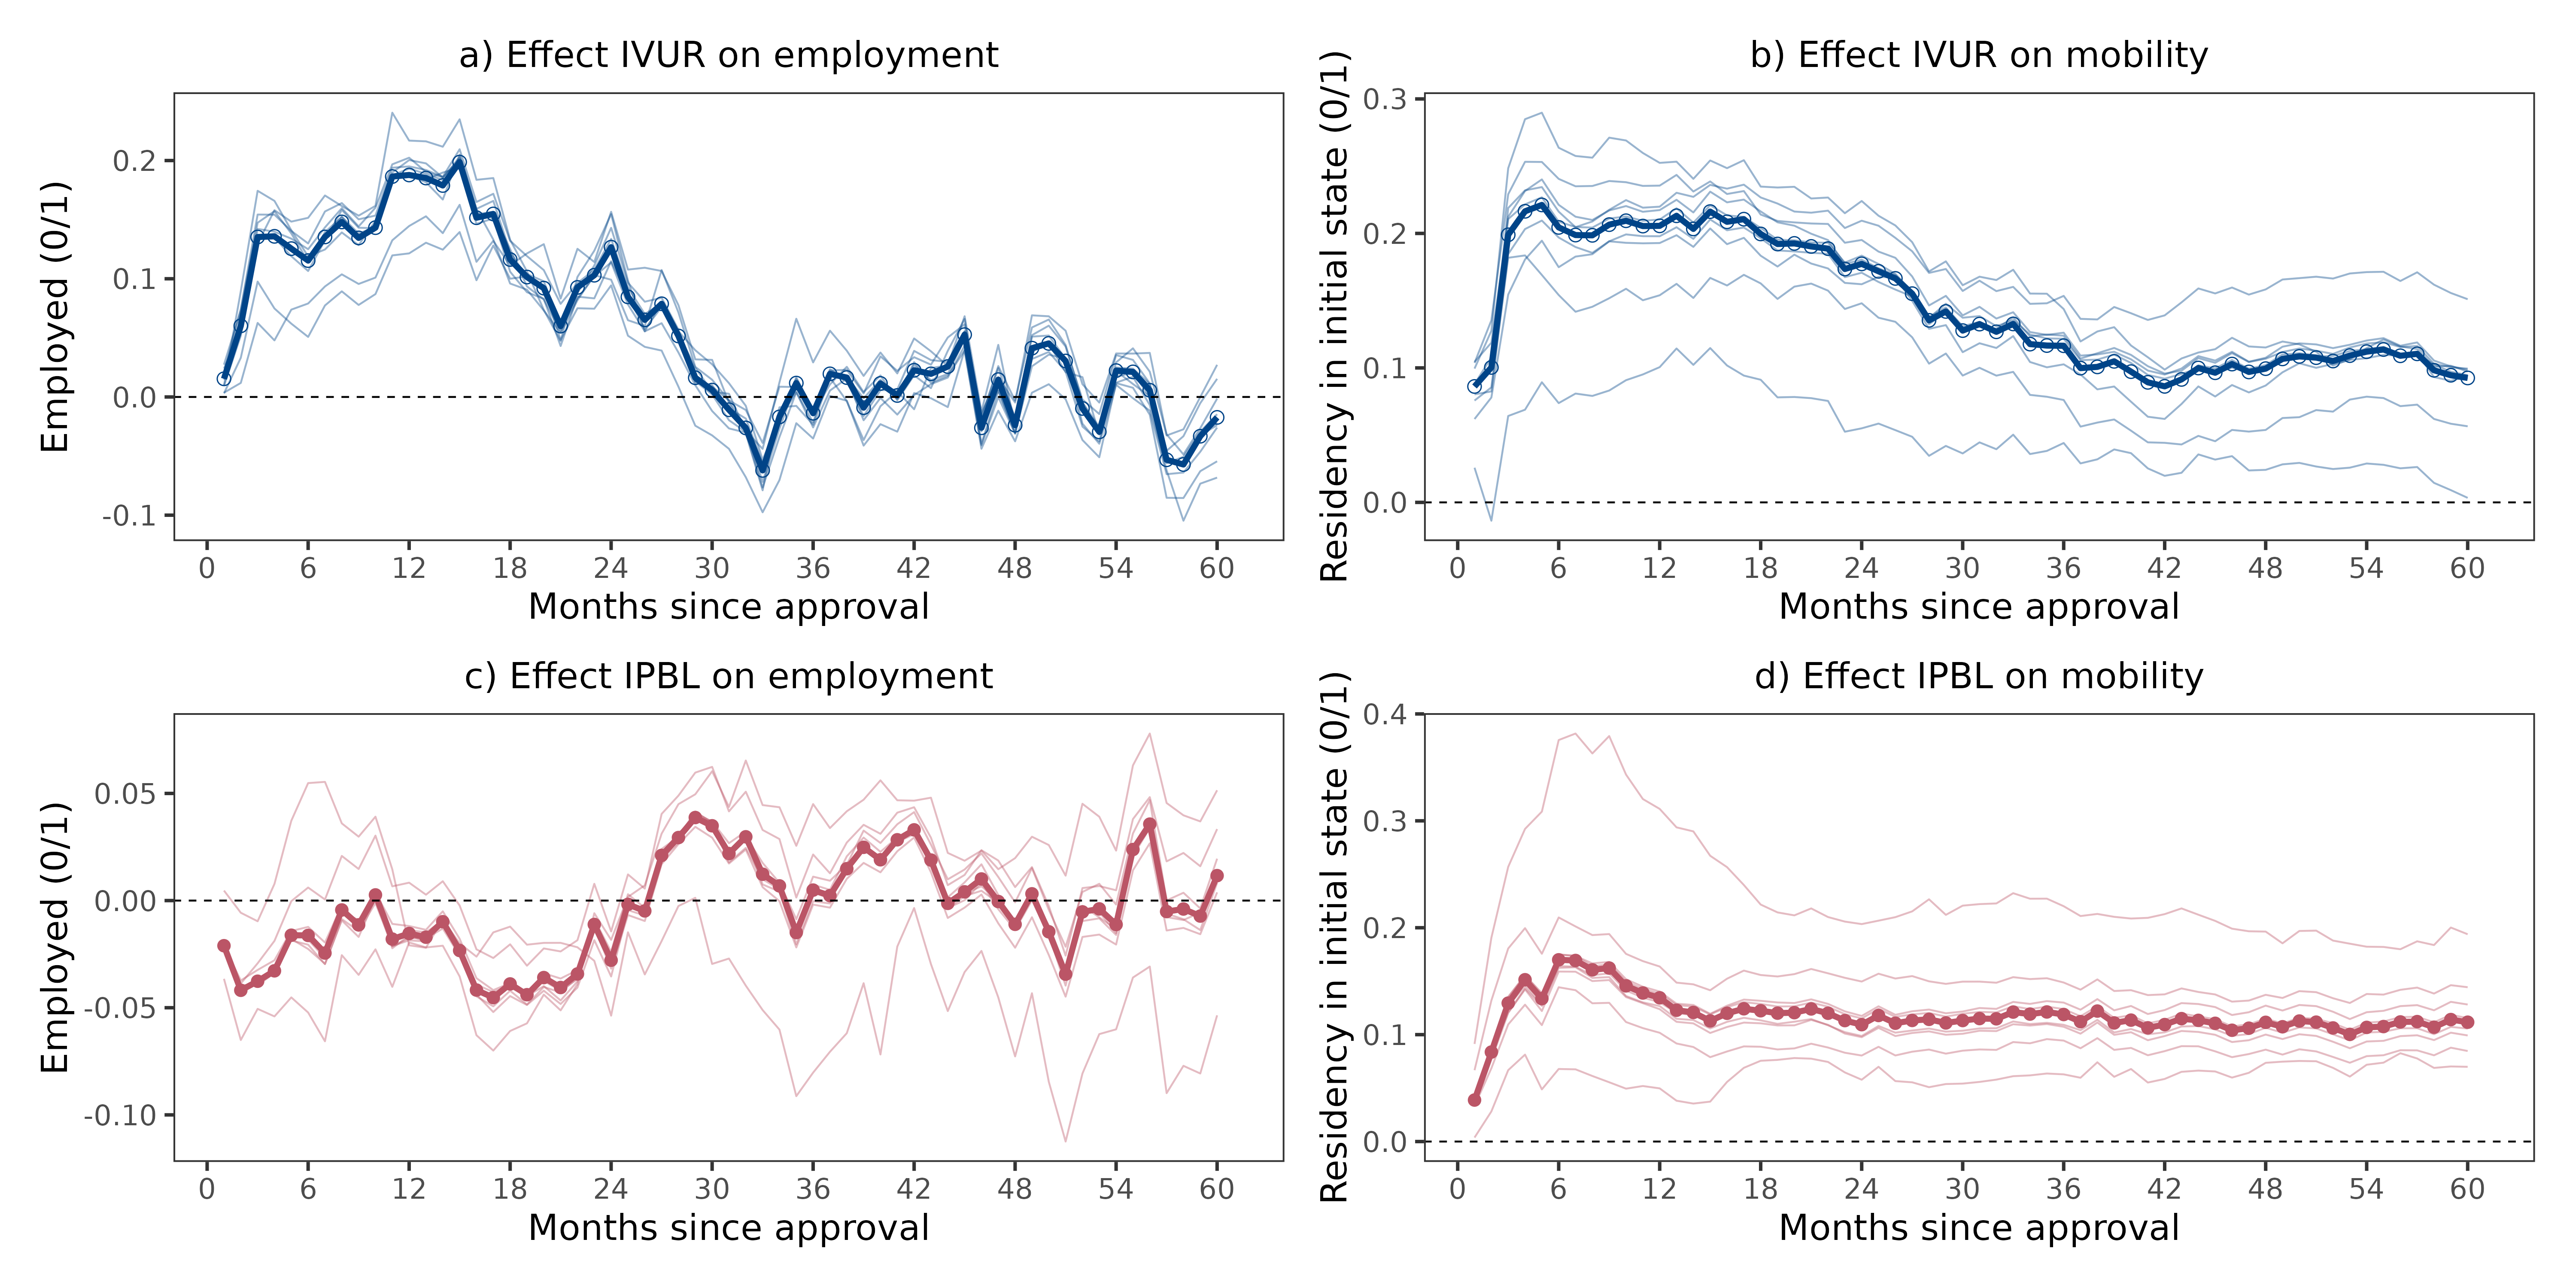
\includegraphics[scale=0.31]{figures/rob/leavestate_fourplots_nolabel.png}
    \end{center}
    \vspace{-0.5 cm}
    \fignote{\footnotesize \textit{Notes:} The thick lines correspond to the main results from figures \ref{fig:mobility_results} (a) and \ref{fig:empl_reloc} (a). Each thin line corresponds to re-estimating the main model after excluding one state at time of protection group from the sample.}
\end{figure}




\clearpage
\section{Data Appendix} \label{sec:appendixb}
\subsection{Sample selection: registrations at the PES}\label{subsec:pes_selection}
In our dataset, we only have information on the status granted and the date of asylum for those individuals who registered at the Public Employment Services (PES). Hence, there could be a concern that our shocks (\textit{IVUR} and \textit{IPBL}) correlate with the probability of registering at the PES and might bias our results.

Using our registry data (ASSD), we collapse the number of individuals by sex and citizenship living in district \textit{d} at the moment of getting asylum by year of protection for 2011--2020. We keep only individuals from the top 8 asylum-applicant countries: Afghanistan, Iraq, Iran, Kosovo, Nigeria, Russia, Somalia, and Syria. 

We merge these collapsed headcounts of refugees with the total population of foreigners from the top 8 asylum-applicant countries at the district level as of January 1 of the following year. These are data provided by STATcube by country of birth and gender and are stocks as of January 1 of each year. For example, we merge the headcounts by protection status of those individuals who received protection in 2015 with the total population of foreigners from these countries in a district as of January 1, 2016. We then divide our ASSD headcounts on refugees by status by the total population of individuals from these eight asylum-applicant countries at the district level to obtain a share of refugees with a status among the foreign population.

Additionally, we merge the yearly averages of \textit{IVUR} at the district level and the ones from \textit{IPBL} at the state level by year of protection.
Finally, we run a regression of the share of refugees with status among the foreign population on our treatment variables, year, district, nationality, and type of protection fixed effects. 

Table \ref{tab:assd_statcube} presents these results. The first three columns show the results for shares by nationalities as outcomes, while the latter three columns use the aggregated shares for all top 8 asylum-applicant countries as outcomes. The coefficients for the \textit{IVUR} are positive but statistically not significant in columns (1)-(3). Since our dependent variable ranges from zero to one, a one unit increase in the $IVUR$ would increase the share of (registered) refugees in a district by 2.4 pp. To put this in standard increase terms, as in our main analysis, a 0.2 units increase in the $IVUR$ would increase the share of registered refugees by 0.4 pp., which is relatively small compared to the effect sizes we find in our main specification. In columns (4)-(5), where we use the overall shares as an outcome, the effect of the $IVUR$ becomes statistically significant at the 5\% level. This positive relation hints at a positive effect of $IVUR$ on registration with the PES. If the individuals who register when the labor market is tight but not otherwise are individuals who are relatively more inclined to take up employment, our estimates for the effect of $IVUR$ on employment might be upward biased. However, the magnitude of such a bias is minor.

For the $IPBL$, the only significant coefficient is the one for the family benefits on the share of registered females in column (2) but not when aggregating the shares across nationalities. Given the low share of singles and the low employment rates for women, they do indeed mostly qualify for family benefits. Thus, higher benefit levels might indeed have increased the incentive to register at the PES in order to receive benefits. These positive benefits effects on the registration of female refugees might bias our estimates of $IPBL$ on benefit receipt upward and on employment downwards. However, since the effect is again small in magnitude, we consider the size of such potential biases again to be minor.

Overall, these effects are small and only significant for females, who represent 30\% of our sample. They could, however, indicate an upward bias of our effects. 

\begin{table}
\centering
	\caption{Correlation of initial vacancy-to-unemployment ratio and initial potential benefit level with the share of refugees in a district}
	\label{tab:assd_statcube}
	\begin{threeparttable}
 \centering
		%\begin{small}
			\centering
\begin{tabular}{lcccccc}
\hline
            & (1) & (2) & (3)  & (4) & (5) & (6)  \\
            & \multicolumn{3}{c}{Shares by nationalities} & \multicolumn{3}{c}{Aggregated shares} \\
            & All & Females & Males & All & Females & Males \\ \hline
IVUR            & 0.0237  & 0.0329  &  0.0423 & 0.0303** &  0.0365*** & 0.0257  \\
                & (0.0313) & (0.0217) & (0.0358) & (0.0143) &  (0.0091) &(0.0185) \\
IPBL - singles & 0.0358  & -0.0372 & 0.0458 & 0.0229 & -0.0014 & 0.0363  \\
               & (0.0583) & (0.0324) &   (0.0559) & (0.0364) & (0.0360) &(0.0383) \\
IPBL - family &  -0.0042  & 0.0512** &  -0.0144 & -0.0099 & 0.0050 & -0.0175 \\
               & (0.0412) & (0.0252) &  (0.0388) &  (0.0265) &  (0.0256) & (0.0280) \\ \hline
Year FE & X & X  & X& X& X& X\\
District FE & X & X  & X& X& X& X\\
Refugee status FE  & X & X  & X& X& X& X\\
Nationality FE & X & X  & X& -&- &-  \\
Observations  &    14,480 &    13,542      & 14,278 & 1,874 & 1,866 & 1,874 \\  
R2              & 0.10538 &  0.09803 & 0.10060 & 0.53078 & 0.50619 & 0.49249\\
\hline


\end{tabular}
		%\end{small}
  \vspace{-0.7cm}
		\begin{tablenotes} 
			\begin{footnotesize}
				\begin{spacing}{1}
					\textit{Notes:} Coefficients from OLS regressions of the share of refugees in the total foreign population of refugee-origin countries at the district level on the $IVUR$ and $IPBL$. Columns (1)-(3) regress the shares by nationalities on the covariates and nationality fixed-effects. Columns (4)-(6) regress the aggregated shares for all top 8 refugee-origin countries on the covariates, without nationality fixed-effects. Since the regressions are at the district level, we include both benefits averages, by singles and families. Each share is calculated by country of origin and gender. The regressions include controls for year, district, nationality, and type of protection fixed-effects. Standard errors are clustered at the district-year-of-protection level. */**/*** denote statistical significance at the 10/5/1 percent level.
				\end{spacing}
			\end{footnotesize}
		\end{tablenotes}
	\end{threeparttable}
\end{table}

\clearpage


\subsection{Welfare benefits}\label{subsec:welfare}
\FloatBarrier

This section provides a comprehensive overview of the welfare benefits system for vulnerable foreign nationals in Austria and explains the creation of the measure for the potential benefit level. The welfare system is subject to federal states and differs significantly between states, time, protection status (Convention refugees, persons entitled to subsidiary protection, and displaced persons), and family status. During the analysis period, two sources of potential welfare benefits were relevant for refugees: \textit{Grundversorgung} (basic subsistence support), and \textit{Bedarfsorientierte Mindestsicherung} (BMS). 

%It is assumed that the “initial person” has no income or assets and can no longer cover their basic needs from their own resources. The data ranges from 2011 to 2023. 

Possible welfare benefits are divided into housing support benefits (recurring expenses for rent, heating, electricity, and other charges) and living expenses (food, clothing, healthcare). In this paper, we consider only the benefits to cover the cost of living.\footnote{The Austrian welfare system knows a range of other support measures, such as child allowance, care allowance and others. Those also partly differ between states. We do not consider these measures as part of our benefit level, as they have not changed together with the benefit reforms we consider. Thus, any variation in those benefits would be eliminated by the fixed effects.}

%\textit{Grundversorgung}, \textit{Bedarfsorientierte Mindestsicherung}, and \textit{Sozialhilfe} represent different sources of potential welfare benefits for individuals with protection status in Austria. They aim to cover basic living expenses. The type of support an individual receives depends on their protection status.


\subsubsection*{\textit{Grundversorgung} (basic subsistence support)}
Basic subsistence support provides aid to cover basic needs for vulnerable individuals during the ongoing asylum process and for some groups also after the asylum process. %After the admission of the asylum application (white card), the responsibility for accommodation and care is transferred to the individual federal states. 
The \textit{Grundversorgungsvereinbarung} under Article 15a of the Federal Constitutional Law (B-VG) between the federal government and the states was introduced on May 1, 2004. The law specifies the eligible persons and the types of support services and also defines uniform admission conditions and maximum cost rates for the entire country. This agreement ensures that basic subsistence support is implemented similarly across Austria, while still leaving the specific implementation to the federal states.

\paragraph{Eligible Persons.}
According to the \textit{Grundversorgungsvereinbarung}, the following vulnerable and protected foreigners are eligible for basic subsistence support:
\begin{itemize}
    \item Asylum seekers until the final conclusion of the process
    \item Persons entitled to subsidiary protection
    \item Convention refugees during the first four months after asylum recognition
    \item Persons with a legally negative outcome of the asylum process and persons without a residence permit if they are not deportable for legal or factual reasons
    \item Persons with a specific residence permit for reasons worth considering (displaced persons)
\end{itemize}

For the context of this paper, it is worth highlighting that basic subsistence support is the respective welfare system for subsidiary-protected but not Convention refugees. Those switch to a different welfare system after being granted the protection status. This change happens within four months of receiving protection

\paragraph{Income limits.}
Basic subsistence support may be terminated or restricted if the income exceeds 110 Euros. 

\subsubsection{Housing support}
The basic subsistence support system has two forms of accommodation support: individual and organized living.

\begin{itemize}
    \item \textbf{Individual living:} Rent allowance for individuals or families, food allowance for adults, minors, or unaccompanied minors.
    \item \textbf{Organized living:} Meals are either provided by the shelter or individuals receive a food allowance, max. €40 pocket money/month, max €10 recreational money/month.
\end{itemize}

\noindent Additional services may be provided depending on needs and situation (school supplies max. €200/year, transport costs, funeral costs, information and counseling, clothing assistance max. €150/year, pocket money). Our dataset only includes basic subsistence support benefits for food and rent in individual accommodation per person per month. %A maximum cost rate is set for adults, minors, and unaccompanied minors. For recognized refugees, support from *Grundversorgung* ends after a transition period of four months. If they cannot meet their living expenses afterward, they can apply for *Bedarfsorientierte Mindestsicherung*.

\subsection{Bedarfsorientierte Mindestsicherung BMS (minimum income support)}
In 2010, Austria introduced the ``Bedarfsorientierte Mindestsicherung'' aimed to prevent poverty and social exclusion. Individuals have a general legal entitlement to minimum income support if they cannot cover their basic needs through their own means or priority social benefits (pensions, unemployment benefits, etc.). However, existing income and assets must be used up before accessing minimum income support. In addition, people must show a willingness to take up employment.

\subsubsection{Eligible Persons}
Conventions refugees are entitled to minimum income support from the time they are granted protection status.\footnote{They need to move out of basic income support within four months after receiving protection.} In Tyrol and Vienna persons entitled to subsidiary protection receive additional benefits from minimum income support. Thus, benefit levels for subsidiary-protected and Convention refugees do not differ.

\subsubsection{Components of minimum income support}
The minimum income support consists of two parts: a basic amount to cover cost of living and a share to cover housing costs. Monthly rates are set in the laws of the federal states. The monthly cash benefit for single persons is based on the compensatory allowance reference rate for single persons in pension insurance. This value also serves as a reference value for the minimum standards of other population groups (adults, minors). Minimum income support is calculated at the household level for multiple-person households.

\subsubsection{Housing Support}
The level of housing support is regulated differently in the various state execution laws. Generally, 25\% of housing costs are included in the minimum standards. If the actual housing costs exceed this amount, the standard rate can be increased to 30\%. These cash benefits may be limited upwards by set rent rates. For example, in Tyrol, housing support is based on the number of people in the household and the district to counteract higher local housing costs. In areas where differentiated housing costs apply, the benefits are calculated according to the set guidelines for the respective number of persons in the household and the specific district. In other regions where no differentiated housing benefits apply, the percentage minimum standard for housing support benefits for singles and families is calculated based on the initial amount.

\subsubsection{Labor market and additional income limits}
Individuals are only entitled to minimum income support if they cannot cover their basic needs through their own means, benefits with higher priority (e.g., unemployment benefits), their own labor, or the use of income and assets. The exempt asset amount is about €5,200. Minimum income support has a higher earnings limit and smoother phase-in rules than basic income support. The specific amounts depend on prior employment and the duration of benefit receipt.

\subsubsection{Reforms of the benefit system}
Major welfare benefit reforms happened since 2016 in Lower Austria, Upper Austria, and Burgenland, as described by \citet{huber_impact_2022}. Based on the Table A5 of their working paper, we summarize here the most relevant aspects of the reforms:

\begin{enumerate}
    \item \textbf{Lower-Austria:} In April 2016, the state revoked minimum income support (BMS) eligibility for \textbf{subsidiary-protected refugees}. For example, for a single adult, benefits were reduced by 66\% (from €838 to €365). % euros, while on minimum income support, now only gets 365 euros if living on their own, or has the option to stay in a refugee camp.#
    \item \textbf{Upper Austria:} In July 2016, the state lowered the minimum income standard \textbf{for both subsidiary-protected and Convention refugees} who came to Austria after November 15th, 2015. The new minimum income standard was €522. In November 2018, the European Court of Justice revoked the reform.
    \item \textbf{Lower Austria:} In January 2017, the state introduced a new minimum income standard for \textbf{Convention refugees} residing in Austria for less than 5 of the past 6 years. Single adults were eligible for €572.50, while families and people living in a shared flat, got a cap of €1,500 regardless of household size. The Constitutional Court revoked the reform in March 2018.
    \item \textbf{Burgenland:} In April 2017, the state introduced a new minimum income standard for \textbf{Convention refugees} residing in Austria for less than 5 of the past 6 years. Single adults were eligible for €585, while families and people living in a shared flat, got a cap of €1,500 regardless of household size. The Constitutional Court revoked the reform in March 2018.
\end{enumerate}

% \begin{table}
% \begin{threeparttable}
%     \caption{Welfare benefit reforms}
%     \centering
\begin{tabular}{m{1cm}  m{1.5cm} m{2.2cm}  m{8cm} }
\hline
 \textbf{Date}           & \textbf{State} &   \textbf{Affected group} & \textbf{Description}   \\ \hline
 April 2016 & Lower-Austria & Subsidiary-protected refugees & Eligibility for minimum income support was revoked. A single
adult who received 838 euros, while on minimum income support, now only gets 365 euros if living on their own, or has the option to stay in a refugee camp. \\\hline
July 2016 & Upper Austria & Both groups & A new minimum income standard was introduced for subsidiary-protected and convention refugees, who came to Austria after November 15th, 2015. The new minimum income standard was 522 euros. In November 2018, the reform was revoked by the European Court of Justice. \\\hline
January 2017 & Lower Austria  & Convention refugees & A new minimum income standard for people who have spent less than 5 out of the last 6 years in Austria was introduced. For a single adult, the new minimum standard was 572,50 euros. For families and people living in a shared flat, the state introduced an additional cap of 1,500 euros for the total a household could claim, irrespective of the number of people living there. In March 2018, the reform was revoked by the Constitutional Court. \\\hline
April 2017  & Burgenland & Convention refugees & A new minimum income standard for people who have spent less than 5 out of the last 6 years in Austria was introduced. For a single adult, the new minimum standard was 585 euros. For families and people living in a shared flat, the state introduced an additional cap of 1,500 euros for the total a household could claim, irrespective of the number of people living there. In March 2018, the reform was revoked by the Constitutional Court. \\
 
\hline


\end{tabular}
%       \label{tab:welfare_explained}
%       %\vspace{-0.7cm}
% 		\begin{tablenotes} 
% 			\begin{footnotesize}
% 				\begin{spacing}{1}
% 					\textit{Notes:} This table reproduces the descriptions in Table A5 of \citet{huber_impact_2022}. It describes the welfare benefits reforms in the states of Lower Austria, Upper Austria, and Burgenland between 2016 and 2018.
% 				\end{spacing}
% 			\end{footnotesize}
% 		\end{tablenotes}
% 	\end{threeparttable}
% \end{table}

\FloatBarrier

%\newpage

%\addcontentsline{toc}{section}{Appendix B}
%First, we keep all asylum-seekers who arrived to Austria since January 1, 2010. This leaves us with 268,443 uniquely identified asylum-seekers. We have information on the asylum status for 29\% of those. Table \ref{table:amsbmistatus} compares our data with official statistics from BMI. Column (1) compares the yearly arrivals from the ASSD with the registered asylum applications by BMI. At the peak of the asylum-seekers' arrivals in 2015, our data captures around 92\% of the official applications. Since asylum-seekers do not submit their application upon arrival but only with some lag, we see larger numbers for the years 2016--2020 in the BMI applications than in our data. For 2015 our data captures almost 65\% of refugees with a Geneva Convention status and 96\% of subsidiary-protected .  

%\begin{table}
%\caption{Comparison between our data (AMS) and official statistics (BMI)}\label{table:amsbmistatus}
%\begin{tabular}{cccccccccc}
%\toprule
%		&	(1)	&	(2)	&	(3)		&	(4)	&	(5)	&	(6)		&	(7)	&	(8)	&	(9)		\\	
%Year	&	Arrivals 	&	Asylum 	&	(1)/(2)		&	Gen. Con. 	&	Gen. Con. 	&	(4)/(5)		&	Sub. 	&	Sub.	&	(6)/(7)		\\	
%	&	ASSD	&	Applications	&			&	(AMS)	&	(BMI)	&			&	(AMS)	&	(BMI)	&			\\	\hline
%2010	&	 7,403   	 & 	 11,012   	 & 	67.2	\%	 & 	 1,198   	 %& 	 2,977   	&	40.2	\%	&	 821   	 & 	 1,749   	&	46.9	\%	\\	
%2011	&	 10,957   	 & 	 14,416   	 & 	76.0	\%	 & 	 1,623   	 & 	 3,572   	&	45.4	\%	&	 1,052   	 & 	 2,023   	&	52.0	\%	\\	
%2012	&	 13,915   	 & 	 17,413   	 & 	79.9	\%	 & 	 1,611   	 & 	 3,680   	&	43.8	\%	&	 1,225   	 & 	 2,050   	&	59.8	\%	\\	
%2013	&	 13,932   	 & 	 17,503   	 & 	79.6	\%	 & 	 1,973   	 & 	 4,133   	&	47.7	\%	&	 1,166   	 & 	 1,819   	&	64.1	\%	\\	
%2014	&	 24,320   	 & 	 28,064   	 & 	86.7	\%	 & 	 5,329   	 & 	 8,734   	&	61.0	\%	&	 1,717   	 & 	 2,617   	&	65.6	\%	\\	
%2015	&	 81,441   	 & 	 88,340   	 & 	92.2	\%	 & 	 9,481   	 & 	 14,413   	&	65.8	\%	&	 2,369   	 & 	 2,478   	&	95.6	\%	\\	
%2016	&	 38,934   	 & 	 42,285   	 & 	92.1	\%	 & 	 12,925   	 & 	 22,307   	&	57.9	\%	&	 3,001   	 & 	 3,699   	&	81.1	\%	\\	
%2017	&	 20,002   	 & 	 24,735   	 & 	80.9	\%	 & 	 9,469   	 & 	 21,767   	&	43.5	\%	&	 4,026   	 & 	 7,081   	&	56.9	\%	\\	
%& 	 14,696   	&	38.7	\%	&	 2,345   	 & 	 4,191   	&	56.0	\%	\\	
%2019	&	 8,279   	 & 	 12,886   	 & 	64.2	\%	 & 	 3,272   	 & 	 9,723   	&	33.7	\%	&	 1,110   	 & 	 2,246   	&	49.4	\%	\\	
%2020	&	 10,569   	 & 	 14,775   	 & 	71.5	\%	 & 	 2,872   	 & 	 8,069   	&	35.6	\%	&	 1,226   	 & 	 2,524   	&	48.6	\%	\\	


%\bottomrule
%\end{tabular}
%\end{table}



    
    \FloatBarrier
    \FloatBarrier

    \end{appendix}

\end{document}


